% Options for packages loaded elsewhere
\PassOptionsToPackage{unicode}{hyperref}
\PassOptionsToPackage{hyphens}{url}
\PassOptionsToPackage{dvipsnames,svgnames,x11names}{xcolor}
%
\documentclass[
  12pt,
]{article}

\usepackage{amsmath,amssymb}
\usepackage{setspace}
\usepackage{iftex}
\ifPDFTeX
  \usepackage[T1]{fontenc}
  \usepackage[utf8]{inputenc}
  \usepackage{textcomp} % provide euro and other symbols
\else % if luatex or xetex
  \usepackage{unicode-math}
  \defaultfontfeatures{Scale=MatchLowercase}
  \defaultfontfeatures[\rmfamily]{Ligatures=TeX,Scale=1}
\fi
\usepackage{lmodern}
\ifPDFTeX\else  
    % xetex/luatex font selection
    \setmainfont[]{Times New Roman}
\fi
% Use upquote if available, for straight quotes in verbatim environments
\IfFileExists{upquote.sty}{\usepackage{upquote}}{}
\IfFileExists{microtype.sty}{% use microtype if available
  \usepackage[]{microtype}
  \UseMicrotypeSet[protrusion]{basicmath} % disable protrusion for tt fonts
}{}
\makeatletter
\@ifundefined{KOMAClassName}{% if non-KOMA class
  \IfFileExists{parskip.sty}{%
    \usepackage{parskip}
  }{% else
    \setlength{\parindent}{0pt}
    \setlength{\parskip}{6pt plus 2pt minus 1pt}}
}{% if KOMA class
  \KOMAoptions{parskip=half}}
\makeatother
\usepackage{xcolor}
\usepackage[top=3cm, bottom=2cm, left=3cm, right=2cm]{geometry}
\setlength{\emergencystretch}{3em} % prevent overfull lines
\setcounter{secnumdepth}{5}
% Make \paragraph and \subparagraph free-standing
\makeatletter
\ifx\paragraph\undefined\else
  \let\oldparagraph\paragraph
  \renewcommand{\paragraph}{
    \@ifstar
      \xxxParagraphStar
      \xxxParagraphNoStar
  }
  \newcommand{\xxxParagraphStar}[1]{\oldparagraph*{#1}\mbox{}}
  \newcommand{\xxxParagraphNoStar}[1]{\oldparagraph{#1}\mbox{}}
\fi
\ifx\subparagraph\undefined\else
  \let\oldsubparagraph\subparagraph
  \renewcommand{\subparagraph}{
    \@ifstar
      \xxxSubParagraphStar
      \xxxSubParagraphNoStar
  }
  \newcommand{\xxxSubParagraphStar}[1]{\oldsubparagraph*{#1}\mbox{}}
  \newcommand{\xxxSubParagraphNoStar}[1]{\oldsubparagraph{#1}\mbox{}}
\fi
\makeatother

\usepackage{color}
\usepackage{fancyvrb}
\newcommand{\VerbBar}{|}
\newcommand{\VERB}{\Verb[commandchars=\\\{\}]}
\DefineVerbatimEnvironment{Highlighting}{Verbatim}{commandchars=\\\{\}}
% Add ',fontsize=\small' for more characters per line
\usepackage{framed}
\definecolor{shadecolor}{RGB}{241,243,245}
\newenvironment{Shaded}{\begin{snugshade}}{\end{snugshade}}
\newcommand{\AlertTok}[1]{\textcolor[rgb]{0.68,0.00,0.00}{#1}}
\newcommand{\AnnotationTok}[1]{\textcolor[rgb]{0.37,0.37,0.37}{#1}}
\newcommand{\AttributeTok}[1]{\textcolor[rgb]{0.40,0.45,0.13}{#1}}
\newcommand{\BaseNTok}[1]{\textcolor[rgb]{0.68,0.00,0.00}{#1}}
\newcommand{\BuiltInTok}[1]{\textcolor[rgb]{0.00,0.23,0.31}{#1}}
\newcommand{\CharTok}[1]{\textcolor[rgb]{0.13,0.47,0.30}{#1}}
\newcommand{\CommentTok}[1]{\textcolor[rgb]{0.37,0.37,0.37}{#1}}
\newcommand{\CommentVarTok}[1]{\textcolor[rgb]{0.37,0.37,0.37}{\textit{#1}}}
\newcommand{\ConstantTok}[1]{\textcolor[rgb]{0.56,0.35,0.01}{#1}}
\newcommand{\ControlFlowTok}[1]{\textcolor[rgb]{0.00,0.23,0.31}{\textbf{#1}}}
\newcommand{\DataTypeTok}[1]{\textcolor[rgb]{0.68,0.00,0.00}{#1}}
\newcommand{\DecValTok}[1]{\textcolor[rgb]{0.68,0.00,0.00}{#1}}
\newcommand{\DocumentationTok}[1]{\textcolor[rgb]{0.37,0.37,0.37}{\textit{#1}}}
\newcommand{\ErrorTok}[1]{\textcolor[rgb]{0.68,0.00,0.00}{#1}}
\newcommand{\ExtensionTok}[1]{\textcolor[rgb]{0.00,0.23,0.31}{#1}}
\newcommand{\FloatTok}[1]{\textcolor[rgb]{0.68,0.00,0.00}{#1}}
\newcommand{\FunctionTok}[1]{\textcolor[rgb]{0.28,0.35,0.67}{#1}}
\newcommand{\ImportTok}[1]{\textcolor[rgb]{0.00,0.46,0.62}{#1}}
\newcommand{\InformationTok}[1]{\textcolor[rgb]{0.37,0.37,0.37}{#1}}
\newcommand{\KeywordTok}[1]{\textcolor[rgb]{0.00,0.23,0.31}{\textbf{#1}}}
\newcommand{\NormalTok}[1]{\textcolor[rgb]{0.00,0.23,0.31}{#1}}
\newcommand{\OperatorTok}[1]{\textcolor[rgb]{0.37,0.37,0.37}{#1}}
\newcommand{\OtherTok}[1]{\textcolor[rgb]{0.00,0.23,0.31}{#1}}
\newcommand{\PreprocessorTok}[1]{\textcolor[rgb]{0.68,0.00,0.00}{#1}}
\newcommand{\RegionMarkerTok}[1]{\textcolor[rgb]{0.00,0.23,0.31}{#1}}
\newcommand{\SpecialCharTok}[1]{\textcolor[rgb]{0.37,0.37,0.37}{#1}}
\newcommand{\SpecialStringTok}[1]{\textcolor[rgb]{0.13,0.47,0.30}{#1}}
\newcommand{\StringTok}[1]{\textcolor[rgb]{0.13,0.47,0.30}{#1}}
\newcommand{\VariableTok}[1]{\textcolor[rgb]{0.07,0.07,0.07}{#1}}
\newcommand{\VerbatimStringTok}[1]{\textcolor[rgb]{0.13,0.47,0.30}{#1}}
\newcommand{\WarningTok}[1]{\textcolor[rgb]{0.37,0.37,0.37}{\textit{#1}}}

\providecommand{\tightlist}{%
  \setlength{\itemsep}{0pt}\setlength{\parskip}{0pt}}\usepackage{longtable,booktabs,array}
\usepackage{calc} % for calculating minipage widths
% Correct order of tables after \paragraph or \subparagraph
\usepackage{etoolbox}
\makeatletter
\patchcmd\longtable{\par}{\if@noskipsec\mbox{}\fi\par}{}{}
\makeatother
% Allow footnotes in longtable head/foot
\IfFileExists{footnotehyper.sty}{\usepackage{footnotehyper}}{\usepackage{footnote}}
\makesavenoteenv{longtable}
\usepackage{graphicx}
\makeatletter
\def\maxwidth{\ifdim\Gin@nat@width>\linewidth\linewidth\else\Gin@nat@width\fi}
\def\maxheight{\ifdim\Gin@nat@height>\textheight\textheight\else\Gin@nat@height\fi}
\makeatother
% Scale images if necessary, so that they will not overflow the page
% margins by default, and it is still possible to overwrite the defaults
% using explicit options in \includegraphics[width, height, ...]{}
\setkeys{Gin}{width=\maxwidth,height=\maxheight,keepaspectratio}
% Set default figure placement to htbp
\makeatletter
\def\fps@figure{htbp}
\makeatother

% \usepackage[portuguese]{babel}
\usepackage{indentfirst}
\setlength{\parindent}{1.25cm}
\setlength{\parskip}{0pt}
\pagestyle{plain}
\usepackage{booktabs}
\usepackage{longtable}
\usepackage{array}
\usepackage{multirow}
\usepackage{wrapfig}
\usepackage{float}
\usepackage{colortbl}
\usepackage{pdflscape}
\usepackage{tabu}
\usepackage{threeparttable}
\usepackage{threeparttablex}
\usepackage[normalem]{ulem}
\usepackage{makecell}
\usepackage{xcolor}
\makeatletter
\@ifpackageloaded{caption}{}{\usepackage{caption}}
\AtBeginDocument{%
\ifdefined\contentsname
  \renewcommand*\contentsname{Índice}
\else
  \newcommand\contentsname{Índice}
\fi
\ifdefined\listfigurename
  \renewcommand*\listfigurename{Lista de Figuras}
\else
  \newcommand\listfigurename{Lista de Figuras}
\fi
\ifdefined\listtablename
  \renewcommand*\listtablename{Lista de Tabelas}
\else
  \newcommand\listtablename{Lista de Tabelas}
\fi
\ifdefined\figurename
  \renewcommand*\figurename{Figura}
\else
  \newcommand\figurename{Figura}
\fi
\ifdefined\tablename
  \renewcommand*\tablename{Tabela}
\else
  \newcommand\tablename{Tabela}
\fi
}
\@ifpackageloaded{float}{}{\usepackage{float}}
\floatstyle{ruled}
\@ifundefined{c@chapter}{\newfloat{codelisting}{h}{lop}}{\newfloat{codelisting}{h}{lop}[chapter]}
\floatname{codelisting}{Listagem}
\newcommand*\listoflistings{\listof{codelisting}{Lista de Listagens}}
\captionsetup{labelsep=colon}
\makeatother
\makeatletter
\makeatother
\makeatletter
\@ifpackageloaded{caption}{}{\usepackage{caption}}
\@ifpackageloaded{subcaption}{}{\usepackage{subcaption}}
\makeatother

\ifLuaTeX
\usepackage[bidi=basic]{babel}
\else
\usepackage[bidi=default]{babel}
\fi
\babelprovide[main,import]{portuguese}
\ifPDFTeX
\else
\babelfont{rm}[]{Times New Roman}
\fi
% get rid of language-specific shorthands (see #6817):
\let\LanguageShortHands\languageshorthands
\def\languageshorthands#1{}
\ifLuaTeX
  \usepackage{selnolig}  % disable illegal ligatures
\fi
\usepackage{bookmark}

\IfFileExists{xurl.sty}{\usepackage{xurl}}{} % add URL line breaks if available
\urlstyle{same} % disable monospaced font for URLs
\hypersetup{
  pdftitle={Ensaio clínico randomizado: efeito da droga vegetal de Eclipta prostrata (L.) L. (Asteraceae) no ângulo de fase em adultos com obesidade grau I},
  pdfauthor={Gustavo Santos Paiva Laender Moura},
  pdflang={pt},
  colorlinks=true,
  linkcolor={blue},
  filecolor={Maroon},
  citecolor={Blue},
  urlcolor={Blue},
  pdfcreator={LaTeX via pandoc}}


\title{Ensaio clínico randomizado: efeito da droga vegetal de
\emph{Eclipta prostrata} (L.) L. (Asteraceae) no ângulo de fase em
adultos com obesidade grau I}
\usepackage{etoolbox}
\makeatletter
\providecommand{\subtitle}[1]{% add subtitle to \maketitle
  \apptocmd{\@title}{\par {\large #1 \par}}{}{}
}
\makeatother
\subtitle{Análise de dados}
\author{Gustavo Santos Paiva Laender Moura}
\date{2025-06-12}

\begin{document}
\maketitle

\renewcommand*\contentsname{Índice}
{
\hypersetup{linkcolor=}
\setcounter{tocdepth}{4}
\tableofcontents
}

\setstretch{1.5}
\section{Bibliotecas e Dados}\label{bibliotecas-e-dados}

\newpage{}

\section{Estratégia Analítica
Geral}\label{estratuxe9gia-analuxedtica-geral}

Todas as análises foram conduzidas utilizando modelos lineares mistos
(LMM), com intercepto aleatório por participante para considerar a
estrutura longitudinal dos dados. A variável dependente em cada modelo
foi analisada de forma individual, tendo como variáveis explicativas
fixas o grupo de alocação, o tempo (visita) e a interação entre ambos.
As covariáveis incluídas foram as mesmas em todos os modelos.

Variáveis com distribuição assimétrica à direita foram transformadas por
logaritmo natural com deslocamento (+1), conforme apropriado, a fim de
aproximar a normalidade dos resíduos. As demais variáveis foram mantidas
em sua forma original. Para cada desfecho, os modelos foram ajustados
aos dados completos e, adicionalmente, foi realizada uma análise de
sensibilidade com exclusão de observações influentes, identificadas com
base em medidas diagnósticas específicas.

As médias marginais estimadas (Estimated Marginal Means -- EMMs) foram
calculadas a partir dos modelos ajustados, com o objetivo de estimar os
valores médios ajustados para cada grupo em cada ponto temporal. As
comparações pareadas entre grupos em cada visita e entre visitas dentro
de cada grupo foram realizadas com correção para múltiplas comparações
pelo método de Bonferroni.

Esse procedimento foi replicado de forma consistente para todas as
variáveis contínuas incluídas na análise.

\section{Variáveis coletadas nas três visitas
clínicas}\label{variuxe1veis-coletadas-nas-truxeas-visitas-cluxednicas}

Variáveis:

\begin{itemize}
\tightlist
\item
  labs\_ast
\item
  labs\_alt
\item
  labs\_ggt
\item
  labs\_alkp
\item
  labs\_cholesterol
\item
  labs\_ldl
\item
  labs\_hdl
\item
  labs\_triglycerides
\item
  labs\_glucose
\item
  labs\_hba1c
\item
  labs\_insulin
\item
  labs\_homa\_ir
\item
  labs\_quick\_index
\item
  abdomen
\item
  bmi
\item
  mean\_bp\_mean
\item
  evs\_score
\end{itemize}

\subsubsection{Aspartato
Aminotransferase}\label{aspartato-aminotransferase}

Variável: \texttt{labs\_ast}

\begin{Shaded}
\begin{Highlighting}[]
\CommentTok{\# Plot 1: Raw data}
\NormalTok{labs\_ast\_hist\_1 }\OtherTok{\textless{}{-}}\NormalTok{ data\_model }\SpecialCharTok{\%\textgreater{}\%} 
    \FunctionTok{filter}\NormalTok{(}
\NormalTok{        labs\_ast }\SpecialCharTok{\textless{}} \DecValTok{300}
\NormalTok{    ) }\SpecialCharTok{\%\textgreater{}\%} 
    \FunctionTok{ggplot}\NormalTok{(}\FunctionTok{aes}\NormalTok{(}\AttributeTok{x =}\NormalTok{ labs\_ast)) }\SpecialCharTok{+} 
    \FunctionTok{geom\_histogram}\NormalTok{(}\AttributeTok{bins =} \DecValTok{50}\NormalTok{, }\AttributeTok{fill =} \StringTok{"skyblue"}\NormalTok{, }\AttributeTok{color =} \StringTok{"black"}\NormalTok{)}

\CommentTok{\# Plot 2: Log{-}transformed data}
\NormalTok{labs\_ast\_hist\_2 }\OtherTok{\textless{}{-}}\NormalTok{ data\_model }\SpecialCharTok{\%\textgreater{}\%} 
    \FunctionTok{filter}\NormalTok{(}
\NormalTok{        labs\_ast }\SpecialCharTok{\textless{}} \DecValTok{300}
\NormalTok{    ) }\SpecialCharTok{\%\textgreater{}\%}
    \FunctionTok{ggplot}\NormalTok{(}\FunctionTok{aes}\NormalTok{(}\AttributeTok{x =} \FunctionTok{log1p}\NormalTok{(labs\_ast))) }\SpecialCharTok{+} 
    \FunctionTok{geom\_histogram}\NormalTok{(}\AttributeTok{bins =} \DecValTok{50}\NormalTok{, }\AttributeTok{fill =} \StringTok{"lightgreen"}\NormalTok{, }\AttributeTok{color =} \StringTok{"black"}\NormalTok{)}

\CommentTok{\# Combine side by side}
\NormalTok{labs\_ast\_hist\_1 }\SpecialCharTok{+}\NormalTok{ labs\_ast\_hist\_2 }\CommentTok{\# library(patchwork)}
\end{Highlighting}
\end{Shaded}

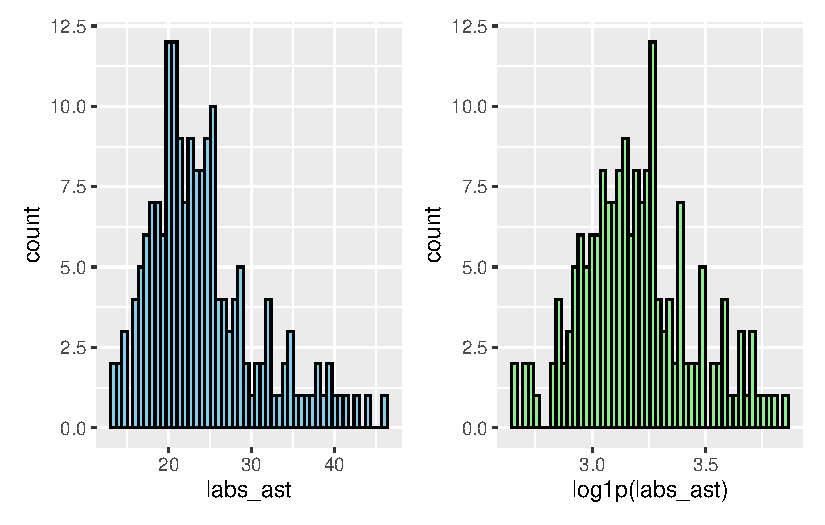
\includegraphics{Outcomes_files/figure-pdf/labs_ast_1-1.pdf}

\begin{Shaded}
\begin{Highlighting}[]
\CommentTok{\# LMM}
\NormalTok{labs\_ast\_model }\OtherTok{\textless{}{-}} \FunctionTok{lmer}\NormalTok{(}\FunctionTok{log1p}\NormalTok{(labs\_ast) }\SpecialCharTok{\textasciitilde{}}\NormalTok{ allocation\_group }\SpecialCharTok{*}\NormalTok{ visit }\SpecialCharTok{+} 
\NormalTok{(}\DecValTok{1} \SpecialCharTok{|}\NormalTok{ record\_id), }\AttributeTok{data =}\NormalTok{ data\_model)}
\FunctionTok{check\_collinearity}\NormalTok{(labs\_ast\_model)}
\end{Highlighting}
\end{Shaded}

\begin{verbatim}
# Check for Multicollinearity

Low Correlation

                   Term  VIF   VIF 95% CI Increased SE Tolerance Tolerance 95% CI
       allocation_group 1.39 [1.21, 1.74]         1.18      0.72     [0.57, 0.83]
                  visit 3.53 [2.81, 4.54]         1.88      0.28     [0.22, 0.36]
 allocation_group:visit 4.18 [3.30, 5.39]         2.04      0.24     [0.19, 0.30]
\end{verbatim}

\begin{Shaded}
\begin{Highlighting}[]
\CommentTok{\# Sensitivity analysis}
\NormalTok{labs\_ast\_model\_check }\OtherTok{\textless{}{-}} \FunctionTok{sensitivity\_check\_lmer}\NormalTok{(}
    \AttributeTok{model =}\NormalTok{ labs\_ast\_model,}
    \AttributeTok{id\_var =} \StringTok{"record\_id"}\NormalTok{,}
    \AttributeTok{top\_n =} \DecValTok{5}\NormalTok{)}

\CommentTok{\# LMM Sensitivity}
\NormalTok{labs\_ast\_model\_sens }\OtherTok{\textless{}{-}} \FunctionTok{update}\NormalTok{(}\AttributeTok{object =}\NormalTok{ labs\_ast\_model,}
                              \AttributeTok{subset =} \SpecialCharTok{!}\NormalTok{(record\_id }\SpecialCharTok{\%in\%} 
\NormalTok{        labs\_ast\_model\_check}\SpecialCharTok{$}\NormalTok{influential\_ids))}
\CommentTok{\# Influential IDS}
\NormalTok{labs\_ast\_model\_check}\SpecialCharTok{$}\NormalTok{influential\_ids}
\end{Highlighting}
\end{Shaded}

\begin{verbatim}
[1] "4"  "14" "33" "61" "16"
\end{verbatim}

\paragraph{Resumo dos modelos}\label{resumo-dos-modelos}

\begin{Shaded}
\begin{Highlighting}[]
\CommentTok{\# Model comparison}
\FunctionTok{summary}\NormalTok{(labs\_ast\_model)}
\end{Highlighting}
\end{Shaded}

\begin{verbatim}
Linear mixed model fit by REML. t-tests use Satterthwaite's method ['lmerModLmerTest']
Formula: log1p(labs_ast) ~ allocation_group * visit + (1 | record_id)
   Data: data_model

REML criterion at convergence: 5.8

Scaled residuals: 
     Min       1Q   Median       3Q      Max 
-2.72864 -0.55023 -0.04259  0.56429  2.70480 

Random effects:
 Groups    Name        Variance Std.Dev.
 record_id (Intercept) 0.03007  0.1734  
 Residual              0.03385  0.1840  
Number of obs: 179, groups:  record_id, 75

Fixed effects:
                                 Estimate Std. Error         df t value Pr(>|t|)    
(Intercept)                      3.211717   0.041563 126.794430  77.273   <2e-16 ***
allocation_groupGrupo B         -0.020671   0.058392 126.794430  -0.354    0.724    
visit2                          -0.008428   0.045718 106.361849  -0.184    0.854    
visit3                          -0.009289   0.049356 109.412475  -0.188    0.851    
allocation_groupGrupo B:visit2  -0.015833   0.066802 109.278386  -0.237    0.813    
allocation_groupGrupo B:visit3   0.025422   0.071565 111.735957   0.355    0.723    
---
Signif. codes:  0 '***' 0.001 '**' 0.01 '*' 0.05 '.' 0.1 ' ' 1

Correlation of Fixed Effects:
            (Intr) all_GB visit2 visit3 a_GB:2
allctn_grGB -0.712                            
visit2      -0.481  0.343                     
visit3      -0.446  0.317  0.442              
allctn_GB:2  0.330 -0.463 -0.684 -0.303       
allctn_GB:3  0.308 -0.432 -0.305 -0.690  0.424
\end{verbatim}

\begin{Shaded}
\begin{Highlighting}[]
\FunctionTok{summary}\NormalTok{(labs\_ast\_model\_sens)}
\end{Highlighting}
\end{Shaded}

\begin{verbatim}
Linear mixed model fit by REML. t-tests use Satterthwaite's method ['lmerModLmerTest']
Formula: log1p(labs_ast) ~ allocation_group * visit + (1 | record_id)
   Data: data_model
 Subset: !(record_id %in% labs_ast_model_check$influential_ids)

REML criterion at convergence: -33.2

Scaled residuals: 
     Min       1Q   Median       3Q      Max 
-1.91122 -0.53274 -0.03816  0.58631  1.89195 

Random effects:
 Groups    Name        Variance Std.Dev.
 record_id (Intercept) 0.03382  0.1839  
 Residual              0.02259  0.1503  
Number of obs: 166, groups:  record_id, 70

Fixed effects:
                                Estimate Std. Error        df t value Pr(>|t|)    
(Intercept)                      3.22105    0.04015 100.92953  80.229   <2e-16 ***
allocation_groupGrupo B         -0.04417    0.05678 100.92953  -0.778    0.438    
visit2                          -0.01756    0.03879  95.56884  -0.453    0.652    
visit3                          -0.03571    0.04157  97.13735  -0.859    0.392    
allocation_groupGrupo B:visit2  -0.02157    0.05710  97.80899  -0.378    0.706    
allocation_groupGrupo B:visit3   0.06882    0.06184  99.31712   1.113    0.268    
---
Signif. codes:  0 '***' 0.001 '**' 0.01 '*' 0.05 '.' 0.1 ' ' 1

Correlation of Fixed Effects:
            (Intr) all_GB visit2 visit3 a_GB:2
allctn_grGB -0.707                            
visit2      -0.414  0.293                     
visit3      -0.387  0.274  0.450              
allctn_GB:2  0.282 -0.398 -0.679 -0.306       
allctn_GB:3  0.260 -0.368 -0.302 -0.672  0.430
\end{verbatim}

\begin{Shaded}
\begin{Highlighting}[]
\NormalTok{labs\_ast\_model\_check}\SpecialCharTok{$}\NormalTok{comparison\_table}
\end{Highlighting}
\end{Shaded}

\begin{verbatim}
# A tibble: 16 x 6
   Model       term                           estimate std.error statistic    p.value
   <chr>       <chr>                             <dbl>     <dbl>     <dbl>      <dbl>
 1 Original    (Intercept)                     3.21       0.0416    77.3    1.64e-108
 2 Sensitivity (Intercept)                     3.22       0.0401    80.2    3.09e- 93
 3 Original    allocation_groupGrupo B        -0.0207     0.0584    -0.354  7.24e-  1
 4 Sensitivity allocation_groupGrupo B        -0.0442     0.0568    -0.778  4.38e-  1
 5 Original    allocation_groupGrupo B:visit2 -0.0158     0.0668    -0.237  8.13e-  1
 6 Sensitivity allocation_groupGrupo B:visit2 -0.0216     0.0571    -0.378  7.06e-  1
 7 Original    allocation_groupGrupo B:visit3  0.0254     0.0716     0.355  7.23e-  1
 8 Sensitivity allocation_groupGrupo B:visit3  0.0688     0.0618     1.11   2.68e-  1
 9 Original    sd__(Intercept)                 0.173     NA         NA     NA        
10 Sensitivity sd__(Intercept)                 0.184     NA         NA     NA        
11 Original    sd__Observation                 0.184     NA         NA     NA        
12 Sensitivity sd__Observation                 0.150     NA         NA     NA        
13 Original    visit2                         -0.00843    0.0457    -0.184  8.54e-  1
14 Sensitivity visit2                         -0.0176     0.0388    -0.453  6.52e-  1
15 Original    visit3                         -0.00929    0.0494    -0.188  8.51e-  1
16 Sensitivity visit3                         -0.0357     0.0416    -0.859  3.92e-  1
\end{verbatim}

\begin{Shaded}
\begin{Highlighting}[]
\NormalTok{labs\_ast\_3performance }\OtherTok{\textless{}{-}}\NormalTok{ performance}\SpecialCharTok{::}\FunctionTok{compare\_performance}\NormalTok{(}
\NormalTok{    labs\_ast\_model, }
\NormalTok{    labs\_ast\_model\_sens)}
\NormalTok{labs\_ast\_3performance}
\end{Highlighting}
\end{Shaded}

\begin{verbatim}
# Comparison of Model Performance Indices

Name                |           Model |  AIC (weights) | AICc (weights) |  BIC (weights) | R2 (cond.) | R2 (marg.) |   ICC |  RMSE | Sigma
------------------------------------------------------------------------------------------------------------------------------------------
labs_ast_model      | lmerModLmerTest | 1139.5 (<.001) | 1140.3 (<.001) | 1165.0 (<.001) |      0.472 |      0.003 | 0.470 | 0.154 | 0.184
labs_ast_model_sens | lmerModLmerTest | 1014.1 (>.999) | 1015.0 (>.999) | 1039.0 (>.999) |      0.605 |      0.013 | 0.600 | 0.122 | 0.150
\end{verbatim}

\begin{Shaded}
\begin{Highlighting}[]
\NormalTok{performance}\SpecialCharTok{::}\FunctionTok{check\_model}\NormalTok{(labs\_ast\_model) }
\end{Highlighting}
\end{Shaded}

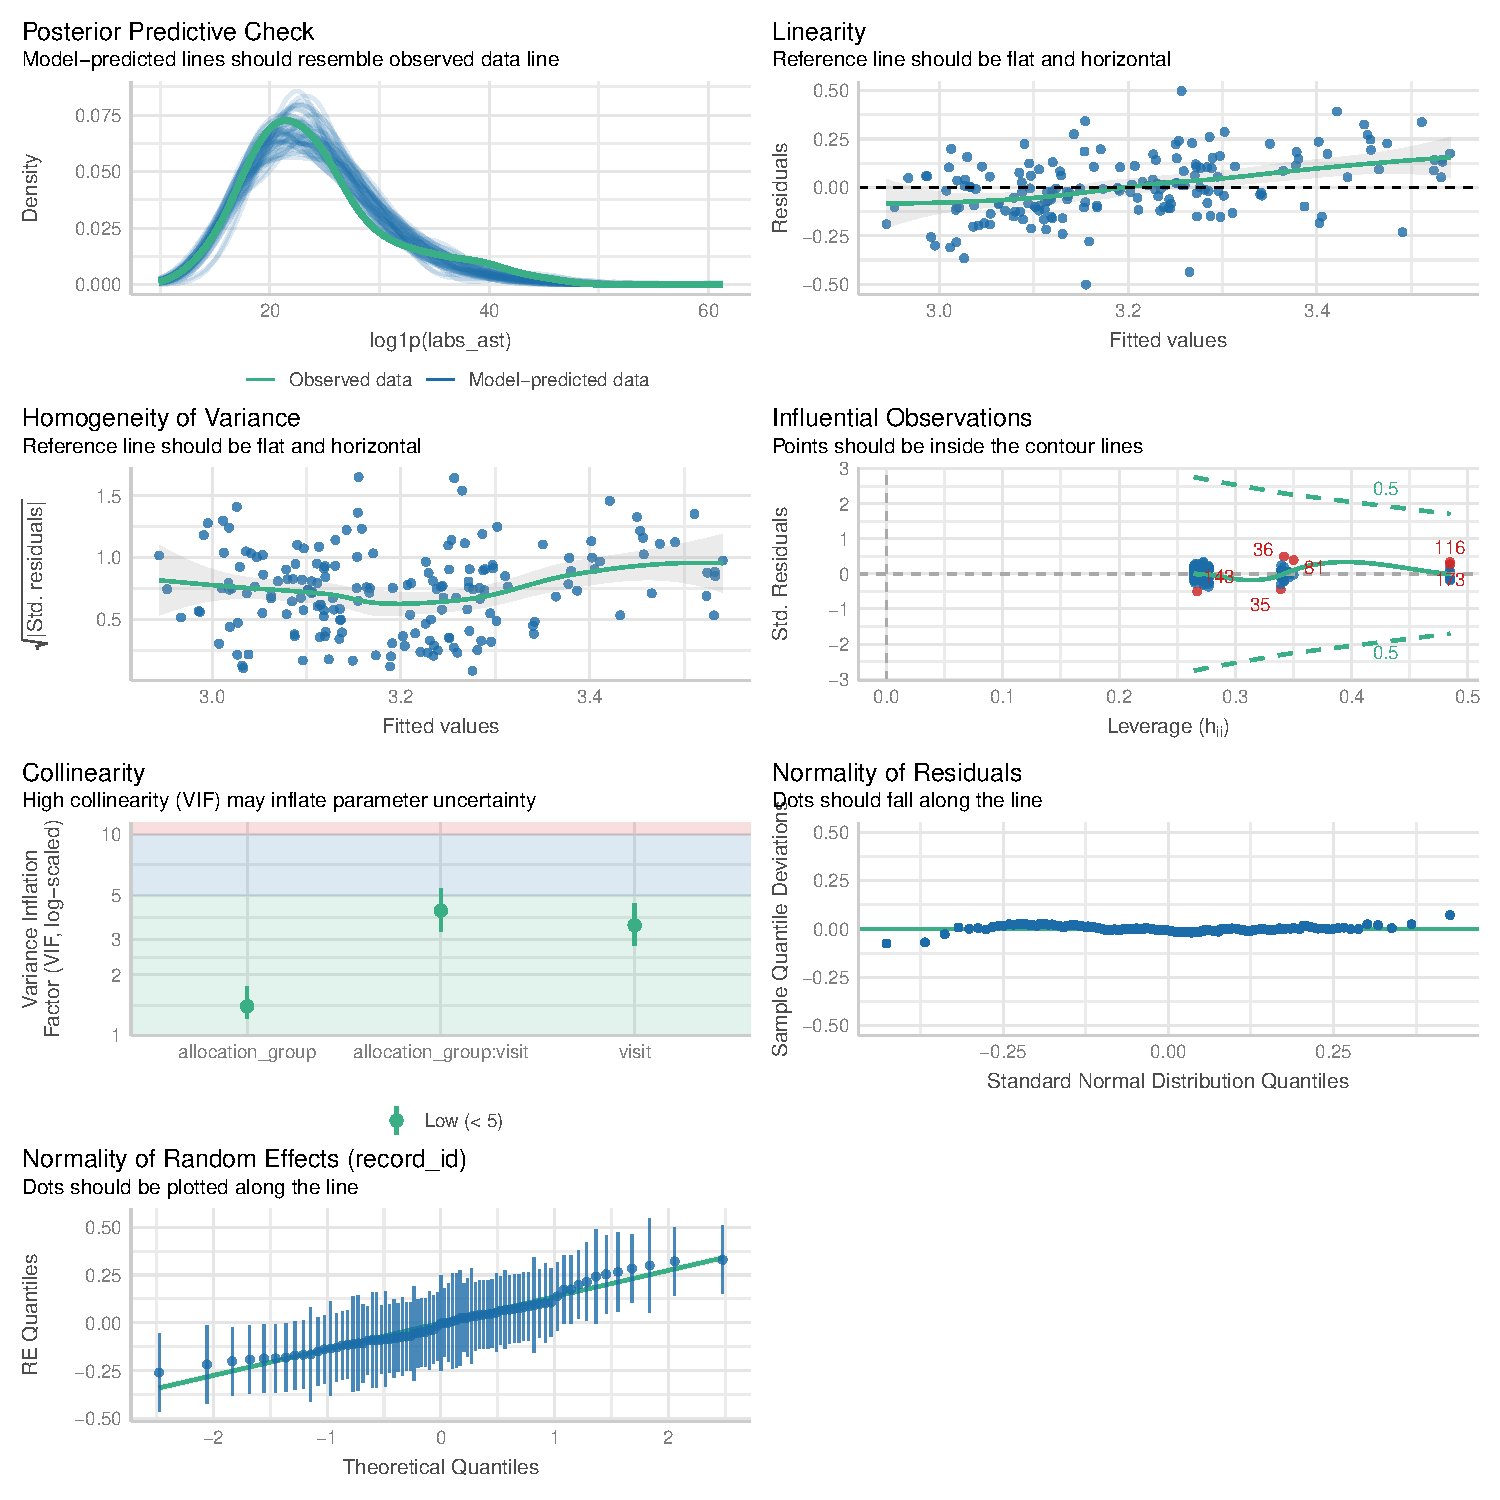
\includegraphics{Outcomes_files/figure-pdf/labs_ast_4-1.pdf}

\begin{Shaded}
\begin{Highlighting}[]
\NormalTok{performance}\SpecialCharTok{::}\FunctionTok{check\_model}\NormalTok{(labs\_ast\_model\_sens)}
\end{Highlighting}
\end{Shaded}

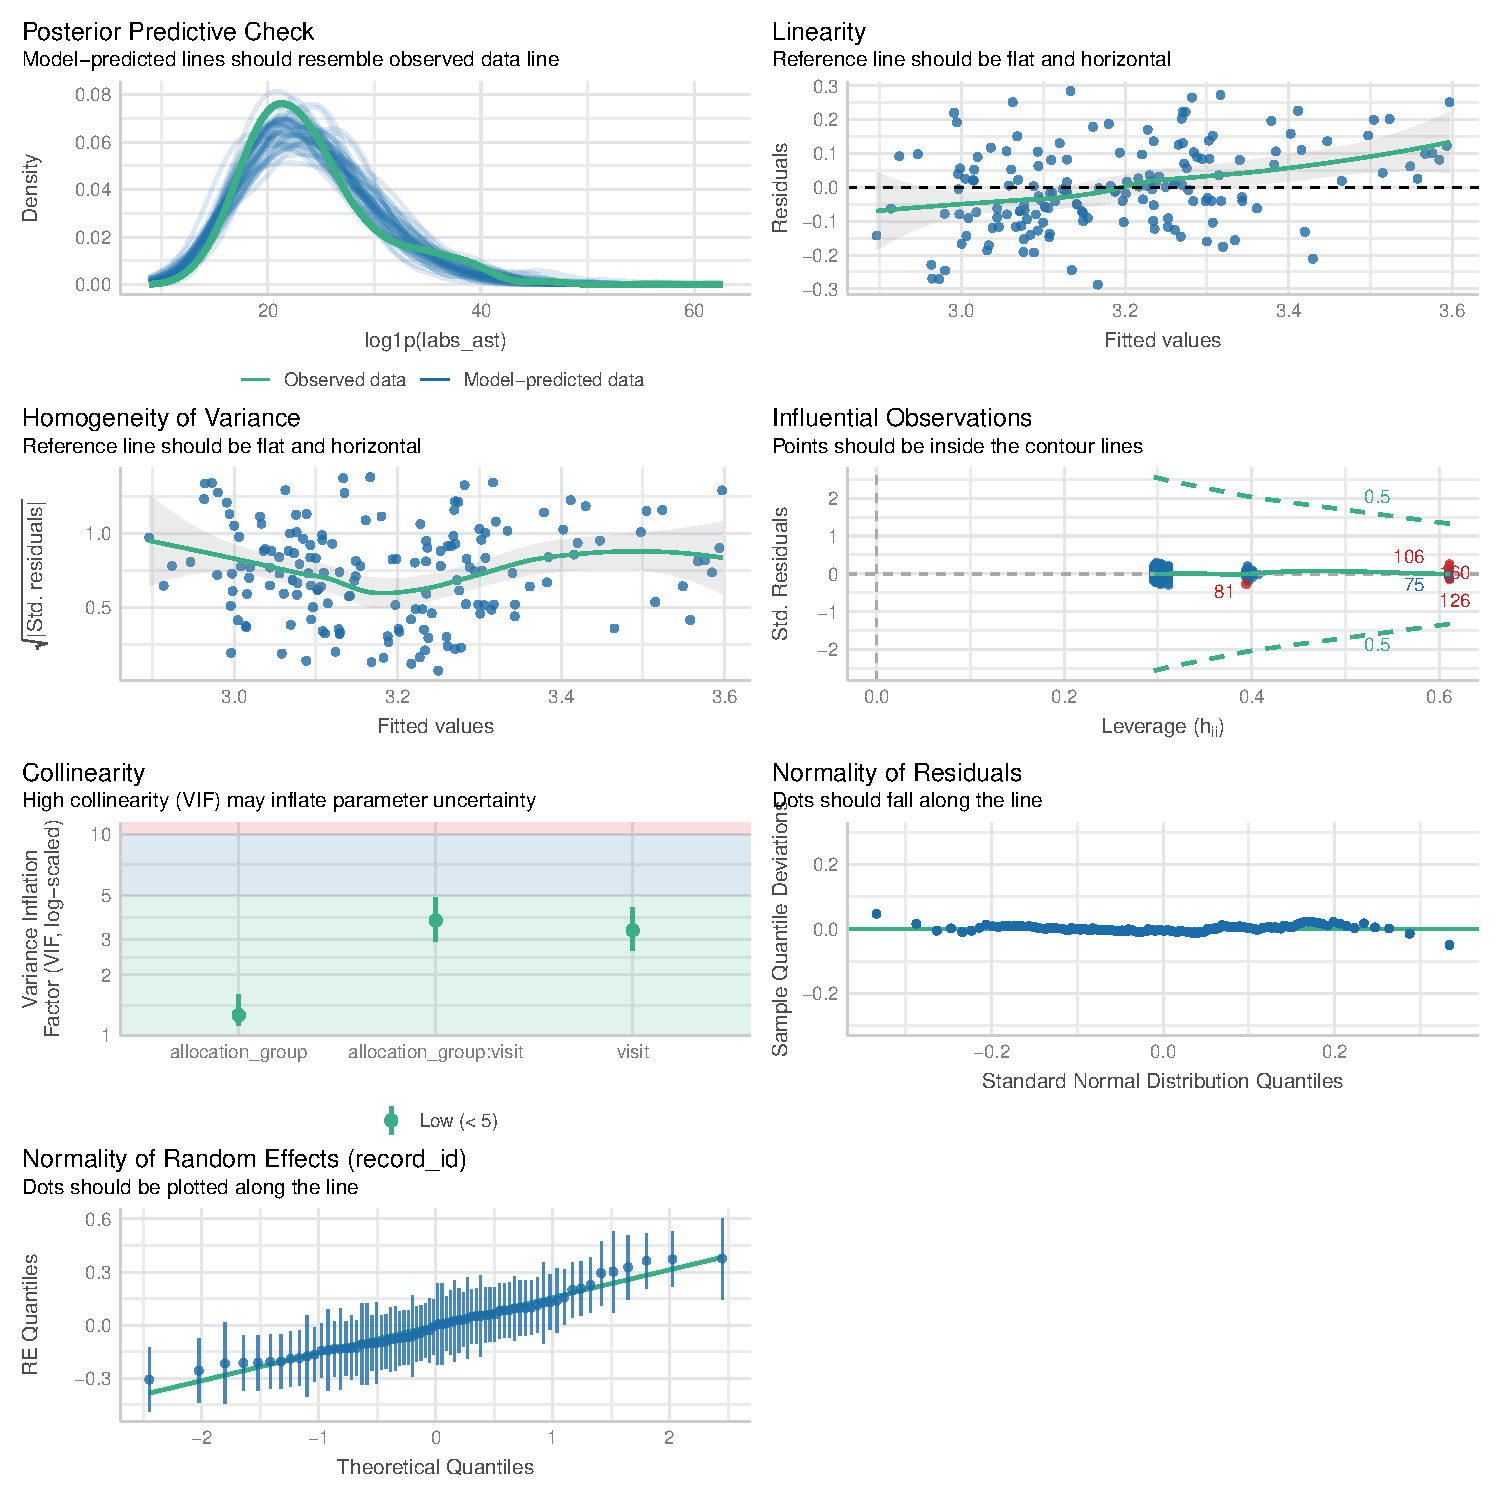
\includegraphics{Outcomes_files/figure-pdf/labs_ast_4-2.pdf}

\paragraph{Médias Marginais
Estimadas}\label{muxe9dias-marginais-estimadas}

\subparagraph{Todos os dados}\label{todos-os-dados}

\begin{Shaded}
\begin{Highlighting}[]
\CommentTok{\# Get EMMs for each group at each visit (All data)}
\NormalTok{labs\_ast\_raw\_emm }\OtherTok{\textless{}{-}}\NormalTok{ emmeans}\SpecialCharTok{::}\FunctionTok{emmeans}\NormalTok{(}
\NormalTok{    labs\_ast\_model, }
    \SpecialCharTok{\textasciitilde{}}\NormalTok{ allocation\_group }\SpecialCharTok{*}\NormalTok{ visit}
\NormalTok{)}

\NormalTok{labs\_ast\_raw\_emm }\OtherTok{\textless{}{-}} \FunctionTok{regrid}\NormalTok{(labs\_ast\_raw\_emm)}

\CommentTok{\# Table of marginal means}
\CommentTok{\# labs\_ast\_raw\_emm}

\CommentTok{\# Pairwise comparisons: Between groups at each visit}
\NormalTok{emmeans}\SpecialCharTok{::}\FunctionTok{contrast}\NormalTok{(labs\_ast\_raw\_emm,}
\AttributeTok{method =} \StringTok{"pairwise"}\NormalTok{, }\AttributeTok{by =} \StringTok{"visit"}\NormalTok{,}
\AttributeTok{adjust =} \StringTok{"bonferroni"}\NormalTok{) }\SpecialCharTok{\%\textgreater{}\%} \FunctionTok{summary}\NormalTok{(}\AttributeTok{infer =} \FunctionTok{c}\NormalTok{(}\ConstantTok{TRUE}\NormalTok{, }\ConstantTok{TRUE}\NormalTok{))}
\end{Highlighting}
\end{Shaded}

\begin{verbatim}
visit = 1:
 contrast          estimate   SE  df lower.CL upper.CL t.ratio p.value
 Grupo A - Grupo B    0.508 1.43 128    -2.33     3.35   0.354  0.7240

visit = 2:
 contrast          estimate   SE  df lower.CL upper.CL t.ratio p.value
 Grupo A - Grupo B    0.882 1.58 142    -2.24     4.00   0.559  0.5771

visit = 3:
 contrast          estimate   SE  df lower.CL upper.CL t.ratio p.value
 Grupo A - Grupo B   -0.117 1.73 157    -3.54     3.31  -0.068  0.9462

Degrees-of-freedom method: inherited from kenward-roger when re-gridding 
Confidence level used: 0.95 
\end{verbatim}

\begin{Shaded}
\begin{Highlighting}[]
\CommentTok{\# Pairwise comparisons: Changes over time within each group}
\NormalTok{emmeans}\SpecialCharTok{::}\FunctionTok{contrast}\NormalTok{(labs\_ast\_raw\_emm,}
\AttributeTok{method =} \StringTok{"pairwise"}\NormalTok{, }\AttributeTok{by =} \StringTok{"allocation\_group"}\NormalTok{,}
\AttributeTok{adjust =} \StringTok{"bonferroni"}\NormalTok{) }\SpecialCharTok{\%\textgreater{}\%} \FunctionTok{summary}\NormalTok{(}\AttributeTok{infer =} \FunctionTok{c}\NormalTok{(}\ConstantTok{TRUE}\NormalTok{, }\ConstantTok{TRUE}\NormalTok{))}
\end{Highlighting}
\end{Shaded}

\begin{verbatim}
allocation_group = Grupo A:
 contrast        estimate   SE  df lower.CL upper.CL t.ratio p.value
 visit1 - visit2   0.2083 1.13 128    -2.53     2.95   0.184  1.0000
 visit1 - visit3   0.2295 1.22 128    -2.73     3.19   0.188  1.0000
 visit2 - visit3   0.0212 1.24 142    -2.98     3.02   0.017  1.0000

allocation_group = Grupo B:
 contrast        estimate   SE  df lower.CL upper.CL t.ratio p.value
 visit1 - visit2   0.5828 1.17 128    -2.25     3.42   0.499  1.0000
 visit1 - visit3  -0.3954 1.28 128    -3.49     2.70  -0.310  1.0000
 visit2 - visit3  -0.9782 1.33 155    -4.20     2.24  -0.735  1.0000

Degrees-of-freedom method: inherited from kenward-roger when re-gridding 
Confidence level used: 0.95 
Conf-level adjustment: bonferroni method for 3 estimates 
P value adjustment: bonferroni method for 3 tests 
\end{verbatim}

\begin{Shaded}
\begin{Highlighting}[]
\CommentTok{\# Plot of marginal means}
\FunctionTok{plot}\NormalTok{(labs\_ast\_raw\_emm, }\AttributeTok{comparisons =} \ConstantTok{TRUE}\NormalTok{)}
\end{Highlighting}
\end{Shaded}

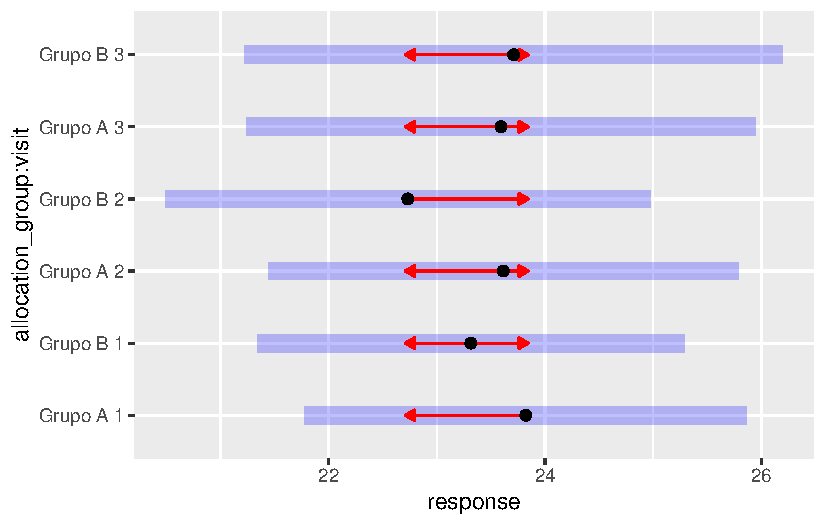
\includegraphics{Outcomes_files/figure-pdf/labs_ast_raw_emm-1.pdf}

\subparagraph{Análise de
sensibilidade}\label{anuxe1lise-de-sensibilidade}

\begin{Shaded}
\begin{Highlighting}[]
\CommentTok{\# Get EMMs for each group at each visit (Sensitivity Analysis)}
\NormalTok{labs\_ast\_emm }\OtherTok{\textless{}{-}}\NormalTok{ emmeans}\SpecialCharTok{::}\FunctionTok{emmeans}\NormalTok{(}
\NormalTok{    labs\_ast\_model\_sens, }
    \SpecialCharTok{\textasciitilde{}}\NormalTok{ allocation\_group }\SpecialCharTok{*}\NormalTok{ visit}
\NormalTok{)}

\NormalTok{labs\_ast\_emm }\OtherTok{\textless{}{-}} \FunctionTok{regrid}\NormalTok{(labs\_ast\_emm)}

\CommentTok{\# Table of marginal means}
\CommentTok{\# labs\_ast\_emm}

\CommentTok{\# Pairwise comparisons: Between groups at each visit}
\NormalTok{emmeans}\SpecialCharTok{::}\FunctionTok{contrast}\NormalTok{(labs\_ast\_emm,}
\AttributeTok{method =} \StringTok{"pairwise"}\NormalTok{, }\AttributeTok{by =} \StringTok{"visit"}\NormalTok{,}
\AttributeTok{adjust =} \StringTok{"bonferroni"}\NormalTok{) }\SpecialCharTok{\%\textgreater{}\%} \FunctionTok{summary}\NormalTok{(}\AttributeTok{infer =} \FunctionTok{c}\NormalTok{(}\ConstantTok{TRUE}\NormalTok{, }\ConstantTok{TRUE}\NormalTok{))}
\end{Highlighting}
\end{Shaded}

\begin{verbatim}
visit = 1:
 contrast          estimate   SE  df lower.CL upper.CL t.ratio p.value
 Grupo A - Grupo B    1.083 1.39 104    -1.68     3.84   0.778  0.4386

visit = 2:
 contrast          estimate   SE  df lower.CL upper.CL t.ratio p.value
 Grupo A - Grupo B    1.566 1.49 118    -1.38     4.51   1.052  0.2948

visit = 3:
 contrast          estimate   SE  df lower.CL upper.CL t.ratio p.value
 Grupo A - Grupo B   -0.603 1.64 132    -3.85     2.64  -0.368  0.7136

Degrees-of-freedom method: inherited from kenward-roger when re-gridding 
Confidence level used: 0.95 
\end{verbatim}

\begin{Shaded}
\begin{Highlighting}[]
\CommentTok{\# Pairwise comparisons: Changes over time within each group}
\NormalTok{emmeans}\SpecialCharTok{::}\FunctionTok{contrast}\NormalTok{(labs\_ast\_emm,}
\AttributeTok{method =} \StringTok{"pairwise"}\NormalTok{, }\AttributeTok{by =} \StringTok{"allocation\_group"}\NormalTok{,}
\AttributeTok{adjust =} \StringTok{"bonferroni"}\NormalTok{) }\SpecialCharTok{\%\textgreater{}\%} \FunctionTok{summary}\NormalTok{(}\AttributeTok{infer =} \FunctionTok{c}\NormalTok{(}\ConstantTok{TRUE}\NormalTok{, }\ConstantTok{TRUE}\NormalTok{))}
\end{Highlighting}
\end{Shaded}

\begin{verbatim}
allocation_group = Grupo A:
 contrast        estimate    SE  df lower.CL upper.CL t.ratio p.value
 visit1 - visit2    0.436 0.963 104    -1.91     2.78   0.453  1.0000
 visit1 - visit3    0.879 1.020 104    -1.60     3.36   0.861  1.0000
 visit2 - visit3    0.443 1.030 118    -2.06     2.94   0.430  1.0000

allocation_group = Grupo B:
 contrast        estimate    SE  df lower.CL upper.CL t.ratio p.value
 visit1 - visit2    0.920 0.983 104    -1.47     3.31   0.936  1.0000
 visit1 - visit3   -0.807 1.130 104    -3.55     1.93  -0.716  1.0000
 visit2 - visit3   -1.727 1.150 131    -4.51     1.06  -1.505  0.4043

Degrees-of-freedom method: inherited from kenward-roger when re-gridding 
Confidence level used: 0.95 
Conf-level adjustment: bonferroni method for 3 estimates 
P value adjustment: bonferroni method for 3 tests 
\end{verbatim}

\begin{Shaded}
\begin{Highlighting}[]
\CommentTok{\# Plot of marginal means}
\FunctionTok{plot}\NormalTok{(labs\_ast\_emm, }\AttributeTok{comparisons =} \ConstantTok{TRUE}\NormalTok{)}
\end{Highlighting}
\end{Shaded}

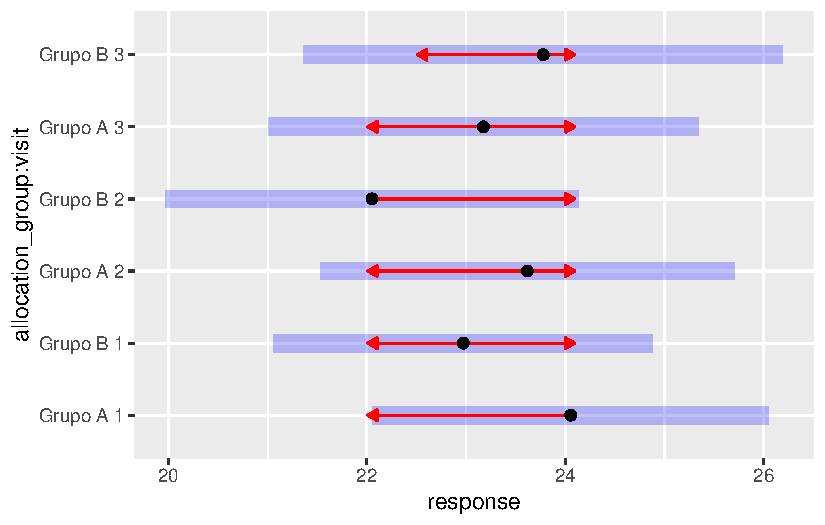
\includegraphics{Outcomes_files/figure-pdf/labs_ast_sens_emm-1.pdf}

\paragraph{Resultado}\label{resultado}

No modelo ajustado para os níveis de AST, não foram observadas
diferenças estatisticamente significativas entre os grupos em nenhum dos
três momentos avaliados. Da mesma forma, não houve mudanças
significativas ao longo do tempo dentro de cada grupo. A análise de
sensibilidade não alterou substancialmente os resultados. As estimativas
permaneceram estáveis e as diferenças entre os grupos e ao longo do
tempo continuaram não significativas. As estimativas, intervalos de
confiança de 95\% e valores de p estão apresentados na
Tabela~\ref{tbl-ast}.

\begin{longtable}[]{@{}
  >{\raggedright\arraybackslash}p{(\columnwidth - 8\tabcolsep) * \real{0.2000}}
  >{\raggedright\arraybackslash}p{(\columnwidth - 8\tabcolsep) * \real{0.2000}}
  >{\raggedright\arraybackslash}p{(\columnwidth - 8\tabcolsep) * \real{0.2000}}
  >{\raggedright\arraybackslash}p{(\columnwidth - 8\tabcolsep) * \real{0.2000}}
  >{\raggedright\arraybackslash}p{(\columnwidth - 8\tabcolsep) * \real{0.2000}}@{}}
\caption{Diferenças estimadas dos níveis de Aspartato Aminotransferase
(AST) entre os grupos de alocação (placebo vs Eclipta) e entre visitas
dentro de cada grupo}\label{tbl-ast}\tabularnewline
\toprule\noalign{}
\begin{minipage}[b]{\linewidth}\raggedright
Grupo de comparação
\end{minipage} & \begin{minipage}[b]{\linewidth}\raggedright
Comparação
\end{minipage} & \begin{minipage}[b]{\linewidth}\raggedright
Estimativa
\end{minipage} & \begin{minipage}[b]{\linewidth}\raggedright
IC 95\%
\end{minipage} & \begin{minipage}[b]{\linewidth}\raggedright
p-valor
\end{minipage} \\
\midrule\noalign{}
\endfirsthead
\toprule\noalign{}
\begin{minipage}[b]{\linewidth}\raggedright
Grupo de comparação
\end{minipage} & \begin{minipage}[b]{\linewidth}\raggedright
Comparação
\end{minipage} & \begin{minipage}[b]{\linewidth}\raggedright
Estimativa
\end{minipage} & \begin{minipage}[b]{\linewidth}\raggedright
IC 95\%
\end{minipage} & \begin{minipage}[b]{\linewidth}\raggedright
p-valor
\end{minipage} \\
\midrule\noalign{}
\endhead
\bottomrule\noalign{}
\endlastfoot
Entre grupos & Visita 1 & 0,51 & {[}-2,33 ; 3,35{]} & 0,724 \\
Entre grupos & Visita 2 & 0,88 & {[}-2,24 ; 4,00{]} & 0,577 \\
Entre grupos & Visita 3 & -0,12 & {[}-3,54 ; 3,31{]} & 0,946 \\
Grupo Placebo & Visita 1 - Visita 2 & 0,21 & {[}-2,53 ; 2,95{]} &
1,000 \\
Grupo Placebo & Visita 1 - Visita 3 & 0,23 & {[}-2,73 ; 3,19{]} &
1,000 \\
Grupo Placebo & Visita 2 - Visita 3 & 0,02 & {[}-2,98 ; 3,02{]} &
1,000 \\
Grupo Eclipta & Visita 1 - Visita 2 & 0,58 & {[}-2,25 ; 3,42{]} &
1,000 \\
Grupo Eclipta & Visita 1 - Visita 3 & -0,40 & {[}-3,49 ; 2,70{]} &
1,000 \\
Grupo Eclipta & Visita 2 - Visita 3 & -0,98 & {[}-4,20 ; 2,24{]} &
1,000 \\
\end{longtable}

\begin{Shaded}
\begin{Highlighting}[]
\FunctionTok{ggplot}\NormalTok{(}
    \AttributeTok{data =}\NormalTok{ data\_model, }
    \FunctionTok{aes}\NormalTok{(}
        \AttributeTok{x =} \FunctionTok{as.factor}\NormalTok{(visit),}
        \AttributeTok{y =}\NormalTok{ labs\_ast,}
        \AttributeTok{group =}\NormalTok{ record\_id,}
\NormalTok{    )}
\NormalTok{) }\SpecialCharTok{+}
    \FunctionTok{geom\_line}\NormalTok{(}\AttributeTok{alpha =} \FloatTok{0.5}\NormalTok{) }\SpecialCharTok{+}
    \FunctionTok{geom\_point}\NormalTok{(}\AttributeTok{alpha =} \FloatTok{0.7}\NormalTok{) }\SpecialCharTok{+}
    \FunctionTok{geom\_smooth}\NormalTok{(}
        \FunctionTok{aes}\NormalTok{(}\AttributeTok{group =}\NormalTok{ allocation\_group),}
        \AttributeTok{method =} \StringTok{"lm"}\NormalTok{,}
        \AttributeTok{se =} \ConstantTok{TRUE}\NormalTok{,}
        \AttributeTok{linewidth =} \DecValTok{1}
\NormalTok{    ) }\SpecialCharTok{+}
    \FunctionTok{labs}\NormalTok{(}\AttributeTok{title =} \StringTok{"All data"}\NormalTok{) }\SpecialCharTok{+}
    \FunctionTok{facet\_wrap}\NormalTok{(}\SpecialCharTok{\textasciitilde{}}\NormalTok{ allocation\_group)}
\end{Highlighting}
\end{Shaded}

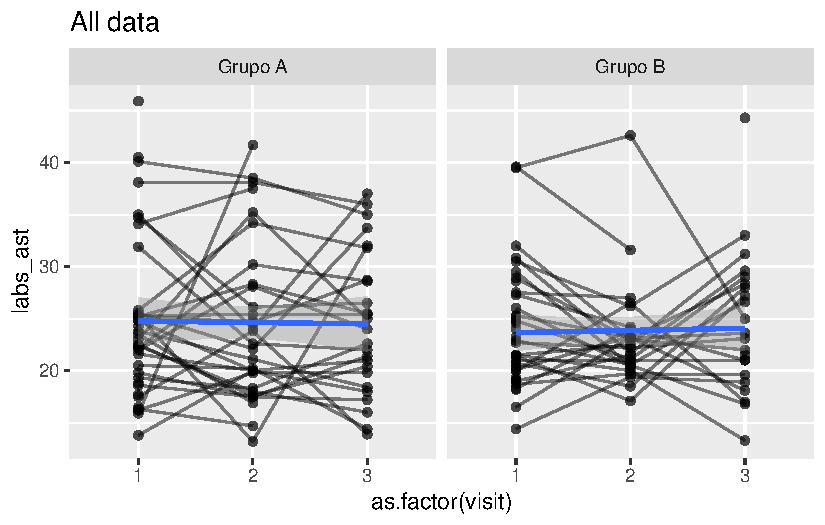
\includegraphics{Outcomes_files/figure-pdf/labs_ast_6-1.pdf}

\begin{Shaded}
\begin{Highlighting}[]
\NormalTok{data\_model }\SpecialCharTok{\%\textgreater{}\%} 
    \FunctionTok{filter}\NormalTok{(}
        \SpecialCharTok{!}\NormalTok{(record\_id }\SpecialCharTok{\%in\%} 
\NormalTok{        labs\_ast\_model\_check}\SpecialCharTok{$}\NormalTok{influential\_ids)}
\NormalTok{    ) }\SpecialCharTok{\%\textgreater{}\%} 
    \FunctionTok{ggplot}\NormalTok{(}
        \FunctionTok{aes}\NormalTok{(}
            \AttributeTok{x =} \FunctionTok{as.factor}\NormalTok{(visit),}
            \AttributeTok{y =}\NormalTok{ labs\_ast,}
            \AttributeTok{group =}\NormalTok{ record\_id,}
\NormalTok{        )}
\NormalTok{    ) }\SpecialCharTok{+}
    \FunctionTok{geom\_line}\NormalTok{(}\AttributeTok{alpha =} \FloatTok{0.5}\NormalTok{) }\SpecialCharTok{+}
    \FunctionTok{geom\_point}\NormalTok{(}\AttributeTok{alpha =} \FloatTok{0.7}\NormalTok{) }\SpecialCharTok{+}
    \FunctionTok{geom\_smooth}\NormalTok{(}
        \FunctionTok{aes}\NormalTok{(}\AttributeTok{group =}\NormalTok{ allocation\_group),}
        \AttributeTok{method =} \StringTok{"lm"}\NormalTok{,}
        \AttributeTok{se =} \ConstantTok{TRUE}\NormalTok{,}
        \AttributeTok{linewidth =} \DecValTok{1}
\NormalTok{    ) }\SpecialCharTok{+}
    \FunctionTok{labs}\NormalTok{(}\AttributeTok{title =} \StringTok{"Sensitivity analysis"}\NormalTok{) }\SpecialCharTok{+}
    \FunctionTok{facet\_wrap}\NormalTok{(}\SpecialCharTok{\textasciitilde{}}\NormalTok{ allocation\_group)}
\end{Highlighting}
\end{Shaded}

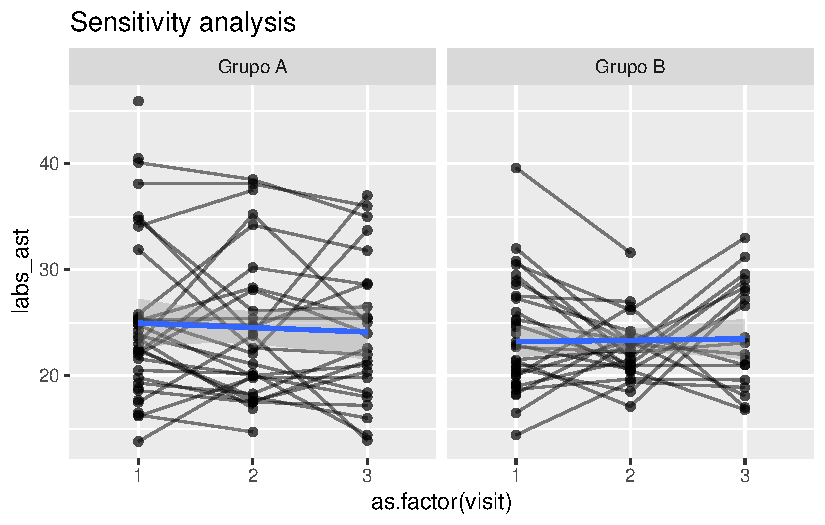
\includegraphics{Outcomes_files/figure-pdf/labs_ast_6-2.pdf}

\subsubsection{Alanina Aminotransferase}\label{alanina-aminotransferase}

\begin{Shaded}
\begin{Highlighting}[]
\CommentTok{\# Plot 1: Raw data}
\NormalTok{labs\_alt\_hist\_1 }\OtherTok{\textless{}{-}}\NormalTok{ data\_model }\SpecialCharTok{\%\textgreater{}\%} 
    \CommentTok{\#filter(}
    \CommentTok{\#    labs\_alt \textless{} 300}
    \CommentTok{\#) \%\textgreater{}\% }
    \FunctionTok{ggplot}\NormalTok{(}\FunctionTok{aes}\NormalTok{(}\AttributeTok{x =}\NormalTok{ labs\_alt)) }\SpecialCharTok{+} 
    \FunctionTok{geom\_histogram}\NormalTok{(}\AttributeTok{bins =} \DecValTok{50}\NormalTok{, }\AttributeTok{fill =} \StringTok{"skyblue"}\NormalTok{, }\AttributeTok{color =} \StringTok{"black"}\NormalTok{)}

\CommentTok{\# Plot 2: Log{-}transformed data}
\NormalTok{labs\_alt\_hist\_2 }\OtherTok{\textless{}{-}}\NormalTok{ data\_model }\SpecialCharTok{\%\textgreater{}\%} 
    \CommentTok{\#filter(}
    \CommentTok{\#    labs\_alt \textless{} 300}
    \CommentTok{\#) \%\textgreater{}\%}
    \FunctionTok{ggplot}\NormalTok{(}\FunctionTok{aes}\NormalTok{(}\AttributeTok{x =} \FunctionTok{log1p}\NormalTok{(labs\_alt))) }\SpecialCharTok{+} 
    \FunctionTok{geom\_histogram}\NormalTok{(}\AttributeTok{bins =} \DecValTok{50}\NormalTok{, }\AttributeTok{fill =} \StringTok{"lightgreen"}\NormalTok{, }\AttributeTok{color =} \StringTok{"black"}\NormalTok{)}

\CommentTok{\# Combine side by side}
\NormalTok{labs\_alt\_hist\_1 }\SpecialCharTok{+}\NormalTok{ labs\_alt\_hist\_2 }\CommentTok{\# library(patchwork)}
\end{Highlighting}
\end{Shaded}

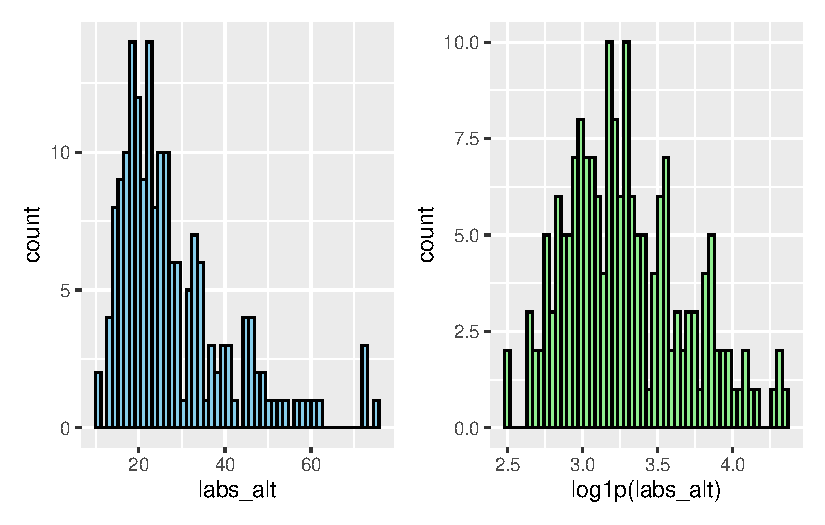
\includegraphics{Outcomes_files/figure-pdf/labs_alt_1-1.pdf}

\begin{Shaded}
\begin{Highlighting}[]
\CommentTok{\# LMM}
\NormalTok{labs\_alt\_model }\OtherTok{\textless{}{-}} \FunctionTok{lmer}\NormalTok{(}\FunctionTok{log1p}\NormalTok{(labs\_alt) }\SpecialCharTok{\textasciitilde{}}\NormalTok{ allocation\_group }\SpecialCharTok{*}\NormalTok{ visit }\SpecialCharTok{+} 
\NormalTok{(}\DecValTok{1} \SpecialCharTok{|}\NormalTok{ record\_id), }\AttributeTok{data =}\NormalTok{ data\_model)}
\FunctionTok{check\_collinearity}\NormalTok{(labs\_alt\_model)}
\end{Highlighting}
\end{Shaded}

\begin{verbatim}
# Check for Multicollinearity

Low Correlation

                   Term  VIF   VIF 95% CI Increased SE Tolerance Tolerance 95% CI
       allocation_group 1.21 [1.08, 1.54]         1.10      0.83     [0.65, 0.92]
                  visit 3.50 [2.79, 4.49]         1.87      0.29     [0.22, 0.36]
 allocation_group:visit 3.84 [3.04, 4.94]         1.96      0.26     [0.20, 0.33]
\end{verbatim}

\begin{Shaded}
\begin{Highlighting}[]
\CommentTok{\# Sensitivity analysis}
\NormalTok{labs\_alt\_model\_check }\OtherTok{\textless{}{-}} \FunctionTok{sensitivity\_check\_lmer}\NormalTok{(}
    \AttributeTok{model =}\NormalTok{ labs\_alt\_model,}
    \AttributeTok{id\_var =} \StringTok{"record\_id"}\NormalTok{,}
    \AttributeTok{top\_n =} \DecValTok{5}\NormalTok{)}

\CommentTok{\# LMM Sensitivity}
\NormalTok{labs\_alt\_model\_sens }\OtherTok{\textless{}{-}} \FunctionTok{update}\NormalTok{(}\AttributeTok{object =}\NormalTok{ labs\_alt\_model,}
                              \AttributeTok{subset =} \SpecialCharTok{!}\NormalTok{(record\_id }\SpecialCharTok{\%in\%} 
\NormalTok{        labs\_alt\_model\_check}\SpecialCharTok{$}\NormalTok{influential\_ids))}
\CommentTok{\# Influential IDS}
\NormalTok{labs\_alt\_model\_check}\SpecialCharTok{$}\NormalTok{influential\_ids}
\end{Highlighting}
\end{Shaded}

\begin{verbatim}
[1] "33" "75" "5"  "58" "63"
\end{verbatim}

\paragraph{Resumo dos modelos}\label{resumo-dos-modelos-1}

\begin{Shaded}
\begin{Highlighting}[]
\CommentTok{\# Model comparison}
\FunctionTok{summary}\NormalTok{(labs\_alt\_model)}
\end{Highlighting}
\end{Shaded}

\begin{verbatim}
Linear mixed model fit by REML. t-tests use Satterthwaite's method ['lmerModLmerTest']
Formula: log1p(labs_alt) ~ allocation_group * visit + (1 | record_id)
   Data: data_model

REML criterion at convergence: 132.2

Scaled residuals: 
     Min       1Q   Median       3Q      Max 
-2.28166 -0.55027 -0.05275  0.54015  2.15582 

Random effects:
 Groups    Name        Variance Std.Dev.
 record_id (Intercept) 0.10863  0.3296  
 Residual              0.05485  0.2342  
Number of obs: 179, groups:  record_id, 75

Fixed effects:
                                Estimate Std. Error        df t value Pr(>|t|)    
(Intercept)                      3.34045    0.06647 102.44387  50.254   <2e-16 ***
allocation_groupGrupo B         -0.10187    0.09338 102.44387  -1.091    0.278    
visit2                          -0.07956    0.05867 103.85033  -1.356    0.178    
visit3                          -0.03364    0.06353 105.34376  -0.529    0.598    
allocation_groupGrupo B:visit2   0.06143    0.08602 105.75034   0.714    0.477    
allocation_groupGrupo B:visit3   0.07920    0.09237 106.88087   0.857    0.393    
---
Signif. codes:  0 '***' 0.001 '**' 0.01 '*' 0.05 '.' 0.1 ' ' 1

Correlation of Fixed Effects:
            (Intr) all_GB visit2 visit3 a_GB:2
allctn_grGB -0.712                            
visit2      -0.380  0.271                     
visit3      -0.351  0.250  0.449              
allctn_GB:2  0.259 -0.364 -0.682 -0.306       
allctn_GB:3  0.241 -0.339 -0.309 -0.688  0.432
\end{verbatim}

\begin{Shaded}
\begin{Highlighting}[]
\FunctionTok{summary}\NormalTok{(labs\_alt\_model\_sens)}
\end{Highlighting}
\end{Shaded}

\begin{verbatim}
Linear mixed model fit by REML. t-tests use Satterthwaite's method ['lmerModLmerTest']
Formula: log1p(labs_alt) ~ allocation_group * visit + (1 | record_id)
   Data: data_model
 Subset: !(record_id %in% labs_alt_model_check$influential_ids)

REML criterion at convergence: 88.4

Scaled residuals: 
     Min       1Q   Median       3Q      Max 
-1.98911 -0.51655 -0.03328  0.57521  2.21076 

Random effects:
 Groups    Name        Variance Std.Dev.
 record_id (Intercept) 0.09385  0.3063  
 Residual              0.04238  0.2059  
Number of obs: 165, groups:  record_id, 70

Fixed effects:
                                Estimate Std. Error        df t value Pr(>|t|)    
(Intercept)                     3.249918   0.064250 90.966334  50.582   <2e-16 ***
allocation_groupGrupo B        -0.013075   0.088373 90.966334  -0.148    0.883    
visit2                         -0.021536   0.055231 93.405160  -0.390    0.697    
visit3                         -0.035422   0.060679 94.750397  -0.584    0.561    
allocation_groupGrupo B:visit2 -0.009275   0.078377 94.689442  -0.118    0.906    
allocation_groupGrupo B:visit3  0.043535   0.085567 95.767451   0.509    0.612    
---
Signif. codes:  0 '***' 0.001 '**' 0.01 '*' 0.05 '.' 0.1 ' ' 1

Correlation of Fixed Effects:
            (Intr) all_GB visit2 visit3 a_GB:2
allctn_grGB -0.727                            
visit2      -0.362  0.263                     
visit3      -0.329  0.239  0.442              
allctn_GB:2  0.255 -0.351 -0.705 -0.311       
allctn_GB:3  0.234 -0.321 -0.313 -0.709  0.434
\end{verbatim}

\begin{Shaded}
\begin{Highlighting}[]
\NormalTok{labs\_alt\_model\_check}\SpecialCharTok{$}\NormalTok{comparison\_table}
\end{Highlighting}
\end{Shaded}

\begin{verbatim}
# A tibble: 16 x 6
   Model       term                           estimate std.error statistic   p.value
   <chr>       <chr>                             <dbl>     <dbl>     <dbl>     <dbl>
 1 Original    (Intercept)                     3.34       0.0665    50.3    5.32e-74
 2 Sensitivity (Intercept)                     3.25       0.0642    50.6    2.13e-68
 3 Original    allocation_groupGrupo B        -0.102      0.0934    -1.09   2.78e- 1
 4 Sensitivity allocation_groupGrupo B        -0.0131     0.0884    -0.148  8.83e- 1
 5 Original    allocation_groupGrupo B:visit2  0.0614     0.0860     0.714  4.77e- 1
 6 Sensitivity allocation_groupGrupo B:visit2 -0.00928    0.0784    -0.118  9.06e- 1
 7 Original    allocation_groupGrupo B:visit3  0.0792     0.0924     0.857  3.93e- 1
 8 Sensitivity allocation_groupGrupo B:visit3  0.0435     0.0856     0.509  6.12e- 1
 9 Original    sd__(Intercept)                 0.330     NA         NA     NA       
10 Sensitivity sd__(Intercept)                 0.306     NA         NA     NA       
11 Original    sd__Observation                 0.234     NA         NA     NA       
12 Sensitivity sd__Observation                 0.206     NA         NA     NA       
13 Original    visit2                         -0.0796     0.0587    -1.36   1.78e- 1
14 Sensitivity visit2                         -0.0215     0.0552    -0.390  6.97e- 1
15 Original    visit3                         -0.0336     0.0635    -0.529  5.98e- 1
16 Sensitivity visit3                         -0.0354     0.0607    -0.584  5.61e- 1
\end{verbatim}

\begin{Shaded}
\begin{Highlighting}[]
\NormalTok{performance}\SpecialCharTok{::}\FunctionTok{compare\_performance}\NormalTok{(}
\NormalTok{    labs\_alt\_model, }
\NormalTok{    labs\_alt\_model\_sens)}
\end{Highlighting}
\end{Shaded}

\begin{verbatim}
# Comparison of Model Performance Indices

Name                |           Model |  AIC (weights) | AICc (weights) |  BIC (weights) | R2 (cond.) | R2 (marg.) |   ICC |  RMSE | Sigma
------------------------------------------------------------------------------------------------------------------------------------------
labs_alt_model      | lmerModLmerTest | 1302.9 (<.001) | 1303.8 (<.001) | 1328.4 (<.001) |      0.668 |      0.011 | 0.664 | 0.187 | 0.234
labs_alt_model_sens | lmerModLmerTest | 1150.5 (>.999) | 1151.4 (>.999) | 1175.3 (>.999) |      0.689 |      0.002 | 0.689 | 0.163 | 0.206
\end{verbatim}

\begin{Shaded}
\begin{Highlighting}[]
\NormalTok{performance}\SpecialCharTok{::}\FunctionTok{check\_model}\NormalTok{(labs\_alt\_model)}
\end{Highlighting}
\end{Shaded}

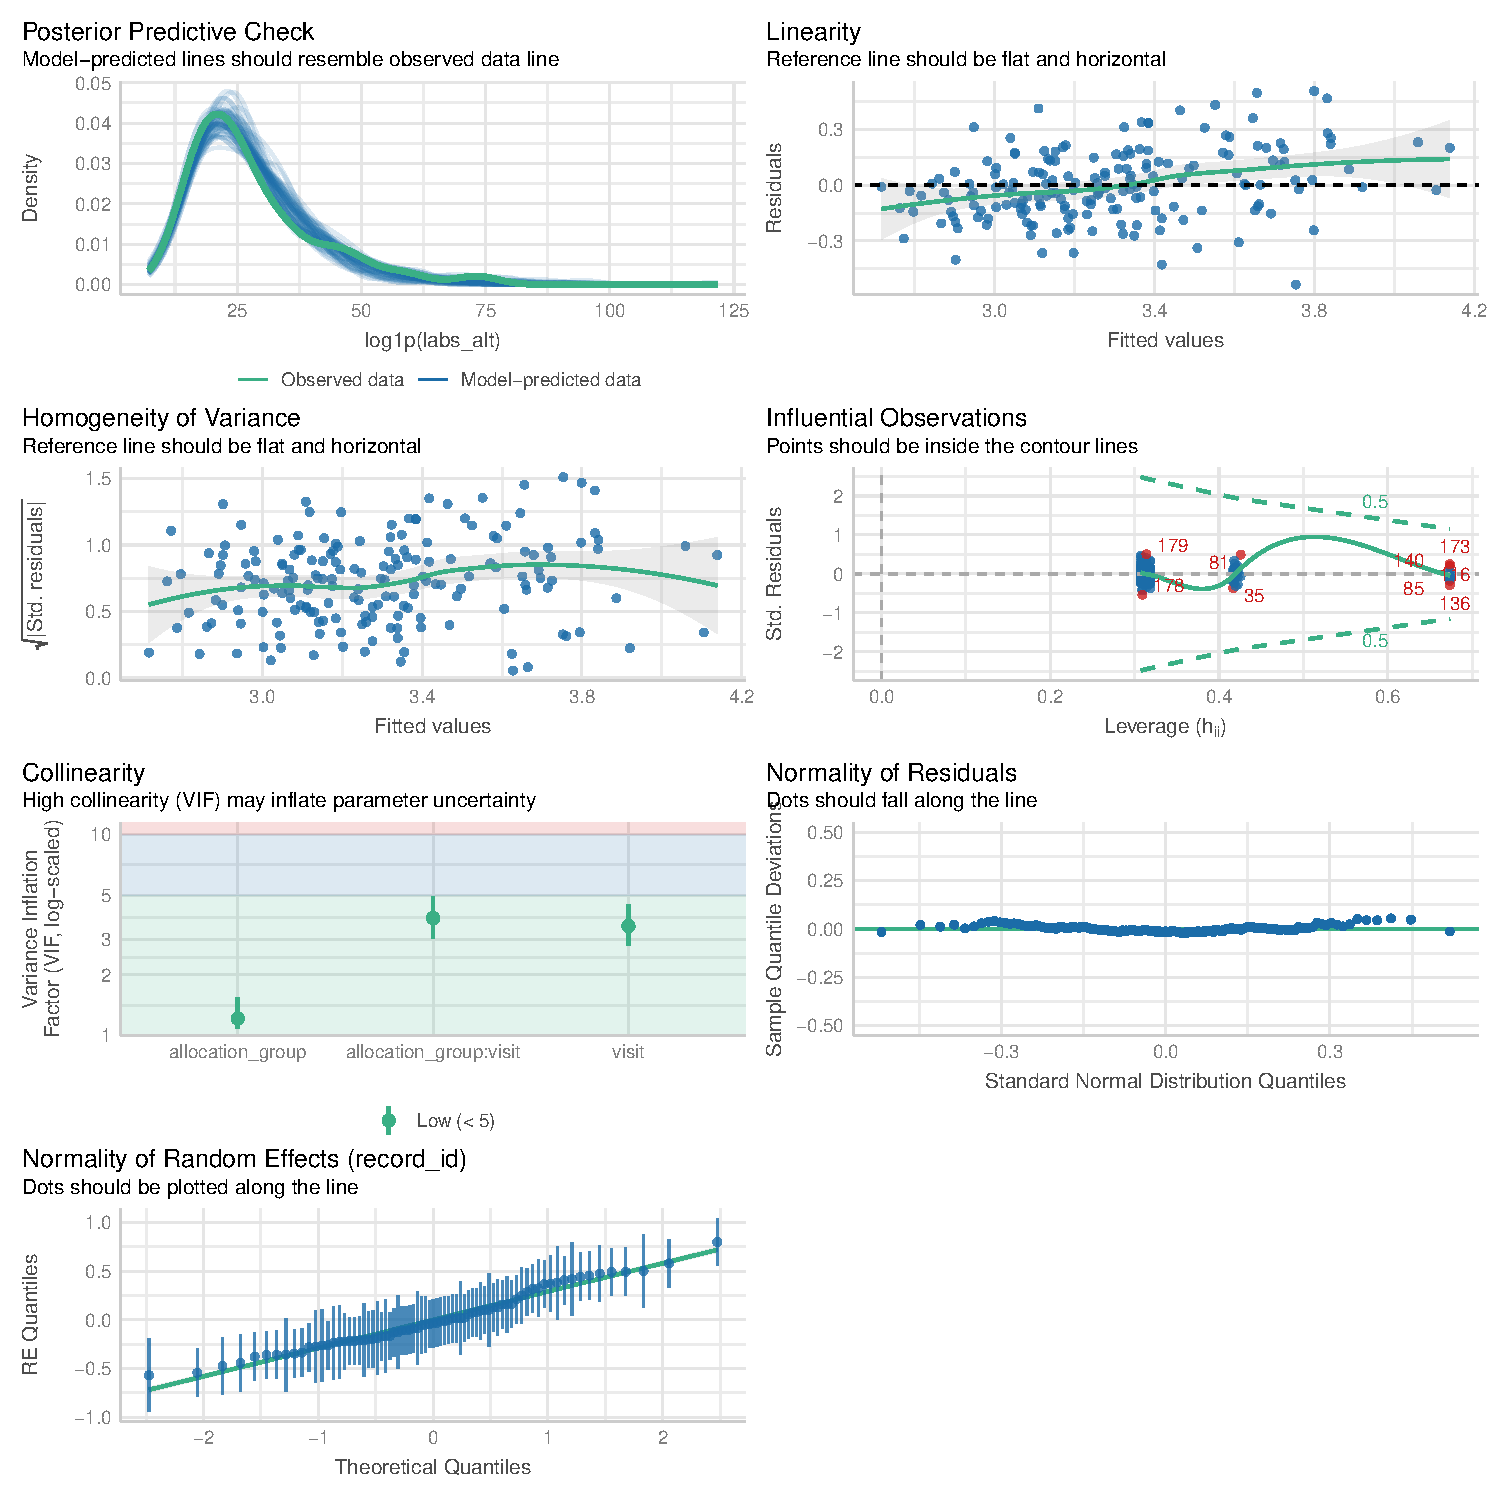
\includegraphics{Outcomes_files/figure-pdf/labs_alt_4-1.pdf}

\begin{Shaded}
\begin{Highlighting}[]
\NormalTok{performance}\SpecialCharTok{::}\FunctionTok{check\_model}\NormalTok{(labs\_alt\_model\_sens)}
\end{Highlighting}
\end{Shaded}

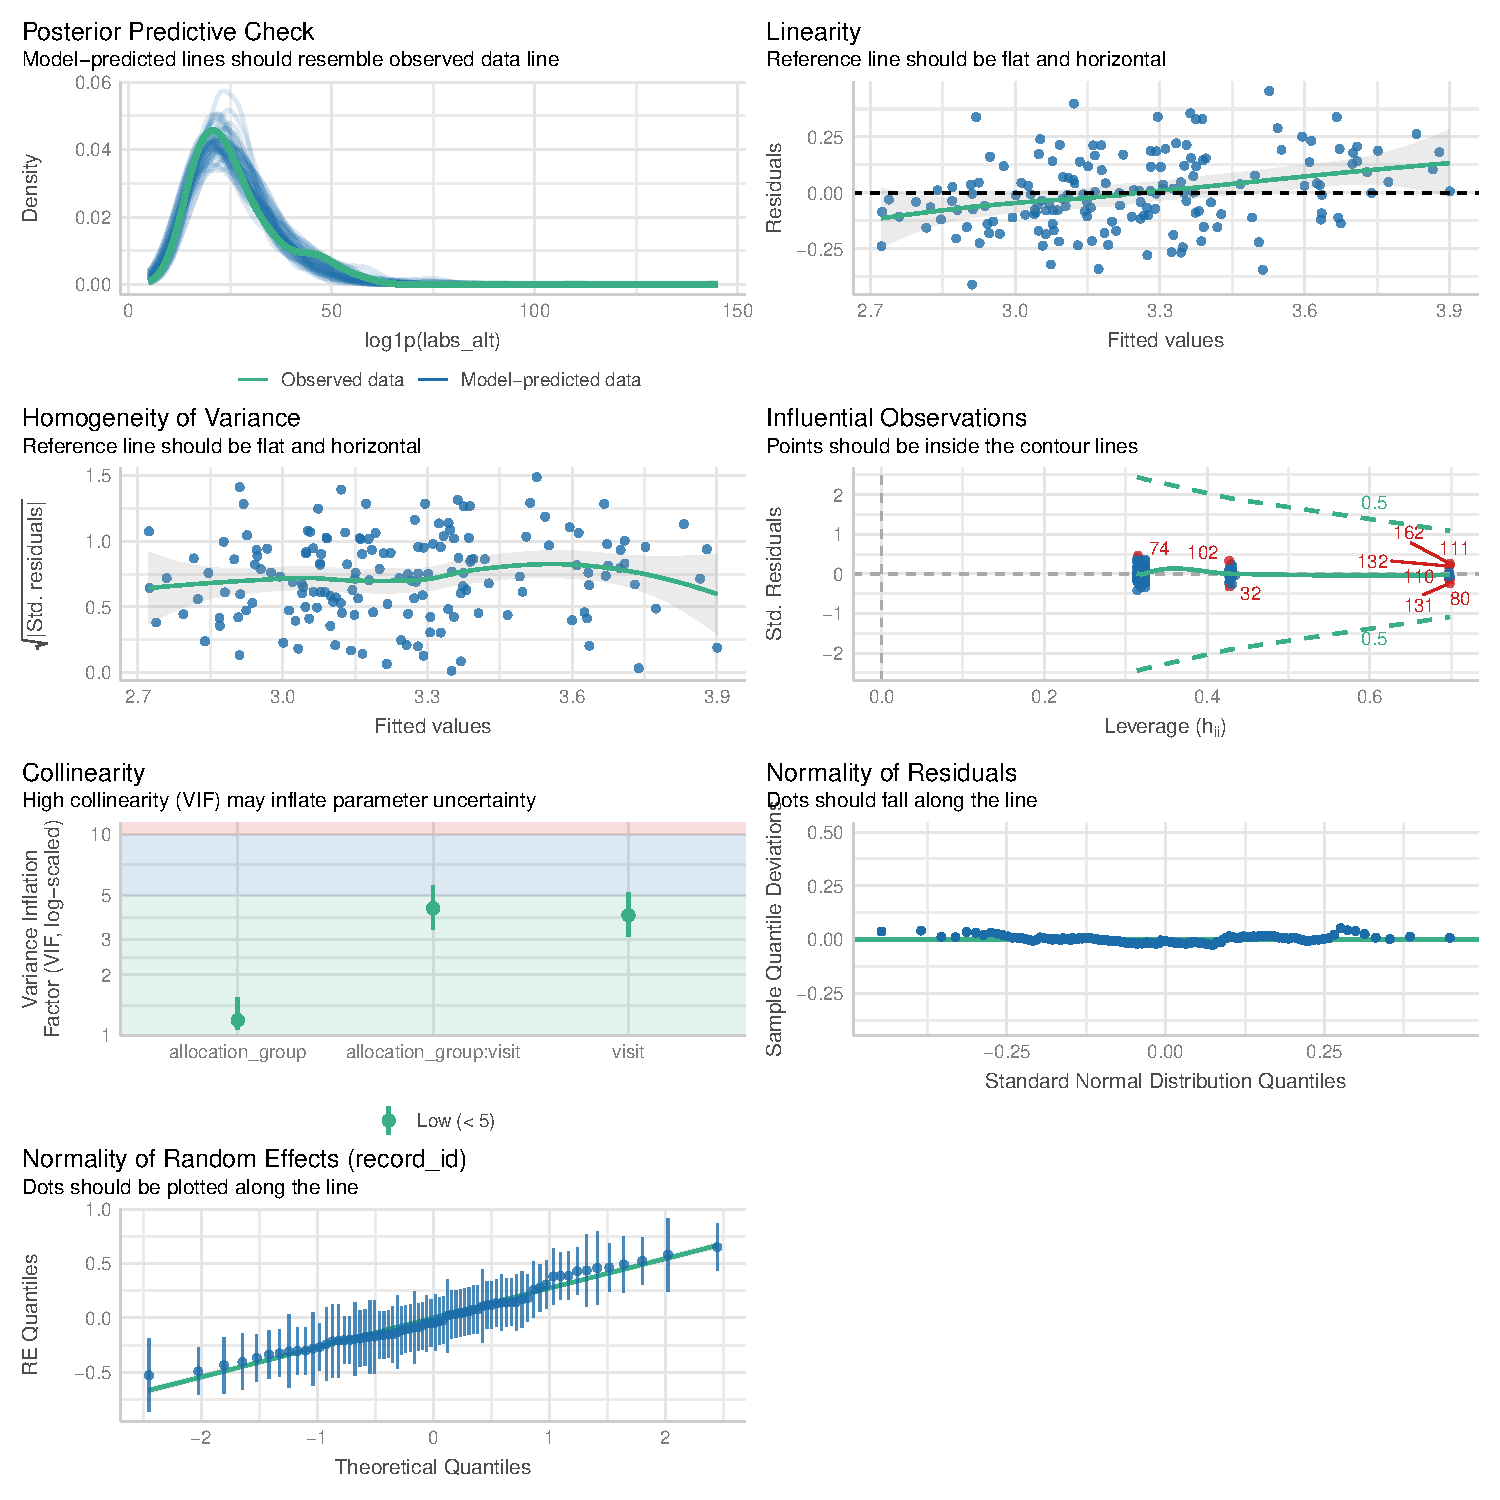
\includegraphics{Outcomes_files/figure-pdf/labs_alt_4-2.pdf}

\paragraph{Médias Marginais
Estimadas}\label{muxe9dias-marginais-estimadas-1}

\subparagraph{Todos os dados}\label{todos-os-dados-1}

\begin{Shaded}
\begin{Highlighting}[]
\CommentTok{\# Get EMMs for each group at each visit}
\NormalTok{labs\_alt\_raw\_emm }\OtherTok{\textless{}{-}}\NormalTok{ emmeans}\SpecialCharTok{::}\FunctionTok{emmeans}\NormalTok{(}
\NormalTok{    labs\_alt\_model, }
    \SpecialCharTok{\textasciitilde{}}\NormalTok{ allocation\_group }\SpecialCharTok{*}\NormalTok{ visit}
\NormalTok{)}

\NormalTok{labs\_alt\_raw\_emm }\OtherTok{\textless{}{-}} \FunctionTok{regrid}\NormalTok{(labs\_alt\_raw\_emm)}

\CommentTok{\# Table of marginal means}
\CommentTok{\# labs\_alt\_raw\_emm}

\CommentTok{\# Pairwise comparisons: Between groups at each visit}
\NormalTok{emmeans}\SpecialCharTok{::}\FunctionTok{contrast}\NormalTok{(labs\_alt\_raw\_emm,}
\AttributeTok{method =} \StringTok{"pairwise"}\NormalTok{, }\AttributeTok{by =} \StringTok{"visit"}\NormalTok{,}
\AttributeTok{adjust =} \StringTok{"bonferroni"}\NormalTok{) }\SpecialCharTok{\%\textgreater{}\%} \FunctionTok{summary}\NormalTok{(}\AttributeTok{infer =} \FunctionTok{c}\NormalTok{(}\ConstantTok{TRUE}\NormalTok{, }\ConstantTok{TRUE}\NormalTok{))}
\end{Highlighting}
\end{Shaded}

\begin{verbatim}
visit = 1:
 contrast          estimate   SE  df lower.CL upper.CL t.ratio p.value
 Grupo A - Grupo B    2.734 2.51 104    -2.25     7.72   1.088  0.2792

visit = 2:
 contrast          estimate   SE  df lower.CL upper.CL t.ratio p.value
 Grupo A - Grupo B    1.033 2.59 118    -4.10     6.16   0.399  0.6907

visit = 3:
 contrast          estimate   SE  df lower.CL upper.CL t.ratio p.value
 Grupo A - Grupo B    0.612 2.88 134    -5.09     6.32   0.212  0.8324

Degrees-of-freedom method: inherited from kenward-roger when re-gridding 
Confidence level used: 0.95 
\end{verbatim}

\begin{Shaded}
\begin{Highlighting}[]
\CommentTok{\# Pairwise comparisons: Changes over time within each group}
\NormalTok{emmeans}\SpecialCharTok{::}\FunctionTok{contrast}\NormalTok{(labs\_alt\_raw\_emm,}
\AttributeTok{method =} \StringTok{"pairwise"}\NormalTok{, }\AttributeTok{by =} \StringTok{"allocation\_group"}\NormalTok{,}
\AttributeTok{adjust =} \StringTok{"bonferroni"}\NormalTok{) }\SpecialCharTok{\%\textgreater{}\%} \FunctionTok{summary}\NormalTok{(}\AttributeTok{infer =} \FunctionTok{c}\NormalTok{(}\ConstantTok{TRUE}\NormalTok{, }\ConstantTok{TRUE}\NormalTok{))}
\end{Highlighting}
\end{Shaded}

\begin{verbatim}
allocation_group = Grupo A:
 contrast        estimate   SE  df lower.CL upper.CL t.ratio p.value
 visit1 - visit2    2.159 1.59 104    -1.71     6.03   1.357  0.5332
 visit1 - visit3    0.934 1.76 104    -3.35     5.21   0.531  1.0000
 visit2 - visit3   -1.225 1.72 118    -5.41     2.96  -0.711  1.0000

allocation_group = Grupo B:
 contrast        estimate   SE  df lower.CL upper.CL t.ratio p.value
 visit1 - visit2    0.458 1.59 104    -3.41     4.32   0.288  1.0000
 visit1 - visit3   -1.189 1.77 104    -5.49     3.11  -0.672  1.0000
 visit2 - visit3   -1.647 1.83 134    -6.07     2.78  -0.902  1.0000

Degrees-of-freedom method: inherited from kenward-roger when re-gridding 
Confidence level used: 0.95 
Conf-level adjustment: bonferroni method for 3 estimates 
P value adjustment: bonferroni method for 3 tests 
\end{verbatim}

\begin{Shaded}
\begin{Highlighting}[]
\CommentTok{\# Plot of marginal means}
\FunctionTok{plot}\NormalTok{(labs\_alt\_raw\_emm, }\AttributeTok{comparisons =} \ConstantTok{TRUE}\NormalTok{)}
\end{Highlighting}
\end{Shaded}

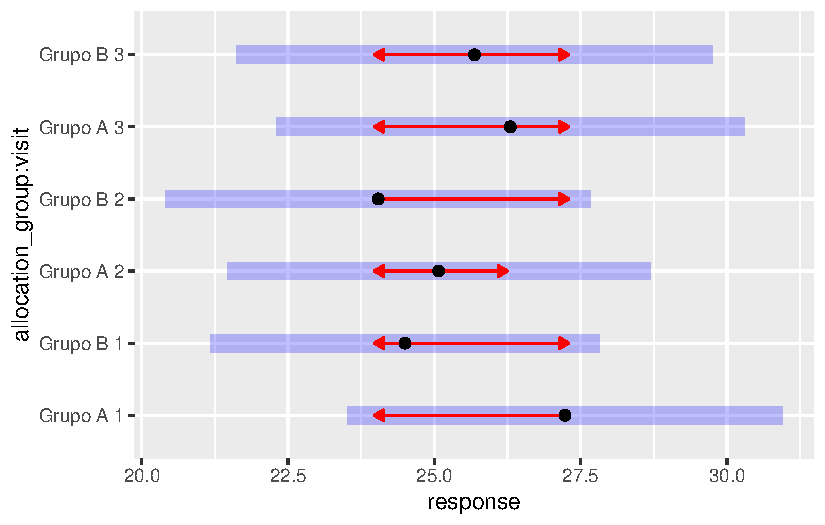
\includegraphics{Outcomes_files/figure-pdf/labs_alt_raw_emm-1.pdf}

\subparagraph{Análise de
sensibilidade}\label{anuxe1lise-de-sensibilidade-1}

\begin{Shaded}
\begin{Highlighting}[]
\CommentTok{\# Get EMMs for each group at each visit (Sensitivity Analysis)}
\NormalTok{labs\_alt\_emm }\OtherTok{\textless{}{-}}\NormalTok{ emmeans}\SpecialCharTok{::}\FunctionTok{emmeans}\NormalTok{(}
\NormalTok{    labs\_alt\_model\_sens, }
    \SpecialCharTok{\textasciitilde{}}\NormalTok{ allocation\_group }\SpecialCharTok{*}\NormalTok{ visit}
\NormalTok{)}

\NormalTok{labs\_alt\_emm }\OtherTok{\textless{}{-}} \FunctionTok{regrid}\NormalTok{(labs\_alt\_emm)}

\CommentTok{\# Table of marginal means}
\CommentTok{\# labs\_alt\_emm}

\CommentTok{\# Pairwise comparisons: Between groups at each visit}
\NormalTok{emmeans}\SpecialCharTok{::}\FunctionTok{contrast}\NormalTok{(labs\_alt\_emm,}
\AttributeTok{method =} \StringTok{"pairwise"}\NormalTok{, }\AttributeTok{by =} \StringTok{"visit"}\NormalTok{,}
\AttributeTok{adjust =} \StringTok{"bonferroni"}\NormalTok{) }\SpecialCharTok{\%\textgreater{}\%} \FunctionTok{summary}\NormalTok{(}\AttributeTok{infer =} \FunctionTok{c}\NormalTok{(}\ConstantTok{TRUE}\NormalTok{, }\ConstantTok{TRUE}\NormalTok{))}
\end{Highlighting}
\end{Shaded}

\begin{verbatim}
visit = 1:
 contrast          estimate   SE    df lower.CL upper.CL t.ratio p.value
 Grupo A - Grupo B    0.335 2.27  93.7    -4.16     4.83   0.148  0.8827

visit = 2:
 contrast          estimate   SE    df lower.CL upper.CL t.ratio p.value
 Grupo A - Grupo B    0.558 2.38 107.7    -4.17     5.28   0.234  0.8153

visit = 3:
 contrast          estimate   SE    df lower.CL upper.CL t.ratio p.value
 Grupo A - Grupo B   -0.770 2.56 125.2    -5.84     4.31  -0.300  0.7645

Degrees-of-freedom method: inherited from kenward-roger when re-gridding 
Confidence level used: 0.95 
\end{verbatim}

\begin{Shaded}
\begin{Highlighting}[]
\CommentTok{\# Pairwise comparisons: Changes over time within each group}
\NormalTok{emmeans}\SpecialCharTok{::}\FunctionTok{contrast}\NormalTok{(labs\_alt\_emm,}
\AttributeTok{method =} \StringTok{"pairwise"}\NormalTok{, }\AttributeTok{by =} \StringTok{"allocation\_group"}\NormalTok{,}
\AttributeTok{adjust =} \StringTok{"bonferroni"}\NormalTok{) }\SpecialCharTok{\%\textgreater{}\%} \FunctionTok{summary}\NormalTok{(}\AttributeTok{infer =} \FunctionTok{c}\NormalTok{(}\ConstantTok{TRUE}\NormalTok{, }\ConstantTok{TRUE}\NormalTok{))}
\end{Highlighting}
\end{Shaded}

\begin{verbatim}
allocation_group = Grupo A:
 contrast        estimate   SE    df lower.CL upper.CL t.ratio p.value
 visit1 - visit2    0.549 1.41  93.7    -2.88     3.98   0.390  1.0000
 visit1 - visit3    0.897 1.53  93.7    -2.84     4.63   0.586  1.0000
 visit2 - visit3    0.348 1.54 107.7    -3.39     4.09   0.226  1.0000

allocation_group = Grupo B:
 contrast        estimate   SE    df lower.CL upper.CL t.ratio p.value
 visit1 - visit2    0.772 1.39  93.7    -2.62     4.16   0.555  1.0000
 visit1 - visit3   -0.207 1.55  93.7    -3.98     3.56  -0.134  1.0000
 visit2 - visit3   -0.980 1.57 118.5    -4.80     2.84  -0.622  1.0000

Degrees-of-freedom method: inherited from kenward-roger when re-gridding 
Confidence level used: 0.95 
Conf-level adjustment: bonferroni method for 3 estimates 
P value adjustment: bonferroni method for 3 tests 
\end{verbatim}

\begin{Shaded}
\begin{Highlighting}[]
\CommentTok{\# Plot of marginal means}
\FunctionTok{plot}\NormalTok{(labs\_alt\_emm, }\AttributeTok{comparisons =} \ConstantTok{TRUE}\NormalTok{)}
\end{Highlighting}
\end{Shaded}

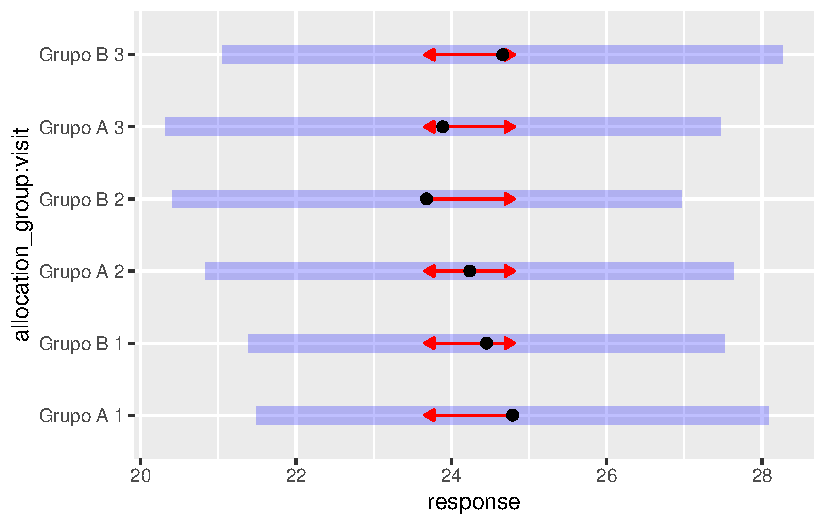
\includegraphics{Outcomes_files/figure-pdf/labs_alt_sens_emm-1.pdf}

\paragraph{Resultado}\label{resultado-1}

No modelo ajustado para os níveis de ALT, não foram observadas
diferenças estatisticamente significativas entre os grupos em nenhum dos
três momentos avaliados. Da mesma forma, não houve mudanças
significativas ao longo do tempo dentro de cada grupo. A análise de
sensibilidade, realizada com a exclusão das observações influentes,
confirmou esses achados. As estimativas permaneceram estáveis e todas as
comparações entre os grupos e ao longo do tempo mantiveram-se não
significativas. As estimativas, intervalos de confiança de 95\% e
valores de p estão apresentados na Tabela~\ref{tbl-alt}.

\begin{longtable}[]{@{}
  >{\raggedright\arraybackslash}p{(\columnwidth - 8\tabcolsep) * \real{0.2000}}
  >{\raggedright\arraybackslash}p{(\columnwidth - 8\tabcolsep) * \real{0.2000}}
  >{\raggedright\arraybackslash}p{(\columnwidth - 8\tabcolsep) * \real{0.2000}}
  >{\raggedright\arraybackslash}p{(\columnwidth - 8\tabcolsep) * \real{0.2000}}
  >{\raggedright\arraybackslash}p{(\columnwidth - 8\tabcolsep) * \real{0.2000}}@{}}
\caption{Diferenças estimadas dos níveis de Alanina Aminotransferase
(ALT) entre os grupos de alocação (placebo vs Eclipta) e entre visitas
dentro de cada grupo}\label{tbl-alt}\tabularnewline
\toprule\noalign{}
\begin{minipage}[b]{\linewidth}\raggedright
Grupo de comparação
\end{minipage} & \begin{minipage}[b]{\linewidth}\raggedright
Comparação
\end{minipage} & \begin{minipage}[b]{\linewidth}\raggedright
Estimativa
\end{minipage} & \begin{minipage}[b]{\linewidth}\raggedright
IC 95\%
\end{minipage} & \begin{minipage}[b]{\linewidth}\raggedright
p-valor
\end{minipage} \\
\midrule\noalign{}
\endfirsthead
\toprule\noalign{}
\begin{minipage}[b]{\linewidth}\raggedright
Grupo de comparação
\end{minipage} & \begin{minipage}[b]{\linewidth}\raggedright
Comparação
\end{minipage} & \begin{minipage}[b]{\linewidth}\raggedright
Estimativa
\end{minipage} & \begin{minipage}[b]{\linewidth}\raggedright
IC 95\%
\end{minipage} & \begin{minipage}[b]{\linewidth}\raggedright
p-valor
\end{minipage} \\
\midrule\noalign{}
\endhead
\bottomrule\noalign{}
\endlastfoot
Entre grupos & Visita 1 & 2,73 & {[}-2,25 ; 7,72{]} & 0,279 \\
Entre grupos & Visita 2 & 1,03 & {[}-4,10 ; 6,16{]} & 0,691 \\
Entre grupos & Visita 3 & 0,61 & {[}-5,09 ; 6,32{]} & 0,832 \\
Grupo Placebo & Visita 1 - Visita 2 & 2,16 & {[}-1,71 ; 6,03{]} &
0,533 \\
Grupo Placebo & Visita 1 - Visita 3 & 0,93 & {[}-3,35 ; 5,21{]} &
1,000 \\
Grupo Placebo & Visita 2 - Visita 3 & -1,23 & {[}-5,41 ; 2,96{]} &
1,000 \\
Grupo Eclipta & Visita 1 - Visita 2 & 0,46 & {[}-3,41 ; 4,32{]} &
1,000 \\
Grupo Eclipta & Visita 1 - Visita 3 & -1,19 & {[}-5,49 ; 3,11{]} &
1,000 \\
Grupo Eclipta & Visita 2 - Visita 3 & -1,65 & {[}-6,07 ; 2,78{]} &
1,000 \\
\end{longtable}

\begin{Shaded}
\begin{Highlighting}[]
\FunctionTok{ggplot}\NormalTok{(}
    \AttributeTok{data =}\NormalTok{ data\_model, }
    \FunctionTok{aes}\NormalTok{(}
        \AttributeTok{x =} \FunctionTok{as.factor}\NormalTok{(visit),}
        \AttributeTok{y =}\NormalTok{ labs\_alt,}
        \AttributeTok{group =}\NormalTok{ record\_id,}
\NormalTok{    )}
\NormalTok{) }\SpecialCharTok{+}
    \FunctionTok{geom\_line}\NormalTok{(}\AttributeTok{alpha =} \FloatTok{0.5}\NormalTok{) }\SpecialCharTok{+}
    \FunctionTok{geom\_point}\NormalTok{(}\AttributeTok{alpha =} \FloatTok{0.7}\NormalTok{) }\SpecialCharTok{+}
    \FunctionTok{geom\_smooth}\NormalTok{(}
        \FunctionTok{aes}\NormalTok{(}\AttributeTok{group =}\NormalTok{ allocation\_group),}
        \AttributeTok{method =} \StringTok{"lm"}\NormalTok{,}
        \AttributeTok{se =} \ConstantTok{TRUE}\NormalTok{,}
        \AttributeTok{linewidth =} \DecValTok{1}
\NormalTok{    ) }\SpecialCharTok{+}
    \FunctionTok{labs}\NormalTok{(}\AttributeTok{title =} \StringTok{"All data"}\NormalTok{) }\SpecialCharTok{+}
    \FunctionTok{facet\_wrap}\NormalTok{(}\SpecialCharTok{\textasciitilde{}}\NormalTok{ allocation\_group) }\SpecialCharTok{+} 
    \FunctionTok{coord\_cartesian}\NormalTok{(}\AttributeTok{ylim =} \FunctionTok{c}\NormalTok{(}\DecValTok{10}\NormalTok{, }\DecValTok{80}\NormalTok{))}
\end{Highlighting}
\end{Shaded}

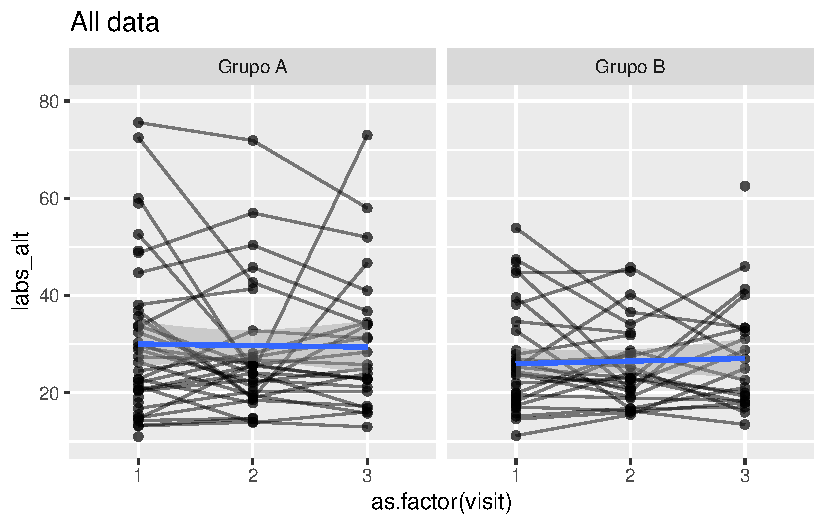
\includegraphics{Outcomes_files/figure-pdf/labs_alt_6-1.pdf}

\begin{Shaded}
\begin{Highlighting}[]
\NormalTok{data\_model }\SpecialCharTok{\%\textgreater{}\%} 
    \FunctionTok{filter}\NormalTok{(}
        \SpecialCharTok{!}\NormalTok{(record\_id }\SpecialCharTok{\%in\%} 
\NormalTok{        labs\_alt\_model\_check}\SpecialCharTok{$}\NormalTok{influential\_ids)}
\NormalTok{    ) }\SpecialCharTok{\%\textgreater{}\%} 
    \FunctionTok{ggplot}\NormalTok{(}
        \FunctionTok{aes}\NormalTok{(}
            \AttributeTok{x =} \FunctionTok{as.factor}\NormalTok{(visit),}
            \AttributeTok{y =}\NormalTok{ labs\_alt,}
            \AttributeTok{group =}\NormalTok{ record\_id,}
\NormalTok{        )}
\NormalTok{    ) }\SpecialCharTok{+}
    \FunctionTok{geom\_line}\NormalTok{(}\AttributeTok{alpha =} \FloatTok{0.5}\NormalTok{) }\SpecialCharTok{+}
    \FunctionTok{geom\_point}\NormalTok{(}\AttributeTok{alpha =} \FloatTok{0.7}\NormalTok{) }\SpecialCharTok{+}
    \FunctionTok{geom\_smooth}\NormalTok{(}
        \FunctionTok{aes}\NormalTok{(}\AttributeTok{group =}\NormalTok{ allocation\_group),}
        \AttributeTok{method =} \StringTok{"lm"}\NormalTok{,}
        \AttributeTok{se =} \ConstantTok{TRUE}\NormalTok{,}
        \AttributeTok{linewidth =} \DecValTok{1}
\NormalTok{    ) }\SpecialCharTok{+}
    \FunctionTok{labs}\NormalTok{(}\AttributeTok{title =} \StringTok{"Sensitivity analysis"}\NormalTok{) }\SpecialCharTok{+}
    \FunctionTok{facet\_wrap}\NormalTok{(}\SpecialCharTok{\textasciitilde{}}\NormalTok{ allocation\_group) }\SpecialCharTok{+} 
    \FunctionTok{coord\_cartesian}\NormalTok{(}\AttributeTok{ylim =} \FunctionTok{c}\NormalTok{(}\DecValTok{10}\NormalTok{, }\DecValTok{80}\NormalTok{))}
\end{Highlighting}
\end{Shaded}

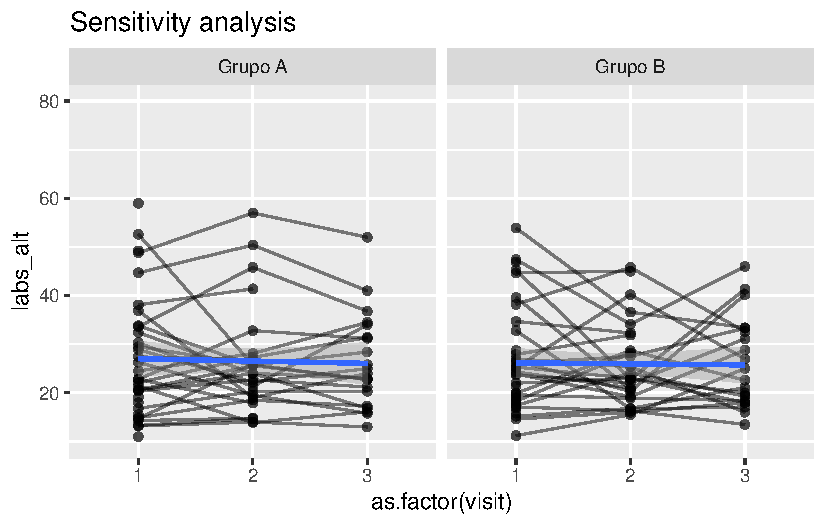
\includegraphics{Outcomes_files/figure-pdf/labs_alt_6-2.pdf}

\subsubsection{Gama
Glutamil-transferase}\label{gama-glutamil-transferase}

Variável: \texttt{labs\_ggt}

\begin{Shaded}
\begin{Highlighting}[]
\CommentTok{\# Plot 1: Raw data}
\NormalTok{labs\_ggt\_hist\_1 }\OtherTok{\textless{}{-}}\NormalTok{ data\_model }\SpecialCharTok{\%\textgreater{}\%} 
    \FunctionTok{filter}\NormalTok{(}
\NormalTok{        labs\_ggt }\SpecialCharTok{\textless{}} \DecValTok{300}
\NormalTok{    ) }\SpecialCharTok{\%\textgreater{}\%} 
    \FunctionTok{ggplot}\NormalTok{(}\FunctionTok{aes}\NormalTok{(}\AttributeTok{x =}\NormalTok{ labs\_ggt)) }\SpecialCharTok{+} 
    \FunctionTok{geom\_histogram}\NormalTok{(}\AttributeTok{bins =} \DecValTok{50}\NormalTok{, }\AttributeTok{fill =} \StringTok{"skyblue"}\NormalTok{, }\AttributeTok{color =} \StringTok{"black"}\NormalTok{)}

\CommentTok{\# Plot 2: Log{-}transformed data}
\NormalTok{labs\_ggt\_hist\_2 }\OtherTok{\textless{}{-}}\NormalTok{ data\_model }\SpecialCharTok{\%\textgreater{}\%} 
    \FunctionTok{filter}\NormalTok{(}
\NormalTok{        labs\_ggt }\SpecialCharTok{\textless{}} \DecValTok{300}
\NormalTok{    ) }\SpecialCharTok{\%\textgreater{}\%}
    \FunctionTok{ggplot}\NormalTok{(}\FunctionTok{aes}\NormalTok{(}\AttributeTok{x =} \FunctionTok{log1p}\NormalTok{(labs\_ggt))) }\SpecialCharTok{+} 
    \FunctionTok{geom\_histogram}\NormalTok{(}\AttributeTok{bins =} \DecValTok{50}\NormalTok{, }\AttributeTok{fill =} \StringTok{"lightgreen"}\NormalTok{, }\AttributeTok{color =} \StringTok{"black"}\NormalTok{)}

\CommentTok{\# Combine side by side}
\NormalTok{labs\_ggt\_hist\_1 }\SpecialCharTok{+}\NormalTok{ labs\_ggt\_hist\_2 }\CommentTok{\# library(patchwork)}
\end{Highlighting}
\end{Shaded}

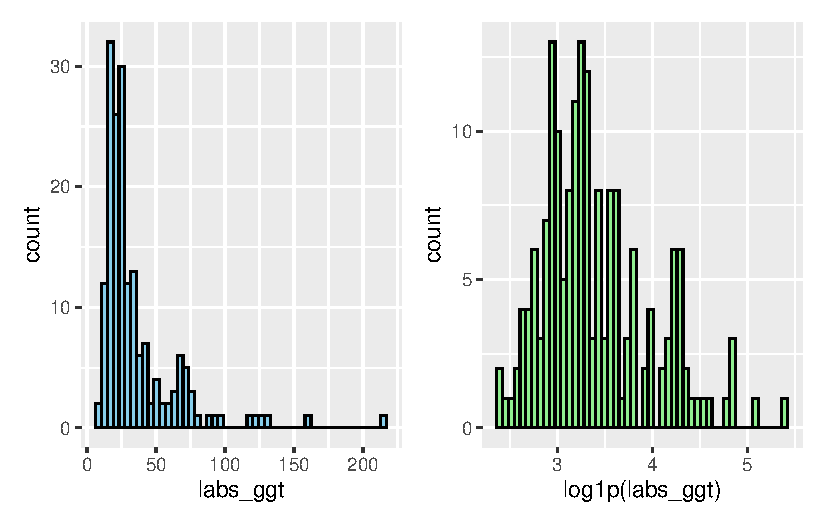
\includegraphics{Outcomes_files/figure-pdf/labs_ggt_1-1.pdf}

\begin{Shaded}
\begin{Highlighting}[]
\CommentTok{\# LMM}
\NormalTok{labs\_ggt\_model }\OtherTok{\textless{}{-}} \FunctionTok{lmer}\NormalTok{(}\FunctionTok{log1p}\NormalTok{(labs\_ggt) }\SpecialCharTok{\textasciitilde{}}\NormalTok{ allocation\_group }\SpecialCharTok{*}\NormalTok{ visit }\SpecialCharTok{+} 
\NormalTok{(}\DecValTok{1} \SpecialCharTok{|}\NormalTok{ record\_id), }\AttributeTok{data =}\NormalTok{ data\_model)}
\FunctionTok{check\_collinearity}\NormalTok{(labs\_ggt\_model)}
\end{Highlighting}
\end{Shaded}

\begin{verbatim}
# Check for Multicollinearity

Low Correlation

                   Term  VIF   VIF 95% CI Increased SE Tolerance Tolerance 95% CI
       allocation_group 1.08 [1.01, 1.64]         1.04      0.93     [0.61, 0.99]
                  visit 3.40 [2.71, 4.36]         1.84      0.29     [0.23, 0.37]
 allocation_group:visit 3.51 [2.79, 4.51]         1.87      0.28     [0.22, 0.36]
\end{verbatim}

\begin{Shaded}
\begin{Highlighting}[]
\CommentTok{\# Sensitivity analysis}
\NormalTok{labs\_ggt\_model\_check }\OtherTok{\textless{}{-}} \FunctionTok{sensitivity\_check\_lmer}\NormalTok{(}
    \AttributeTok{model =}\NormalTok{ labs\_ggt\_model,}
    \AttributeTok{id\_var =} \StringTok{"record\_id"}\NormalTok{,}
    \AttributeTok{top\_n =} \DecValTok{7}\NormalTok{)}

\CommentTok{\# LMM Sensitivity}
\NormalTok{labs\_ggt\_model\_sens }\OtherTok{\textless{}{-}} \FunctionTok{update}\NormalTok{(}\AttributeTok{object =}\NormalTok{ labs\_ggt\_model,}
                              \AttributeTok{subset =} \SpecialCharTok{!}\NormalTok{(record\_id }\SpecialCharTok{\%in\%} 
\NormalTok{        labs\_ggt\_model\_check}\SpecialCharTok{$}\NormalTok{influential\_ids))}
\CommentTok{\# Influential IDS}
\NormalTok{labs\_ggt\_model\_check}\SpecialCharTok{$}\NormalTok{influential\_ids}
\end{Highlighting}
\end{Shaded}

\begin{verbatim}
[1] "13" "46" "49" "58" "22" "34" "41"
\end{verbatim}

\paragraph{Resumo dos modelos}\label{resumo-dos-modelos-2}

\begin{Shaded}
\begin{Highlighting}[]
\CommentTok{\# Model comparison}
\FunctionTok{summary}\NormalTok{(labs\_ggt\_model)}
\end{Highlighting}
\end{Shaded}

\begin{verbatim}
Linear mixed model fit by REML. t-tests use Satterthwaite's method ['lmerModLmerTest']
Formula: log1p(labs_ggt) ~ allocation_group * visit + (1 | record_id)
   Data: data_model

REML criterion at convergence: 214.3

Scaled residuals: 
     Min       1Q   Median       3Q      Max 
-1.98517 -0.41941 -0.02504  0.42332  2.68048 

Random effects:
 Groups    Name        Variance Std.Dev.
 record_id (Intercept) 0.35840  0.5987  
 Residual              0.05825  0.2413  
Number of obs: 178, groups:  record_id, 75

Fixed effects:
                               Estimate Std. Error       df t value Pr(>|t|)    
(Intercept)                     3.36365    0.10612 81.55575  31.697   <2e-16 ***
allocation_groupGrupo B         0.05279    0.14908 81.55575   0.354    0.724    
visit2                         -0.02673    0.06095 98.79849  -0.439    0.662    
visit3                          0.01219    0.06614 99.26017   0.184    0.854    
allocation_groupGrupo B:visit2  0.04689    0.08964 99.59537   0.523    0.602    
allocation_groupGrupo B:visit3  0.02698    0.09736 99.95801   0.277    0.782    
---
Signif. codes:  0 '***' 0.001 '**' 0.01 '*' 0.05 '.' 0.1 ' ' 1

Correlation of Fixed Effects:
            (Intr) all_GB visit2 visit3 a_GB:2
allctn_grGB -0.712                            
visit2      -0.243  0.173                     
visit3      -0.224  0.160  0.455              
allctn_GB:2  0.166 -0.233 -0.680 -0.310       
allctn_GB:3  0.152 -0.214 -0.309 -0.679  0.436
\end{verbatim}

\begin{Shaded}
\begin{Highlighting}[]
\FunctionTok{summary}\NormalTok{(labs\_ggt\_model\_sens)}
\end{Highlighting}
\end{Shaded}

\begin{verbatim}
Linear mixed model fit by REML. t-tests use Satterthwaite's method ['lmerModLmerTest']
Formula: log1p(labs_ggt) ~ allocation_group * visit + (1 | record_id)
   Data: data_model
 Subset: !(record_id %in% labs_ggt_model_check$influential_ids)

REML criterion at convergence: 129.2

Scaled residuals: 
     Min       1Q   Median       3Q      Max 
-2.06521 -0.44956 -0.01804  0.45494  1.81501 

Random effects:
 Groups    Name        Variance Std.Dev.
 record_id (Intercept) 0.2520   0.5020  
 Residual              0.0364   0.1908  
Number of obs: 160, groups:  record_id, 68

Fixed effects:
                               Estimate Std. Error       df t value Pr(>|t|)    
(Intercept)                     3.21202    0.09349 74.25204  34.357   <2e-16 ***
allocation_groupGrupo B         0.14499    0.13031 74.25204   1.113    0.269    
visit2                         -0.01105    0.05075 89.14440  -0.218    0.828    
visit3                          0.03893    0.05564 89.56439   0.700    0.486    
allocation_groupGrupo B:visit2  0.06129    0.07498 89.97944   0.817    0.416    
allocation_groupGrupo B:visit3  0.01693    0.08145 90.24696   0.208    0.836    
---
Signif. codes:  0 '***' 0.001 '**' 0.01 '*' 0.05 '.' 0.1 ' ' 1

Correlation of Fixed Effects:
            (Intr) all_GB visit2 visit3 a_GB:2
allctn_grGB -0.717                            
visit2      -0.233  0.167                     
visit3      -0.212  0.152  0.452              
allctn_GB:2  0.157 -0.219 -0.677 -0.306       
allctn_GB:3  0.145 -0.202 -0.309 -0.683  0.434
\end{verbatim}

\begin{Shaded}
\begin{Highlighting}[]
\NormalTok{labs\_ggt\_model\_check}\SpecialCharTok{$}\NormalTok{comparison\_table}
\end{Highlighting}
\end{Shaded}

\begin{verbatim}
# A tibble: 16 x 6
   Model       term                           estimate std.error statistic   p.value
   <chr>       <chr>                             <dbl>     <dbl>     <dbl>     <dbl>
 1 Original    (Intercept)                      3.36      0.106     31.7    1.28e-47
 2 Sensitivity (Intercept)                      3.21      0.0935    34.4    2.48e-47
 3 Original    allocation_groupGrupo B          0.0528    0.149      0.354  7.24e- 1
 4 Sensitivity allocation_groupGrupo B          0.145     0.130      1.11   2.69e- 1
 5 Original    allocation_groupGrupo B:visit2   0.0469    0.0896     0.523  6.02e- 1
 6 Sensitivity allocation_groupGrupo B:visit2   0.0613    0.0750     0.817  4.16e- 1
 7 Original    allocation_groupGrupo B:visit3   0.0270    0.0974     0.277  7.82e- 1
 8 Sensitivity allocation_groupGrupo B:visit3   0.0169    0.0814     0.208  8.36e- 1
 9 Original    sd__(Intercept)                  0.599    NA         NA     NA       
10 Sensitivity sd__(Intercept)                  0.502    NA         NA     NA       
11 Original    sd__Observation                  0.241    NA         NA     NA       
12 Sensitivity sd__Observation                  0.191    NA         NA     NA       
13 Original    visit2                          -0.0267    0.0610    -0.439  6.62e- 1
14 Sensitivity visit2                          -0.0110    0.0507    -0.218  8.28e- 1
15 Original    visit3                           0.0122    0.0661     0.184  8.54e- 1
16 Sensitivity visit3                           0.0389    0.0556     0.700  4.86e- 1
\end{verbatim}

\begin{Shaded}
\begin{Highlighting}[]
\NormalTok{performance}\SpecialCharTok{::}\FunctionTok{compare\_performance}\NormalTok{(}
\NormalTok{    labs\_ggt\_model, }
\NormalTok{    labs\_ggt\_model\_sens)}
\end{Highlighting}
\end{Shaded}

\begin{verbatim}
# Comparison of Model Performance Indices

Name                |           Model |  AIC (weights) | AICc (weights) |  BIC (weights) | R2 (cond.) | R2 (marg.) |   ICC |  RMSE | Sigma
------------------------------------------------------------------------------------------------------------------------------------------
labs_ggt_model      | lmerModLmerTest | 1425.1 (<.001) | 1426.0 (<.001) | 1450.6 (<.001) |      0.861 |      0.004 | 0.860 | 0.185 | 0.241
labs_ggt_model_sens | lmerModLmerTest | 1189.5 (>.999) | 1190.4 (>.999) | 1214.1 (>.999) |      0.877 |      0.026 | 0.874 | 0.145 | 0.191
\end{verbatim}

\begin{Shaded}
\begin{Highlighting}[]
\NormalTok{performance}\SpecialCharTok{::}\FunctionTok{check\_model}\NormalTok{(labs\_ggt\_model)}
\end{Highlighting}
\end{Shaded}

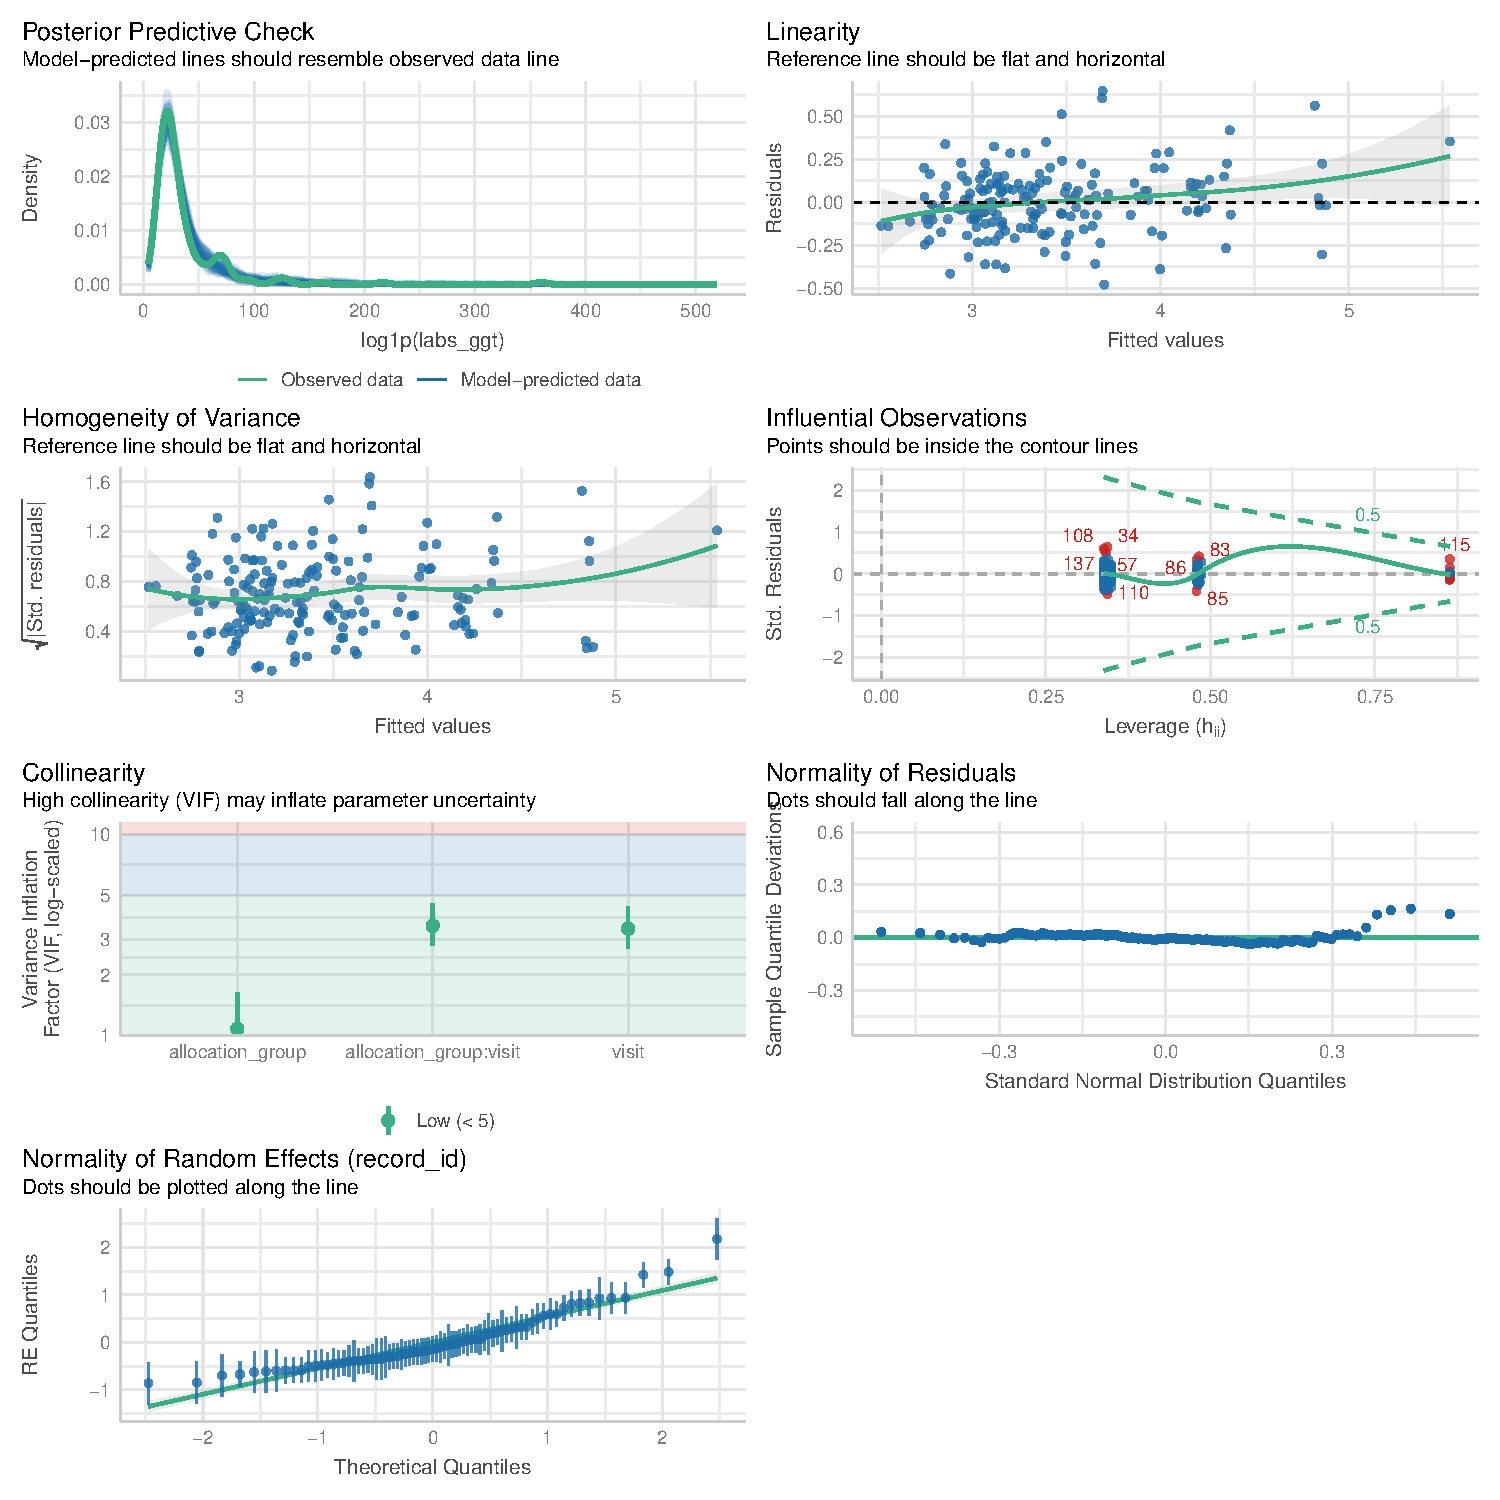
\includegraphics{Outcomes_files/figure-pdf/labs_ggt_4-1.pdf}

\begin{Shaded}
\begin{Highlighting}[]
\NormalTok{performance}\SpecialCharTok{::}\FunctionTok{check\_model}\NormalTok{(labs\_ggt\_model\_sens)}
\end{Highlighting}
\end{Shaded}

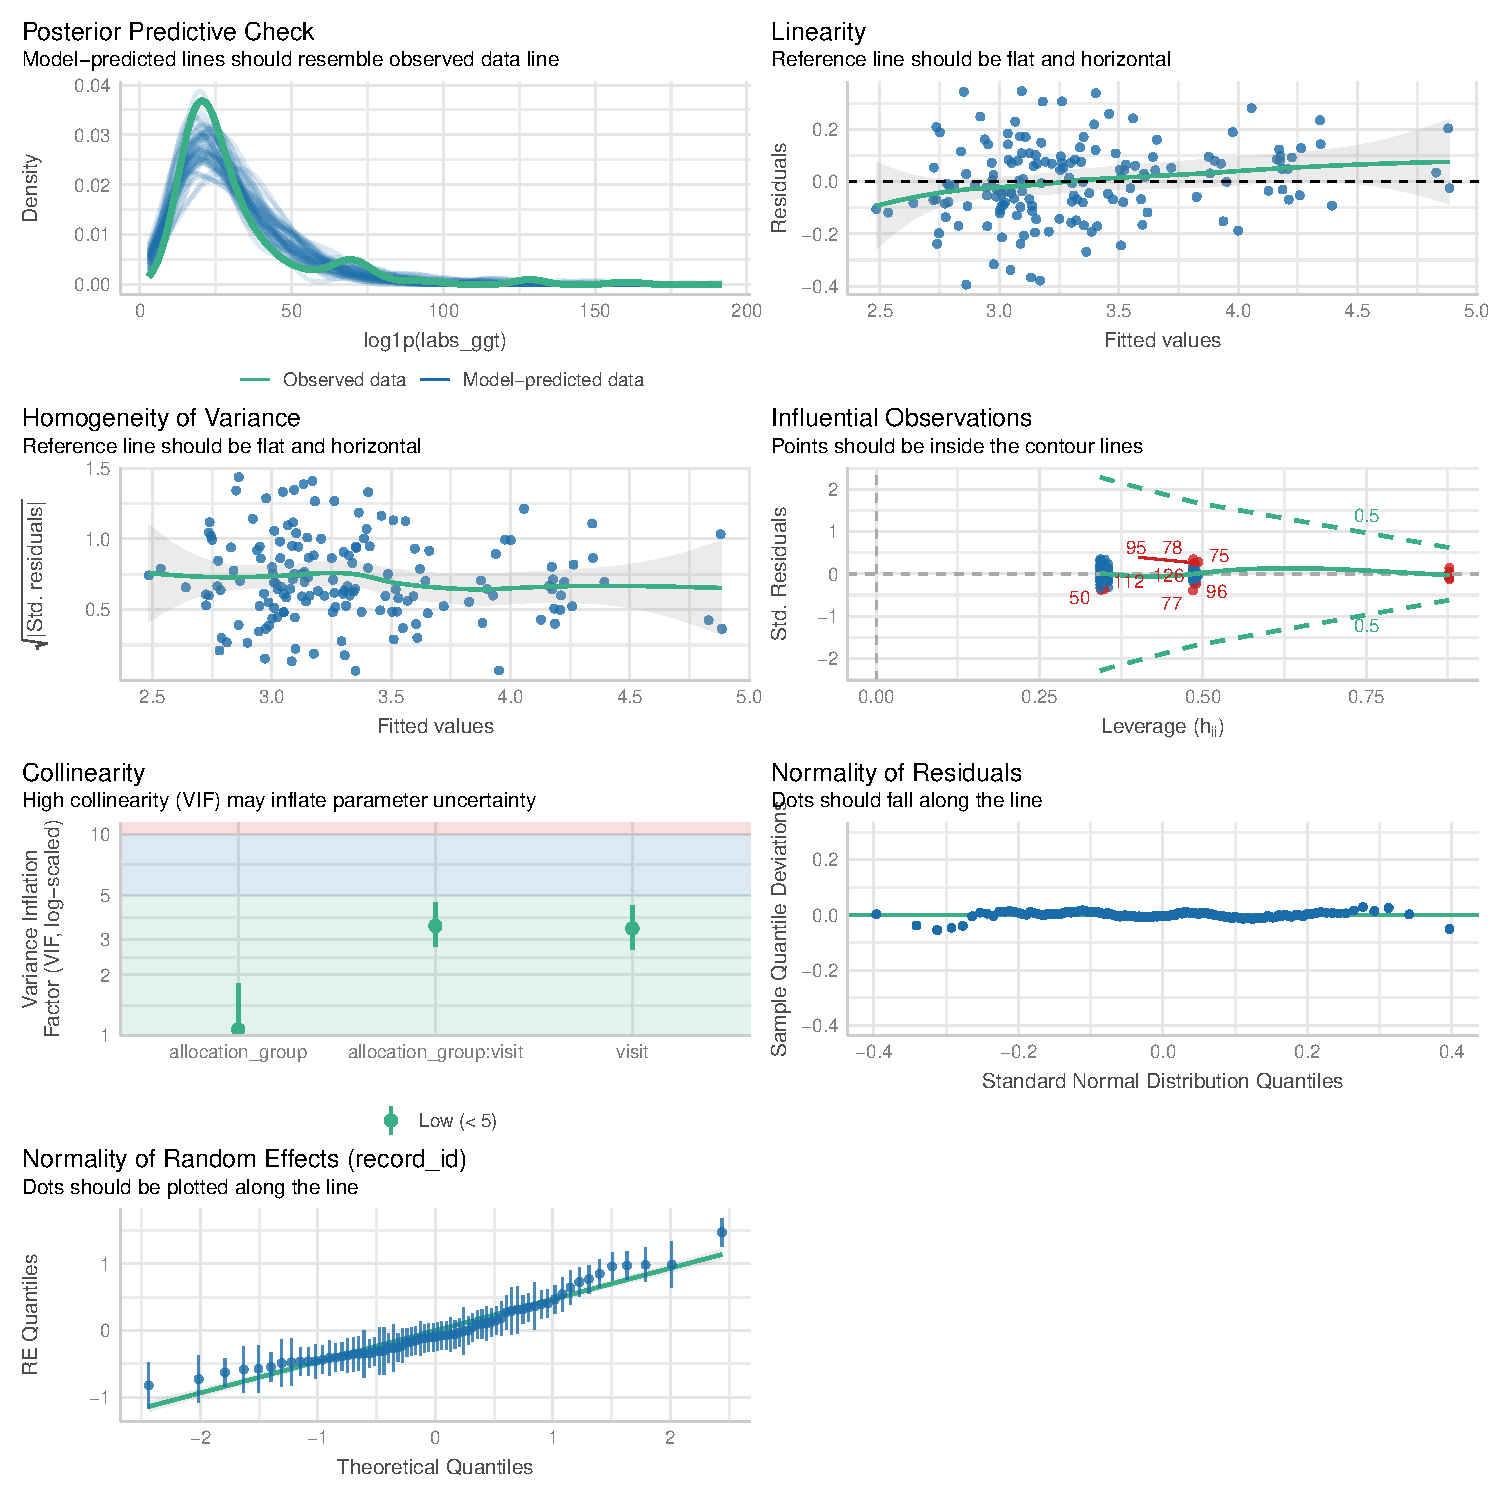
\includegraphics{Outcomes_files/figure-pdf/labs_ggt_4-2.pdf}

\paragraph{Médias Marginais
Estimadas}\label{muxe9dias-marginais-estimadas-2}

\subparagraph{Todos os dados}\label{todos-os-dados-2}

\begin{Shaded}
\begin{Highlighting}[]
\CommentTok{\# Get EMMs for each group at each visit}
\NormalTok{labs\_ggt\_raw\_emm }\OtherTok{\textless{}{-}}\NormalTok{ emmeans}\SpecialCharTok{::}\FunctionTok{emmeans}\NormalTok{(}
\NormalTok{    labs\_ggt\_model, }
    \SpecialCharTok{\textasciitilde{}}\NormalTok{ allocation\_group }\SpecialCharTok{*}\NormalTok{ visit}
\NormalTok{)}

\NormalTok{labs\_ggt\_raw\_emm }\OtherTok{\textless{}{-}} \FunctionTok{regrid}\NormalTok{(labs\_ggt\_raw\_emm)}

\CommentTok{\# Table of marginal means}
\CommentTok{\# labs\_ggt\_raw\_emm}

\CommentTok{\# Pairwise comparisons: Between groups at each visit}
\NormalTok{emmeans}\SpecialCharTok{::}\FunctionTok{contrast}\NormalTok{(labs\_ggt\_raw\_emm,}
\AttributeTok{method =} \StringTok{"pairwise"}\NormalTok{, }\AttributeTok{by =} \StringTok{"visit"}\NormalTok{,}
\AttributeTok{adjust =} \StringTok{"bonferroni"}\NormalTok{) }\SpecialCharTok{\%\textgreater{}\%} \FunctionTok{summary}\NormalTok{(}\AttributeTok{infer =} \FunctionTok{c}\NormalTok{(}\ConstantTok{TRUE}\NormalTok{, }\ConstantTok{TRUE}\NormalTok{))}
\end{Highlighting}
\end{Shaded}

\begin{verbatim}
visit = 1:
 contrast          estimate   SE    df lower.CL upper.CL t.ratio p.value
 Grupo A - Grupo B    -1.57 4.42  84.1    -10.4     7.23  -0.354  0.7242

visit = 2:
 contrast          estimate   SE    df lower.CL upper.CL t.ratio p.value
 Grupo A - Grupo B    -2.95 4.60  91.4    -12.1     6.19  -0.641  0.5232

visit = 3:
 contrast          estimate   SE    df lower.CL upper.CL t.ratio p.value
 Grupo A - Grupo B    -2.43 4.87 100.1    -12.1     7.24  -0.498  0.6193

Degrees-of-freedom method: inherited from kenward-roger when re-gridding 
Confidence level used: 0.95 
\end{verbatim}

\begin{Shaded}
\begin{Highlighting}[]
\CommentTok{\# Pairwise comparisons: Changes over time within each group}
\NormalTok{emmeans}\SpecialCharTok{::}\FunctionTok{contrast}\NormalTok{(labs\_ggt\_raw\_emm,}
\AttributeTok{method =} \StringTok{"pairwise"}\NormalTok{, }\AttributeTok{by =} \StringTok{"allocation\_group"}\NormalTok{,}
\AttributeTok{adjust =} \StringTok{"bonferroni"}\NormalTok{) }\SpecialCharTok{\%\textgreater{}\%} \FunctionTok{summary}\NormalTok{(}\AttributeTok{infer =} \FunctionTok{c}\NormalTok{(}\ConstantTok{TRUE}\NormalTok{, }\ConstantTok{TRUE}\NormalTok{))}
\end{Highlighting}
\end{Shaded}

\begin{verbatim}
allocation_group = Grupo A:
 contrast        estimate   SE    df lower.CL upper.CL t.ratio p.value
 visit1 - visit2    0.762 1.74  84.1    -3.48     5.01   0.439  1.0000
 visit1 - visit3   -0.354 1.93  84.1    -5.06     4.35  -0.184  1.0000
 visit2 - visit3   -1.116 1.92  91.4    -5.79     3.56  -0.583  1.0000

allocation_group = Grupo B:
 contrast        estimate   SE    df lower.CL upper.CL t.ratio p.value
 visit1 - visit2   -0.620 2.03  84.1    -5.58     4.34  -0.305  1.0000
 visit1 - visit3   -1.217 2.24  84.1    -6.69     4.26  -0.543  1.0000
 visit2 - visit3   -0.596 2.33 100.6    -6.27     5.08  -0.256  1.0000

Degrees-of-freedom method: inherited from kenward-roger when re-gridding 
Confidence level used: 0.95 
Conf-level adjustment: bonferroni method for 3 estimates 
P value adjustment: bonferroni method for 3 tests 
\end{verbatim}

\begin{Shaded}
\begin{Highlighting}[]
\CommentTok{\# Plot of marginal means}
\FunctionTok{plot}\NormalTok{(labs\_ggt\_raw\_emm, }\AttributeTok{comparisons =} \ConstantTok{TRUE}\NormalTok{)}
\end{Highlighting}
\end{Shaded}

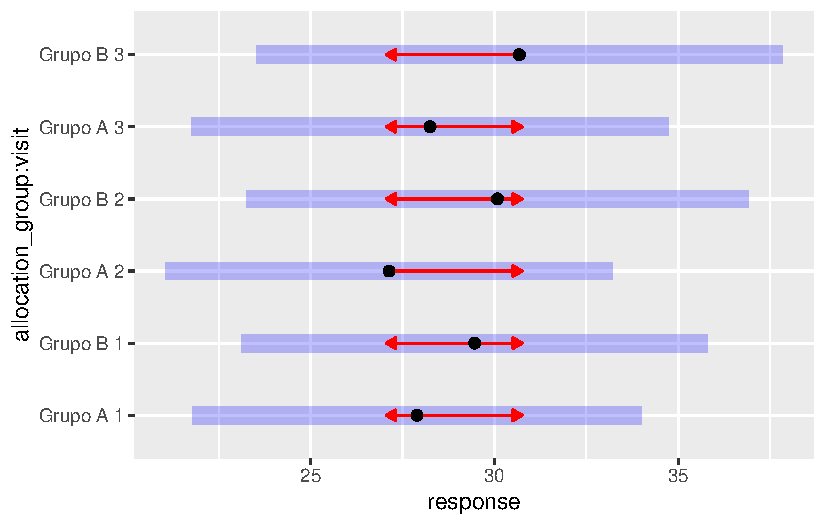
\includegraphics{Outcomes_files/figure-pdf/labs_ggt_raw_emm-1.pdf}

\subparagraph{Análise de
sensibilidade}\label{anuxe1lise-de-sensibilidade-2}

\begin{Shaded}
\begin{Highlighting}[]
\CommentTok{\# Get EMMs for each group at each visit (Sensitivity Analysis)}
\NormalTok{labs\_ggt\_emm }\OtherTok{\textless{}{-}}\NormalTok{ emmeans}\SpecialCharTok{::}\FunctionTok{emmeans}\NormalTok{(}
\NormalTok{    labs\_ggt\_model\_sens, }
    \SpecialCharTok{\textasciitilde{}}\NormalTok{ allocation\_group }\SpecialCharTok{*}\NormalTok{ visit}
\NormalTok{)}

\NormalTok{labs\_ggt\_emm }\OtherTok{\textless{}{-}} \FunctionTok{regrid}\NormalTok{(labs\_ggt\_emm)}

\CommentTok{\# Table of marginal means}
\CommentTok{\# labs\_ggt\_emm}

\CommentTok{\# Pairwise comparisons: Between groups at each visit}
\NormalTok{emmeans}\SpecialCharTok{::}\FunctionTok{contrast}\NormalTok{(labs\_ggt\_emm,}
\AttributeTok{method =} \StringTok{"pairwise"}\NormalTok{, }\AttributeTok{by =} \StringTok{"visit"}\NormalTok{,}
\AttributeTok{adjust =} \StringTok{"bonferroni"}\NormalTok{) }\SpecialCharTok{\%\textgreater{}\%} \FunctionTok{summary}\NormalTok{(}\AttributeTok{infer =} \FunctionTok{c}\NormalTok{(}\ConstantTok{TRUE}\NormalTok{, }\ConstantTok{TRUE}\NormalTok{))}
\end{Highlighting}
\end{Shaded}

\begin{verbatim}
visit = 1:
 contrast          estimate   SE   df lower.CL upper.CL t.ratio p.value
 Grupo A - Grupo B    -3.87 3.49 74.8    -10.8     3.08  -1.110  0.2705

visit = 2:
 contrast          estimate   SE   df lower.CL upper.CL t.ratio p.value
 Grupo A - Grupo B    -5.63 3.73 80.4    -13.0     1.79  -1.510  0.1351

visit = 3:
 contrast          estimate   SE   df lower.CL upper.CL t.ratio p.value
 Grupo A - Grupo B    -4.54 3.92 88.4    -12.3     3.25  -1.158  0.2501

Degrees-of-freedom method: inherited from kenward-roger when re-gridding 
Confidence level used: 0.95 
\end{verbatim}

\begin{Shaded}
\begin{Highlighting}[]
\CommentTok{\# Pairwise comparisons: Changes over time within each group}
\NormalTok{emmeans}\SpecialCharTok{::}\FunctionTok{contrast}\NormalTok{(labs\_ggt\_emm,}
\AttributeTok{method =} \StringTok{"pairwise"}\NormalTok{, }\AttributeTok{by =} \StringTok{"allocation\_group"}\NormalTok{,}
\AttributeTok{adjust =} \StringTok{"bonferroni"}\NormalTok{) }\SpecialCharTok{\%\textgreater{}\%} \FunctionTok{summary}\NormalTok{(}\AttributeTok{infer =} \FunctionTok{c}\NormalTok{(}\ConstantTok{TRUE}\NormalTok{, }\ConstantTok{TRUE}\NormalTok{))}
\end{Highlighting}
\end{Shaded}

\begin{verbatim}
allocation_group = Grupo A:
 contrast        estimate   SE   df lower.CL upper.CL t.ratio p.value
 visit1 - visit2    0.273 1.25 74.8    -2.80     3.34   0.218  1.0000
 visit1 - visit3   -0.986 1.42 74.8    -4.46     2.49  -0.694  1.0000
 visit2 - visit3   -1.259 1.42 80.4    -4.73     2.21  -0.888  1.0000

allocation_group = Grupo B:
 contrast        estimate   SE   df lower.CL upper.CL t.ratio p.value
 visit1 - visit2   -1.479 1.64 74.8    -5.51     2.55  -0.899  1.0000
 visit1 - visit3   -1.649 1.78 74.8    -6.02     2.72  -0.924  1.0000
 visit2 - visit3   -0.170 1.88 90.1    -4.74     4.40  -0.091  1.0000

Degrees-of-freedom method: inherited from kenward-roger when re-gridding 
Confidence level used: 0.95 
Conf-level adjustment: bonferroni method for 3 estimates 
P value adjustment: bonferroni method for 3 tests 
\end{verbatim}

\begin{Shaded}
\begin{Highlighting}[]
\CommentTok{\# Plot of marginal means}
\FunctionTok{plot}\NormalTok{(labs\_ggt\_emm)}
\end{Highlighting}
\end{Shaded}

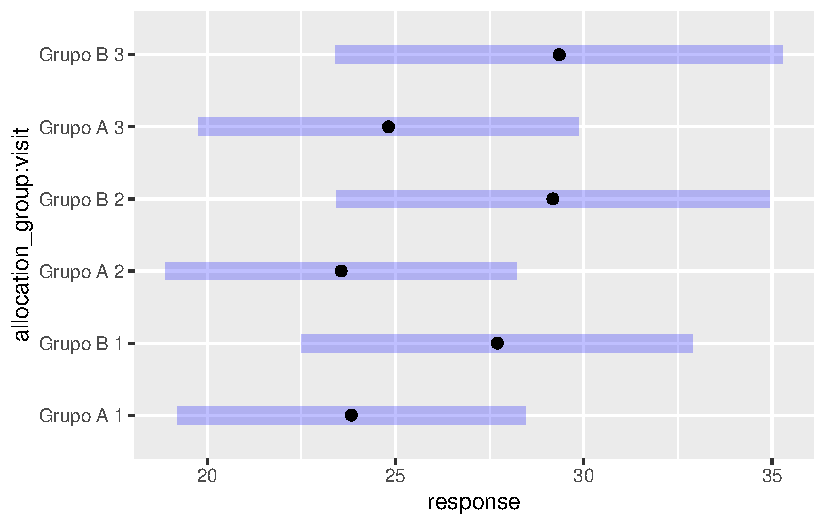
\includegraphics{Outcomes_files/figure-pdf/labs_ggt_sens_emm-1.pdf}

\paragraph{Resultado}\label{resultado-2}

No modelo ajustado para os níveis de Gama Glutamiltransferase (GGT), não
foram observadas diferenças estatisticamente significativas entre os
grupos em nenhum dos três momentos avaliados. Também não foram
identificadas mudanças significativas ao longo do tempo dentro de cada
grupo. A análise de sensibilidade, com exclusão das observações
influentes, não alterou substancialmente os resultados. As estimativas
permaneceram similares, reforçando a ausência de diferenças
significativas entre os grupos ou de variações temporais relevantes. As
estimativas, intervalos de confiança de 95\% e valores de p estão
apresentados na Tabela~\ref{tbl-ggt}.

\begin{longtable}[]{@{}
  >{\raggedright\arraybackslash}p{(\columnwidth - 8\tabcolsep) * \real{0.2000}}
  >{\raggedright\arraybackslash}p{(\columnwidth - 8\tabcolsep) * \real{0.2000}}
  >{\raggedright\arraybackslash}p{(\columnwidth - 8\tabcolsep) * \real{0.2000}}
  >{\raggedright\arraybackslash}p{(\columnwidth - 8\tabcolsep) * \real{0.2000}}
  >{\raggedright\arraybackslash}p{(\columnwidth - 8\tabcolsep) * \real{0.2000}}@{}}
\caption{Diferenças estimadas dos níveis de Gama Glutamiltransferase
(GGT) entre os grupos de alocação (placebo vs Eclipta) e entre visitas
dentro de cada grupo}\label{tbl-ggt}\tabularnewline
\toprule\noalign{}
\begin{minipage}[b]{\linewidth}\raggedright
Grupo de comparação
\end{minipage} & \begin{minipage}[b]{\linewidth}\raggedright
Comparação
\end{minipage} & \begin{minipage}[b]{\linewidth}\raggedright
Estimativa
\end{minipage} & \begin{minipage}[b]{\linewidth}\raggedright
IC 95\%
\end{minipage} & \begin{minipage}[b]{\linewidth}\raggedright
p-valor
\end{minipage} \\
\midrule\noalign{}
\endfirsthead
\toprule\noalign{}
\begin{minipage}[b]{\linewidth}\raggedright
Grupo de comparação
\end{minipage} & \begin{minipage}[b]{\linewidth}\raggedright
Comparação
\end{minipage} & \begin{minipage}[b]{\linewidth}\raggedright
Estimativa
\end{minipage} & \begin{minipage}[b]{\linewidth}\raggedright
IC 95\%
\end{minipage} & \begin{minipage}[b]{\linewidth}\raggedright
p-valor
\end{minipage} \\
\midrule\noalign{}
\endhead
\bottomrule\noalign{}
\endlastfoot
Entre grupos & Visita 1 & -1,57 & {[}-10,4 ; 7,23{]} & 0,724 \\
Entre grupos & Visita 2 & -2,95 & {[}-12,1 ; 6,19{]} & 0,523 \\
Entre grupos & Visita 3 & -2,43 & {[}-12,1 ; 7,24{]} & 0,619 \\
Grupo Placebo & Visita 1 - Visita 2 & 0,76 & {[}-3,48 ; 5,01{]} &
1,000 \\
Grupo Placebo & Visita 1 - Visita 3 & -0,35 & {[}-5,06 ; 4,35{]} &
1,000 \\
Grupo Placebo & Visita 2 - Visita 3 & -1,12 & {[}-5,79 ; 3,56{]} &
1,000 \\
Grupo Eclipta & Visita 1 - Visita 2 & -0,62 & {[}-5,58 ; 4,34{]} &
1,000 \\
Grupo Eclipta & Visita 1 - Visita 3 & -1,22 & {[}-6,69 ; 4,26{]} &
1,000 \\
Grupo Eclipta & Visita 2 - Visita 3 & -0,60 & {[}-6,27 ; 5,08{]} &
1,000 \\
\end{longtable}

\begin{Shaded}
\begin{Highlighting}[]
\FunctionTok{ggplot}\NormalTok{(}
    \AttributeTok{data =}\NormalTok{ data\_model, }
    \FunctionTok{aes}\NormalTok{(}
        \AttributeTok{x =} \FunctionTok{as.factor}\NormalTok{(visit),}
        \AttributeTok{y =}\NormalTok{ labs\_ggt,}
        \AttributeTok{group =}\NormalTok{ record\_id,}
\NormalTok{    )}
\NormalTok{) }\SpecialCharTok{+}
    \FunctionTok{geom\_line}\NormalTok{(}\AttributeTok{alpha =} \FloatTok{0.5}\NormalTok{) }\SpecialCharTok{+}
    \FunctionTok{geom\_point}\NormalTok{(}\AttributeTok{alpha =} \FloatTok{0.7}\NormalTok{) }\SpecialCharTok{+}
    \FunctionTok{geom\_smooth}\NormalTok{(}
        \FunctionTok{aes}\NormalTok{(}\AttributeTok{group =}\NormalTok{ allocation\_group),}
        \AttributeTok{method =} \StringTok{"lm"}\NormalTok{,}
        \AttributeTok{se =} \ConstantTok{TRUE}\NormalTok{,}
        \AttributeTok{linewidth =} \DecValTok{1}
\NormalTok{    ) }\SpecialCharTok{+}
    \FunctionTok{labs}\NormalTok{(}\AttributeTok{title =} \StringTok{"All data"}\NormalTok{) }\SpecialCharTok{+}
    \FunctionTok{facet\_wrap}\NormalTok{(}\SpecialCharTok{\textasciitilde{}}\NormalTok{ allocation\_group) }
\end{Highlighting}
\end{Shaded}

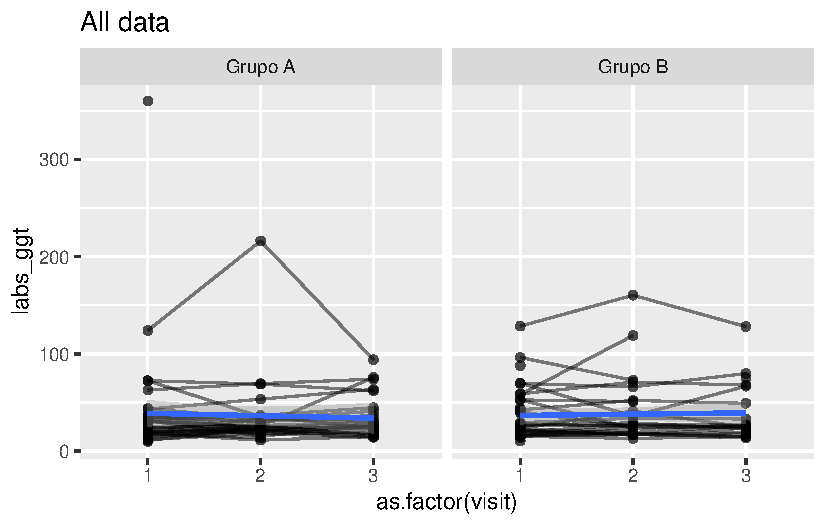
\includegraphics{Outcomes_files/figure-pdf/labs_ggt_6-1.pdf}

\begin{Shaded}
\begin{Highlighting}[]
    \CommentTok{\#coord\_cartesian(ylim = c(10, 150))}

\NormalTok{data\_model }\SpecialCharTok{\%\textgreater{}\%} 
    \FunctionTok{filter}\NormalTok{(}
        \SpecialCharTok{!}\NormalTok{(record\_id }\SpecialCharTok{\%in\%} 
\NormalTok{        labs\_ggt\_model\_check}\SpecialCharTok{$}\NormalTok{influential\_ids)}
\NormalTok{    ) }\SpecialCharTok{\%\textgreater{}\%} 
    \FunctionTok{ggplot}\NormalTok{(}
        \FunctionTok{aes}\NormalTok{(}
            \AttributeTok{x =} \FunctionTok{as.factor}\NormalTok{(visit),}
            \AttributeTok{y =}\NormalTok{ labs\_ggt,}
            \AttributeTok{group =}\NormalTok{ record\_id,}
\NormalTok{        )}
\NormalTok{    ) }\SpecialCharTok{+}
    \FunctionTok{geom\_line}\NormalTok{(}\AttributeTok{alpha =} \FloatTok{0.5}\NormalTok{) }\SpecialCharTok{+}
    \FunctionTok{geom\_point}\NormalTok{(}\AttributeTok{alpha =} \FloatTok{0.7}\NormalTok{) }\SpecialCharTok{+}
    \FunctionTok{geom\_smooth}\NormalTok{(}
        \FunctionTok{aes}\NormalTok{(}\AttributeTok{group =}\NormalTok{ allocation\_group),}
        \AttributeTok{method =} \StringTok{"lm"}\NormalTok{,}
        \AttributeTok{se =} \ConstantTok{TRUE}\NormalTok{,}
        \AttributeTok{linewidth =} \DecValTok{1}
\NormalTok{    ) }\SpecialCharTok{+}
    \FunctionTok{labs}\NormalTok{(}\AttributeTok{title =} \StringTok{"Sensitivity analysis"}\NormalTok{) }\SpecialCharTok{+}
    \FunctionTok{facet\_wrap}\NormalTok{(}\SpecialCharTok{\textasciitilde{}}\NormalTok{ allocation\_group) }
\end{Highlighting}
\end{Shaded}

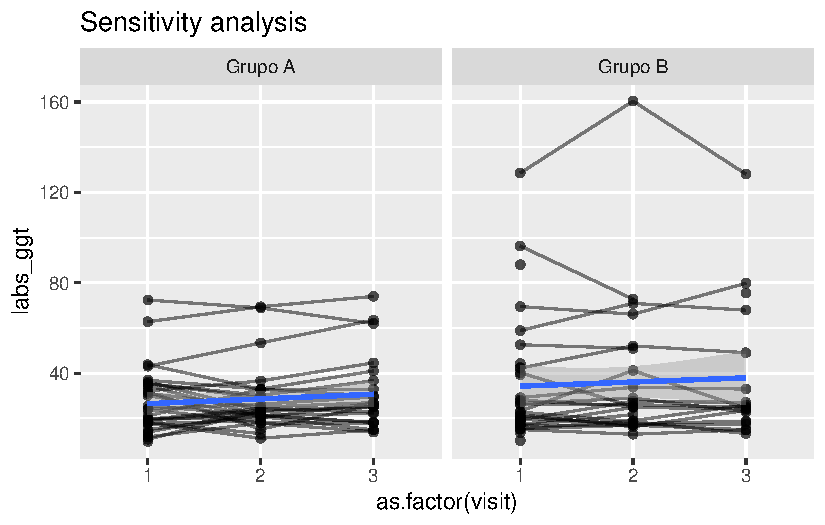
\includegraphics{Outcomes_files/figure-pdf/labs_ggt_6-2.pdf}

\begin{Shaded}
\begin{Highlighting}[]
    \CommentTok{\#coord\_cartesian(ylim = c(10, 150))}
\end{Highlighting}
\end{Shaded}

\subsubsection{Fosfatase Alcalina}\label{fosfatase-alcalina}

Variável: \texttt{labs\_alkp}

\begin{Shaded}
\begin{Highlighting}[]
\CommentTok{\# Plot 1: Raw data}
\NormalTok{labs\_alkp\_hist\_1 }\OtherTok{\textless{}{-}}\NormalTok{ data\_model }\SpecialCharTok{\%\textgreater{}\%} 
    \CommentTok{\#filter(}
    \CommentTok{\#    labs\_alkp \textless{} 300}
    \CommentTok{\#) \%\textgreater{}\% }
    \FunctionTok{ggplot}\NormalTok{(}\FunctionTok{aes}\NormalTok{(}\AttributeTok{x =}\NormalTok{ labs\_alkp)) }\SpecialCharTok{+} 
    \FunctionTok{geom\_histogram}\NormalTok{(}\AttributeTok{bins =} \DecValTok{50}\NormalTok{, }\AttributeTok{fill =} \StringTok{"skyblue"}\NormalTok{, }\AttributeTok{color =} \StringTok{"black"}\NormalTok{)}

\CommentTok{\# Plot 2: Log{-}transformed data}
\NormalTok{labs\_alkp\_hist\_2 }\OtherTok{\textless{}{-}}\NormalTok{ data\_model }\SpecialCharTok{\%\textgreater{}\%} 
    \CommentTok{\#filter(}
    \CommentTok{\#    labs\_alkp \textless{} 300}
    \CommentTok{\#) \%\textgreater{}\%}
    \FunctionTok{ggplot}\NormalTok{(}\FunctionTok{aes}\NormalTok{(}\AttributeTok{x =} \FunctionTok{log1p}\NormalTok{(labs\_alkp))) }\SpecialCharTok{+} 
    \FunctionTok{geom\_histogram}\NormalTok{(}\AttributeTok{bins =} \DecValTok{50}\NormalTok{, }\AttributeTok{fill =} \StringTok{"lightgreen"}\NormalTok{, }\AttributeTok{color =} \StringTok{"black"}\NormalTok{)}

\CommentTok{\# Combine side by side}
\NormalTok{labs\_alkp\_hist\_1 }\SpecialCharTok{+}\NormalTok{ labs\_alkp\_hist\_2 }\CommentTok{\# library(patchwork)}
\end{Highlighting}
\end{Shaded}

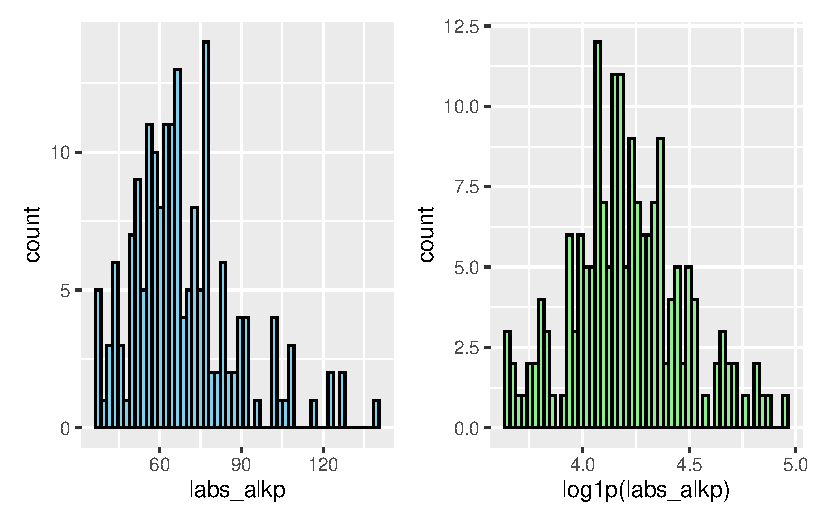
\includegraphics{Outcomes_files/figure-pdf/labs_alkp_1-1.pdf}

\begin{Shaded}
\begin{Highlighting}[]
\CommentTok{\# LMM}
\NormalTok{labs\_alkp\_model }\OtherTok{\textless{}{-}} \FunctionTok{lmer}\NormalTok{(}\FunctionTok{log1p}\NormalTok{(labs\_alkp) }\SpecialCharTok{\textasciitilde{}}\NormalTok{ allocation\_group }\SpecialCharTok{*}\NormalTok{ visit }\SpecialCharTok{+} 
\NormalTok{(}\DecValTok{1} \SpecialCharTok{|}\NormalTok{ record\_id), }\AttributeTok{data =}\NormalTok{ data\_model)}
\FunctionTok{check\_collinearity}\NormalTok{(labs\_alkp\_model)}
\end{Highlighting}
\end{Shaded}

\begin{verbatim}
# Check for Multicollinearity

Low Correlation

                   Term  VIF   VIF 95% CI Increased SE Tolerance Tolerance 95% CI
       allocation_group 1.08 [1.01, 1.62]         1.04      0.93     [0.62, 0.99]
                  visit 3.40 [2.71, 4.36]         1.84      0.29     [0.23, 0.37]
 allocation_group:visit 3.52 [2.80, 4.52]         1.88      0.28     [0.22, 0.36]
\end{verbatim}

\begin{Shaded}
\begin{Highlighting}[]
\CommentTok{\# Sensitivity analysis}
\NormalTok{labs\_alkp\_model\_check }\OtherTok{\textless{}{-}} \FunctionTok{sensitivity\_check\_lmer}\NormalTok{(}
    \AttributeTok{model =}\NormalTok{ labs\_alkp\_model,}
    \AttributeTok{id\_var =} \StringTok{"record\_id"}\NormalTok{,}
    \AttributeTok{top\_n =} \DecValTok{4}\NormalTok{)}

\CommentTok{\# LMM Sensitivity}
\NormalTok{labs\_alkp\_model\_sens }\OtherTok{\textless{}{-}} \FunctionTok{update}\NormalTok{(}\AttributeTok{object =}\NormalTok{ labs\_alkp\_model,}
                              \AttributeTok{subset =} \SpecialCharTok{!}\NormalTok{(record\_id }\SpecialCharTok{\%in\%} 
\NormalTok{        labs\_alkp\_model\_check}\SpecialCharTok{$}\NormalTok{influential\_ids))}
\CommentTok{\# Influential IDS}
\NormalTok{labs\_alkp\_model\_check}\SpecialCharTok{$}\NormalTok{influential\_ids}
\end{Highlighting}
\end{Shaded}

\begin{verbatim}
[1] "56" "75" "53" "3" 
\end{verbatim}

\paragraph{Resumo dos modelos}\label{resumo-dos-modelos-3}

\begin{Shaded}
\begin{Highlighting}[]
\CommentTok{\# Model comparison}
\FunctionTok{summary}\NormalTok{(labs\_alkp\_model)}
\end{Highlighting}
\end{Shaded}

\begin{verbatim}
Linear mixed model fit by REML. t-tests use Satterthwaite's method ['lmerModLmerTest']
Formula: log1p(labs_alkp) ~ allocation_group * visit + (1 | record_id)
   Data: data_model

REML criterion at convergence: -87.9

Scaled residuals: 
     Min       1Q   Median       3Q      Max 
-2.02732 -0.46612  0.01043  0.43200  2.62132 

Random effects:
 Groups    Name        Variance Std.Dev.
 record_id (Intercept) 0.06041  0.2458  
 Residual              0.01021  0.1010  
Number of obs: 178, groups:  record_id, 75

Fixed effects:
                                 Estimate Std. Error         df t value Pr(>|t|)    
(Intercept)                      4.210088   0.043688  84.150015  96.367   <2e-16 ***
allocation_groupGrupo B          0.033160   0.061377  84.150015   0.540   0.5904    
visit2                          -0.046856   0.025510 100.999520  -1.837   0.0692 .  
visit3                          -0.030253   0.027680 101.476417  -1.093   0.2770    
allocation_groupGrupo B:visit2   0.018421   0.037511 101.816342   0.491   0.6244    
allocation_groupGrupo B:visit3   0.004182   0.040741 102.191761   0.103   0.9184    
---
Signif. codes:  0 '***' 0.001 '**' 0.01 '*' 0.05 '.' 0.1 ' ' 1

Correlation of Fixed Effects:
            (Intr) all_GB visit2 visit3 a_GB:2
allctn_grGB -0.712                            
visit2      -0.248  0.176                     
visit3      -0.228  0.162  0.455              
allctn_GB:2  0.168 -0.236 -0.680 -0.310       
allctn_GB:3  0.155 -0.218 -0.309 -0.679  0.436
\end{verbatim}

\begin{Shaded}
\begin{Highlighting}[]
\FunctionTok{summary}\NormalTok{(labs\_alkp\_model\_sens)}
\end{Highlighting}
\end{Shaded}

\begin{verbatim}
Linear mixed model fit by REML. t-tests use Satterthwaite's method ['lmerModLmerTest']
Formula: log1p(labs_alkp) ~ allocation_group * visit + (1 | record_id)
   Data: data_model
 Subset: !(record_id %in% labs_alkp_model_check$influential_ids)

REML criterion at convergence: -118.6

Scaled residuals: 
     Min       1Q   Median       3Q      Max 
-1.95508 -0.49130  0.04228  0.50567  1.80928 

Random effects:
 Groups    Name        Variance Std.Dev.
 record_id (Intercept) 0.06287  0.25073 
 Residual              0.00669  0.08179 
Number of obs: 167, groups:  record_id, 71

Fixed effects:
                                Estimate Std. Error        df t value Pr(>|t|)    
(Intercept)                     4.198426   0.044579 75.550975  94.179   <2e-16 ***
allocation_groupGrupo B         0.071738   0.062605 75.550975   1.146    0.255    
visit2                         -0.021391   0.021391 93.237481  -1.000    0.320    
visit3                         -0.002867   0.023373 93.517548  -0.123    0.903    
allocation_groupGrupo B:visit2 -0.020052   0.031577 93.770609  -0.635    0.527    
allocation_groupGrupo B:visit3 -0.052680   0.034183 93.954152  -1.541    0.127    
---
Signif. codes:  0 '***' 0.001 '**' 0.01 '*' 0.05 '.' 0.1 ' ' 1

Correlation of Fixed Effects:
            (Intr) all_GB visit2 visit3 a_GB:2
allctn_grGB -0.712                            
visit2      -0.200  0.143                     
visit3      -0.183  0.131  0.454              
allctn_GB:2  0.136 -0.191 -0.677 -0.307       
allctn_GB:3  0.125 -0.176 -0.310 -0.684  0.438
\end{verbatim}

\begin{Shaded}
\begin{Highlighting}[]
\NormalTok{labs\_alkp\_model\_check}\SpecialCharTok{$}\NormalTok{comparison\_table}
\end{Highlighting}
\end{Shaded}

\begin{verbatim}
# A tibble: 16 x 6
   Model       term                           estimate std.error statistic   p.value
   <chr>       <chr>                             <dbl>     <dbl>     <dbl>     <dbl>
 1 Original    (Intercept)                     4.21       0.0437    96.4    6.67e-88
 2 Sensitivity (Intercept)                     4.20       0.0446    94.2    4.38e-80
 3 Original    allocation_groupGrupo B         0.0332     0.0614     0.540  5.90e- 1
 4 Sensitivity allocation_groupGrupo B         0.0717     0.0626     1.15   2.55e- 1
 5 Original    allocation_groupGrupo B:visit2  0.0184     0.0375     0.491  6.24e- 1
 6 Sensitivity allocation_groupGrupo B:visit2 -0.0201     0.0316    -0.635  5.27e- 1
 7 Original    allocation_groupGrupo B:visit3  0.00418    0.0407     0.103  9.18e- 1
 8 Sensitivity allocation_groupGrupo B:visit3 -0.0527     0.0342    -1.54   1.27e- 1
 9 Original    sd__(Intercept)                 0.246     NA         NA     NA       
10 Sensitivity sd__(Intercept)                 0.251     NA         NA     NA       
11 Original    sd__Observation                 0.101     NA         NA     NA       
12 Sensitivity sd__Observation                 0.0818    NA         NA     NA       
13 Original    visit2                         -0.0469     0.0255    -1.84   6.92e- 2
14 Sensitivity visit2                         -0.0214     0.0214    -1.00   3.20e- 1
15 Original    visit3                         -0.0303     0.0277    -1.09   2.77e- 1
16 Sensitivity visit3                         -0.00287    0.0234    -0.123  9.03e- 1
\end{verbatim}

\begin{Shaded}
\begin{Highlighting}[]
\NormalTok{performance}\SpecialCharTok{::}\FunctionTok{compare\_performance}\NormalTok{(}
\NormalTok{    labs\_alkp\_model, }
\NormalTok{    labs\_alkp\_model\_sens) }
\end{Highlighting}
\end{Shaded}

\begin{verbatim}
# Comparison of Model Performance Indices

Name                 |           Model |  AIC (weights) | AICc (weights) |  BIC (weights) | R2 (cond.) | R2 (marg.) |   ICC |  RMSE | Sigma
-------------------------------------------------------------------------------------------------------------------------------------------
labs_alkp_model      | lmerModLmerTest | 1394.9 (<.001) | 1395.7 (<.001) | 1420.3 (<.001) |      0.857 |      0.010 | 0.855 | 0.077 | 0.101
labs_alkp_model_sens | lmerModLmerTest | 1274.2 (>.999) | 1275.1 (>.999) | 1299.1 (>.999) |      0.905 |      0.015 | 0.904 | 0.062 | 0.082
\end{verbatim}

\begin{Shaded}
\begin{Highlighting}[]
\NormalTok{performance}\SpecialCharTok{::}\FunctionTok{check\_model}\NormalTok{(labs\_alkp\_model)}
\end{Highlighting}
\end{Shaded}

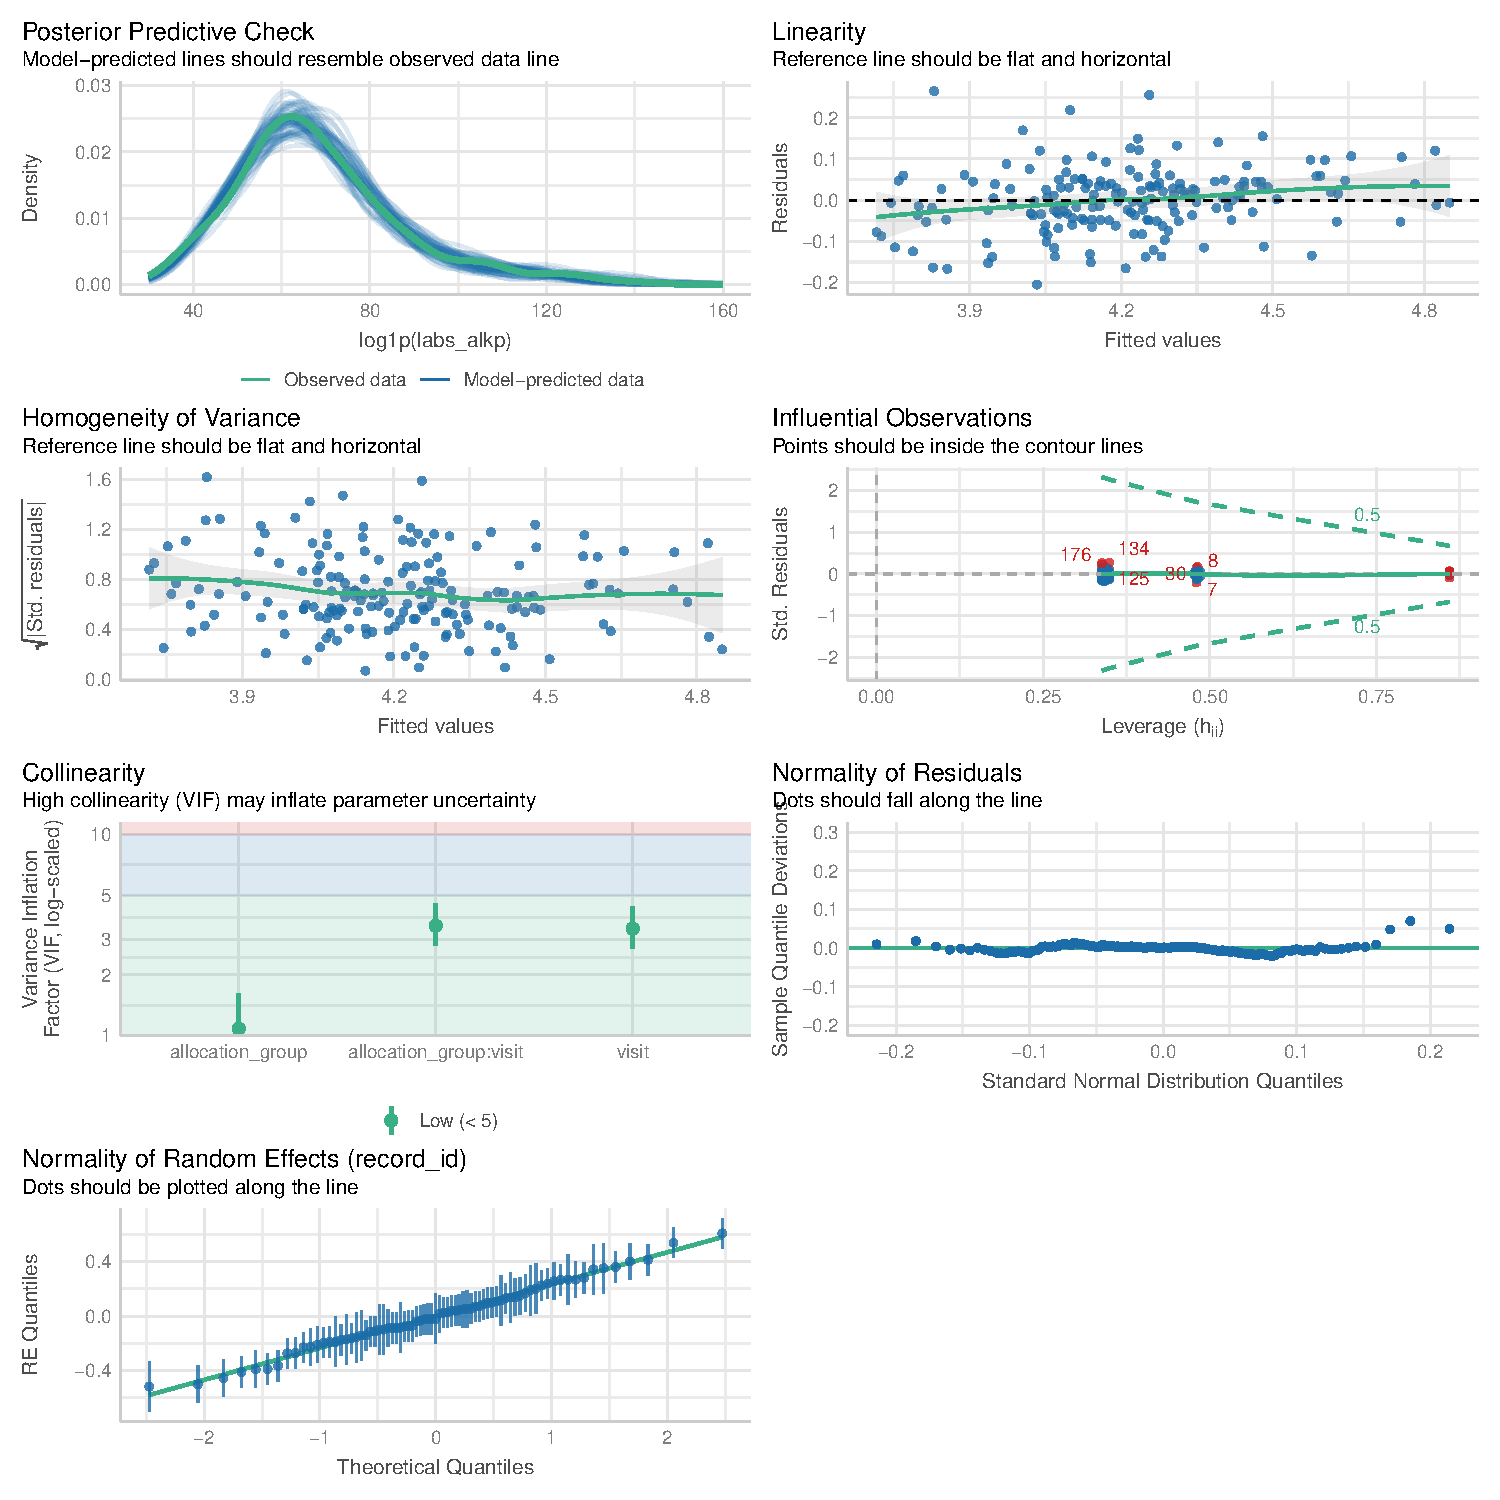
\includegraphics{Outcomes_files/figure-pdf/labs_alkp_4-1.pdf}

\begin{Shaded}
\begin{Highlighting}[]
\NormalTok{performance}\SpecialCharTok{::}\FunctionTok{check\_model}\NormalTok{(labs\_alkp\_model\_sens)}
\end{Highlighting}
\end{Shaded}

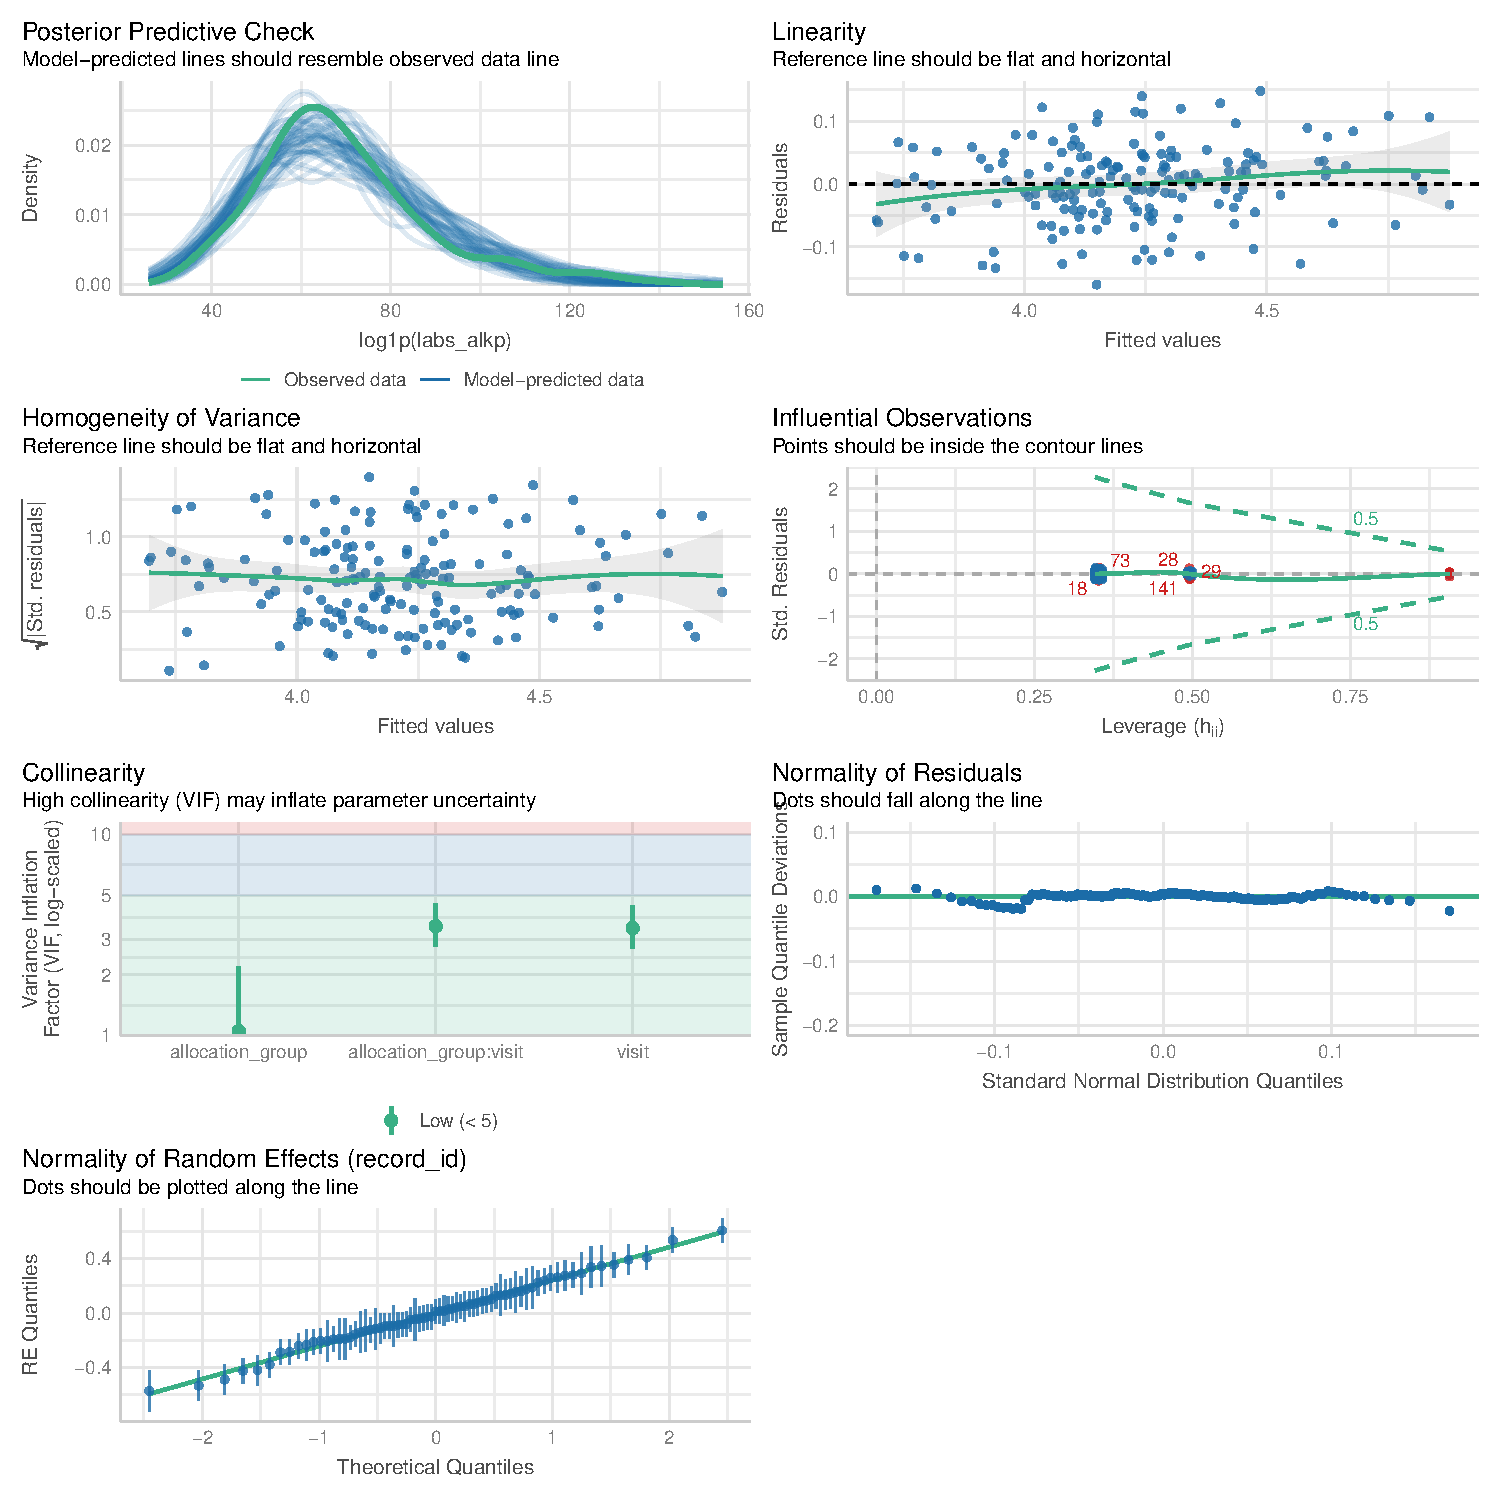
\includegraphics{Outcomes_files/figure-pdf/labs_alkp_4-2.pdf}

\paragraph{Médias Marginais
Estimadas}\label{muxe9dias-marginais-estimadas-3}

\subparagraph{Todos os dados}\label{todos-os-dados-3}

\begin{Shaded}
\begin{Highlighting}[]
\CommentTok{\# Get EMMs for each group at each visit }
\NormalTok{labs\_alkp\_raw\_emm }\OtherTok{\textless{}{-}}\NormalTok{ emmeans}\SpecialCharTok{::}\FunctionTok{emmeans}\NormalTok{(}
\NormalTok{    labs\_alkp\_model, }
    \SpecialCharTok{\textasciitilde{}}\NormalTok{ allocation\_group }\SpecialCharTok{*}\NormalTok{ visit}
\NormalTok{)}

\NormalTok{labs\_alkp\_raw\_emm }\OtherTok{\textless{}{-}} \FunctionTok{regrid}\NormalTok{(labs\_alkp\_raw\_emm)}

\CommentTok{\# Table of marginal means}
\CommentTok{\# labs\_alkp\_raw\_emm}

\CommentTok{\# Pairwise comparisons: Between groups at each visit}
\NormalTok{emmeans}\SpecialCharTok{::}\FunctionTok{contrast}\NormalTok{(labs\_alkp\_raw\_emm,}
\AttributeTok{method =} \StringTok{"pairwise"}\NormalTok{, }\AttributeTok{by =} \StringTok{"visit"}\NormalTok{,}
\AttributeTok{adjust =} \StringTok{"bonferroni"}\NormalTok{) }\SpecialCharTok{\%\textgreater{}\%} \FunctionTok{summary}\NormalTok{(}\AttributeTok{infer =} \FunctionTok{c}\NormalTok{(}\ConstantTok{TRUE}\NormalTok{, }\ConstantTok{TRUE}\NormalTok{))}
\end{Highlighting}
\end{Shaded}

\begin{verbatim}
visit = 1:
 contrast          estimate   SE    df lower.CL upper.CL t.ratio p.value
 Grupo A - Grupo B    -2.27 4.20  84.5    -10.6     6.09  -0.540  0.5904

visit = 2:
 contrast          estimate   SE    df lower.CL upper.CL t.ratio p.value
 Grupo A - Grupo B    -3.40 4.22  92.0    -11.8     4.98  -0.806  0.4223

visit = 3:
 contrast          estimate   SE    df lower.CL upper.CL t.ratio p.value
 Grupo A - Grupo B    -2.49 4.39 101.0    -11.2     6.22  -0.566  0.5724

Degrees-of-freedom method: inherited from kenward-roger when re-gridding 
Confidence level used: 0.95 
\end{verbatim}

\begin{Shaded}
\begin{Highlighting}[]
\CommentTok{\# Pairwise comparisons: Changes over time within each group}
\NormalTok{emmeans}\SpecialCharTok{::}\FunctionTok{contrast}\NormalTok{(labs\_alkp\_raw\_emm,}
\AttributeTok{method =} \StringTok{"pairwise"}\NormalTok{, }\AttributeTok{by =} \StringTok{"allocation\_group"}\NormalTok{,}
\AttributeTok{adjust =} \StringTok{"bonferroni"}\NormalTok{) }\SpecialCharTok{\%\textgreater{}\%} \FunctionTok{summary}\NormalTok{(}\AttributeTok{infer =} \FunctionTok{c}\NormalTok{(}\ConstantTok{TRUE}\NormalTok{, }\ConstantTok{TRUE}\NormalTok{))}
\end{Highlighting}
\end{Shaded}

\begin{verbatim}
allocation_group = Grupo A:
 contrast        estimate   SE    df lower.CL upper.CL t.ratio p.value
 visit1 - visit2     3.08 1.68  84.5    -1.02     7.18   1.837  0.2094
 visit1 - visit3     2.01 1.83  84.5    -2.47     6.48   1.096  0.8290
 visit2 - visit3    -1.08 1.81  92.0    -5.48     3.33  -0.596  1.0000

allocation_group = Grupo B:
 contrast        estimate   SE    df lower.CL upper.CL t.ratio p.value
 visit1 - visit2     1.95 1.88  84.5    -2.65     6.55   1.036  0.9090
 visit1 - visit3     1.79 2.05  84.5    -3.21     6.79   0.875  1.0000
 visit2 - visit3    -0.16 2.10 101.5    -5.28     4.96  -0.076  1.0000

Degrees-of-freedom method: inherited from kenward-roger when re-gridding 
Confidence level used: 0.95 
Conf-level adjustment: bonferroni method for 3 estimates 
P value adjustment: bonferroni method for 3 tests 
\end{verbatim}

\begin{Shaded}
\begin{Highlighting}[]
\CommentTok{\# Plot of marginal means}
\FunctionTok{plot}\NormalTok{(labs\_alkp\_raw\_emm)}
\end{Highlighting}
\end{Shaded}

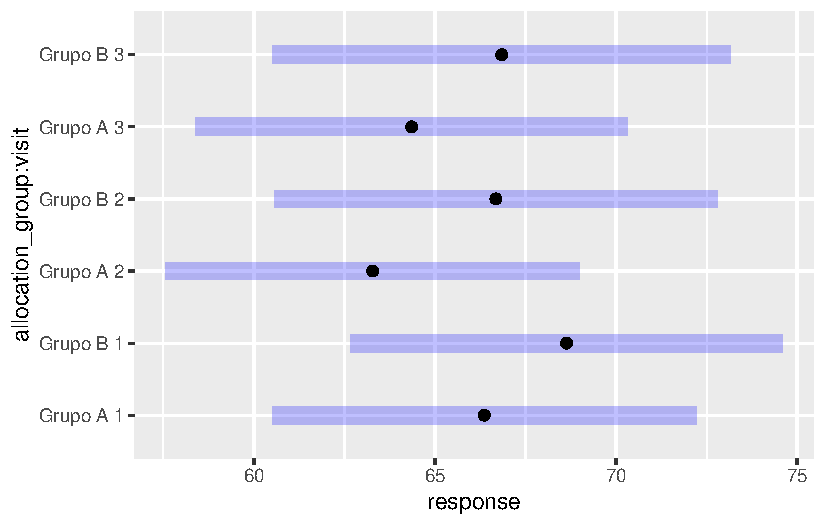
\includegraphics{Outcomes_files/figure-pdf/labs_alkp_raw_emm-1.pdf}

\subparagraph{Análise de
sensibilidade}\label{anuxe1lise-de-sensibilidade-3}

\begin{Shaded}
\begin{Highlighting}[]
\CommentTok{\# Get EMMs for each group at each visit (Sensitivity Analysis)}
\NormalTok{labs\_alkp\_emm }\OtherTok{\textless{}{-}}\NormalTok{ emmeans}\SpecialCharTok{::}\FunctionTok{emmeans}\NormalTok{(}
\NormalTok{    labs\_alkp\_model\_sens, }
    \SpecialCharTok{\textasciitilde{}}\NormalTok{ allocation\_group }\SpecialCharTok{*}\NormalTok{ visit}
\NormalTok{)}

\CommentTok{\# Table of marginal means}
\CommentTok{\# labs\_alkp\_emm}

\CommentTok{\# Pairwise comparisons: Between groups at each visit}
\NormalTok{emmeans}\SpecialCharTok{::}\FunctionTok{contrast}\NormalTok{(labs\_alkp\_emm,}
\AttributeTok{method =} \StringTok{"pairwise"}\NormalTok{, }\AttributeTok{by =} \StringTok{"visit"}\NormalTok{,}
\AttributeTok{adjust =} \StringTok{"bonferroni"}\NormalTok{) }\SpecialCharTok{\%\textgreater{}\%} \FunctionTok{summary}\NormalTok{(}\AttributeTok{infer =} \FunctionTok{c}\NormalTok{(}\ConstantTok{TRUE}\NormalTok{, }\ConstantTok{TRUE}\NormalTok{))}
\end{Highlighting}
\end{Shaded}

\begin{verbatim}
visit = 1:
 contrast          estimate     SE   df lower.CL upper.CL t.ratio p.value
 Grupo A - Grupo B  -0.0717 0.0626 75.8   -0.196   0.0530  -1.146  0.2554

visit = 2:
 contrast          estimate     SE   df lower.CL upper.CL t.ratio p.value
 Grupo A - Grupo B  -0.0517 0.0645 84.4   -0.180   0.0766  -0.801  0.4254

visit = 3:
 contrast          estimate     SE   df lower.CL upper.CL t.ratio p.value
 Grupo A - Grupo B  -0.0191 0.0658 90.6   -0.150   0.1117  -0.289  0.7729

Note: contrasts are still on the log1p scale. Consider using
      regrid() if you want contrasts of back-transformed estimates. 
Degrees-of-freedom method: kenward-roger 
Confidence level used: 0.95 
\end{verbatim}

\begin{Shaded}
\begin{Highlighting}[]
\CommentTok{\# Pairwise comparisons: Changes over time within each group}
\NormalTok{emmeans}\SpecialCharTok{::}\FunctionTok{contrast}\NormalTok{(labs\_alkp\_emm,}
\AttributeTok{method =} \StringTok{"pairwise"}\NormalTok{, }\AttributeTok{by =} \StringTok{"allocation\_group"}\NormalTok{,}
\AttributeTok{adjust =} \StringTok{"bonferroni"}\NormalTok{) }\SpecialCharTok{\%\textgreater{}\%} \FunctionTok{summary}\NormalTok{(}\AttributeTok{infer =} \FunctionTok{c}\NormalTok{(}\ConstantTok{TRUE}\NormalTok{, }\ConstantTok{TRUE}\NormalTok{))}
\end{Highlighting}
\end{Shaded}

\begin{verbatim}
allocation_group = Grupo A:
 contrast        estimate     SE   df lower.CL upper.CL t.ratio p.value
 visit1 - visit2  0.02139 0.0214 93.5 -0.03077   0.0736   1.000  0.9602
 visit1 - visit3  0.00287 0.0234 93.8 -0.05413   0.0599   0.123  1.0000
 visit2 - visit3 -0.01852 0.0235 92.6 -0.07572   0.0387  -0.790  1.0000

allocation_group = Grupo B:
 contrast        estimate     SE   df lower.CL upper.CL t.ratio p.value
 visit1 - visit2  0.04144 0.0232 94.5 -0.01521   0.0981   1.783  0.2333
 visit1 - visit3  0.05555 0.0250 94.6 -0.00529   0.1164   2.225  0.0853
 visit2 - visit3  0.01410 0.0259 92.9 -0.04902   0.0772   0.545  1.0000

Note: contrasts are still on the log1p scale. Consider using
      regrid() if you want contrasts of back-transformed estimates. 
Degrees-of-freedom method: kenward-roger 
Confidence level used: 0.95 
Conf-level adjustment: bonferroni method for 3 estimates 
P value adjustment: bonferroni method for 3 tests 
\end{verbatim}

\begin{Shaded}
\begin{Highlighting}[]
\CommentTok{\# Plot of marginal means}
\FunctionTok{plot}\NormalTok{(labs\_alkp\_emm)}
\end{Highlighting}
\end{Shaded}

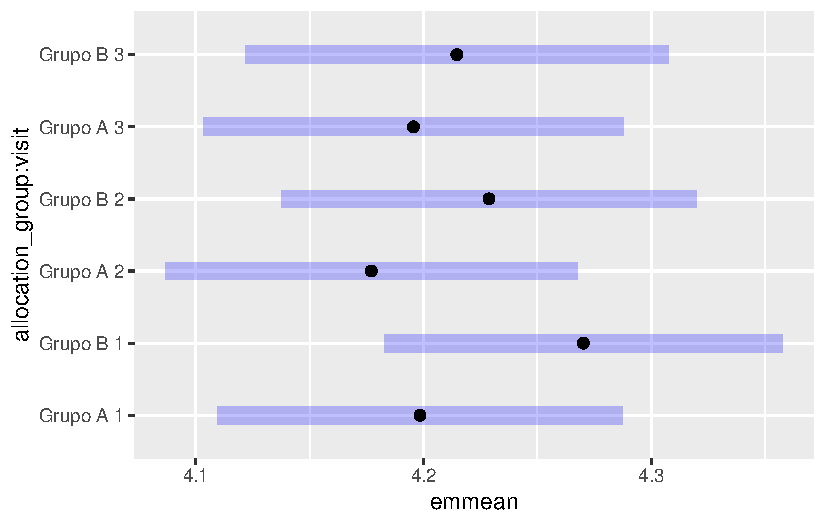
\includegraphics{Outcomes_files/figure-pdf/labs_alkp_sens_emm-1.pdf}

\paragraph{Resultado}\label{resultado-3}

No modelo ajustado para os níveis de Fosfatase Alcalina (ALP), não foram
observadas diferenças estatisticamente significativas entre os grupos em
nenhum dos três momentos avaliados. Da mesma forma, as comparações
intragrupo ao longo do tempo não indicaram variações significativas. A
análise de sensibilidade, realizada com exclusão das observações
influentes, manteve os resultados essencialmente inalterados, com
estimativas semelhantes e ausência de significância estatística nas
comparações entre grupos e entre visitas. As estimativas, intervalos de
confiança de 95\% e valores de p estão apresentados na
Tabela~\ref{tbl-alkp}.

\begin{longtable}[]{@{}
  >{\raggedright\arraybackslash}p{(\columnwidth - 8\tabcolsep) * \real{0.2000}}
  >{\raggedright\arraybackslash}p{(\columnwidth - 8\tabcolsep) * \real{0.2000}}
  >{\raggedright\arraybackslash}p{(\columnwidth - 8\tabcolsep) * \real{0.2000}}
  >{\raggedright\arraybackslash}p{(\columnwidth - 8\tabcolsep) * \real{0.2000}}
  >{\raggedright\arraybackslash}p{(\columnwidth - 8\tabcolsep) * \real{0.2000}}@{}}
\caption{Diferenças estimadas dos níveis de Fosfatase Alcalina (ALP)
entre os grupos de alocação (placebo vs Eclipta) e entre visitas dentro
de cada grupo}\label{tbl-alkp}\tabularnewline
\toprule\noalign{}
\begin{minipage}[b]{\linewidth}\raggedright
Grupo de comparação
\end{minipage} & \begin{minipage}[b]{\linewidth}\raggedright
Comparação
\end{minipage} & \begin{minipage}[b]{\linewidth}\raggedright
Estimativa
\end{minipage} & \begin{minipage}[b]{\linewidth}\raggedright
IC 95\%
\end{minipage} & \begin{minipage}[b]{\linewidth}\raggedright
p-valor
\end{minipage} \\
\midrule\noalign{}
\endfirsthead
\toprule\noalign{}
\begin{minipage}[b]{\linewidth}\raggedright
Grupo de comparação
\end{minipage} & \begin{minipage}[b]{\linewidth}\raggedright
Comparação
\end{minipage} & \begin{minipage}[b]{\linewidth}\raggedright
Estimativa
\end{minipage} & \begin{minipage}[b]{\linewidth}\raggedright
IC 95\%
\end{minipage} & \begin{minipage}[b]{\linewidth}\raggedright
p-valor
\end{minipage} \\
\midrule\noalign{}
\endhead
\bottomrule\noalign{}
\endlastfoot
Entre grupos & Visita 1 & -2,27 & {[}-10,6 ; 6,09{]} & 0,590 \\
Entre grupos & Visita 2 & -3,40 & {[}-11,8 ; 4,98{]} & 0,422 \\
Entre grupos & Visita 3 & -2,49 & {[}-11,2 ; 6,22{]} & 0,572 \\
Grupo Placebo & Visita 1 - Visita 2 & 3,08 & {[}-1,02 ; 7,18{]} &
0,209 \\
Grupo Placebo & Visita 1 - Visita 3 & 2,01 & {[}-2,47 ; 6,48{]} &
0,829 \\
Grupo Placebo & Visita 2 - Visita 3 & -1,08 & {[}-5,48 ; 3,33{]} &
1,000 \\
Grupo Eclipta & Visita 1 - Visita 2 & 1,95 & {[}-2,65 ; 6,55{]} &
0,909 \\
Grupo Eclipta & Visita 1 - Visita 3 & 1,79 & {[}-3,21 ; 6,79{]} &
1,000 \\
Grupo Eclipta & Visita 2 - Visita 3 & -0,16 & {[}-5,28 ; 4,96{]} &
1,000 \\
\end{longtable}

\begin{Shaded}
\begin{Highlighting}[]
\FunctionTok{ggplot}\NormalTok{(}
    \AttributeTok{data =}\NormalTok{ data\_model, }
    \FunctionTok{aes}\NormalTok{(}
        \AttributeTok{x =} \FunctionTok{as.factor}\NormalTok{(visit),}
        \AttributeTok{y =}\NormalTok{ labs\_alkp,}
        \AttributeTok{group =}\NormalTok{ record\_id,}
\NormalTok{    )}
\NormalTok{) }\SpecialCharTok{+}
    \FunctionTok{geom\_line}\NormalTok{(}\AttributeTok{alpha =} \FloatTok{0.5}\NormalTok{) }\SpecialCharTok{+}
    \FunctionTok{geom\_point}\NormalTok{(}\AttributeTok{alpha =} \FloatTok{0.7}\NormalTok{) }\SpecialCharTok{+}
    \FunctionTok{geom\_smooth}\NormalTok{(}
        \FunctionTok{aes}\NormalTok{(}\AttributeTok{group =}\NormalTok{ allocation\_group),}
        \AttributeTok{method =} \StringTok{"lm"}\NormalTok{,}
        \AttributeTok{se =} \ConstantTok{TRUE}\NormalTok{,}
        \AttributeTok{linewidth =} \DecValTok{1}
\NormalTok{    ) }\SpecialCharTok{+}
    \FunctionTok{labs}\NormalTok{(}\AttributeTok{title =} \StringTok{"All data"}\NormalTok{) }\SpecialCharTok{+}
    \FunctionTok{facet\_wrap}\NormalTok{(}\SpecialCharTok{\textasciitilde{}}\NormalTok{ allocation\_group) }
\end{Highlighting}
\end{Shaded}

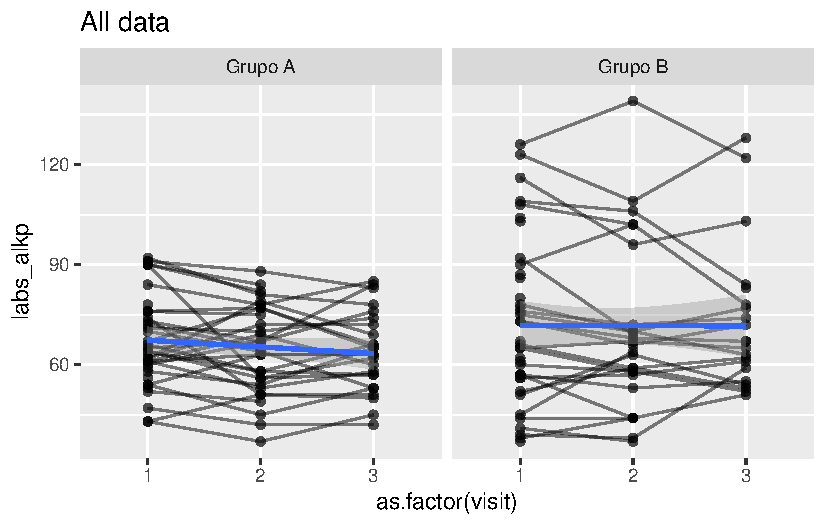
\includegraphics{Outcomes_files/figure-pdf/labs_alkp_6-1.pdf}

\begin{Shaded}
\begin{Highlighting}[]
    \CommentTok{\#coord\_cartesian(ylim = c(10, 150))}

\NormalTok{data\_model }\SpecialCharTok{\%\textgreater{}\%} 
    \FunctionTok{filter}\NormalTok{(}
        \SpecialCharTok{!}\NormalTok{(record\_id }\SpecialCharTok{\%in\%} 
\NormalTok{        labs\_alkp\_model\_check}\SpecialCharTok{$}\NormalTok{influential\_ids)}
\NormalTok{    ) }\SpecialCharTok{\%\textgreater{}\%} 
    \FunctionTok{ggplot}\NormalTok{(}
        \FunctionTok{aes}\NormalTok{(}
            \AttributeTok{x =} \FunctionTok{as.factor}\NormalTok{(visit),}
            \AttributeTok{y =}\NormalTok{ labs\_alkp,}
            \AttributeTok{group =}\NormalTok{ record\_id,}
\NormalTok{        )}
\NormalTok{    ) }\SpecialCharTok{+}
    \FunctionTok{geom\_line}\NormalTok{(}\AttributeTok{alpha =} \FloatTok{0.5}\NormalTok{) }\SpecialCharTok{+}
    \FunctionTok{geom\_point}\NormalTok{(}\AttributeTok{alpha =} \FloatTok{0.7}\NormalTok{) }\SpecialCharTok{+}
    \FunctionTok{geom\_smooth}\NormalTok{(}
        \FunctionTok{aes}\NormalTok{(}\AttributeTok{group =}\NormalTok{ allocation\_group),}
        \AttributeTok{method =} \StringTok{"lm"}\NormalTok{,}
        \AttributeTok{se =} \ConstantTok{TRUE}\NormalTok{,}
        \AttributeTok{linewidth =} \DecValTok{1}
\NormalTok{    ) }\SpecialCharTok{+}
    \FunctionTok{labs}\NormalTok{(}\AttributeTok{title =} \StringTok{"Sensitivity analysis"}\NormalTok{) }\SpecialCharTok{+}
    \FunctionTok{facet\_wrap}\NormalTok{(}\SpecialCharTok{\textasciitilde{}}\NormalTok{ allocation\_group) }
\end{Highlighting}
\end{Shaded}

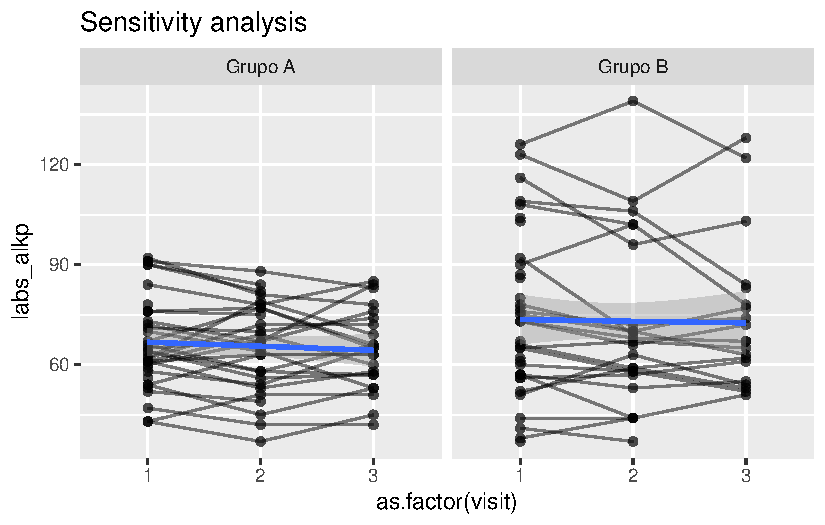
\includegraphics{Outcomes_files/figure-pdf/labs_alkp_6-2.pdf}

\begin{Shaded}
\begin{Highlighting}[]
    \CommentTok{\#coord\_cartesian(ylim = c(10, 150))}
\end{Highlighting}
\end{Shaded}

\subsubsection{Colesterol Total}\label{colesterol-total}

Variável: \texttt{labs\_cholesterol}

\begin{Shaded}
\begin{Highlighting}[]
\CommentTok{\# Plot 1: Raw data}
\NormalTok{labs\_cholesterol\_hist\_1 }\OtherTok{\textless{}{-}}\NormalTok{ data\_model }\SpecialCharTok{\%\textgreater{}\%} 
    \CommentTok{\#filter(}
    \CommentTok{\#    labs\_cholesterol \textless{} 300}
    \CommentTok{\#) \%\textgreater{}\% }
    \FunctionTok{ggplot}\NormalTok{(}\FunctionTok{aes}\NormalTok{(}\AttributeTok{x =}\NormalTok{ labs\_cholesterol)) }\SpecialCharTok{+} 
    \FunctionTok{geom\_histogram}\NormalTok{(}\AttributeTok{bins =} \DecValTok{50}\NormalTok{, }\AttributeTok{fill =} \StringTok{"skyblue"}\NormalTok{, }\AttributeTok{color =} \StringTok{"black"}\NormalTok{)}

\CommentTok{\# Plot 2: Log{-}transformed data}
\NormalTok{labs\_cholesterol\_hist\_2 }\OtherTok{\textless{}{-}}\NormalTok{ data\_model }\SpecialCharTok{\%\textgreater{}\%} 
    \CommentTok{\#filter(}
    \CommentTok{\#    labs\_cholesterol \textless{} 300}
    \CommentTok{\#) \%\textgreater{}\%}
    \FunctionTok{ggplot}\NormalTok{(}\FunctionTok{aes}\NormalTok{(}\AttributeTok{x =} \FunctionTok{log1p}\NormalTok{(labs\_cholesterol))) }\SpecialCharTok{+} 
    \FunctionTok{geom\_histogram}\NormalTok{(}\AttributeTok{bins =} \DecValTok{50}\NormalTok{, }\AttributeTok{fill =} \StringTok{"lightgreen"}\NormalTok{, }\AttributeTok{color =} \StringTok{"black"}\NormalTok{)}

\CommentTok{\# Combine side by side}
\NormalTok{labs\_cholesterol\_hist\_1 }\SpecialCharTok{+}\NormalTok{ labs\_cholesterol\_hist\_2 }\CommentTok{\# library(patchwork)}
\end{Highlighting}
\end{Shaded}

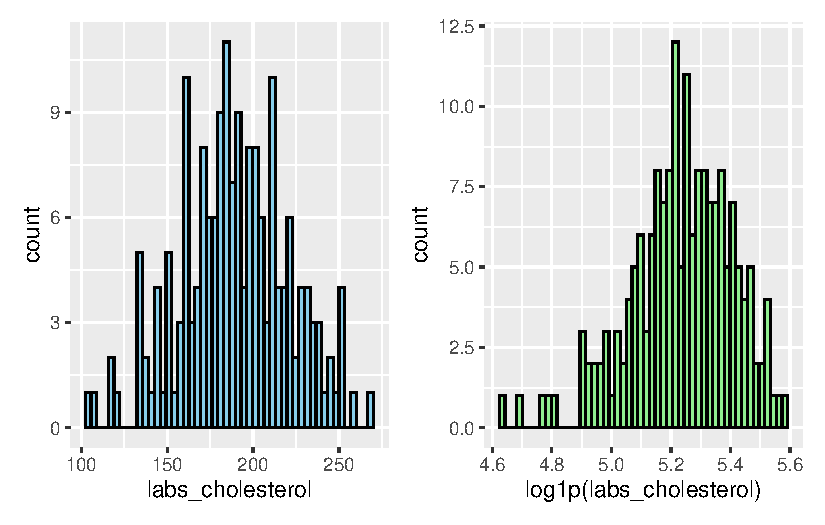
\includegraphics{Outcomes_files/figure-pdf/labs_cholesterol_1-1.pdf}

\begin{Shaded}
\begin{Highlighting}[]
\CommentTok{\# LMM}
\NormalTok{labs\_cholesterol\_model }\OtherTok{\textless{}{-}} \FunctionTok{lmer}\NormalTok{(labs\_cholesterol }\SpecialCharTok{\textasciitilde{}}\NormalTok{ allocation\_group }\SpecialCharTok{*}\NormalTok{ visit }\SpecialCharTok{+} 
\NormalTok{(}\DecValTok{1} \SpecialCharTok{|}\NormalTok{ record\_id), }\AttributeTok{data =}\NormalTok{ data\_model)}
\FunctionTok{check\_collinearity}\NormalTok{(labs\_cholesterol\_model)}
\end{Highlighting}
\end{Shaded}

\begin{verbatim}
# Check for Multicollinearity

Low Correlation

                   Term  VIF   VIF 95% CI Increased SE Tolerance Tolerance 95% CI
       allocation_group 1.15 [1.05, 1.50]         1.07      0.87     [0.67, 0.96]
                  visit 3.49 [2.78, 4.48]         1.87      0.29     [0.22, 0.36]
 allocation_group:visit 3.73 [2.96, 4.80]         1.93      0.27     [0.21, 0.34]
\end{verbatim}

\begin{Shaded}
\begin{Highlighting}[]
\CommentTok{\# Sensitivity analysis}
\NormalTok{labs\_cholesterol\_model\_check }\OtherTok{\textless{}{-}} \FunctionTok{sensitivity\_check\_lmer}\NormalTok{(}
    \AttributeTok{model =}\NormalTok{ labs\_cholesterol\_model,}
    \AttributeTok{id\_var =} \StringTok{"record\_id"}\NormalTok{,}
    \AttributeTok{top\_n =} \DecValTok{5}\NormalTok{)}

\CommentTok{\# LMM Sensitivity}
\NormalTok{labs\_cholesterol\_model\_sens }\OtherTok{\textless{}{-}} \FunctionTok{update}\NormalTok{(}\AttributeTok{object =}\NormalTok{ labs\_cholesterol\_model,}
                              \AttributeTok{subset =} \SpecialCharTok{!}\NormalTok{(record\_id }\SpecialCharTok{\%in\%} 
\NormalTok{        labs\_cholesterol\_model\_check}\SpecialCharTok{$}\NormalTok{influential\_ids))}
\CommentTok{\# Influential IDS}
\NormalTok{labs\_cholesterol\_model\_check}\SpecialCharTok{$}\NormalTok{influential\_ids}
\end{Highlighting}
\end{Shaded}

\begin{verbatim}
[1] "17" "37" "56" "61" "13"
\end{verbatim}

\paragraph{Resumo dos modelos}\label{resumo-dos-modelos-4}

\begin{Shaded}
\begin{Highlighting}[]
\CommentTok{\# Model comparison}
\FunctionTok{summary}\NormalTok{(labs\_cholesterol\_model)}
\end{Highlighting}
\end{Shaded}

\begin{verbatim}
Linear mixed model fit by REML. t-tests use Satterthwaite's method ['lmerModLmerTest']
Formula: labs_cholesterol ~ allocation_group * visit + (1 | record_id)
   Data: data_model

REML criterion at convergence: 1617.3

Scaled residuals: 
    Min      1Q  Median      3Q     Max 
-3.2546 -0.4103  0.0145  0.4447  2.5046 

Random effects:
 Groups    Name        Variance Std.Dev.
 record_id (Intercept) 743.1    27.26   
 Residual              257.0    16.03   
Number of obs: 179, groups:  record_id, 75

Fixed effects:
                               Estimate Std. Error       df t value Pr(>|t|)    
(Intercept)                    191.2270     5.1990  96.6933  36.782   <2e-16 ***
allocation_groupGrupo B         -0.7165     7.3039  96.6933  -0.098    0.922    
visit2                          -5.9068     4.0291 105.4088  -1.466    0.146    
visit3                          -0.3796     4.3671 106.4164  -0.087    0.931    
allocation_groupGrupo B:visit2  -0.1153     5.9143 106.8530  -0.019    0.984    
allocation_groupGrupo B:visit3  -7.7590     6.3553 107.5905  -1.221    0.225    
---
Signif. codes:  0 '***' 0.001 '**' 0.01 '*' 0.05 '.' 0.1 ' ' 1

Correlation of Fixed Effects:
            (Intr) all_GB visit2 visit3 a_GB:2
allctn_grGB -0.712                            
visit2      -0.332  0.236                     
visit3      -0.306  0.218  0.451              
allctn_GB:2  0.226 -0.317 -0.681 -0.308       
allctn_GB:3  0.210 -0.295 -0.310 -0.687  0.436
\end{verbatim}

\begin{Shaded}
\begin{Highlighting}[]
\FunctionTok{summary}\NormalTok{(labs\_cholesterol\_model\_sens)}
\end{Highlighting}
\end{Shaded}

\begin{verbatim}
Linear mixed model fit by REML. t-tests use Satterthwaite's method ['lmerModLmerTest']
Formula: labs_cholesterol ~ allocation_group * visit + (1 | record_id)
   Data: data_model
 Subset: !(record_id %in% labs_cholesterol_model_check$influential_ids)

REML criterion at convergence: 1418.7

Scaled residuals: 
     Min       1Q   Median       3Q      Max 
-2.44867 -0.52709  0.01502  0.52817  2.19955 

Random effects:
 Groups    Name        Variance Std.Dev.
 record_id (Intercept) 728.2    26.98   
 Residual              139.8    11.82   
Number of obs: 164, groups:  record_id, 70

Fixed effects:
                               Estimate Std. Error       df t value Pr(>|t|)    
(Intercept)                    191.1697     5.1285  80.3020  37.276   <2e-16 ***
allocation_groupGrupo B         -0.6778     7.0540  80.3020  -0.096   0.9237    
visit2                          -5.9843     3.1939  93.1276  -1.874   0.0641 .  
visit3                          -3.9379     3.5150  93.6547  -1.120   0.2654    
allocation_groupGrupo B:visit2  -1.5573     4.5754  93.8263  -0.340   0.7343    
allocation_groupGrupo B:visit3  -2.1290     4.9645  94.1891  -0.429   0.6690    
---
Signif. codes:  0 '***' 0.001 '**' 0.01 '*' 0.05 '.' 0.1 ' ' 1

Correlation of Fixed Effects:
            (Intr) all_GB visit2 visit3 a_GB:2
allctn_grGB -0.727                            
visit2      -0.259  0.188                     
visit3      -0.235  0.171  0.448              
allctn_GB:2  0.180 -0.248 -0.698 -0.312       
allctn_GB:3  0.166 -0.229 -0.317 -0.708  0.436
\end{verbatim}

\begin{Shaded}
\begin{Highlighting}[]
\NormalTok{labs\_cholesterol\_model\_check}\SpecialCharTok{$}\NormalTok{comparison\_table}
\end{Highlighting}
\end{Shaded}

\begin{verbatim}
# A tibble: 16 x 6
   Model       term                           estimate std.error statistic   p.value
   <chr>       <chr>                             <dbl>     <dbl>     <dbl>     <dbl>
 1 Original    (Intercept)                     191.         5.20   36.8     1.19e-58
 2 Sensitivity (Intercept)                     191.         5.13   37.3     1.85e-52
 3 Original    allocation_groupGrupo B          -0.717      7.30   -0.0981  9.22e- 1
 4 Sensitivity allocation_groupGrupo B          -0.678      7.05   -0.0961  9.24e- 1
 5 Original    allocation_groupGrupo B:visit2   -0.115      5.91   -0.0195  9.84e- 1
 6 Sensitivity allocation_groupGrupo B:visit2   -1.56       4.58   -0.340   7.34e- 1
 7 Original    allocation_groupGrupo B:visit3   -7.76       6.36   -1.22    2.25e- 1
 8 Sensitivity allocation_groupGrupo B:visit3   -2.13       4.96   -0.429   6.69e- 1
 9 Original    sd__(Intercept)                  27.3       NA      NA      NA       
10 Sensitivity sd__(Intercept)                  27.0       NA      NA      NA       
11 Original    sd__Observation                  16.0       NA      NA      NA       
12 Sensitivity sd__Observation                  11.8       NA      NA      NA       
13 Original    visit2                           -5.91       4.03   -1.47    1.46e- 1
14 Sensitivity visit2                           -5.98       3.19   -1.87    6.41e- 2
15 Original    visit3                           -0.380      4.37   -0.0869  9.31e- 1
16 Sensitivity visit3                           -3.94       3.51   -1.12    2.65e- 1
\end{verbatim}

\begin{Shaded}
\begin{Highlighting}[]
\NormalTok{performance}\SpecialCharTok{::}\FunctionTok{compare\_performance}\NormalTok{(}
\NormalTok{    labs\_cholesterol\_model, }
\NormalTok{    labs\_cholesterol\_model\_sens) }
\end{Highlighting}
\end{Shaded}

\begin{verbatim}
# Comparison of Model Performance Indices

Name                        |           Model |  AIC (weights) | AICc (weights) |  BIC (weights) | R2 (cond.) | R2 (marg.) |   ICC |   RMSE |  Sigma
----------------------------------------------------------------------------------------------------------------------------------------------------
labs_cholesterol_model      | lmerModLmerTest | 1661.8 (<.001) | 1662.7 (<.001) | 1687.3 (<.001) |      0.746 |      0.011 | 0.743 | 12.602 | 16.030
labs_cholesterol_model_sens | lmerModLmerTest | 1461.2 (>.999) | 1462.1 (>.999) | 1486.0 (>.999) |      0.841 |      0.011 | 0.839 |  9.049 | 11.822
\end{verbatim}

\begin{Shaded}
\begin{Highlighting}[]
\NormalTok{performance}\SpecialCharTok{::}\FunctionTok{check\_model}\NormalTok{(labs\_cholesterol\_model)}
\end{Highlighting}
\end{Shaded}

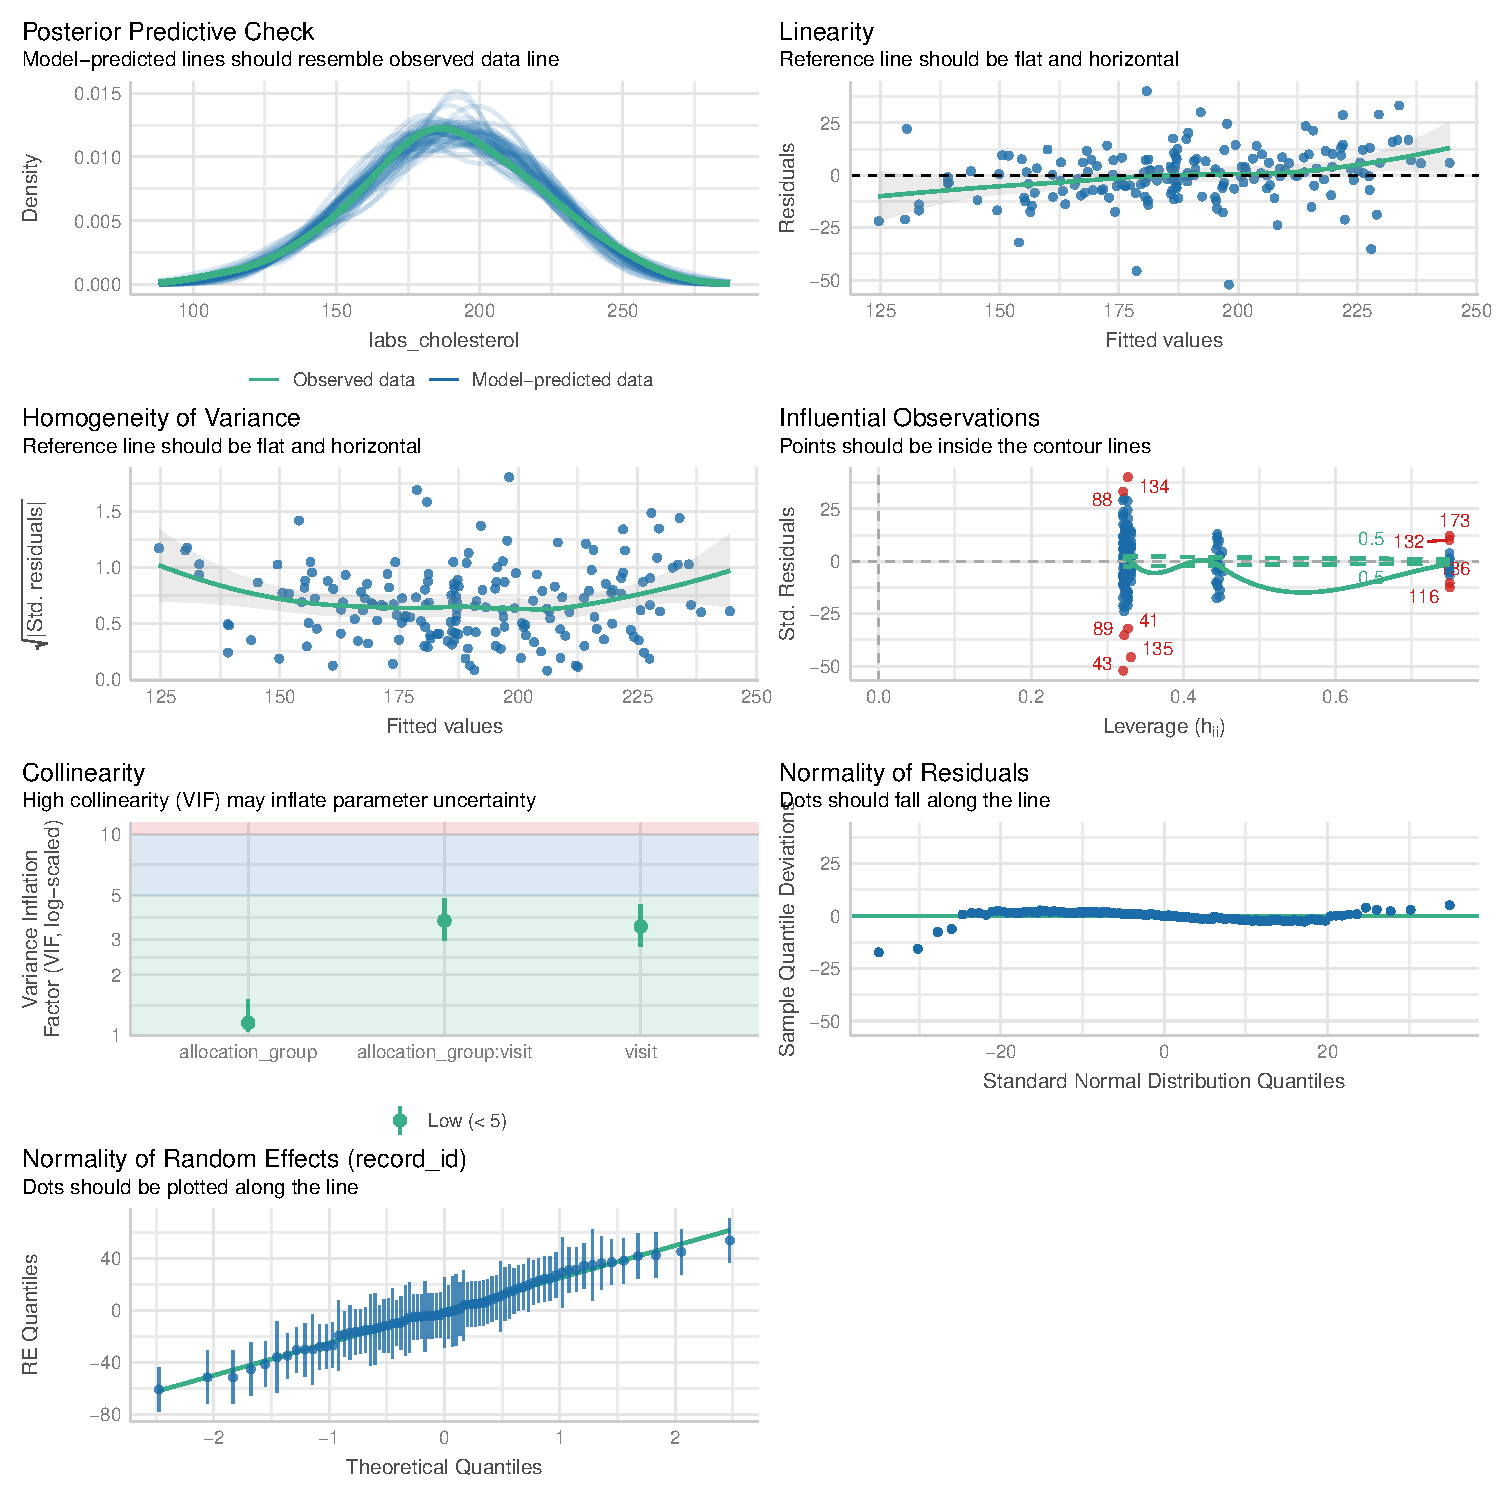
\includegraphics{Outcomes_files/figure-pdf/labs_cholesterol_4-1.pdf}

\begin{Shaded}
\begin{Highlighting}[]
\NormalTok{performance}\SpecialCharTok{::}\FunctionTok{check\_model}\NormalTok{(labs\_cholesterol\_model\_sens)}
\end{Highlighting}
\end{Shaded}

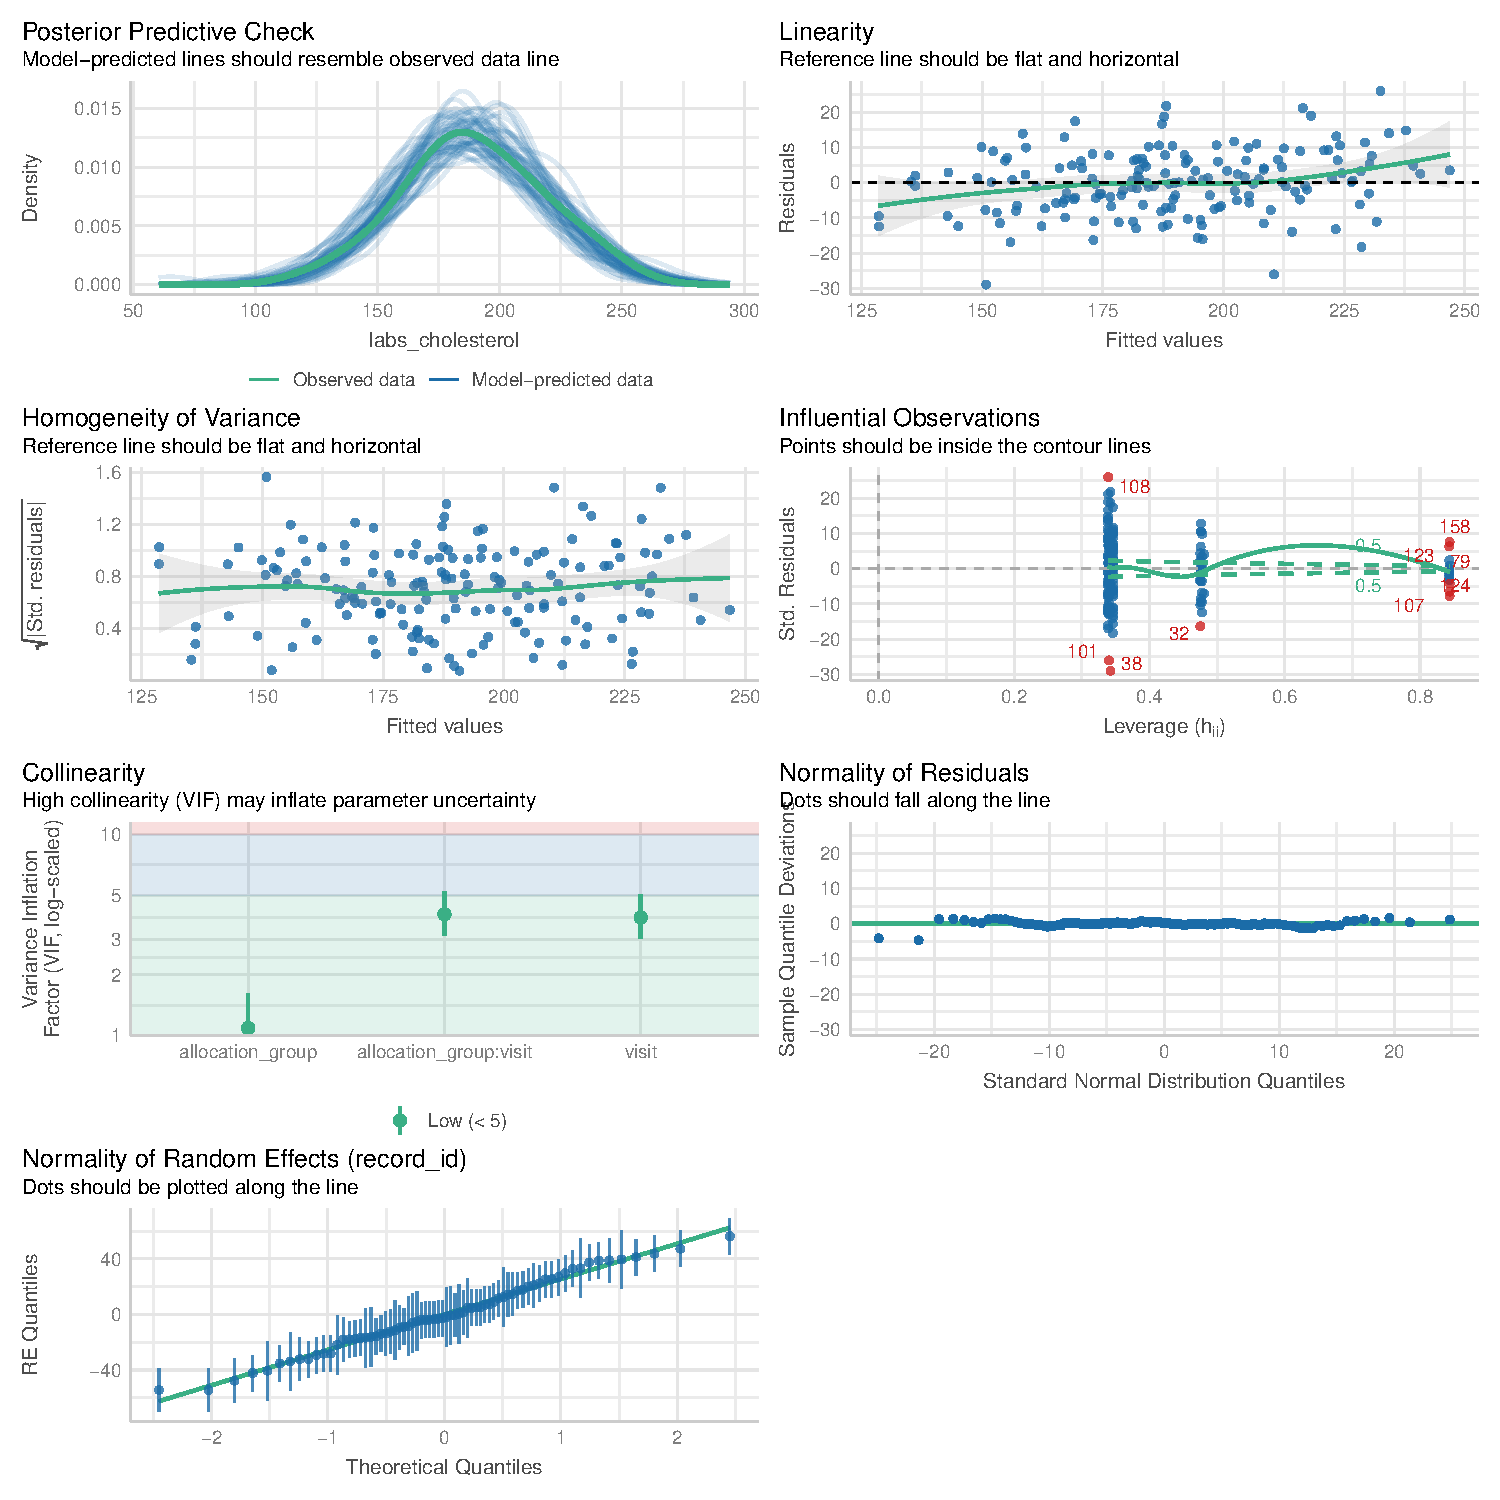
\includegraphics{Outcomes_files/figure-pdf/labs_cholesterol_4-2.pdf}

\paragraph{Médias Marginais
Estimadas}\label{muxe9dias-marginais-estimadas-4}

\subparagraph{Todos os dados}\label{todos-os-dados-4}

\begin{Shaded}
\begin{Highlighting}[]
\CommentTok{\# Get EMMs for each group at each visit}
\NormalTok{labs\_cholesterol\_raw\_emm }\OtherTok{\textless{}{-}}\NormalTok{ emmeans}\SpecialCharTok{::}\FunctionTok{emmeans}\NormalTok{(}
\NormalTok{    labs\_cholesterol\_model, }
    \SpecialCharTok{\textasciitilde{}}\NormalTok{ allocation\_group }\SpecialCharTok{*}\NormalTok{ visit}
\NormalTok{)}

\NormalTok{labs\_cholesterol\_raw\_emm }\OtherTok{\textless{}{-}} \FunctionTok{regrid}\NormalTok{(labs\_cholesterol\_raw\_emm)}

\CommentTok{\# Table of marginal means}
\CommentTok{\# labs\_cholesterol\_raw\_emm}

\CommentTok{\# Pairwise comparisons: Between groups at each visit}
\NormalTok{emmeans}\SpecialCharTok{::}\FunctionTok{contrast}\NormalTok{(labs\_cholesterol\_raw\_emm,}
\AttributeTok{method =} \StringTok{"pairwise"}\NormalTok{, }\AttributeTok{by =} \StringTok{"visit"}\NormalTok{,}
\AttributeTok{adjust =} \StringTok{"bonferroni"}\NormalTok{) }\SpecialCharTok{\%\textgreater{}\%} \FunctionTok{summary}\NormalTok{(}\AttributeTok{infer =} \FunctionTok{c}\NormalTok{(}\ConstantTok{TRUE}\NormalTok{, }\ConstantTok{TRUE}\NormalTok{))}
\end{Highlighting}
\end{Shaded}

\begin{verbatim}
visit = 1:
 contrast          estimate   SE    df lower.CL upper.CL t.ratio p.value
 Grupo A - Grupo B    0.717 7.30  95.4   -13.78     15.2   0.098  0.9221

visit = 2:
 contrast          estimate   SE    df lower.CL upper.CL t.ratio p.value
 Grupo A - Grupo B    0.832 7.81 107.2   -14.65     16.3   0.107  0.9154

visit = 3:
 contrast          estimate   SE    df lower.CL upper.CL t.ratio p.value
 Grupo A - Grupo B    8.476 8.15 121.8    -7.66     24.6   1.040  0.3004

Degrees-of-freedom method: inherited from kenward-roger when re-gridding 
Confidence level used: 0.95 
\end{verbatim}

\begin{Shaded}
\begin{Highlighting}[]
\CommentTok{\# Pairwise comparisons: Changes over time within each group}
\NormalTok{emmeans}\SpecialCharTok{::}\FunctionTok{contrast}\NormalTok{(labs\_cholesterol\_raw\_emm,}
\AttributeTok{method =} \StringTok{"pairwise"}\NormalTok{, }\AttributeTok{by =} \StringTok{"allocation\_group"}\NormalTok{,}
\AttributeTok{adjust =} \StringTok{"bonferroni"}\NormalTok{) }\SpecialCharTok{\%\textgreater{}\%} \FunctionTok{summary}\NormalTok{(}\AttributeTok{infer =} \FunctionTok{c}\NormalTok{(}\ConstantTok{TRUE}\NormalTok{, }\ConstantTok{TRUE}\NormalTok{))}
\end{Highlighting}
\end{Shaded}

\begin{verbatim}
allocation_group = Grupo A:
 contrast        estimate   SE    df lower.CL upper.CL t.ratio p.value
 visit1 - visit2     5.91 4.03  95.4    -3.92    15.73   1.465  0.4387
 visit1 - visit3     0.38 4.37  95.4   -10.27    11.03   0.087  1.0000
 visit2 - visit3    -5.53 4.41 107.2   -16.25     5.19  -1.254  0.6378

allocation_group = Grupo B:
 contrast        estimate   SE    df lower.CL upper.CL t.ratio p.value
 visit1 - visit2     6.02 4.34  95.4    -4.54    16.59   1.389  0.5041
 visit1 - visit3     8.14 4.62  95.4    -3.13    19.41   1.760  0.2448
 visit2 - visit3     2.12 4.82 121.6    -9.58    13.81   0.439  1.0000

Degrees-of-freedom method: inherited from kenward-roger when re-gridding 
Confidence level used: 0.95 
Conf-level adjustment: bonferroni method for 3 estimates 
P value adjustment: bonferroni method for 3 tests 
\end{verbatim}

\begin{Shaded}
\begin{Highlighting}[]
\CommentTok{\# Plot of marginal means}
\FunctionTok{plot}\NormalTok{(labs\_cholesterol\_raw\_emm, }\AttributeTok{comparisons =} \ConstantTok{TRUE}\NormalTok{)}
\end{Highlighting}
\end{Shaded}

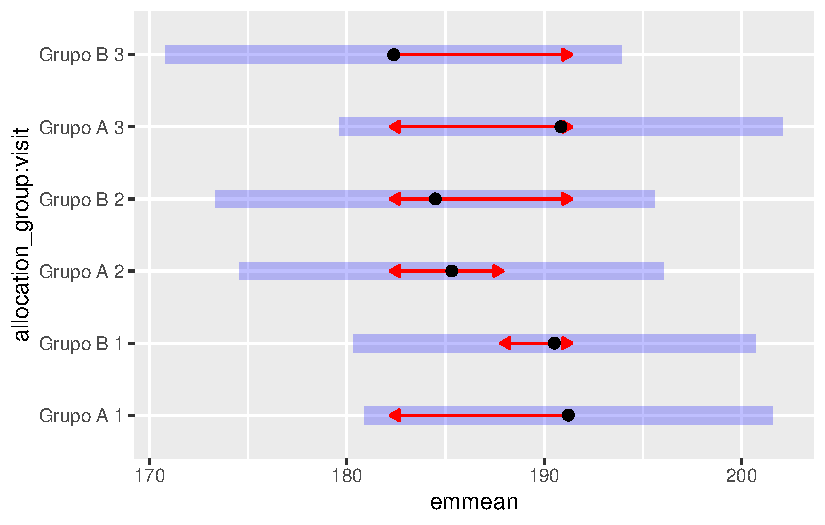
\includegraphics{Outcomes_files/figure-pdf/labs_cholesterol_raw_emm-1.pdf}

\subparagraph{Análise de
sensibilidade}\label{anuxe1lise-de-sensibilidade-4}

\begin{Shaded}
\begin{Highlighting}[]
\CommentTok{\# Get EMMs for each group at each visit (Sensitivity Analysis)}
\NormalTok{labs\_cholesterol\_emm }\OtherTok{\textless{}{-}}\NormalTok{ emmeans}\SpecialCharTok{::}\FunctionTok{emmeans}\NormalTok{(}
\NormalTok{    labs\_cholesterol\_model\_sens, }
    \SpecialCharTok{\textasciitilde{}}\NormalTok{ allocation\_group }\SpecialCharTok{*}\NormalTok{ visit}
\NormalTok{)}

\NormalTok{labs\_cholesterol\_emm }\OtherTok{\textless{}{-}} \FunctionTok{regrid}\NormalTok{(labs\_cholesterol\_emm)}

\CommentTok{\# Table of marginal means}
\CommentTok{\# labs\_cholesterol\_emm}

\CommentTok{\# Pairwise comparisons: Between groups at each visit}
\NormalTok{emmeans}\SpecialCharTok{::}\FunctionTok{contrast}\NormalTok{(labs\_cholesterol\_emm,}
\AttributeTok{method =} \StringTok{"pairwise"}\NormalTok{, }\AttributeTok{by =} \StringTok{"visit"}\NormalTok{,}
\AttributeTok{adjust =} \StringTok{"bonferroni"}\NormalTok{) }\SpecialCharTok{\%\textgreater{}\%} \FunctionTok{summary}\NormalTok{(}\AttributeTok{infer =} \FunctionTok{c}\NormalTok{(}\ConstantTok{TRUE}\NormalTok{, }\ConstantTok{TRUE}\NormalTok{))}
\end{Highlighting}
\end{Shaded}

\begin{verbatim}
visit = 1:
 contrast          estimate   SE   df lower.CL upper.CL t.ratio p.value
 Grupo A - Grupo B    0.678 7.05 79.8    -13.4     14.7   0.096  0.9237

visit = 2:
 contrast          estimate   SE   df lower.CL upper.CL t.ratio p.value
 Grupo A - Grupo B    2.235 7.40 88.6    -12.5     16.9   0.302  0.7632

visit = 3:
 contrast          estimate   SE   df lower.CL upper.CL t.ratio p.value
 Grupo A - Grupo B    2.807 7.64 99.7    -12.4     18.0   0.367  0.7142

Degrees-of-freedom method: inherited from kenward-roger when re-gridding 
Confidence level used: 0.95 
\end{verbatim}

\begin{Shaded}
\begin{Highlighting}[]
\CommentTok{\# Pairwise comparisons: Changes over time within each group}
\NormalTok{emmeans}\SpecialCharTok{::}\FunctionTok{contrast}\NormalTok{(labs\_cholesterol\_emm,}
\AttributeTok{method =} \StringTok{"pairwise"}\NormalTok{, }\AttributeTok{by =} \StringTok{"allocation\_group"}\NormalTok{,}
\AttributeTok{adjust =} \StringTok{"bonferroni"}\NormalTok{) }\SpecialCharTok{\%\textgreater{}\%} \FunctionTok{summary}\NormalTok{(}\AttributeTok{infer =} \FunctionTok{c}\NormalTok{(}\ConstantTok{TRUE}\NormalTok{, }\ConstantTok{TRUE}\NormalTok{))}
\end{Highlighting}
\end{Shaded}

\begin{verbatim}
allocation_group = Grupo A:
 contrast        estimate   SE   df lower.CL upper.CL t.ratio p.value
 visit1 - visit2     5.98 3.20 79.8   -1.832    13.80   1.872  0.1944
 visit1 - visit3     3.94 3.52 79.8   -4.665    12.54   1.119  0.7990
 visit2 - visit3    -2.05 3.54 88.6  -10.679     6.59  -0.579  1.0000

allocation_group = Grupo B:
 contrast        estimate   SE   df lower.CL upper.CL t.ratio p.value
 visit1 - visit2     7.54 3.28 79.8   -0.478    15.56   2.300  0.0723
 visit1 - visit3     6.07 3.51 79.8   -2.516    14.65   1.729  0.2632
 visit2 - visit3    -1.47 3.65 97.7  -10.355     7.41  -0.404  1.0000

Degrees-of-freedom method: inherited from kenward-roger when re-gridding 
Confidence level used: 0.95 
Conf-level adjustment: bonferroni method for 3 estimates 
P value adjustment: bonferroni method for 3 tests 
\end{verbatim}

\begin{Shaded}
\begin{Highlighting}[]
\CommentTok{\# Plot of marginal means}
\FunctionTok{plot}\NormalTok{(labs\_cholesterol\_emm, }\AttributeTok{comparisons =} \ConstantTok{TRUE}\NormalTok{)}
\end{Highlighting}
\end{Shaded}

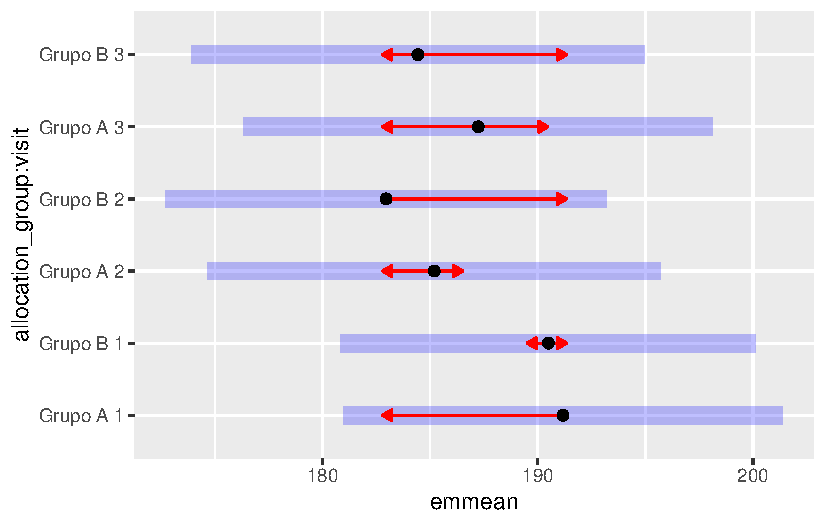
\includegraphics{Outcomes_files/figure-pdf/labs_cholesterol_sens_emm-1.pdf}

\paragraph{Resultado}\label{resultado-4}

No modelo ajustado para os níveis de colesterol total, não foram
observadas diferenças estatisticamente significativas entre os grupos em
nenhum dos três momentos avaliados. As comparações intragrupo ao longo
do tempo também não indicaram alterações significativas em nenhum dos
grupos. A análise de sensibilidade, realizada com a exclusão de
observações influentes, confirmou esses achados. As estimativas se
mantiveram estáveis e as diferenças permaneceram não significativas. As
estimativas, intervalos de confiança de 95\% e valores de p estão
apresentados na Tabela~\ref{tbl-cholesterol}.

\begin{longtable}[]{@{}
  >{\raggedright\arraybackslash}p{(\columnwidth - 8\tabcolsep) * \real{0.2000}}
  >{\raggedright\arraybackslash}p{(\columnwidth - 8\tabcolsep) * \real{0.2000}}
  >{\raggedright\arraybackslash}p{(\columnwidth - 8\tabcolsep) * \real{0.2000}}
  >{\raggedright\arraybackslash}p{(\columnwidth - 8\tabcolsep) * \real{0.2000}}
  >{\raggedright\arraybackslash}p{(\columnwidth - 8\tabcolsep) * \real{0.2000}}@{}}
\caption{Diferenças estimadas dos níveis de Colesterol Total entre os
grupos de alocação (placebo vs Eclipta) e entre visitas dentro de cada
grupo}\label{tbl-cholesterol}\tabularnewline
\toprule\noalign{}
\begin{minipage}[b]{\linewidth}\raggedright
Grupo de comparação
\end{minipage} & \begin{minipage}[b]{\linewidth}\raggedright
Comparação
\end{minipage} & \begin{minipage}[b]{\linewidth}\raggedright
Estimativa
\end{minipage} & \begin{minipage}[b]{\linewidth}\raggedright
IC 95\%
\end{minipage} & \begin{minipage}[b]{\linewidth}\raggedright
p-valor
\end{minipage} \\
\midrule\noalign{}
\endfirsthead
\toprule\noalign{}
\begin{minipage}[b]{\linewidth}\raggedright
Grupo de comparação
\end{minipage} & \begin{minipage}[b]{\linewidth}\raggedright
Comparação
\end{minipage} & \begin{minipage}[b]{\linewidth}\raggedright
Estimativa
\end{minipage} & \begin{minipage}[b]{\linewidth}\raggedright
IC 95\%
\end{minipage} & \begin{minipage}[b]{\linewidth}\raggedright
p-valor
\end{minipage} \\
\midrule\noalign{}
\endhead
\bottomrule\noalign{}
\endlastfoot
Entre grupos & Visita 1 & 0,72 & {[}-13,78 ; 15,21{]} & 0,922 \\
Entre grupos & Visita 2 & 0,83 & {[}-14,65 ; 16,30{]} & 0,915 \\
Entre grupos & Visita 3 & 8,48 & {[}-7,66 ; 24,61{]} & 0,300 \\
Grupo Placebo & Visita 1 - Visita 2 & 5,91 & {[}-3,92 ; 15,73{]} &
0,439 \\
Grupo Placebo & Visita 1 - Visita 3 & 0,38 & {[}-10,27 ; 11,03{]} &
1,000 \\
Grupo Placebo & Visita 2 - Visita 3 & -5,53 & {[}-16,25 ; 5,19{]} &
0,638 \\
Grupo Eclipta & Visita 1 - Visita 2 & 6,02 & {[}-4,54 ; 16,59{]} &
0,504 \\
Grupo Eclipta & Visita 1 - Visita 3 & 8,14 & {[}-3,13 ; 19,41{]} &
0,245 \\
Grupo Eclipta & Visita 2 - Visita 3 & 2,12 & {[}-9,58 ; 13,81{]} &
1,000 \\
\end{longtable}

\begin{Shaded}
\begin{Highlighting}[]
\FunctionTok{ggplot}\NormalTok{(}
    \AttributeTok{data =}\NormalTok{ data\_model, }
    \FunctionTok{aes}\NormalTok{(}
        \AttributeTok{x =} \FunctionTok{as.factor}\NormalTok{(visit),}
        \AttributeTok{y =}\NormalTok{ labs\_cholesterol,}
        \AttributeTok{group =}\NormalTok{ record\_id,}
\NormalTok{    )}
\NormalTok{) }\SpecialCharTok{+}
    \FunctionTok{geom\_line}\NormalTok{(}\AttributeTok{alpha =} \FloatTok{0.5}\NormalTok{) }\SpecialCharTok{+}
    \FunctionTok{geom\_point}\NormalTok{(}\AttributeTok{alpha =} \FloatTok{0.7}\NormalTok{) }\SpecialCharTok{+}
    \FunctionTok{geom\_smooth}\NormalTok{(}
        \FunctionTok{aes}\NormalTok{(}\AttributeTok{group =}\NormalTok{ allocation\_group),}
        \AttributeTok{method =} \StringTok{"lm"}\NormalTok{,}
        \AttributeTok{se =} \ConstantTok{TRUE}\NormalTok{,}
        \AttributeTok{linewidth =} \DecValTok{1}
\NormalTok{    ) }\SpecialCharTok{+}
    \FunctionTok{labs}\NormalTok{(}\AttributeTok{title =} \StringTok{"All data"}\NormalTok{) }\SpecialCharTok{+}
    \FunctionTok{facet\_wrap}\NormalTok{(}\SpecialCharTok{\textasciitilde{}}\NormalTok{ allocation\_group) }
\end{Highlighting}
\end{Shaded}

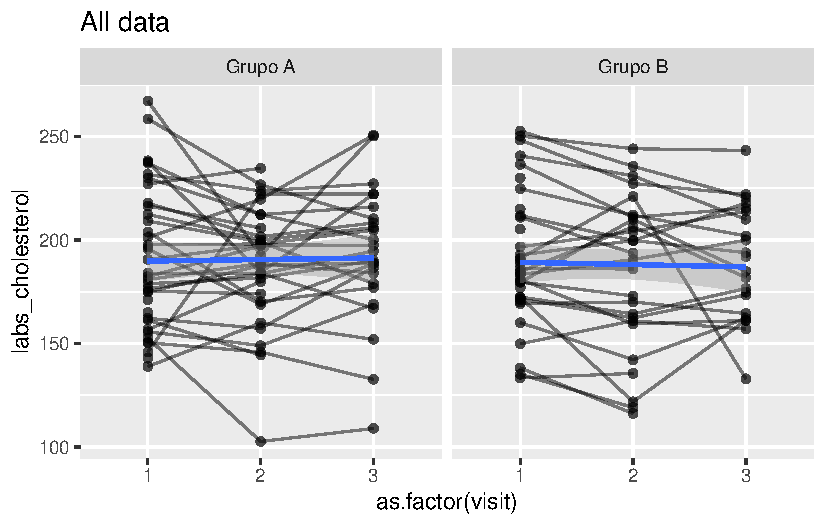
\includegraphics{Outcomes_files/figure-pdf/labs_cholesterol_6-1.pdf}

\begin{Shaded}
\begin{Highlighting}[]
    \CommentTok{\#coord\_cartesian(ylim = c(10, 150))}

\NormalTok{data\_model }\SpecialCharTok{\%\textgreater{}\%} 
    \FunctionTok{filter}\NormalTok{(}
        \SpecialCharTok{!}\NormalTok{(record\_id }\SpecialCharTok{\%in\%} 
\NormalTok{        labs\_cholesterol\_model\_check}\SpecialCharTok{$}\NormalTok{influential\_ids)}
\NormalTok{    ) }\SpecialCharTok{\%\textgreater{}\%} 
    \FunctionTok{ggplot}\NormalTok{(}
        \FunctionTok{aes}\NormalTok{(}
            \AttributeTok{x =} \FunctionTok{as.factor}\NormalTok{(visit),}
            \AttributeTok{y =}\NormalTok{ labs\_cholesterol,}
            \AttributeTok{group =}\NormalTok{ record\_id,}
\NormalTok{        )}
\NormalTok{    ) }\SpecialCharTok{+}
    \FunctionTok{geom\_line}\NormalTok{(}\AttributeTok{alpha =} \FloatTok{0.5}\NormalTok{) }\SpecialCharTok{+}
    \FunctionTok{geom\_point}\NormalTok{(}\AttributeTok{alpha =} \FloatTok{0.7}\NormalTok{) }\SpecialCharTok{+}
    \FunctionTok{geom\_smooth}\NormalTok{(}
        \FunctionTok{aes}\NormalTok{(}\AttributeTok{group =}\NormalTok{ allocation\_group),}
        \AttributeTok{method =} \StringTok{"lm"}\NormalTok{,}
        \AttributeTok{se =} \ConstantTok{TRUE}\NormalTok{,}
        \AttributeTok{linewidth =} \DecValTok{1}
\NormalTok{    ) }\SpecialCharTok{+}
    \FunctionTok{labs}\NormalTok{(}\AttributeTok{title =} \StringTok{"Sensitivity analysis"}\NormalTok{) }\SpecialCharTok{+}
    \FunctionTok{facet\_wrap}\NormalTok{(}\SpecialCharTok{\textasciitilde{}}\NormalTok{ allocation\_group) }
\end{Highlighting}
\end{Shaded}

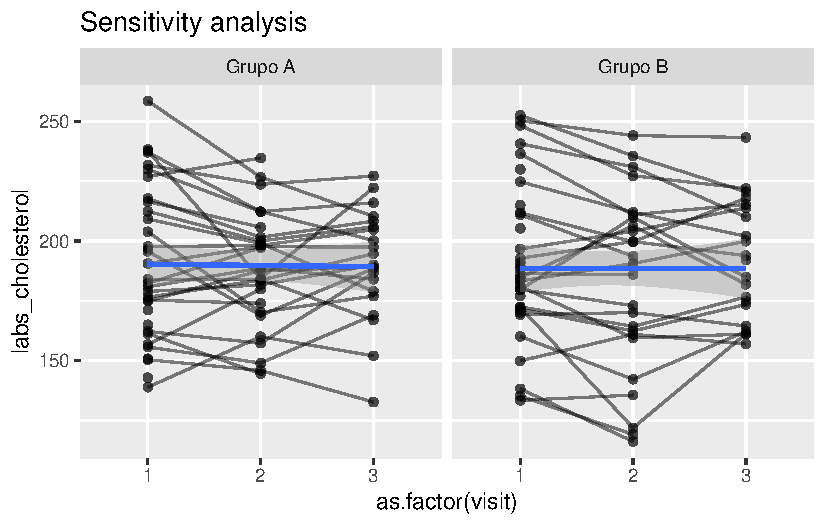
\includegraphics{Outcomes_files/figure-pdf/labs_cholesterol_6-2.pdf}

\begin{Shaded}
\begin{Highlighting}[]
    \CommentTok{\#coord\_cartesian(ylim = c(10, 150))}
\end{Highlighting}
\end{Shaded}

\subsubsection{LDL Colesterol}\label{ldl-colesterol}

Variável: \texttt{labs\_ldl}

\begin{Shaded}
\begin{Highlighting}[]
\CommentTok{\# Plot 1: Raw data}
\NormalTok{labs\_ldl\_hist\_1 }\OtherTok{\textless{}{-}}\NormalTok{ data\_model }\SpecialCharTok{\%\textgreater{}\%} 
    \CommentTok{\#filter(}
    \CommentTok{\#    labs\_ldl \textless{} 300}
    \CommentTok{\#) \%\textgreater{}\% }
    \FunctionTok{ggplot}\NormalTok{(}\FunctionTok{aes}\NormalTok{(}\AttributeTok{x =}\NormalTok{ labs\_ldl)) }\SpecialCharTok{+} 
    \FunctionTok{geom\_histogram}\NormalTok{(}\AttributeTok{bins =} \DecValTok{50}\NormalTok{, }\AttributeTok{fill =} \StringTok{"skyblue"}\NormalTok{, }\AttributeTok{color =} \StringTok{"black"}\NormalTok{)}

\CommentTok{\# Plot 2: Log{-}transformed data}
\NormalTok{labs\_ldl\_hist\_2 }\OtherTok{\textless{}{-}}\NormalTok{ data\_model }\SpecialCharTok{\%\textgreater{}\%} 
    \CommentTok{\#filter(}
    \CommentTok{\#    labs\_ldl \textless{} 300}
    \CommentTok{\#) \%\textgreater{}\%}
    \FunctionTok{ggplot}\NormalTok{(}\FunctionTok{aes}\NormalTok{(}\AttributeTok{x =} \FunctionTok{log1p}\NormalTok{(labs\_ldl))) }\SpecialCharTok{+} 
    \FunctionTok{geom\_histogram}\NormalTok{(}\AttributeTok{bins =} \DecValTok{50}\NormalTok{, }\AttributeTok{fill =} \StringTok{"lightgreen"}\NormalTok{, }\AttributeTok{color =} \StringTok{"black"}\NormalTok{)}

\CommentTok{\# Combine side by side}
\NormalTok{labs\_ldl\_hist\_1 }\SpecialCharTok{+}\NormalTok{ labs\_ldl\_hist\_2 }\CommentTok{\# library(patchwork)}
\end{Highlighting}
\end{Shaded}

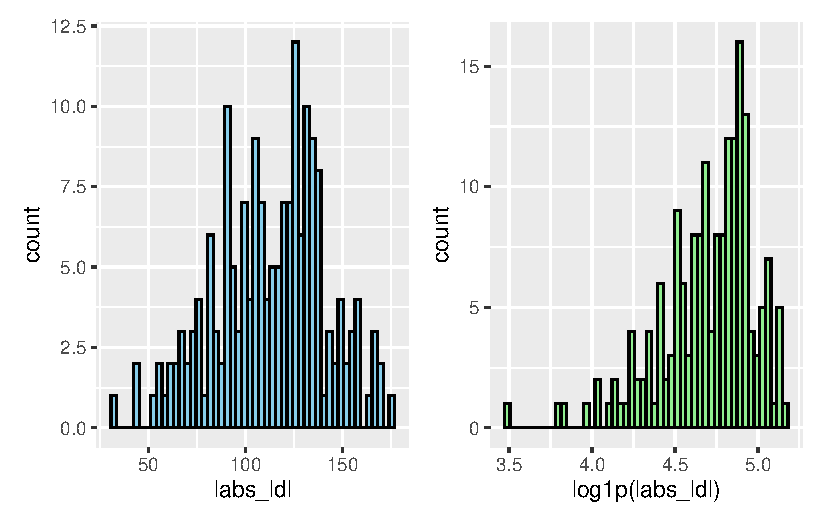
\includegraphics{Outcomes_files/figure-pdf/labs_ldl_1-1.pdf}

\begin{Shaded}
\begin{Highlighting}[]
\CommentTok{\# LMM}
\NormalTok{labs\_ldl\_model }\OtherTok{\textless{}{-}} \FunctionTok{lmer}\NormalTok{(labs\_ldl }\SpecialCharTok{\textasciitilde{}}\NormalTok{ allocation\_group }\SpecialCharTok{*}\NormalTok{ visit }\SpecialCharTok{+} 
\NormalTok{(}\DecValTok{1} \SpecialCharTok{|}\NormalTok{ record\_id), }\AttributeTok{data =}\NormalTok{ data\_model)}
\FunctionTok{check\_collinearity}\NormalTok{(labs\_ldl\_model)}
\end{Highlighting}
\end{Shaded}

\begin{verbatim}
# Check for Multicollinearity

Low Correlation

                   Term  VIF   VIF 95% CI Increased SE Tolerance Tolerance 95% CI
       allocation_group 1.18 [1.06, 1.52]         1.08      0.85     [0.66, 0.94]
                  visit 3.49 [2.78, 4.49]         1.87      0.29     [0.22, 0.36]
 allocation_group:visit 3.77 [3.00, 4.86]         1.94      0.26     [0.21, 0.33]
\end{verbatim}

\begin{Shaded}
\begin{Highlighting}[]
\CommentTok{\# Sensitivity analysis}
\NormalTok{labs\_ldl\_model\_check }\OtherTok{\textless{}{-}} \FunctionTok{sensitivity\_check\_lmer}\NormalTok{(}
    \AttributeTok{model =}\NormalTok{ labs\_ldl\_model,}
    \AttributeTok{id\_var =} \StringTok{"record\_id"}\NormalTok{,}
    \AttributeTok{top\_n =} \DecValTok{7}\NormalTok{)}

\CommentTok{\# LMM Sensitivity}
\NormalTok{labs\_ldl\_model\_sens }\OtherTok{\textless{}{-}} \FunctionTok{update}\NormalTok{(}\AttributeTok{object =}\NormalTok{ labs\_ldl\_model,}
                              \AttributeTok{subset =} \SpecialCharTok{!}\NormalTok{(record\_id }\SpecialCharTok{\%in\%} 
\NormalTok{        labs\_ldl\_model\_check}\SpecialCharTok{$}\NormalTok{influential\_ids))}
\CommentTok{\# Influential IDS}
\NormalTok{labs\_ldl\_model\_check}\SpecialCharTok{$}\NormalTok{influential\_ids}
\end{Highlighting}
\end{Shaded}

\begin{verbatim}
[1] "16" "17" "56" "37" "50" "61" "75"
\end{verbatim}

\paragraph{Resumo dos modelos}\label{resumo-dos-modelos-5}

\begin{Shaded}
\begin{Highlighting}[]
\CommentTok{\# Model comparison}
\FunctionTok{summary}\NormalTok{(labs\_ldl\_model)}
\end{Highlighting}
\end{Shaded}

\begin{verbatim}
Linear mixed model fit by REML. t-tests use Satterthwaite's method ['lmerModLmerTest']
Formula: labs_ldl ~ allocation_group * visit + (1 | record_id)
   Data: data_model

REML criterion at convergence: 1601.5

Scaled residuals: 
    Min      1Q  Median      3Q     Max 
-2.9892 -0.3229 -0.0296  0.3610  2.5195 

Random effects:
 Groups    Name        Variance Std.Dev.
 record_id (Intercept) 605.7    24.61   
 Residual              249.7    15.80   
Number of obs: 179, groups:  record_id, 75

Fixed effects:
                               Estimate Std. Error       df t value Pr(>|t|)    
(Intercept)                    115.4919     4.8081  98.3445  24.020   <2e-16 ***
allocation_groupGrupo B         -3.7735     6.7548  98.3445  -0.559    0.578    
visit2                          -5.5925     3.9659 103.9503  -1.410    0.161    
visit3                          -0.0205     4.2968 105.1671  -0.005    0.996    
allocation_groupGrupo B:visit2   1.9191     5.8182 105.6037   0.330    0.742    
allocation_groupGrupo B:visit3  -5.9060     6.2502 106.5086  -0.945    0.347    
---
Signif. codes:  0 '***' 0.001 '**' 0.01 '*' 0.05 '.' 0.1 ' ' 1

Correlation of Fixed Effects:
            (Intr) all_GB visit2 visit3 a_GB:2
allctn_grGB -0.712                            
visit2      -0.354  0.252                     
visit3      -0.327  0.233  0.450              
allctn_GB:2  0.241 -0.339 -0.682 -0.307       
allctn_GB:3  0.225 -0.315 -0.310 -0.687  0.434
\end{verbatim}

\begin{Shaded}
\begin{Highlighting}[]
\FunctionTok{summary}\NormalTok{(labs\_ldl\_model\_sens)}
\end{Highlighting}
\end{Shaded}

\begin{verbatim}
Linear mixed model fit by REML. t-tests use Satterthwaite's method ['lmerModLmerTest']
Formula: labs_ldl ~ allocation_group * visit + (1 | record_id)
   Data: data_model
 Subset: !(record_id %in% labs_ldl_model_check$influential_ids)

REML criterion at convergence: 1338.9

Scaled residuals: 
     Min       1Q   Median       3Q      Max 
-1.83006 -0.44200 -0.05731  0.40788  2.36163 

Random effects:
 Groups    Name        Variance Std.Dev.
 record_id (Intercept) 650.2    25.50   
 Residual              111.8    10.57   
Number of obs: 158, groups:  record_id, 68

Fixed effects:
                               Estimate Std. Error       df t value Pr(>|t|)    
(Intercept)                    115.8687     4.8799  75.3685  23.744   <2e-16 ***
allocation_groupGrupo B         -3.8299     6.7068  75.3685  -0.571   0.5697    
visit2                          -5.1922     2.9125  87.5739  -1.783   0.0781 .  
visit3                           0.6698     3.2198  88.0305   0.208   0.8357    
allocation_groupGrupo B:visit2   1.8681     4.1755  88.1990   0.447   0.6557    
allocation_groupGrupo B:visit3  -5.5726     4.5483  88.5080  -1.225   0.2237    
---
Signif. codes:  0 '***' 0.001 '**' 0.01 '*' 0.05 '.' 0.1 ' ' 1

Correlation of Fixed Effects:
            (Intr) all_GB visit2 visit3 a_GB:2
allctn_grGB -0.728                            
visit2      -0.246  0.179                     
visit3      -0.222  0.162  0.446              
allctn_GB:2  0.171 -0.236 -0.698 -0.311       
allctn_GB:3  0.157 -0.216 -0.316 -0.708  0.434
\end{verbatim}

\begin{Shaded}
\begin{Highlighting}[]
\NormalTok{labs\_ldl\_model\_check}\SpecialCharTok{$}\NormalTok{comparison\_table}
\end{Highlighting}
\end{Shaded}

\begin{verbatim}
# A tibble: 16 x 6
   Model       term                           estimate std.error statistic   p.value
   <chr>       <chr>                             <dbl>     <dbl>     <dbl>     <dbl>
 1 Original    (Intercept)                    115.          4.81  24.0      6.20e-43
 2 Sensitivity (Intercept)                    116.          4.88  23.7      1.00e-36
 3 Original    allocation_groupGrupo B         -3.77        6.75  -0.559    5.78e- 1
 4 Sensitivity allocation_groupGrupo B         -3.83        6.71  -0.571    5.70e- 1
 5 Original    allocation_groupGrupo B:visit2   1.92        5.82   0.330    7.42e- 1
 6 Sensitivity allocation_groupGrupo B:visit2   1.87        4.18   0.447    6.56e- 1
 7 Original    allocation_groupGrupo B:visit3  -5.91        6.25  -0.945    3.47e- 1
 8 Sensitivity allocation_groupGrupo B:visit3  -5.57        4.55  -1.23     2.24e- 1
 9 Original    sd__(Intercept)                 24.6        NA     NA       NA       
10 Sensitivity sd__(Intercept)                 25.5        NA     NA       NA       
11 Original    sd__Observation                 15.8        NA     NA       NA       
12 Sensitivity sd__Observation                 10.6        NA     NA       NA       
13 Original    visit2                          -5.59        3.97  -1.41     1.61e- 1
14 Sensitivity visit2                          -5.19        2.91  -1.78     7.81e- 2
15 Original    visit3                          -0.0205      4.30  -0.00477  9.96e- 1
16 Sensitivity visit3                           0.670       3.22   0.208    8.36e- 1
\end{verbatim}

\begin{Shaded}
\begin{Highlighting}[]
\NormalTok{performance}\SpecialCharTok{::}\FunctionTok{compare\_performance}\NormalTok{(}
\NormalTok{    labs\_ldl\_model, }
\NormalTok{    labs\_ldl\_model\_sens) }
\end{Highlighting}
\end{Shaded}

\begin{verbatim}
# Comparison of Model Performance Indices

Name                |           Model |  AIC (weights) | AICc (weights) |  BIC (weights) | R2 (cond.) | R2 (marg.) |   ICC |   RMSE |  Sigma
--------------------------------------------------------------------------------------------------------------------------------------------
labs_ldl_model      | lmerModLmerTest | 1645.5 (<.001) | 1646.4 (<.001) | 1671.0 (<.001) |      0.712 |      0.014 | 0.708 | 12.514 | 15.802
labs_ldl_model_sens | lmerModLmerTest | 1380.5 (>.999) | 1381.5 (>.999) | 1405.0 (>.999) |      0.855 |      0.014 | 0.853 |  8.043 | 10.574
\end{verbatim}

\begin{Shaded}
\begin{Highlighting}[]
\NormalTok{performance}\SpecialCharTok{::}\FunctionTok{check\_model}\NormalTok{(labs\_ldl\_model)}
\end{Highlighting}
\end{Shaded}

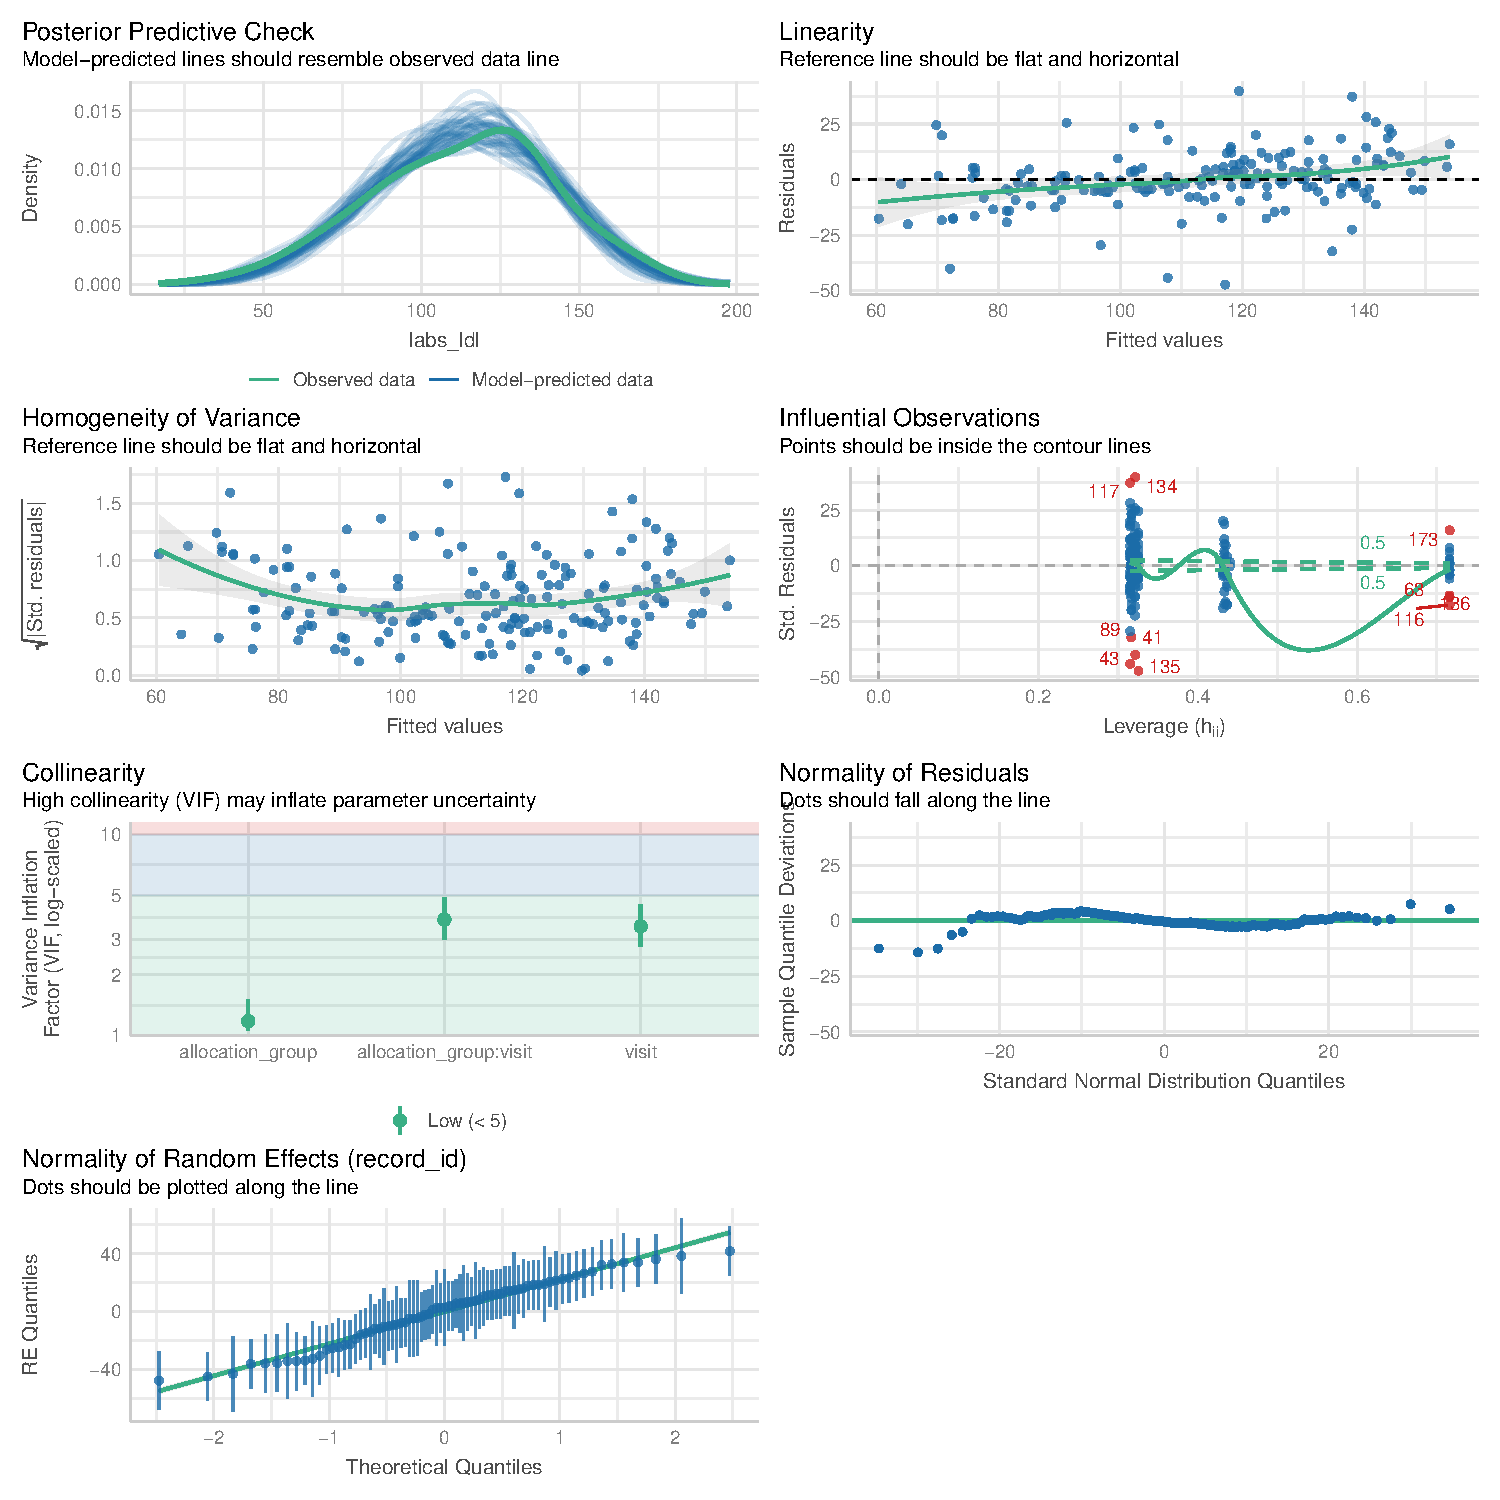
\includegraphics{Outcomes_files/figure-pdf/labs_ldl_4-1.pdf}

\begin{Shaded}
\begin{Highlighting}[]
\NormalTok{performance}\SpecialCharTok{::}\FunctionTok{check\_model}\NormalTok{(labs\_ldl\_model\_sens)}
\end{Highlighting}
\end{Shaded}

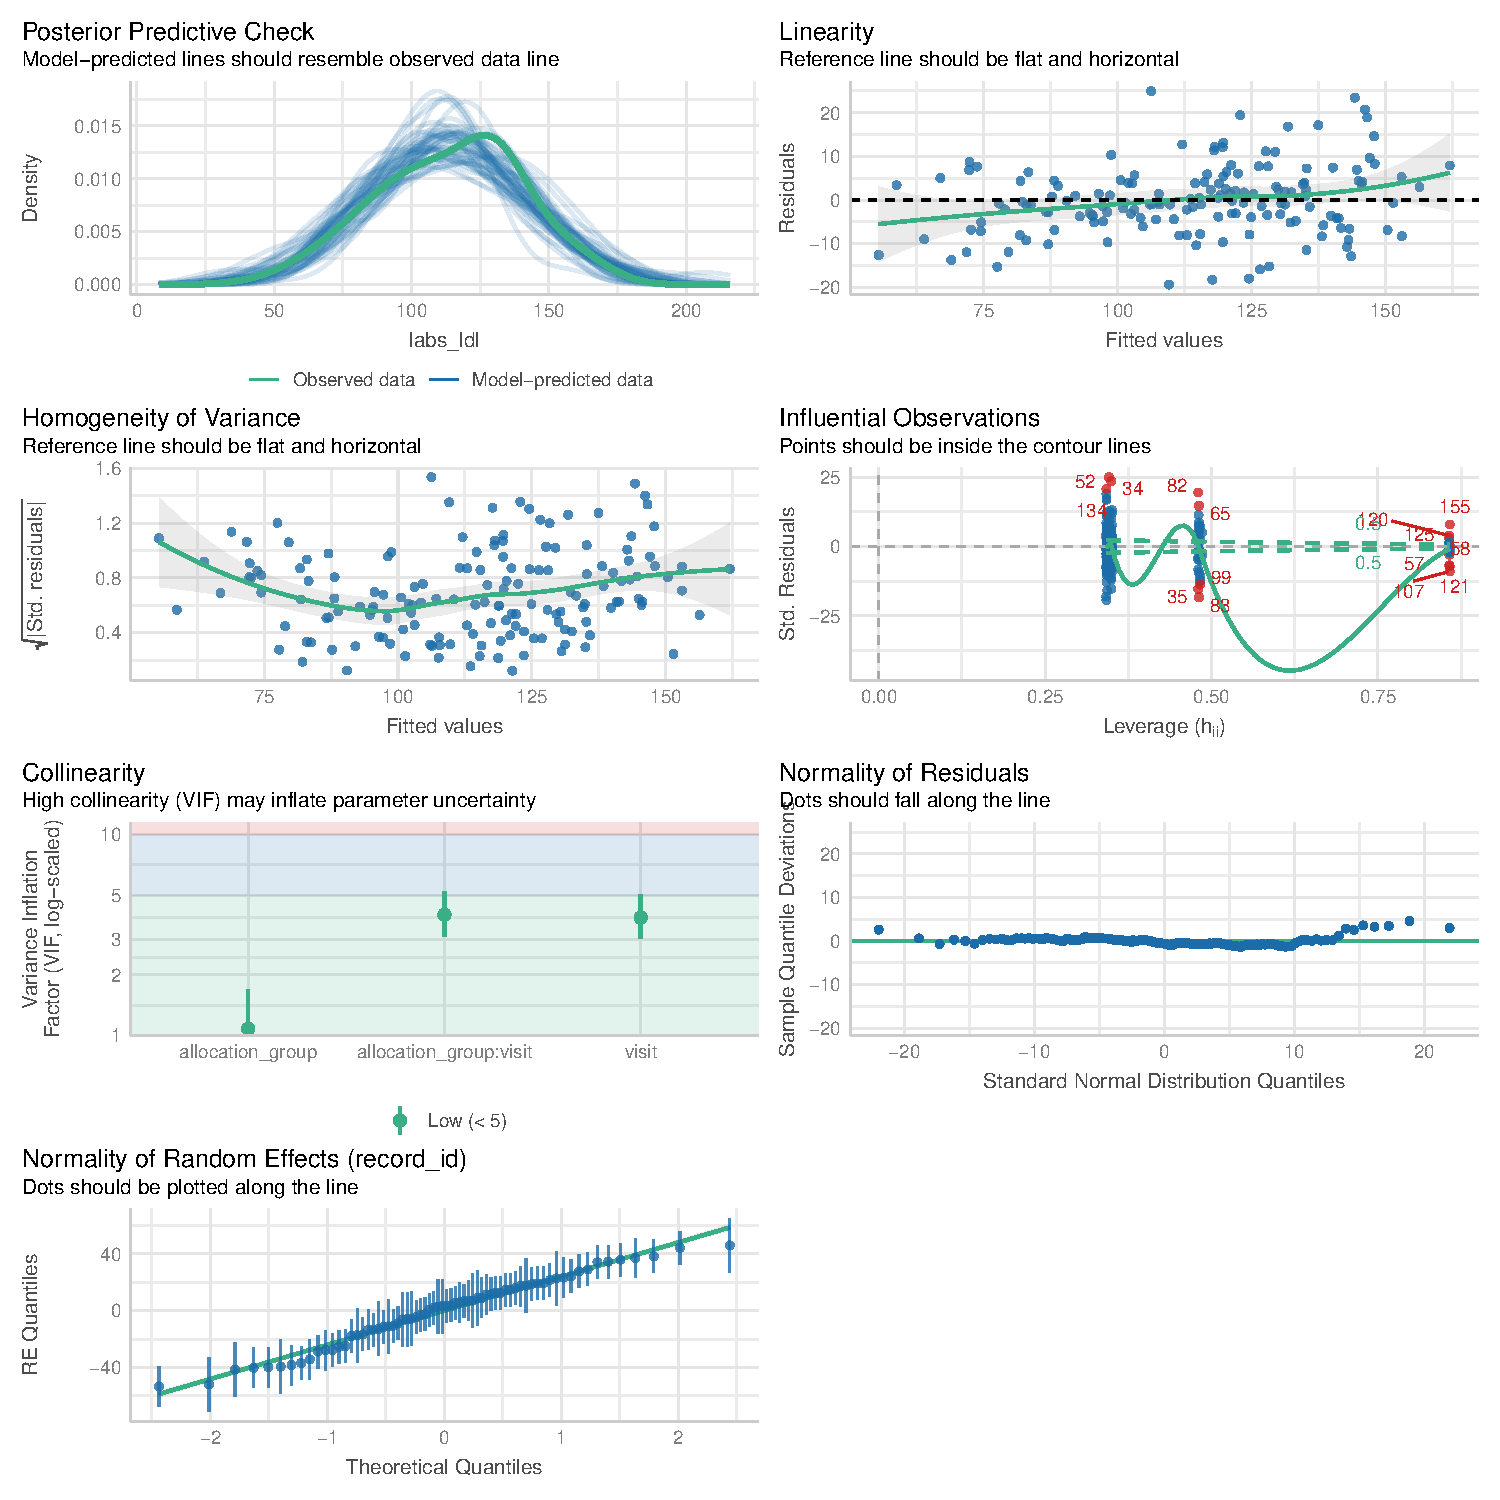
\includegraphics{Outcomes_files/figure-pdf/labs_ldl_4-2.pdf}

\paragraph{Médias Marginais
Estimadas}\label{muxe9dias-marginais-estimadas-5}

\subparagraph{Todos os dados}\label{todos-os-dados-5}

\begin{Shaded}
\begin{Highlighting}[]
\CommentTok{\# Get EMMs for each group at each visit}
\NormalTok{labs\_ldl\_raw\_emm }\OtherTok{\textless{}{-}}\NormalTok{ emmeans}\SpecialCharTok{::}\FunctionTok{emmeans}\NormalTok{(}
\NormalTok{    labs\_ldl\_model, }
    \SpecialCharTok{\textasciitilde{}}\NormalTok{ allocation\_group }\SpecialCharTok{*}\NormalTok{ visit}
\NormalTok{)}

\NormalTok{labs\_ldl\_raw\_emm }\OtherTok{\textless{}{-}} \FunctionTok{regrid}\NormalTok{(labs\_ldl\_raw\_emm)}

\CommentTok{\# Table of marginal means}
\CommentTok{\# labs\_ldl\_raw\_emm}

\CommentTok{\# Pairwise comparisons: Between groups at each visit}
\NormalTok{emmeans}\SpecialCharTok{::}\FunctionTok{contrast}\NormalTok{(labs\_ldl\_raw\_emm,}
\AttributeTok{method =} \StringTok{"pairwise"}\NormalTok{, }\AttributeTok{by =} \StringTok{"visit"}\NormalTok{,}
\AttributeTok{adjust =} \StringTok{"bonferroni"}\NormalTok{) }\SpecialCharTok{\%\textgreater{}\%} \FunctionTok{summary}\NormalTok{(}\AttributeTok{infer =} \FunctionTok{c}\NormalTok{(}\ConstantTok{TRUE}\NormalTok{, }\ConstantTok{TRUE}\NormalTok{))}
\end{Highlighting}
\end{Shaded}

\begin{verbatim}
visit = 1:
 contrast          estimate   SE    df lower.CL upper.CL t.ratio p.value
 Grupo A - Grupo B     3.77 6.75  99.1    -9.63     17.2   0.559  0.5777

visit = 2:
 contrast          estimate   SE    df lower.CL upper.CL t.ratio p.value
 Grupo A - Grupo B     1.85 7.27 111.9   -12.56     16.3   0.255  0.7993

visit = 3:
 contrast          estimate   SE    df lower.CL upper.CL t.ratio p.value
 Grupo A - Grupo B     9.68 7.63 127.7    -5.41     24.8   1.269  0.2067

Degrees-of-freedom method: inherited from kenward-roger when re-gridding 
Confidence level used: 0.95 
\end{verbatim}

\begin{Shaded}
\begin{Highlighting}[]
\CommentTok{\# Pairwise comparisons: Changes over time within each group}
\NormalTok{emmeans}\SpecialCharTok{::}\FunctionTok{contrast}\NormalTok{(labs\_ldl\_raw\_emm,}
\AttributeTok{method =} \StringTok{"pairwise"}\NormalTok{, }\AttributeTok{by =} \StringTok{"allocation\_group"}\NormalTok{,}
\AttributeTok{adjust =} \StringTok{"bonferroni"}\NormalTok{) }\SpecialCharTok{\%\textgreater{}\%} \FunctionTok{summary}\NormalTok{(}\AttributeTok{infer =} \FunctionTok{c}\NormalTok{(}\ConstantTok{TRUE}\NormalTok{, }\ConstantTok{TRUE}\NormalTok{))}
\end{Highlighting}
\end{Shaded}

\begin{verbatim}
allocation_group = Grupo A:
 contrast        estimate   SE    df lower.CL upper.CL t.ratio p.value
 visit1 - visit2   5.5925 3.97  99.1    -4.07    15.26   1.409  0.4859
 visit1 - visit3   0.0205 4.30  99.1   -10.46    10.50   0.005  1.0000
 visit2 - visit3  -5.5720 4.34 111.9   -16.13     4.98  -1.283  0.6064

allocation_group = Grupo B:
 contrast        estimate   SE    df lower.CL upper.CL t.ratio p.value
 visit1 - visit2   3.6734 4.26  99.1    -6.71    14.06   0.862  1.0000
 visit1 - visit3   5.9265 4.55  99.1    -5.15    17.00   1.304  0.5862
 visit2 - visit3   2.2531 4.74 127.2    -9.26    13.76   0.475  1.0000

Degrees-of-freedom method: inherited from kenward-roger when re-gridding 
Confidence level used: 0.95 
Conf-level adjustment: bonferroni method for 3 estimates 
P value adjustment: bonferroni method for 3 tests 
\end{verbatim}

\begin{Shaded}
\begin{Highlighting}[]
\CommentTok{\# Plot of marginal means}
\FunctionTok{plot}\NormalTok{(labs\_ldl\_raw\_emm, }\AttributeTok{comparisons =} \ConstantTok{TRUE}\NormalTok{)}
\end{Highlighting}
\end{Shaded}

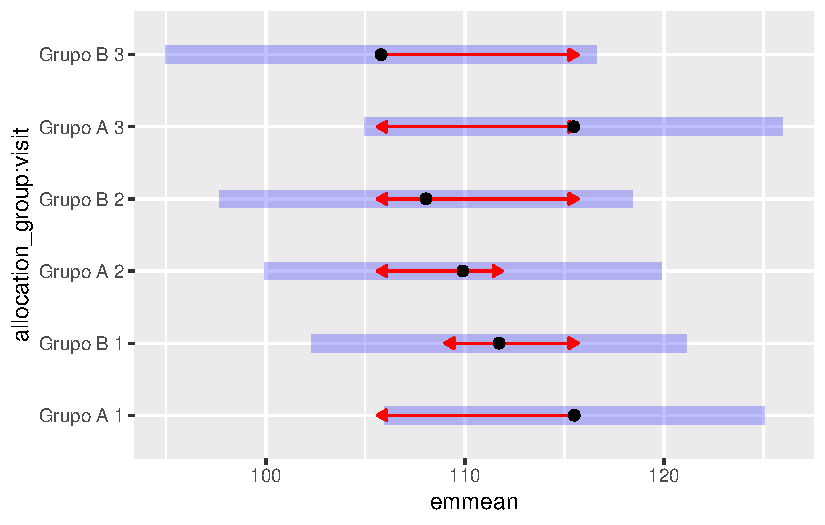
\includegraphics{Outcomes_files/figure-pdf/labs_ldl_raw_emm-1.pdf}

\subparagraph{Análise de
sensibilidade}\label{anuxe1lise-de-sensibilidade-5}

\begin{Shaded}
\begin{Highlighting}[]
\CommentTok{\# Get EMMs for each group at each visit (Sensitivity Analysis)}
\NormalTok{labs\_ldl\_emm }\OtherTok{\textless{}{-}}\NormalTok{ emmeans}\SpecialCharTok{::}\FunctionTok{emmeans}\NormalTok{(}
\NormalTok{    labs\_ldl\_model\_sens, }
    \SpecialCharTok{\textasciitilde{}}\NormalTok{ allocation\_group }\SpecialCharTok{*}\NormalTok{ visit}
\NormalTok{)}

\NormalTok{labs\_ldl\_emm }\OtherTok{\textless{}{-}} \FunctionTok{regrid}\NormalTok{(labs\_ldl\_emm)}

\CommentTok{\# Table of marginal means}
\CommentTok{\# labs\_ldl\_emm}

\CommentTok{\# Pairwise comparisons: Between groups at each visit}
\NormalTok{emmeans}\SpecialCharTok{::}\FunctionTok{contrast}\NormalTok{(labs\_ldl\_emm,}
\AttributeTok{method =} \StringTok{"pairwise"}\NormalTok{, }\AttributeTok{by =} \StringTok{"visit"}\NormalTok{,}
\AttributeTok{adjust =} \StringTok{"bonferroni"}\NormalTok{) }\SpecialCharTok{\%\textgreater{}\%} \FunctionTok{summary}\NormalTok{(}\AttributeTok{infer =} \FunctionTok{c}\NormalTok{(}\ConstantTok{TRUE}\NormalTok{, }\ConstantTok{TRUE}\NormalTok{))}
\end{Highlighting}
\end{Shaded}

\begin{verbatim}
visit = 1:
 contrast          estimate   SE   df lower.CL upper.CL t.ratio p.value
 Grupo A - Grupo B     3.83 6.71 76.2    -9.53     17.2   0.571  0.5697

visit = 2:
 contrast          estimate   SE   df lower.CL upper.CL t.ratio p.value
 Grupo A - Grupo B     1.96 7.02 84.3   -11.99     15.9   0.280  0.7805

visit = 3:
 contrast          estimate   SE   df lower.CL upper.CL t.ratio p.value
 Grupo A - Grupo B     9.40 7.25 94.8    -4.98     23.8   1.298  0.1976

Degrees-of-freedom method: inherited from kenward-roger when re-gridding 
Confidence level used: 0.95 
\end{verbatim}

\begin{Shaded}
\begin{Highlighting}[]
\CommentTok{\# Pairwise comparisons: Changes over time within each group}
\NormalTok{emmeans}\SpecialCharTok{::}\FunctionTok{contrast}\NormalTok{(labs\_ldl\_emm,}
\AttributeTok{method =} \StringTok{"pairwise"}\NormalTok{, }\AttributeTok{by =} \StringTok{"allocation\_group"}\NormalTok{,}
\AttributeTok{adjust =} \StringTok{"bonferroni"}\NormalTok{) }\SpecialCharTok{\%\textgreater{}\%} \FunctionTok{summary}\NormalTok{(}\AttributeTok{infer =} \FunctionTok{c}\NormalTok{(}\ConstantTok{TRUE}\NormalTok{, }\ConstantTok{TRUE}\NormalTok{))}
\end{Highlighting}
\end{Shaded}

\begin{verbatim}
allocation_group = Grupo A:
 contrast        estimate   SE   df lower.CL upper.CL t.ratio p.value
 visit1 - visit2     5.19 2.91 76.2    -1.94    12.33   1.782  0.2364
 visit1 - visit3    -0.67 3.22 76.2    -8.56     7.22  -0.208  1.0000
 visit2 - visit3    -5.86 3.24 84.3   -13.77     2.05  -1.810  0.2217

allocation_group = Grupo B:
 contrast        estimate   SE   df lower.CL upper.CL t.ratio p.value
 visit1 - visit2     3.32 2.99 76.2    -4.01    10.66   1.110  0.8116
 visit1 - visit3     4.90 3.22 76.2    -2.97    12.78   1.525  0.3945
 visit2 - visit3     1.58 3.34 92.9    -6.57     9.73   0.472  1.0000

Degrees-of-freedom method: inherited from kenward-roger when re-gridding 
Confidence level used: 0.95 
Conf-level adjustment: bonferroni method for 3 estimates 
P value adjustment: bonferroni method for 3 tests 
\end{verbatim}

\begin{Shaded}
\begin{Highlighting}[]
\CommentTok{\# Plot of marginal means}
\FunctionTok{plot}\NormalTok{(labs\_ldl\_emm)}
\end{Highlighting}
\end{Shaded}

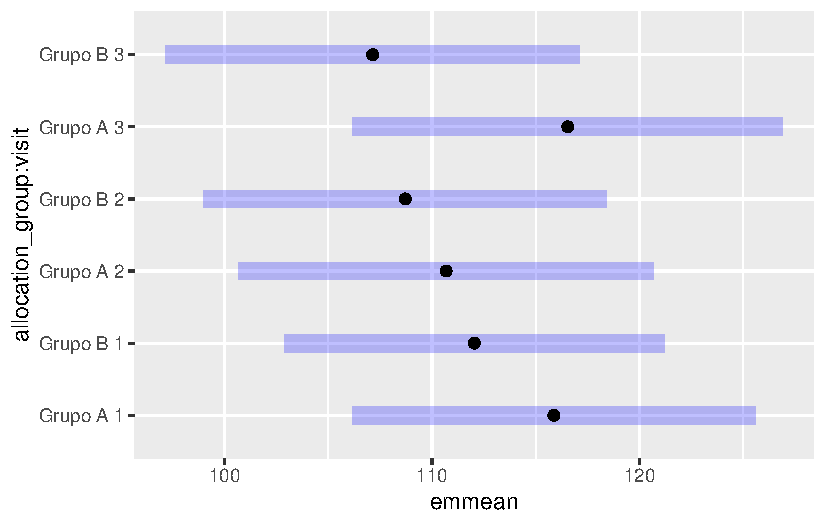
\includegraphics{Outcomes_files/figure-pdf/labs_ldl_sens_emm-1.pdf}

\paragraph{Resultado}\label{resultado-5}

No modelo ajustado para os níveis de LDL-colesterol, não foram
observadas diferenças estatisticamente significativas entre os grupos em
nenhum dos três momentos avaliados. Da mesma forma, as comparações
dentro de cada grupo ao longo do tempo não indicaram alterações
significativas. A análise de sensibilidade, com exclusão das observações
influentes, não modificou substancialmente os achados: as estimativas
permaneceram estáveis e todas as comparações continuaram não
significativas. As estimativas, intervalos de confiança de 95\% e
valores de p estão apresentados na Tabela~\ref{tbl-ldl}.

\begin{longtable}[]{@{}
  >{\raggedright\arraybackslash}p{(\columnwidth - 8\tabcolsep) * \real{0.2000}}
  >{\raggedright\arraybackslash}p{(\columnwidth - 8\tabcolsep) * \real{0.2000}}
  >{\raggedright\arraybackslash}p{(\columnwidth - 8\tabcolsep) * \real{0.2000}}
  >{\raggedright\arraybackslash}p{(\columnwidth - 8\tabcolsep) * \real{0.2000}}
  >{\raggedright\arraybackslash}p{(\columnwidth - 8\tabcolsep) * \real{0.2000}}@{}}
\caption{Diferenças estimadas dos níveis de LDL-colesterol entre os
grupos de alocação (placebo vs Eclipta) e entre visitas dentro de cada
grupo}\label{tbl-ldl}\tabularnewline
\toprule\noalign{}
\begin{minipage}[b]{\linewidth}\raggedright
Grupo de comparação
\end{minipage} & \begin{minipage}[b]{\linewidth}\raggedright
Comparação
\end{minipage} & \begin{minipage}[b]{\linewidth}\raggedright
Estimativa
\end{minipage} & \begin{minipage}[b]{\linewidth}\raggedright
IC 95\%
\end{minipage} & \begin{minipage}[b]{\linewidth}\raggedright
p-valor
\end{minipage} \\
\midrule\noalign{}
\endfirsthead
\toprule\noalign{}
\begin{minipage}[b]{\linewidth}\raggedright
Grupo de comparação
\end{minipage} & \begin{minipage}[b]{\linewidth}\raggedright
Comparação
\end{minipage} & \begin{minipage}[b]{\linewidth}\raggedright
Estimativa
\end{minipage} & \begin{minipage}[b]{\linewidth}\raggedright
IC 95\%
\end{minipage} & \begin{minipage}[b]{\linewidth}\raggedright
p-valor
\end{minipage} \\
\midrule\noalign{}
\endhead
\bottomrule\noalign{}
\endlastfoot
Entre grupos & Visita 1 & 3,77 & {[}-9,63 ; 17,17{]} & 0,578 \\
Entre grupos & Visita 2 & 1,85 & {[}-12,56 ; 16,26{]} & 0,799 \\
Entre grupos & Visita 3 & 9,68 & {[}-5,41 ; 24,78{]} & 0,207 \\
Grupo Placebo & Visita 1 - Visita 2 & 5,59 & {[}-4,07 ; 15,26{]} &
0,486 \\
Grupo Placebo & Visita 1 - Visita 3 & 0,02 & {[}-10,46 ; 10,50{]} &
1,000 \\
Grupo Placebo & Visita 2 - Visita 3 & -5,57 & {[}-16,13 ; 4,98{]} &
0,606 \\
Grupo Eclipta & Visita 1 - Visita 2 & 3,67 & {[}-6,71 ; 14,06{]} &
1,000 \\
Grupo Eclipta & Visita 1 - Visita 3 & 5,93 & {[}-5,15 ; 17,00{]} &
0,586 \\
Grupo Eclipta & Visita 2 - Visita 3 & 2,25 & {[}-9,26 ; 13,76{]} &
1,000 \\
\end{longtable}

\begin{Shaded}
\begin{Highlighting}[]
\FunctionTok{ggplot}\NormalTok{(}
    \AttributeTok{data =}\NormalTok{ data\_model, }
    \FunctionTok{aes}\NormalTok{(}
        \AttributeTok{x =} \FunctionTok{as.factor}\NormalTok{(visit),}
        \AttributeTok{y =}\NormalTok{ labs\_ldl,}
        \AttributeTok{group =}\NormalTok{ record\_id,}
\NormalTok{    )}
\NormalTok{) }\SpecialCharTok{+}
    \FunctionTok{geom\_line}\NormalTok{(}\AttributeTok{alpha =} \FloatTok{0.5}\NormalTok{) }\SpecialCharTok{+}
    \FunctionTok{geom\_point}\NormalTok{(}\AttributeTok{alpha =} \FloatTok{0.7}\NormalTok{) }\SpecialCharTok{+}
    \FunctionTok{geom\_smooth}\NormalTok{(}
        \FunctionTok{aes}\NormalTok{(}\AttributeTok{group =}\NormalTok{ allocation\_group),}
        \AttributeTok{method =} \StringTok{"lm"}\NormalTok{,}
        \AttributeTok{se =} \ConstantTok{TRUE}\NormalTok{,}
        \AttributeTok{linewidth =} \DecValTok{1}
\NormalTok{    ) }\SpecialCharTok{+}
    \FunctionTok{labs}\NormalTok{(}\AttributeTok{title =} \StringTok{"All data"}\NormalTok{) }\SpecialCharTok{+}
    \FunctionTok{facet\_wrap}\NormalTok{(}\SpecialCharTok{\textasciitilde{}}\NormalTok{ allocation\_group) }
\end{Highlighting}
\end{Shaded}

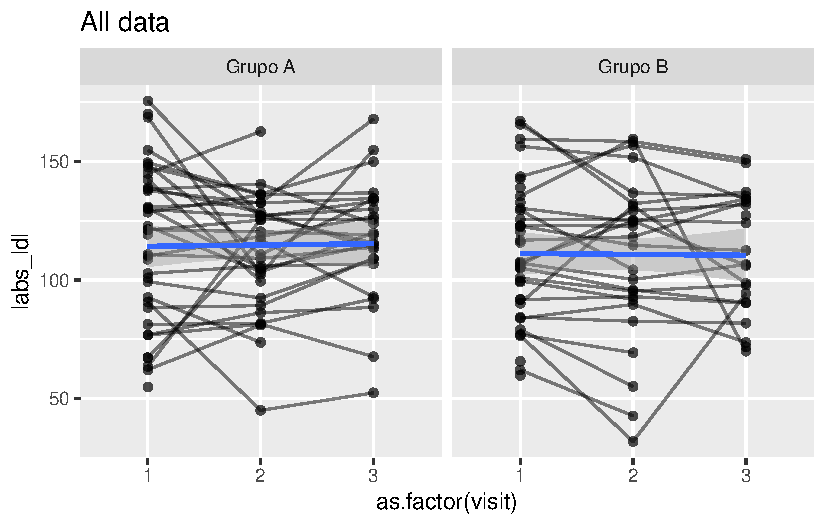
\includegraphics{Outcomes_files/figure-pdf/labs_ldl_6-1.pdf}

\begin{Shaded}
\begin{Highlighting}[]
    \CommentTok{\#coord\_cartesian(ylim = c(10, 150))}

\NormalTok{data\_model }\SpecialCharTok{\%\textgreater{}\%} 
    \FunctionTok{filter}\NormalTok{(}
        \SpecialCharTok{!}\NormalTok{(record\_id }\SpecialCharTok{\%in\%} 
\NormalTok{        labs\_ldl\_model\_check}\SpecialCharTok{$}\NormalTok{influential\_ids)}
\NormalTok{    ) }\SpecialCharTok{\%\textgreater{}\%} 
    \FunctionTok{ggplot}\NormalTok{(}
        \FunctionTok{aes}\NormalTok{(}
            \AttributeTok{x =} \FunctionTok{as.factor}\NormalTok{(visit),}
            \AttributeTok{y =}\NormalTok{ labs\_ldl,}
            \AttributeTok{group =}\NormalTok{ record\_id,}
\NormalTok{        )}
\NormalTok{    ) }\SpecialCharTok{+}
    \FunctionTok{geom\_line}\NormalTok{(}\AttributeTok{alpha =} \FloatTok{0.5}\NormalTok{) }\SpecialCharTok{+}
    \FunctionTok{geom\_point}\NormalTok{(}\AttributeTok{alpha =} \FloatTok{0.7}\NormalTok{) }\SpecialCharTok{+}
    \FunctionTok{geom\_smooth}\NormalTok{(}
        \FunctionTok{aes}\NormalTok{(}\AttributeTok{group =}\NormalTok{ allocation\_group),}
        \AttributeTok{method =} \StringTok{"lm"}\NormalTok{,}
        \AttributeTok{se =} \ConstantTok{TRUE}\NormalTok{,}
        \AttributeTok{linewidth =} \DecValTok{1}
\NormalTok{    ) }\SpecialCharTok{+}
    \FunctionTok{labs}\NormalTok{(}\AttributeTok{title =} \StringTok{"Sensitivity analysis"}\NormalTok{) }\SpecialCharTok{+}
    \FunctionTok{facet\_wrap}\NormalTok{(}\SpecialCharTok{\textasciitilde{}}\NormalTok{ allocation\_group) }
\end{Highlighting}
\end{Shaded}

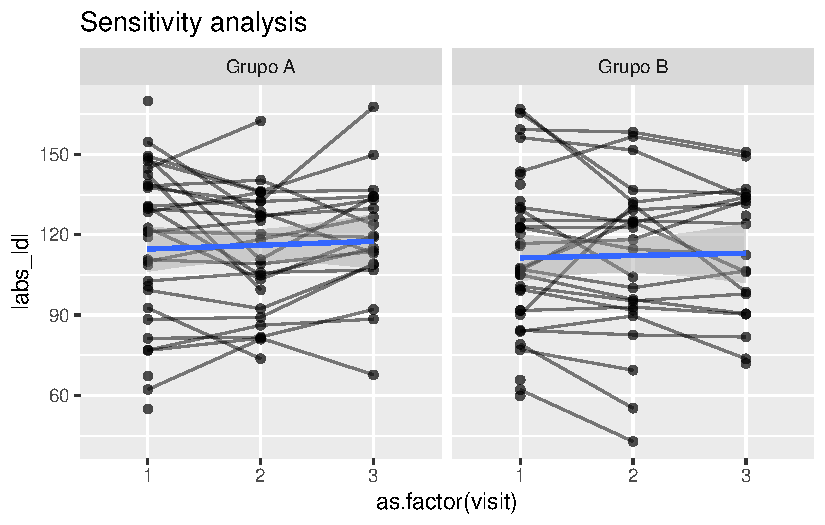
\includegraphics{Outcomes_files/figure-pdf/labs_ldl_6-2.pdf}

\begin{Shaded}
\begin{Highlighting}[]
    \CommentTok{\#coord\_cartesian(ylim = c(10, 150))}
\end{Highlighting}
\end{Shaded}

\subsubsection{HDL Colesterol}\label{hdl-colesterol}

Variável: \texttt{labs\_hdl}

\begin{Shaded}
\begin{Highlighting}[]
\CommentTok{\# Plot 1: Raw data}
\NormalTok{labs\_hdl\_hist\_1 }\OtherTok{\textless{}{-}}\NormalTok{ data\_model }\SpecialCharTok{\%\textgreater{}\%} 
    \CommentTok{\#filter(}
    \CommentTok{\#    labs\_hdl \textless{} 300}
    \CommentTok{\#) \%\textgreater{}\% }
    \FunctionTok{ggplot}\NormalTok{(}\FunctionTok{aes}\NormalTok{(}\AttributeTok{x =}\NormalTok{ labs\_hdl)) }\SpecialCharTok{+} 
    \FunctionTok{geom\_histogram}\NormalTok{(}\AttributeTok{bins =} \DecValTok{50}\NormalTok{, }\AttributeTok{fill =} \StringTok{"skyblue"}\NormalTok{, }\AttributeTok{color =} \StringTok{"black"}\NormalTok{)}

\CommentTok{\# Plot 2: Log{-}transformed data}
\NormalTok{labs\_hdl\_hist\_2 }\OtherTok{\textless{}{-}}\NormalTok{ data\_model }\SpecialCharTok{\%\textgreater{}\%} 
    \CommentTok{\#filter(}
    \CommentTok{\#    labs\_hdl \textless{} 300}
    \CommentTok{\#) \%\textgreater{}\%}
    \FunctionTok{ggplot}\NormalTok{(}\FunctionTok{aes}\NormalTok{(}\AttributeTok{x =} \FunctionTok{log1p}\NormalTok{(labs\_hdl))) }\SpecialCharTok{+} 
    \FunctionTok{geom\_histogram}\NormalTok{(}\AttributeTok{bins =} \DecValTok{50}\NormalTok{, }\AttributeTok{fill =} \StringTok{"lightgreen"}\NormalTok{, }\AttributeTok{color =} \StringTok{"black"}\NormalTok{)}

\CommentTok{\# Combine side by side}
\NormalTok{labs\_hdl\_hist\_1 }\SpecialCharTok{+}\NormalTok{ labs\_hdl\_hist\_2 }\CommentTok{\# library(patchwork)}
\end{Highlighting}
\end{Shaded}

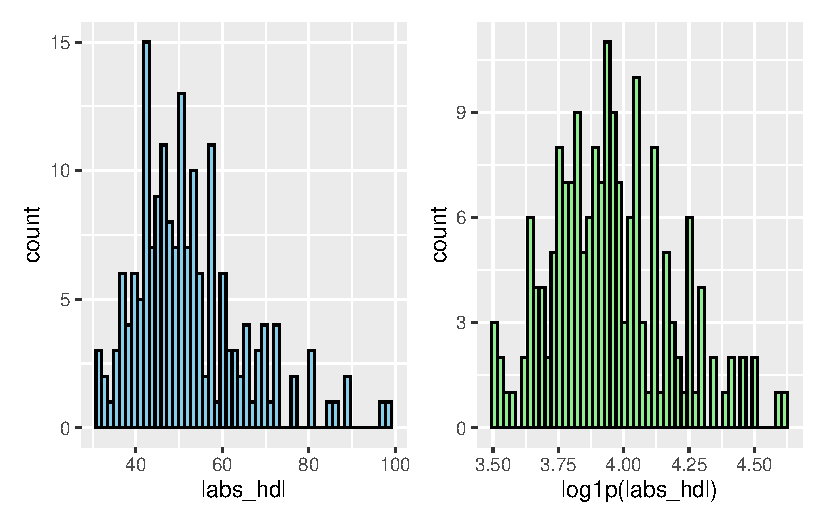
\includegraphics{Outcomes_files/figure-pdf/labs_hdl_1-1.pdf}

\begin{Shaded}
\begin{Highlighting}[]
\CommentTok{\# LMM}
\NormalTok{labs\_hdl\_model }\OtherTok{\textless{}{-}} \FunctionTok{lmer}\NormalTok{(}\FunctionTok{log1p}\NormalTok{(labs\_hdl) }\SpecialCharTok{\textasciitilde{}}\NormalTok{ allocation\_group }\SpecialCharTok{*}\NormalTok{ visit }\SpecialCharTok{+} 
\NormalTok{(}\DecValTok{1} \SpecialCharTok{|}\NormalTok{ record\_id), }\AttributeTok{data =}\NormalTok{ data\_model)}
\FunctionTok{check\_collinearity}\NormalTok{(labs\_hdl\_model)}
\end{Highlighting}
\end{Shaded}

\begin{verbatim}
# Check for Multicollinearity

Low Correlation

                   Term  VIF   VIF 95% CI Increased SE Tolerance Tolerance 95% CI
       allocation_group 1.16 [1.05, 1.51]         1.08      0.86     [0.66, 0.95]
                  visit 3.49 [2.78, 4.48]         1.87      0.29     [0.22, 0.36]
 allocation_group:visit 3.74 [2.97, 4.81]         1.93      0.27     [0.21, 0.34]
\end{verbatim}

\begin{Shaded}
\begin{Highlighting}[]
\CommentTok{\# Sensitivity analysis}
\NormalTok{labs\_hdl\_model\_check }\OtherTok{\textless{}{-}} \FunctionTok{sensitivity\_check\_lmer}\NormalTok{(}
    \AttributeTok{model =}\NormalTok{ labs\_hdl\_model,}
    \AttributeTok{id\_var =} \StringTok{"record\_id"}\NormalTok{,}
    \AttributeTok{top\_n =} \DecValTok{5}\NormalTok{)}

\CommentTok{\# LMM Sensitivity}
\NormalTok{labs\_hdl\_model\_sens }\OtherTok{\textless{}{-}} \FunctionTok{update}\NormalTok{(}\AttributeTok{object =}\NormalTok{ labs\_hdl\_model,}
                              \AttributeTok{subset =} \SpecialCharTok{!}\NormalTok{(record\_id }\SpecialCharTok{\%in\%} 
\NormalTok{        labs\_hdl\_model\_check}\SpecialCharTok{$}\NormalTok{influential\_ids))}
\CommentTok{\# Influential IDS}
\NormalTok{labs\_hdl\_model\_check}\SpecialCharTok{$}\NormalTok{influential\_ids}
\end{Highlighting}
\end{Shaded}

\begin{verbatim}
[1] "16" "75" "38" "42" "26"
\end{verbatim}

\paragraph{Resumo dos modelos}\label{resumo-dos-modelos-6}

\begin{Shaded}
\begin{Highlighting}[]
\CommentTok{\# Model comparison}
\FunctionTok{summary}\NormalTok{(labs\_hdl\_model)}
\end{Highlighting}
\end{Shaded}

\begin{verbatim}
Linear mixed model fit by REML. t-tests use Satterthwaite's method ['lmerModLmerTest']
Formula: log1p(labs_hdl) ~ allocation_group * visit + (1 | record_id)
   Data: data_model

REML criterion at convergence: -79.8

Scaled residuals: 
    Min      1Q  Median      3Q     Max 
-2.4161 -0.4907 -0.0289  0.4389  3.0395 

Random effects:
 Groups    Name        Variance Std.Dev.
 record_id (Intercept) 0.03949  0.1987  
 Residual              0.01437  0.1199  
Number of obs: 179, groups:  record_id, 75

Fixed effects:
                                Estimate Std. Error        df t value Pr(>|t|)    
(Intercept)                      3.94481    0.03815  94.81644 103.399   <2e-16 ***
allocation_groupGrupo B          0.06500    0.05360  94.81644   1.213    0.228    
visit2                          -0.01725    0.03011 102.74671  -0.573    0.568    
visit3                          -0.01928    0.03264 103.82312  -0.591    0.556    
allocation_groupGrupo B:visit2  -0.02214    0.04420 104.26672  -0.501    0.618    
allocation_groupGrupo B:visit3  -0.03185    0.04749 105.05887  -0.671    0.504    
---
Signif. codes:  0 '***' 0.001 '**' 0.01 '*' 0.05 '.' 0.1 ' ' 1

Correlation of Fixed Effects:
            (Intr) all_GB visit2 visit3 a_GB:2
allctn_grGB -0.712                            
visit2      -0.338  0.241                     
visit3      -0.312  0.222  0.451              
allctn_GB:2  0.230 -0.324 -0.681 -0.307       
allctn_GB:3  0.214 -0.301 -0.310 -0.687  0.435
\end{verbatim}

\begin{Shaded}
\begin{Highlighting}[]
\FunctionTok{summary}\NormalTok{(labs\_hdl\_model\_sens)}
\end{Highlighting}
\end{Shaded}

\begin{verbatim}
Linear mixed model fit by REML. t-tests use Satterthwaite's method ['lmerModLmerTest']
Formula: log1p(labs_hdl) ~ allocation_group * visit + (1 | record_id)
   Data: data_model
 Subset: !(record_id %in% labs_hdl_model_check$influential_ids)

REML criterion at convergence: -109.5

Scaled residuals: 
     Min       1Q   Median       3Q      Max 
-1.93721 -0.52772 -0.00876  0.50466  2.04629 

Random effects:
 Groups    Name        Variance Std.Dev.
 record_id (Intercept) 0.03870  0.1967  
 Residual              0.01007  0.1004  
Number of obs: 166, groups:  record_id, 70

Fixed effects:
                               Estimate Std. Error       df t value Pr(>|t|)    
(Intercept)                     3.92823    0.03733 82.44138 105.230   <2e-16 ***
allocation_groupGrupo B         0.06708    0.05279 82.44138   1.271    0.207    
visit2                         -0.01029    0.02612 93.87428  -0.394    0.695    
visit3                         -0.01338    0.02805 94.47459  -0.477    0.635    
allocation_groupGrupo B:visit2 -0.02943    0.03859 95.06373  -0.763    0.448    
allocation_groupGrupo B:visit3 -0.03861    0.04187 95.58326  -0.922    0.359    
---
Signif. codes:  0 '***' 0.001 '**' 0.01 '*' 0.05 '.' 0.1 ' ' 1

Correlation of Fixed Effects:
            (Intr) all_GB visit2 visit3 a_GB:2
allctn_grGB -0.707                            
visit2      -0.295  0.209                     
visit3      -0.275  0.194  0.457              
allctn_GB:2  0.200 -0.283 -0.677 -0.310       
allctn_GB:3  0.184 -0.260 -0.306 -0.670  0.440
\end{verbatim}

\begin{Shaded}
\begin{Highlighting}[]
\NormalTok{labs\_hdl\_model\_check}\SpecialCharTok{$}\NormalTok{comparison\_table}
\end{Highlighting}
\end{Shaded}

\begin{verbatim}
# A tibble: 16 x 6
   Model       term                           estimate std.error statistic   p.value
   <chr>       <chr>                             <dbl>     <dbl>     <dbl>     <dbl>
 1 Original    (Intercept)                      3.94      0.0382   103.     2.78e-99
 2 Sensitivity (Intercept)                      3.93      0.0373   105.     1.23e-89
 3 Original    allocation_groupGrupo B          0.0650    0.0536     1.21   2.28e- 1
 4 Sensitivity allocation_groupGrupo B          0.0671    0.0528     1.27   2.07e- 1
 5 Original    allocation_groupGrupo B:visit2  -0.0221    0.0442    -0.501  6.18e- 1
 6 Sensitivity allocation_groupGrupo B:visit2  -0.0294    0.0386    -0.763  4.48e- 1
 7 Original    allocation_groupGrupo B:visit3  -0.0318    0.0475    -0.671  5.04e- 1
 8 Sensitivity allocation_groupGrupo B:visit3  -0.0386    0.0419    -0.922  3.59e- 1
 9 Original    sd__(Intercept)                  0.199    NA         NA     NA       
10 Sensitivity sd__(Intercept)                  0.197    NA         NA     NA       
11 Original    sd__Observation                  0.120    NA         NA     NA       
12 Sensitivity sd__Observation                  0.100    NA         NA     NA       
13 Original    visit2                          -0.0172    0.0301    -0.573  5.68e- 1
14 Sensitivity visit2                          -0.0103    0.0261    -0.394  6.95e- 1
15 Original    visit3                          -0.0193    0.0326    -0.591  5.56e- 1
16 Sensitivity visit3                          -0.0134    0.0281    -0.477  6.35e- 1
\end{verbatim}

\begin{Shaded}
\begin{Highlighting}[]
\NormalTok{performance}\SpecialCharTok{::}\FunctionTok{compare\_performance}\NormalTok{(}
\NormalTok{    labs\_hdl\_model, }
\NormalTok{    labs\_hdl\_model\_sens) }
\end{Highlighting}
\end{Shaded}

\begin{verbatim}
# Comparison of Model Performance Indices

Name                |           Model |  AIC (weights) | AICc (weights) |  BIC (weights) | R2 (cond.) | R2 (marg.) |   ICC |  RMSE | Sigma
------------------------------------------------------------------------------------------------------------------------------------------
labs_hdl_model      | lmerModLmerTest | 1319.8 (<.001) | 1320.7 (<.001) | 1345.3 (<.001) |      0.738 |      0.017 | 0.733 | 0.094 | 0.120
labs_hdl_model_sens | lmerModLmerTest | 1181.6 (>.999) | 1182.5 (>.999) | 1206.5 (>.999) |      0.797 |      0.018 | 0.793 | 0.078 | 0.100
\end{verbatim}

\begin{Shaded}
\begin{Highlighting}[]
\NormalTok{performance}\SpecialCharTok{::}\FunctionTok{check\_model}\NormalTok{(labs\_hdl\_model)}
\end{Highlighting}
\end{Shaded}

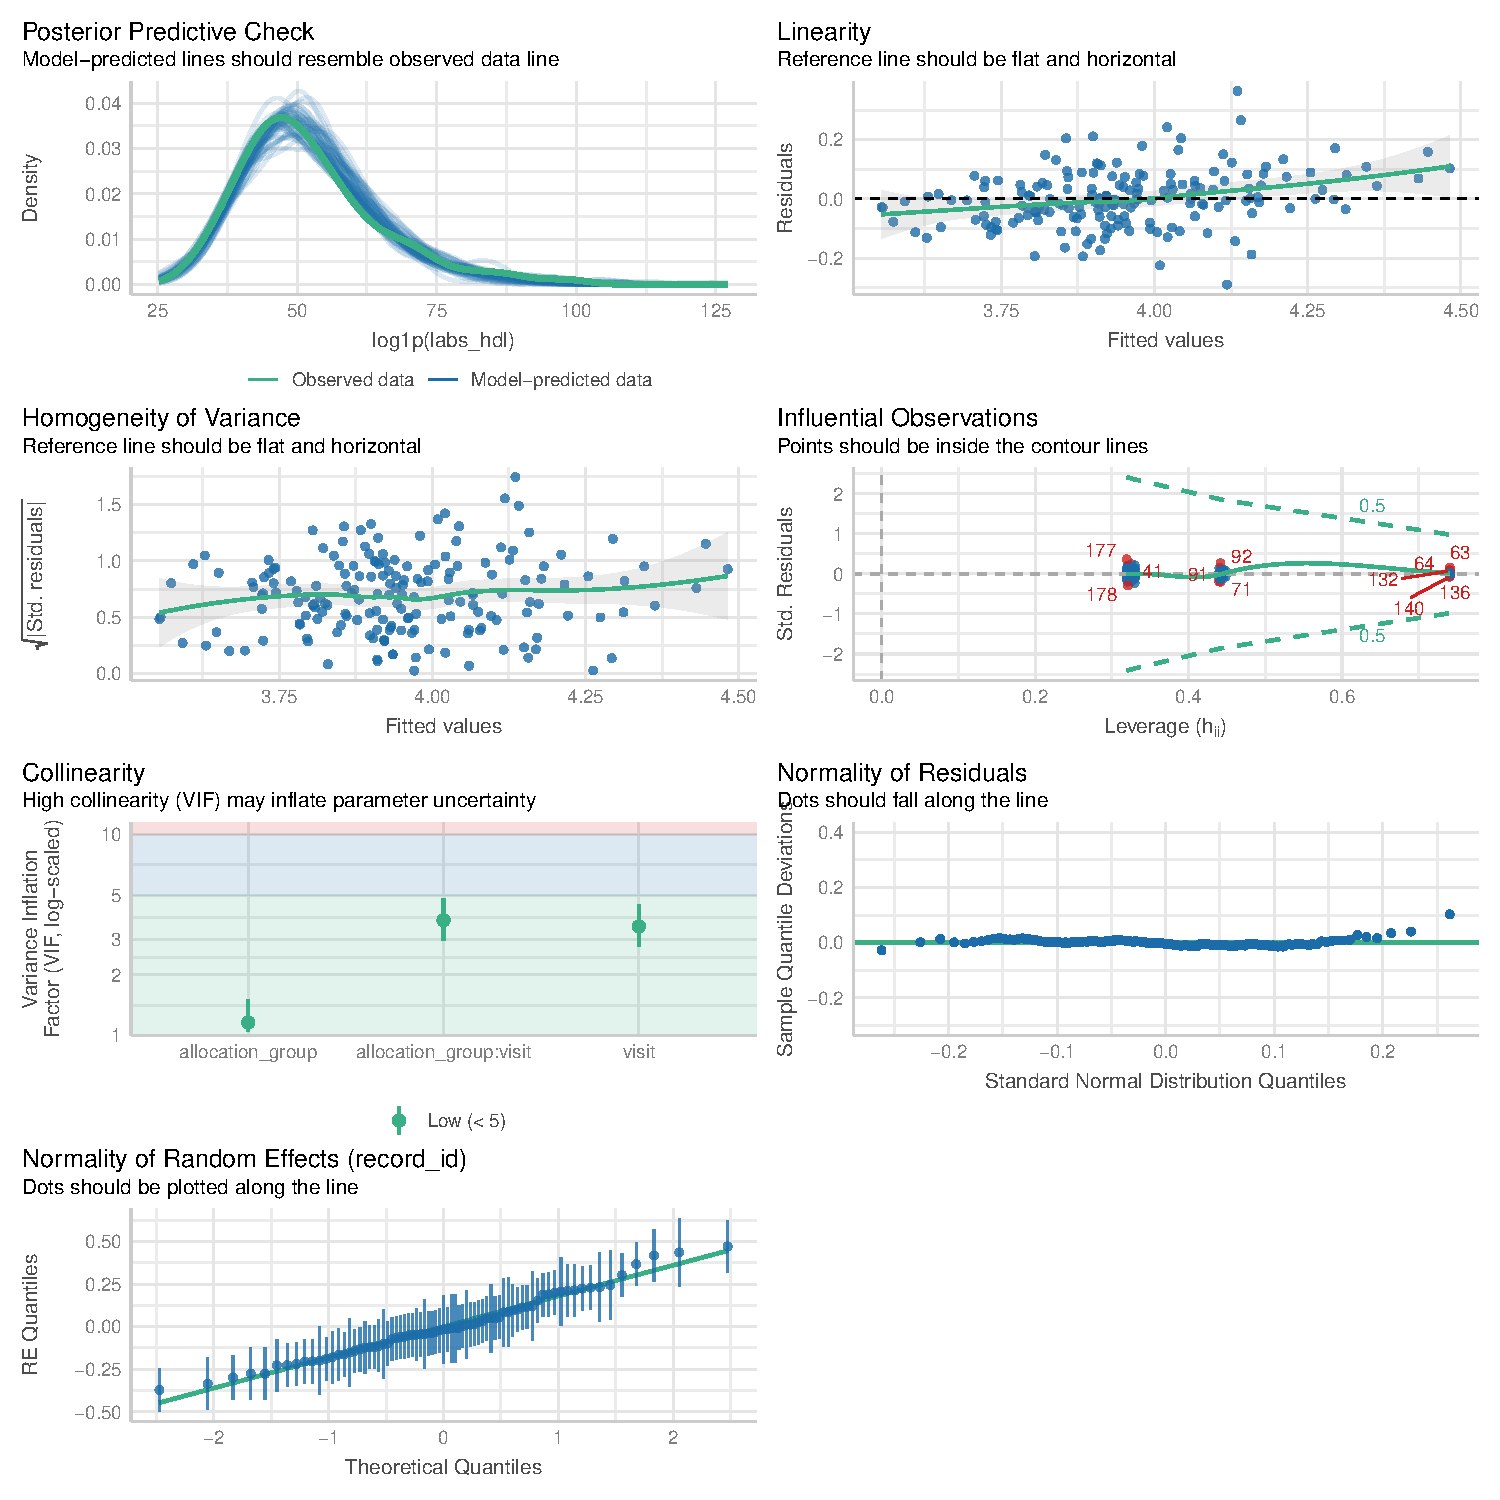
\includegraphics{Outcomes_files/figure-pdf/labs_hdl_4-1.pdf}

\begin{Shaded}
\begin{Highlighting}[]
\NormalTok{performance}\SpecialCharTok{::}\FunctionTok{check\_model}\NormalTok{(labs\_hdl\_model\_sens)}
\end{Highlighting}
\end{Shaded}

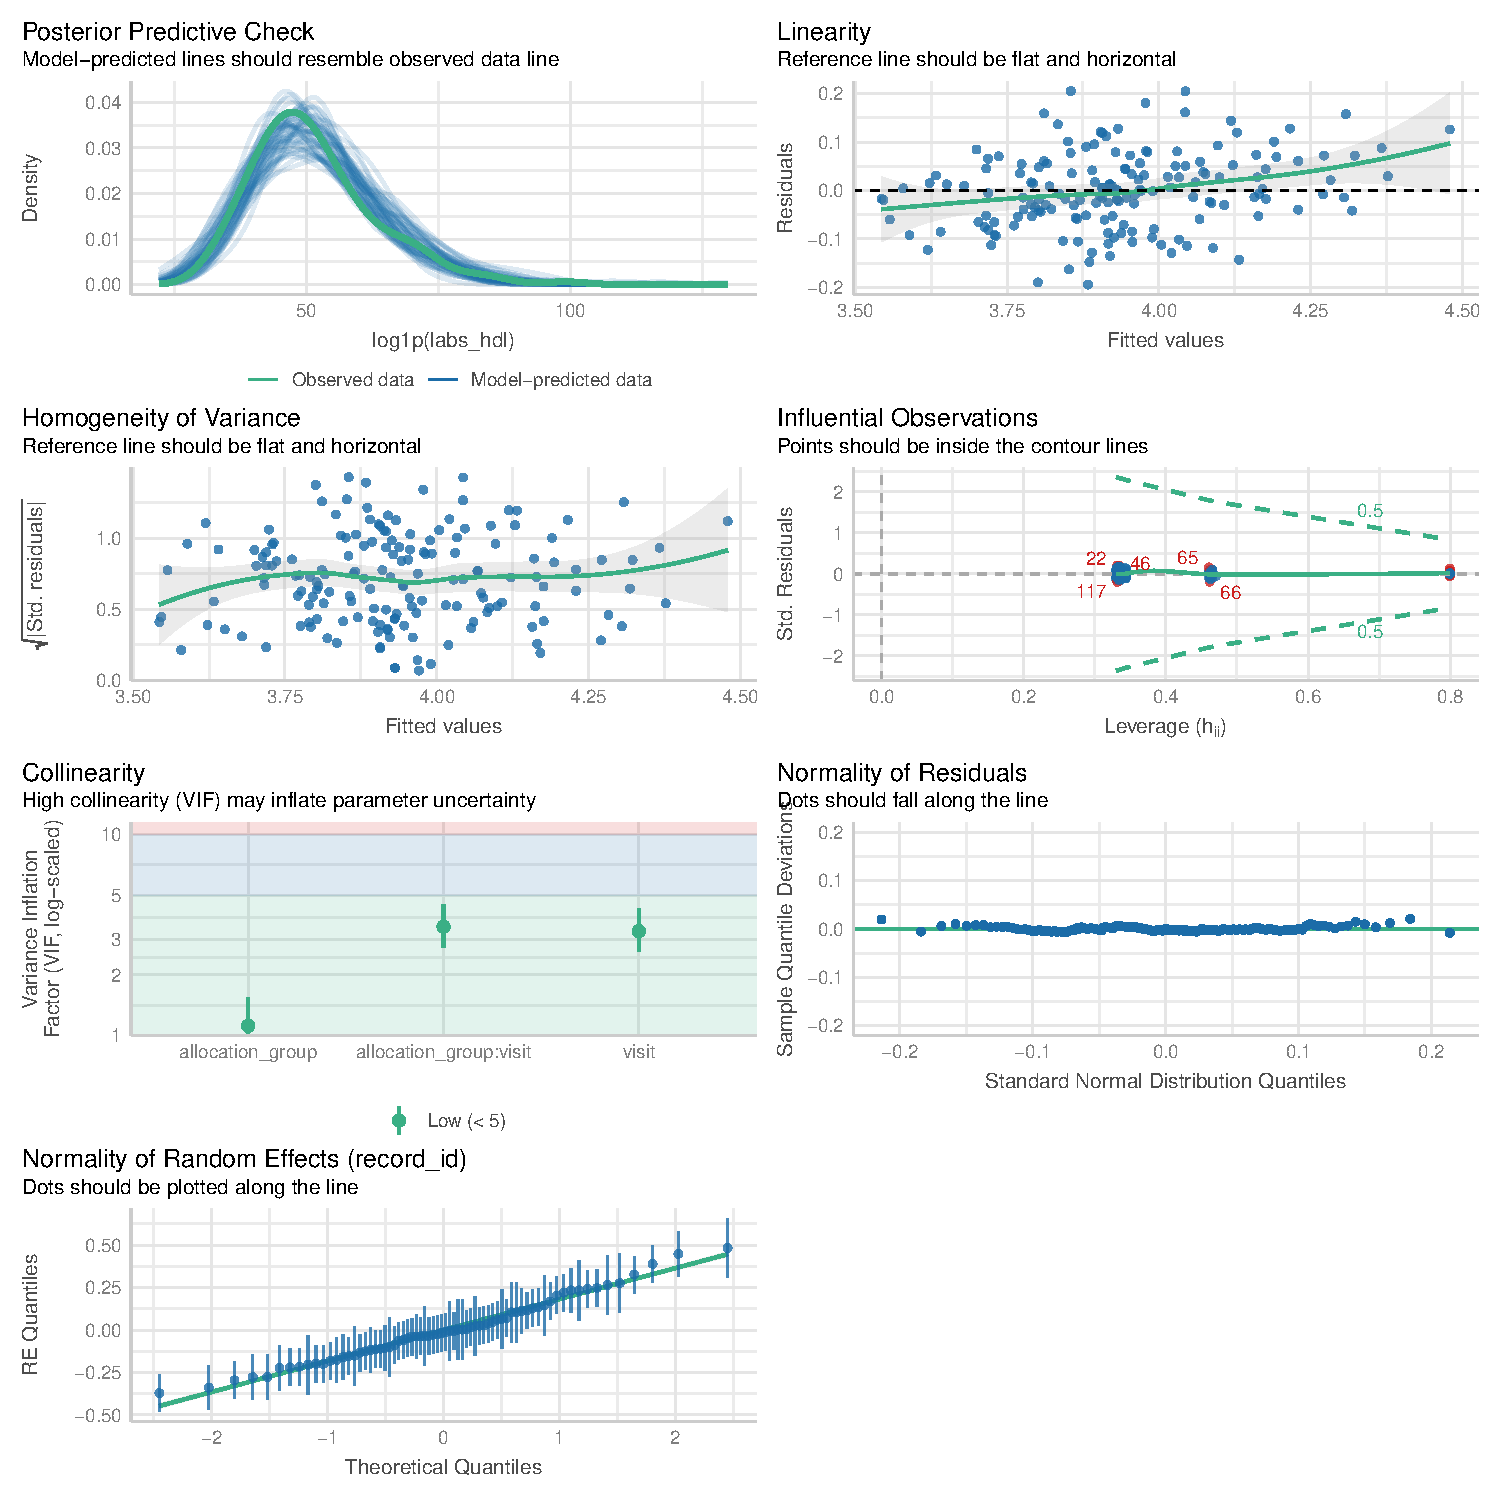
\includegraphics{Outcomes_files/figure-pdf/labs_hdl_4-2.pdf}

\paragraph{Médias Marginais
Estimadas}\label{muxe9dias-marginais-estimadas-6}

\subparagraph{Todos os dados}\label{todos-os-dados-6}

\begin{Shaded}
\begin{Highlighting}[]
\CommentTok{\# Get EMMs for each group at each visit}
\NormalTok{labs\_hdl\_raw\_emm }\OtherTok{\textless{}{-}}\NormalTok{ emmeans}\SpecialCharTok{::}\FunctionTok{emmeans}\NormalTok{(}
\NormalTok{    labs\_hdl\_model, }
    \SpecialCharTok{\textasciitilde{}}\NormalTok{ allocation\_group }\SpecialCharTok{*}\NormalTok{ visit}
\NormalTok{)}

\NormalTok{labs\_hdl\_raw\_emm }\OtherTok{\textless{}{-}} \FunctionTok{regrid}\NormalTok{(labs\_hdl\_raw\_emm)}

\CommentTok{\# Table of marginal means}
\CommentTok{\# labs\_hdl\_raw\_emm}

\CommentTok{\# Pairwise comparisons: Between groups at each visit}
\NormalTok{emmeans}\SpecialCharTok{::}\FunctionTok{contrast}\NormalTok{(labs\_hdl\_raw\_emm,}
\AttributeTok{method =} \StringTok{"pairwise"}\NormalTok{, }\AttributeTok{by =} \StringTok{"visit"}\NormalTok{,}
\AttributeTok{adjust =} \StringTok{"bonferroni"}\NormalTok{) }\SpecialCharTok{\%\textgreater{}\%} \FunctionTok{summary}\NormalTok{(}\AttributeTok{infer =} \FunctionTok{c}\NormalTok{(}\ConstantTok{TRUE}\NormalTok{, }\ConstantTok{TRUE}\NormalTok{))}
\end{Highlighting}
\end{Shaded}

\begin{verbatim}
visit = 1:
 contrast          estimate   SE    df lower.CL upper.CL t.ratio p.value
 Grupo A - Grupo B    -3.47 2.86  96.4    -9.15     2.21  -1.212  0.2284

visit = 2:
 contrast          estimate   SE    df lower.CL upper.CL t.ratio p.value
 Grupo A - Grupo B    -2.22 2.98 108.6    -8.14     3.69  -0.746  0.4576

visit = 3:
 contrast          estimate   SE    df lower.CL upper.CL t.ratio p.value
 Grupo A - Grupo B    -1.71 3.09 123.5    -7.83     4.42  -0.552  0.5819

Degrees-of-freedom method: inherited from kenward-roger when re-gridding 
Confidence level used: 0.95 
\end{verbatim}

\begin{Shaded}
\begin{Highlighting}[]
\CommentTok{\# Pairwise comparisons: Changes over time within each group}
\NormalTok{emmeans}\SpecialCharTok{::}\FunctionTok{contrast}\NormalTok{(labs\_hdl\_raw\_emm,}
\AttributeTok{method =} \StringTok{"pairwise"}\NormalTok{, }\AttributeTok{by =} \StringTok{"allocation\_group"}\NormalTok{,}
\AttributeTok{adjust =} \StringTok{"bonferroni"}\NormalTok{) }\SpecialCharTok{\%\textgreater{}\%} \FunctionTok{summary}\NormalTok{(}\AttributeTok{infer =} \FunctionTok{c}\NormalTok{(}\ConstantTok{TRUE}\NormalTok{, }\ConstantTok{TRUE}\NormalTok{))}
\end{Highlighting}
\end{Shaded}

\begin{verbatim}
allocation_group = Grupo A:
 contrast        estimate   SE    df lower.CL upper.CL t.ratio p.value
 visit1 - visit2    0.883 1.54  96.4    -2.87     4.64   0.573  1.0000
 visit1 - visit3    0.986 1.67  96.4    -3.08     5.05   0.591  1.0000
 visit2 - visit3    0.103 1.67 108.6    -3.96     4.17   0.062  1.0000

allocation_group = Grupo B:
 contrast        estimate   SE    df lower.CL upper.CL t.ratio p.value
 visit1 - visit2    2.129 1.74  96.4    -2.12     6.38   1.221  0.6751
 visit1 - visit3    2.748 1.84  96.4    -1.74     7.24   1.491  0.4175
 visit2 - visit3    0.619 1.90 123.2    -3.99     5.22   0.326  1.0000

Degrees-of-freedom method: inherited from kenward-roger when re-gridding 
Confidence level used: 0.95 
Conf-level adjustment: bonferroni method for 3 estimates 
P value adjustment: bonferroni method for 3 tests 
\end{verbatim}

\begin{Shaded}
\begin{Highlighting}[]
\CommentTok{\# Plot of marginal means}
\FunctionTok{plot}\NormalTok{(labs\_hdl\_raw\_emm, }\AttributeTok{comparisons =} \ConstantTok{TRUE}\NormalTok{)}
\end{Highlighting}
\end{Shaded}

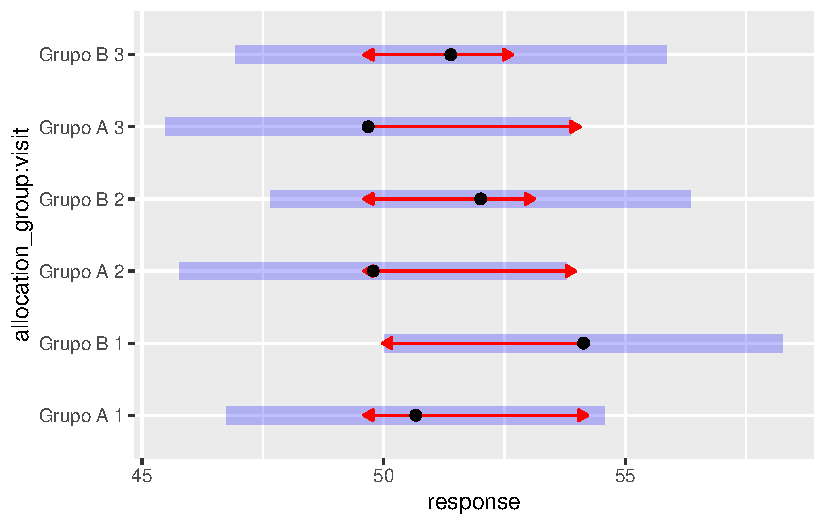
\includegraphics{Outcomes_files/figure-pdf/labs_hdl_raw_emm-1.pdf}

\subparagraph{Análise de
sensibilidade}\label{anuxe1lise-de-sensibilidade-6}

\begin{Shaded}
\begin{Highlighting}[]
\CommentTok{\# Get EMMs for each group at each visit (Sensitivity Analysis)}
\NormalTok{labs\_hdl\_emm }\OtherTok{\textless{}{-}}\NormalTok{ emmeans}\SpecialCharTok{::}\FunctionTok{emmeans}\NormalTok{(}
\NormalTok{    labs\_hdl\_model\_sens, }
    \SpecialCharTok{\textasciitilde{}}\NormalTok{ allocation\_group }\SpecialCharTok{*}\NormalTok{ visit}
\NormalTok{)}

\NormalTok{labs\_hdl\_emm }\OtherTok{\textless{}{-}} \FunctionTok{regrid}\NormalTok{(labs\_hdl\_emm)}

\CommentTok{\# Table of marginal means}
\CommentTok{\# labs\_hdl\_emm}

\CommentTok{\# Pairwise comparisons: Between groups at each visit}
\NormalTok{emmeans}\SpecialCharTok{::}\FunctionTok{contrast}\NormalTok{(labs\_hdl\_emm,}
\AttributeTok{method =} \StringTok{"pairwise"}\NormalTok{, }\AttributeTok{by =} \StringTok{"visit"}\NormalTok{,}
\AttributeTok{adjust =} \StringTok{"bonferroni"}\NormalTok{) }\SpecialCharTok{\%\textgreater{}\%} \FunctionTok{summary}\NormalTok{(}\AttributeTok{infer =} \FunctionTok{c}\NormalTok{(}\ConstantTok{TRUE}\NormalTok{, }\ConstantTok{TRUE}\NormalTok{))}
\end{Highlighting}
\end{Shaded}

\begin{verbatim}
visit = 1:
 contrast          estimate   SE    df lower.CL upper.CL t.ratio p.value
 Grupo A - Grupo B    -3.53 2.78  83.9    -9.05     2.00  -1.269  0.2078

visit = 2:
 contrast          estimate   SE    df lower.CL upper.CL t.ratio p.value
 Grupo A - Grupo B    -1.93 2.87  93.9    -7.63     3.77  -0.672  0.5029

visit = 3:
 contrast          estimate   SE    df lower.CL upper.CL t.ratio p.value
 Grupo A - Grupo B    -1.45 2.97 104.0    -7.33     4.43  -0.488  0.6264

Degrees-of-freedom method: inherited from kenward-roger when re-gridding 
Confidence level used: 0.95 
\end{verbatim}

\begin{Shaded}
\begin{Highlighting}[]
\CommentTok{\# Pairwise comparisons: Changes over time within each group}
\NormalTok{emmeans}\SpecialCharTok{::}\FunctionTok{contrast}\NormalTok{(labs\_hdl\_emm,}
\AttributeTok{method =} \StringTok{"pairwise"}\NormalTok{, }\AttributeTok{by =} \StringTok{"allocation\_group"}\NormalTok{,}
\AttributeTok{adjust =} \StringTok{"bonferroni"}\NormalTok{) }\SpecialCharTok{\%\textgreater{}\%} \FunctionTok{summary}\NormalTok{(}\AttributeTok{infer =} \FunctionTok{c}\NormalTok{(}\ConstantTok{TRUE}\NormalTok{, }\ConstantTok{TRUE}\NormalTok{))}
\end{Highlighting}
\end{Shaded}

\begin{verbatim}
allocation_group = Grupo A:
 contrast        estimate   SE    df lower.CL upper.CL t.ratio p.value
 visit1 - visit2    0.520 1.32  83.9    -2.71     3.75   0.394  1.0000
 visit1 - visit3    0.675 1.41  83.9    -2.78     4.13   0.477  1.0000
 visit2 - visit3    0.155 1.42  93.9    -3.31     3.62   0.109  1.0000

allocation_group = Grupo B:
 contrast        estimate   SE    df lower.CL upper.CL t.ratio p.value
 visit1 - visit2    2.116 1.51  83.9    -1.57     5.80   1.403  0.4931
 visit1 - visit3    2.753 1.63  83.9    -1.24     6.75   1.684  0.2874
 visit2 - visit3    0.637 1.66 105.0    -3.40     4.67   0.384  1.0000

Degrees-of-freedom method: inherited from kenward-roger when re-gridding 
Confidence level used: 0.95 
Conf-level adjustment: bonferroni method for 3 estimates 
P value adjustment: bonferroni method for 3 tests 
\end{verbatim}

\begin{Shaded}
\begin{Highlighting}[]
\CommentTok{\# Plot of marginal means}
\FunctionTok{plot}\NormalTok{(labs\_hdl\_emm, }\AttributeTok{comparisons =} \ConstantTok{TRUE}\NormalTok{)}
\end{Highlighting}
\end{Shaded}

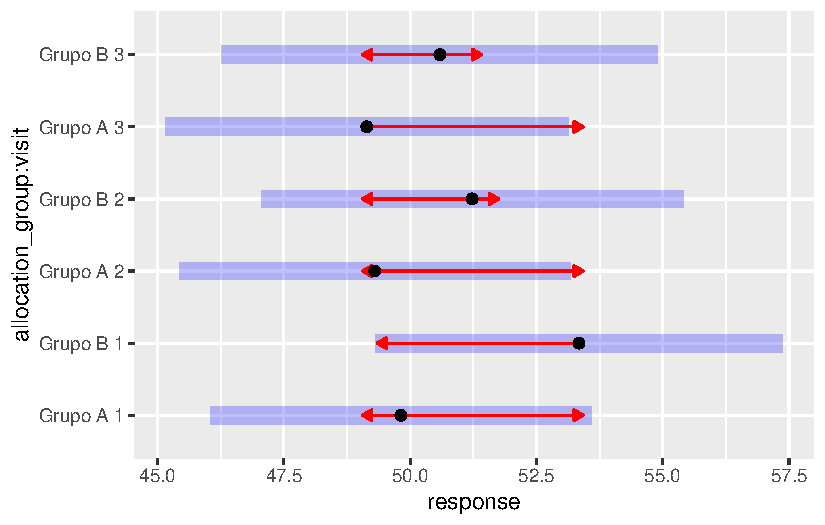
\includegraphics{Outcomes_files/figure-pdf/labs_hdl_sens_emm-1.pdf}

\paragraph{Resultado}\label{resultado-6}

No modelo ajustado para os níveis de HDL-colesterol, não foram
observadas diferenças estatisticamente significativas entre os grupos em
nenhum dos três momentos avaliados. Também não houve mudanças
significativas ao longo do tempo dentro de cada grupo. A análise de
sensibilidade, conduzida com a exclusão das observações influentes, não
alterou substancialmente os resultados. As estimativas permaneceram
consistentes e as comparações entre grupos e ao longo do tempo
continuaram não significativas. As estimativas, intervalos de confiança
de 95\% e valores de p estão apresentados na Tabela~\ref{tbl-hdl}.

\begin{longtable}[]{@{}
  >{\raggedright\arraybackslash}p{(\columnwidth - 8\tabcolsep) * \real{0.2000}}
  >{\raggedright\arraybackslash}p{(\columnwidth - 8\tabcolsep) * \real{0.2000}}
  >{\raggedright\arraybackslash}p{(\columnwidth - 8\tabcolsep) * \real{0.2000}}
  >{\raggedright\arraybackslash}p{(\columnwidth - 8\tabcolsep) * \real{0.2000}}
  >{\raggedright\arraybackslash}p{(\columnwidth - 8\tabcolsep) * \real{0.2000}}@{}}
\caption{Diferenças estimadas dos níveis de HDL-colesterol entre os
grupos de alocação (placebo vs Eclipta) e entre visitas dentro de cada
grupo}\label{tbl-hdl}\tabularnewline
\toprule\noalign{}
\begin{minipage}[b]{\linewidth}\raggedright
Grupo de comparação
\end{minipage} & \begin{minipage}[b]{\linewidth}\raggedright
Comparação
\end{minipage} & \begin{minipage}[b]{\linewidth}\raggedright
Estimativa
\end{minipage} & \begin{minipage}[b]{\linewidth}\raggedright
IC 95\%
\end{minipage} & \begin{minipage}[b]{\linewidth}\raggedright
p-valor
\end{minipage} \\
\midrule\noalign{}
\endfirsthead
\toprule\noalign{}
\begin{minipage}[b]{\linewidth}\raggedright
Grupo de comparação
\end{minipage} & \begin{minipage}[b]{\linewidth}\raggedright
Comparação
\end{minipage} & \begin{minipage}[b]{\linewidth}\raggedright
Estimativa
\end{minipage} & \begin{minipage}[b]{\linewidth}\raggedright
IC 95\%
\end{minipage} & \begin{minipage}[b]{\linewidth}\raggedright
p-valor
\end{minipage} \\
\midrule\noalign{}
\endhead
\bottomrule\noalign{}
\endlastfoot
Entre grupos & Visita 1 & -3,47 & {[}-9,15 ; 2,21{]} & 0,228 \\
Entre grupos & Visita 2 & -2,22 & {[}-8,14 ; 3,69{]} & 0,458 \\
Entre grupos & Visita 3 & -1,71 & {[}-7,83 ; 4,42{]} & 0,582 \\
Grupo Placebo & Visita 1 - Visita 2 & 0,88 & {[}-2,87 ; 4,64{]} &
1,000 \\
Grupo Placebo & Visita 1 - Visita 3 & 0,99 & {[}-3,08 ; 5,05{]} &
1,000 \\
Grupo Placebo & Visita 2 - Visita 3 & 0,10 & {[}-3,96 ; 4,17{]} &
1,000 \\
Grupo Eclipta & Visita 1 - Visita 2 & 2,13 & {[}-2,12 ; 6,38{]} &
0,675 \\
Grupo Eclipta & Visita 1 - Visita 3 & 2,75 & {[}-1,74 ; 7,24{]} &
0,418 \\
Grupo Eclipta & Visita 2 - Visita 3 & 0,62 & {[}-3,99 ; 5,22{]} &
1,000 \\
\end{longtable}

\begin{Shaded}
\begin{Highlighting}[]
\FunctionTok{ggplot}\NormalTok{(}
    \AttributeTok{data =}\NormalTok{ data\_model, }
    \FunctionTok{aes}\NormalTok{(}
        \AttributeTok{x =} \FunctionTok{as.factor}\NormalTok{(visit),}
        \AttributeTok{y =}\NormalTok{ labs\_hdl,}
        \AttributeTok{group =}\NormalTok{ record\_id,}
\NormalTok{    )}
\NormalTok{) }\SpecialCharTok{+}
    \FunctionTok{geom\_line}\NormalTok{(}\AttributeTok{alpha =} \FloatTok{0.5}\NormalTok{) }\SpecialCharTok{+}
    \FunctionTok{geom\_point}\NormalTok{(}\AttributeTok{alpha =} \FloatTok{0.7}\NormalTok{) }\SpecialCharTok{+}
    \FunctionTok{geom\_smooth}\NormalTok{(}
        \FunctionTok{aes}\NormalTok{(}\AttributeTok{group =}\NormalTok{ allocation\_group),}
        \AttributeTok{method =} \StringTok{"lm"}\NormalTok{,}
        \AttributeTok{se =} \ConstantTok{TRUE}\NormalTok{,}
        \AttributeTok{linewidth =} \DecValTok{1}
\NormalTok{    ) }\SpecialCharTok{+}
    \FunctionTok{labs}\NormalTok{(}\AttributeTok{title =} \StringTok{"All data"}\NormalTok{) }\SpecialCharTok{+}
    \FunctionTok{facet\_wrap}\NormalTok{(}\SpecialCharTok{\textasciitilde{}}\NormalTok{ allocation\_group) }
\end{Highlighting}
\end{Shaded}

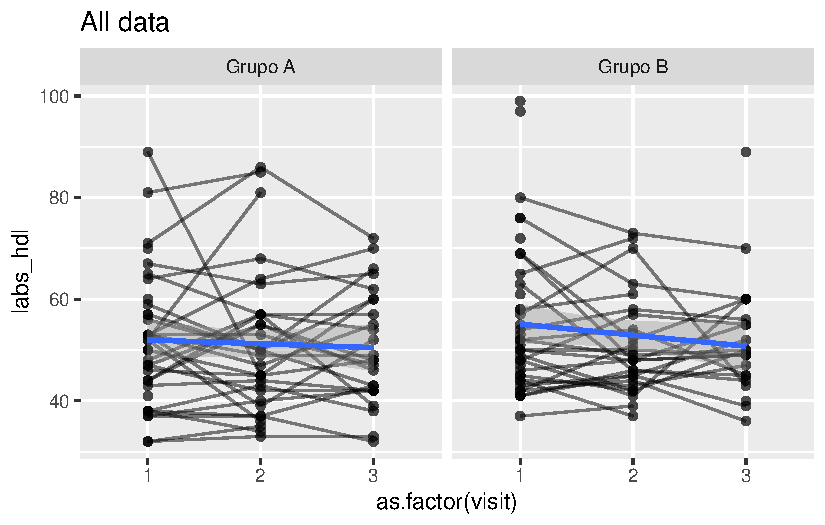
\includegraphics{Outcomes_files/figure-pdf/labs_hdl_6-1.pdf}

\begin{Shaded}
\begin{Highlighting}[]
    \CommentTok{\#coord\_cartesian(ylim = c(10, 150))}

\NormalTok{data\_model }\SpecialCharTok{\%\textgreater{}\%} 
    \FunctionTok{filter}\NormalTok{(}
        \SpecialCharTok{!}\NormalTok{(record\_id }\SpecialCharTok{\%in\%} 
\NormalTok{        labs\_hdl\_model\_check}\SpecialCharTok{$}\NormalTok{influential\_ids)}
\NormalTok{    ) }\SpecialCharTok{\%\textgreater{}\%} 
    \FunctionTok{ggplot}\NormalTok{(}
        \FunctionTok{aes}\NormalTok{(}
            \AttributeTok{x =} \FunctionTok{as.factor}\NormalTok{(visit),}
            \AttributeTok{y =}\NormalTok{ labs\_hdl,}
            \AttributeTok{group =}\NormalTok{ record\_id,}
\NormalTok{        )}
\NormalTok{    ) }\SpecialCharTok{+}
    \FunctionTok{geom\_line}\NormalTok{(}\AttributeTok{alpha =} \FloatTok{0.5}\NormalTok{) }\SpecialCharTok{+}
    \FunctionTok{geom\_point}\NormalTok{(}\AttributeTok{alpha =} \FloatTok{0.7}\NormalTok{) }\SpecialCharTok{+}
    \FunctionTok{geom\_smooth}\NormalTok{(}
        \FunctionTok{aes}\NormalTok{(}\AttributeTok{group =}\NormalTok{ allocation\_group),}
        \AttributeTok{method =} \StringTok{"lm"}\NormalTok{,}
        \AttributeTok{se =} \ConstantTok{TRUE}\NormalTok{,}
        \AttributeTok{linewidth =} \DecValTok{1}
\NormalTok{    ) }\SpecialCharTok{+}
    \FunctionTok{labs}\NormalTok{(}\AttributeTok{title =} \StringTok{"Sensitivity analysis"}\NormalTok{) }\SpecialCharTok{+}
    \FunctionTok{facet\_wrap}\NormalTok{(}\SpecialCharTok{\textasciitilde{}}\NormalTok{ allocation\_group) }
\end{Highlighting}
\end{Shaded}

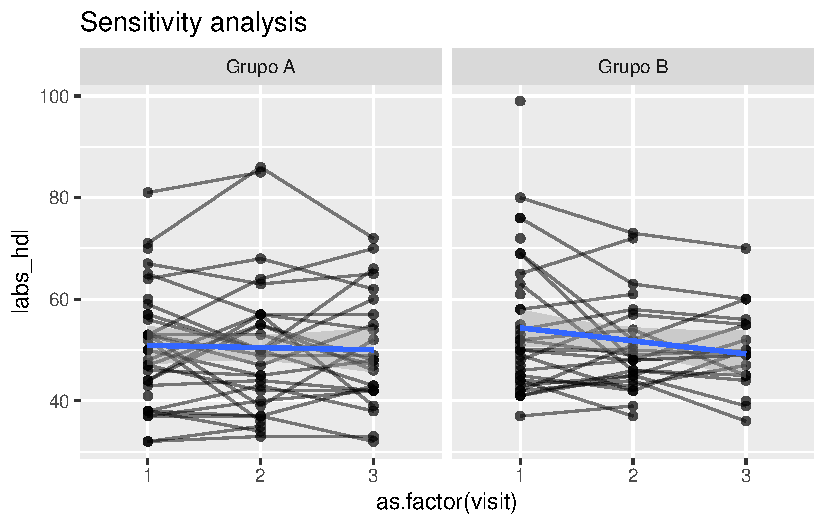
\includegraphics{Outcomes_files/figure-pdf/labs_hdl_6-2.pdf}

\begin{Shaded}
\begin{Highlighting}[]
    \CommentTok{\#coord\_cartesian(ylim = c(10, 150))}
\end{Highlighting}
\end{Shaded}

\subsubsection{Triglicerídeos}\label{trigliceruxeddeos}

Variável: \texttt{labs\_triglycerides}

\begin{Shaded}
\begin{Highlighting}[]
\CommentTok{\# Plot 1: Raw data}
\NormalTok{labs\_triglycerides\_hist\_1 }\OtherTok{\textless{}{-}}\NormalTok{ data\_model }\SpecialCharTok{\%\textgreater{}\%} 
    \CommentTok{\#filter(}
    \CommentTok{\#    labs\_triglycerides \textless{} 300}
    \CommentTok{\#) \%\textgreater{}\% }
    \FunctionTok{ggplot}\NormalTok{(}\FunctionTok{aes}\NormalTok{(}\AttributeTok{x =}\NormalTok{ labs\_triglycerides)) }\SpecialCharTok{+} 
    \FunctionTok{geom\_histogram}\NormalTok{(}\AttributeTok{bins =} \DecValTok{50}\NormalTok{, }\AttributeTok{fill =} \StringTok{"skyblue"}\NormalTok{, }\AttributeTok{color =} \StringTok{"black"}\NormalTok{)}

\CommentTok{\# Plot 2: Log{-}transformed data}
\NormalTok{labs\_triglycerides\_hist\_2 }\OtherTok{\textless{}{-}}\NormalTok{ data\_model }\SpecialCharTok{\%\textgreater{}\%} 
    \CommentTok{\#filter(}
    \CommentTok{\#    labs\_triglycerides \textless{} 300}
    \CommentTok{\#) \%\textgreater{}\%}
    \FunctionTok{ggplot}\NormalTok{(}\FunctionTok{aes}\NormalTok{(}\AttributeTok{x =} \FunctionTok{log1p}\NormalTok{(labs\_triglycerides))) }\SpecialCharTok{+} 
    \FunctionTok{geom\_histogram}\NormalTok{(}\AttributeTok{bins =} \DecValTok{50}\NormalTok{, }\AttributeTok{fill =} \StringTok{"lightgreen"}\NormalTok{, }\AttributeTok{color =} \StringTok{"black"}\NormalTok{)}

\CommentTok{\# Combine side by side}
\NormalTok{labs\_triglycerides\_hist\_1 }\SpecialCharTok{+}\NormalTok{ labs\_triglycerides\_hist\_2 }\CommentTok{\# library(patchwork)}
\end{Highlighting}
\end{Shaded}

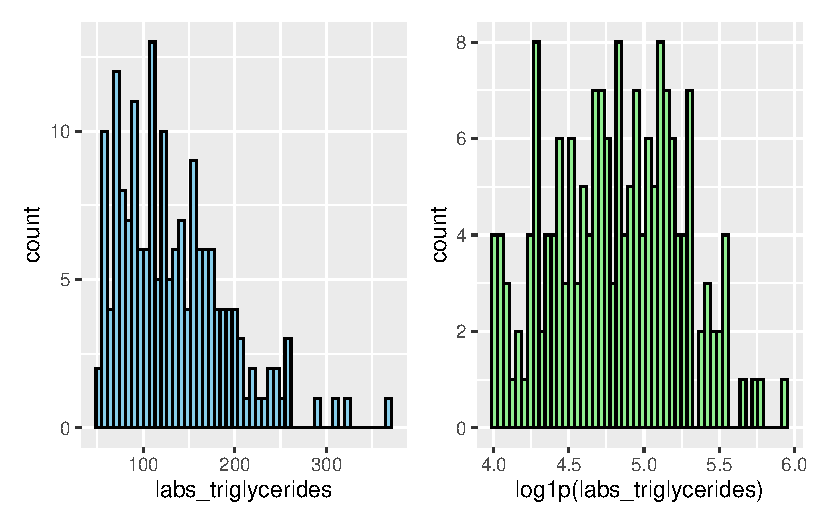
\includegraphics{Outcomes_files/figure-pdf/labs_triglycerides_1-1.pdf}

\begin{Shaded}
\begin{Highlighting}[]
\CommentTok{\# LMM}
\NormalTok{labs\_triglycerides\_model }\OtherTok{\textless{}{-}} \FunctionTok{lmer}\NormalTok{(}\FunctionTok{log1p}\NormalTok{(labs\_triglycerides) }\SpecialCharTok{\textasciitilde{}}\NormalTok{ allocation\_group }\SpecialCharTok{*}\NormalTok{ visit }\SpecialCharTok{+} 
\NormalTok{(}\DecValTok{1} \SpecialCharTok{|}\NormalTok{ record\_id), }\AttributeTok{data =}\NormalTok{ data\_model)}
\FunctionTok{check\_collinearity}\NormalTok{(labs\_triglycerides\_model)}
\end{Highlighting}
\end{Shaded}

\begin{verbatim}
# Check for Multicollinearity

Low Correlation

                   Term  VIF   VIF 95% CI Increased SE Tolerance Tolerance 95% CI
       allocation_group 1.20 [1.08, 1.53]         1.10      0.83     [0.65, 0.93]
                  visit 3.50 [2.79, 4.49]         1.87      0.29     [0.22, 0.36]
 allocation_group:visit 3.82 [3.03, 4.92]         1.95      0.26     [0.20, 0.33]
\end{verbatim}

\begin{Shaded}
\begin{Highlighting}[]
\CommentTok{\# Sensitivity analysis}
\NormalTok{labs\_triglycerides\_model\_check }\OtherTok{\textless{}{-}} \FunctionTok{sensitivity\_check\_lmer}\NormalTok{(}
    \AttributeTok{model =}\NormalTok{ labs\_triglycerides\_model,}
    \AttributeTok{id\_var =} \StringTok{"record\_id"}\NormalTok{,}
    \AttributeTok{top\_n =} \DecValTok{5}\NormalTok{)}

\CommentTok{\# LMM Sensitivity}
\NormalTok{labs\_triglycerides\_model\_sens }\OtherTok{\textless{}{-}} \FunctionTok{update}\NormalTok{(}\AttributeTok{object =}\NormalTok{ labs\_triglycerides\_model,}
                              \AttributeTok{subset =} \SpecialCharTok{!}\NormalTok{(record\_id }\SpecialCharTok{\%in\%} 
\NormalTok{        labs\_triglycerides\_model\_check}\SpecialCharTok{$}\NormalTok{influential\_ids))}
\CommentTok{\# Influential IDS}
\NormalTok{labs\_triglycerides\_model\_check}\SpecialCharTok{$}\NormalTok{influential\_ids}
\end{Highlighting}
\end{Shaded}

\begin{verbatim}
[1] "16" "17" "1"  "2"  "20"
\end{verbatim}

\paragraph{Resumo dos modelos}\label{resumo-dos-modelos-7}

\begin{Shaded}
\begin{Highlighting}[]
\CommentTok{\# Model comparison}
\FunctionTok{summary}\NormalTok{(labs\_triglycerides\_model)}
\end{Highlighting}
\end{Shaded}

\begin{verbatim}
Linear mixed model fit by REML. t-tests use Satterthwaite's method ['lmerModLmerTest']
Formula: log1p(labs_triglycerides) ~ allocation_group * visit + (1 | record_id)
   Data: data_model

REML criterion at convergence: 156.5

Scaled residuals: 
     Min       1Q   Median       3Q      Max 
-2.48575 -0.55624 -0.06875  0.50582  2.77617 

Random effects:
 Groups    Name        Variance Std.Dev.
 record_id (Intercept) 0.12894  0.3591  
 Residual              0.06212  0.2492  
Number of obs: 179, groups:  record_id, 75

Fixed effects:
                                Estimate Std. Error        df t value Pr(>|t|)    
(Intercept)                      4.76585    0.07186 100.80805  66.322   <2e-16 ***
allocation_groupGrupo B         -0.02118    0.10095 100.80805  -0.210    0.834    
visit2                           0.05652    0.06246 103.24903   0.905    0.368    
visit3                           0.00822    0.06765 104.67836   0.122    0.904    
allocation_groupGrupo B:visit2  -0.05643    0.09159 105.09618  -0.616    0.539    
allocation_groupGrupo B:visit3   0.04983    0.09836 106.17407   0.507    0.614    
---
Signif. codes:  0 '***' 0.001 '**' 0.01 '*' 0.05 '.' 0.1 ' ' 1

Correlation of Fixed Effects:
            (Intr) all_GB visit2 visit3 a_GB:2
allctn_grGB -0.712                            
visit2      -0.374  0.266                     
visit3      -0.345  0.246  0.449              
allctn_GB:2  0.255 -0.358 -0.682 -0.306       
allctn_GB:3  0.238 -0.334 -0.309 -0.688  0.433
\end{verbatim}

\begin{Shaded}
\begin{Highlighting}[]
\FunctionTok{summary}\NormalTok{(labs\_triglycerides\_model\_sens)}
\end{Highlighting}
\end{Shaded}

\begin{verbatim}
Linear mixed model fit by REML. t-tests use Satterthwaite's method ['lmerModLmerTest']
Formula: log1p(labs_triglycerides) ~ allocation_group * visit + (1 | record_id)
   Data: data_model
 Subset: !(record_id %in% labs_triglycerides_model_check$influential_ids)

REML criterion at convergence: 110.8

Scaled residuals: 
     Min       1Q   Median       3Q      Max 
-1.56781 -0.62311 -0.09172  0.57450  2.18137 

Random effects:
 Groups    Name        Variance Std.Dev.
 record_id (Intercept) 0.12547  0.3542  
 Residual              0.04498  0.2121  
Number of obs: 164, groups:  record_id, 70

Fixed effects:
                               Estimate Std. Error       df t value Pr(>|t|)    
(Intercept)                     4.74183    0.07187 86.86729  65.980   <2e-16 ***
allocation_groupGrupo B        -0.02502    0.09885 86.86729  -0.253   0.8008    
visit2                          0.04807    0.05702 92.31050   0.843   0.4014    
visit3                         -0.09539    0.06269 93.35327  -1.522   0.1314    
allocation_groupGrupo B:visit2 -0.01744    0.08158 93.47289  -0.214   0.8312    
allocation_groupGrupo B:visit3  0.17857    0.08845 94.22579   2.019   0.0463 *  
---
Signif. codes:  0 '***' 0.001 '**' 0.01 '*' 0.05 '.' 0.1 ' ' 1

Correlation of Fixed Effects:
            (Intr) all_GB visit2 visit3 a_GB:2
allctn_grGB -0.727                            
visit2      -0.333  0.242                     
visit3      -0.303  0.220  0.444              
allctn_GB:2  0.232 -0.320 -0.699 -0.310       
allctn_GB:3  0.214 -0.295 -0.314 -0.709  0.431
\end{verbatim}

\begin{Shaded}
\begin{Highlighting}[]
\NormalTok{labs\_triglycerides\_model\_check}\SpecialCharTok{$}\NormalTok{comparison\_table}
\end{Highlighting}
\end{Shaded}

\begin{verbatim}
# A tibble: 16 x 6
   Model       term                           estimate std.error statistic   p.value
   <chr>       <chr>                             <dbl>     <dbl>     <dbl>     <dbl>
 1 Original    (Intercept)                     4.77       0.0719    66.3    5.68e-85
 2 Sensitivity (Intercept)                     4.74       0.0719    66.0    5.34e-76
 3 Original    allocation_groupGrupo B        -0.0212     0.101     -0.210  8.34e- 1
 4 Sensitivity allocation_groupGrupo B        -0.0250     0.0989    -0.253  8.01e- 1
 5 Original    allocation_groupGrupo B:visit2 -0.0564     0.0916    -0.616  5.39e- 1
 6 Sensitivity allocation_groupGrupo B:visit2 -0.0174     0.0816    -0.214  8.31e- 1
 7 Original    allocation_groupGrupo B:visit3  0.0498     0.0984     0.507  6.14e- 1
 8 Sensitivity allocation_groupGrupo B:visit3  0.179      0.0884     2.02   4.63e- 2
 9 Original    sd__(Intercept)                 0.359     NA         NA     NA       
10 Sensitivity sd__(Intercept)                 0.354     NA         NA     NA       
11 Original    sd__Observation                 0.249     NA         NA     NA       
12 Sensitivity sd__Observation                 0.212     NA         NA     NA       
13 Original    visit2                          0.0565     0.0625     0.905  3.68e- 1
14 Sensitivity visit2                          0.0481     0.0570     0.843  4.01e- 1
15 Original    visit3                          0.00822    0.0677     0.122  9.04e- 1
16 Sensitivity visit3                         -0.0954     0.0627    -1.52   1.31e- 1
\end{verbatim}

\begin{Shaded}
\begin{Highlighting}[]
\NormalTok{performance}\SpecialCharTok{::}\FunctionTok{compare\_performance}\NormalTok{(}
\NormalTok{    labs\_triglycerides\_model, }
\NormalTok{    labs\_triglycerides\_model\_sens) }
\end{Highlighting}
\end{Shaded}

\begin{verbatim}
# Comparison of Model Performance Indices

Name                          |           Model |  AIC (weights) | AICc (weights) |  BIC (weights) | R2 (cond.) | R2 (marg.) |   ICC |  RMSE | Sigma
----------------------------------------------------------------------------------------------------------------------------------------------------
labs_triglycerides_model      | lmerModLmerTest | 1873.1 (<.001) | 1873.9 (<.001) | 1898.6 (<.001) |      0.676 |      0.004 | 0.675 | 0.199 | 0.249
labs_triglycerides_model_sens | lmerModLmerTest | 1671.7 (>.999) | 1672.6 (>.999) | 1696.5 (>.999) |      0.739 |      0.012 | 0.736 | 0.166 | 0.212
\end{verbatim}

\begin{Shaded}
\begin{Highlighting}[]
\NormalTok{performance}\SpecialCharTok{::}\FunctionTok{check\_model}\NormalTok{(labs\_triglycerides\_model)}
\end{Highlighting}
\end{Shaded}

\includegraphics{Outcomes_files/figure-pdf/labs_triglycerides_4-1.pdf}

\begin{Shaded}
\begin{Highlighting}[]
\NormalTok{performance}\SpecialCharTok{::}\FunctionTok{check\_model}\NormalTok{(labs\_triglycerides\_model\_sens)}
\end{Highlighting}
\end{Shaded}

\includegraphics{Outcomes_files/figure-pdf/labs_triglycerides_4-2.pdf}

\paragraph{Médias Marginais
Estimadas}\label{muxe9dias-marginais-estimadas-7}

\subparagraph{Todos os dados}\label{todos-os-dados-7}

\begin{Shaded}
\begin{Highlighting}[]
\CommentTok{\# Get EMMs for each group at each visit}
\NormalTok{labs\_triglycerides\_raw\_emm }\OtherTok{\textless{}{-}}\NormalTok{ emmeans}\SpecialCharTok{::}\FunctionTok{emmeans}\NormalTok{(}
\NormalTok{    labs\_triglycerides\_model, }
    \SpecialCharTok{\textasciitilde{}}\NormalTok{ allocation\_group }\SpecialCharTok{*}\NormalTok{ visit}
\NormalTok{)}

\NormalTok{labs\_triglycerides\_raw\_emm }\OtherTok{\textless{}{-}} \FunctionTok{regrid}\NormalTok{(labs\_triglycerides\_raw\_emm)}

\CommentTok{\# Table of marginal means}
\CommentTok{\# labs\_triglycerides\_raw\_emm}

\CommentTok{\# Pairwise comparisons: Between groups at each visit}
\NormalTok{emmeans}\SpecialCharTok{::}\FunctionTok{contrast}\NormalTok{(labs\_triglycerides\_raw\_emm,}
\AttributeTok{method =} \StringTok{"pairwise"}\NormalTok{, }\AttributeTok{by =} \StringTok{"visit"}\NormalTok{,}
\AttributeTok{adjust =} \StringTok{"bonferroni"}\NormalTok{) }\SpecialCharTok{\%\textgreater{}\%} \FunctionTok{summary}\NormalTok{(}\AttributeTok{infer =} \FunctionTok{c}\NormalTok{(}\ConstantTok{TRUE}\NormalTok{, }\ConstantTok{TRUE}\NormalTok{))}
\end{Highlighting}
\end{Shaded}

\begin{verbatim}
visit = 1:
 contrast          estimate   SE  df lower.CL upper.CL t.ratio p.value
 Grupo A - Grupo B     2.46 11.7 103    -20.8     25.7   0.210  0.8343

visit = 2:
 contrast          estimate   SE  df lower.CL upper.CL t.ratio p.value
 Grupo A - Grupo B     9.28 13.1 116    -16.6     35.2   0.710  0.4793

visit = 3:
 contrast          estimate   SE  df lower.CL upper.CL t.ratio p.value
 Grupo A - Grupo B    -3.44 13.8 133    -30.8     23.9  -0.249  0.8041

Degrees-of-freedom method: inherited from kenward-roger when re-gridding 
Confidence level used: 0.95 
\end{verbatim}

\begin{Shaded}
\begin{Highlighting}[]
\CommentTok{\# Pairwise comparisons: Changes over time within each group}
\NormalTok{emmeans}\SpecialCharTok{::}\FunctionTok{contrast}\NormalTok{(labs\_triglycerides\_raw\_emm,}
\AttributeTok{method =} \StringTok{"pairwise"}\NormalTok{, }\AttributeTok{by =} \StringTok{"allocation\_group"}\NormalTok{,}
\AttributeTok{adjust =} \StringTok{"bonferroni"}\NormalTok{) }\SpecialCharTok{\%\textgreater{}\%} \FunctionTok{summary}\NormalTok{(}\AttributeTok{infer =} \FunctionTok{c}\NormalTok{(}\ConstantTok{TRUE}\NormalTok{, }\ConstantTok{TRUE}\NormalTok{))}
\end{Highlighting}
\end{Shaded}

\begin{verbatim}
allocation_group = Grupo A:
 contrast        estimate   SE  df lower.CL upper.CL t.ratio p.value
 visit1 - visit2 -6.82768 7.60 103    -25.3     11.7  -0.899  1.0000
 visit1 - visit3 -0.96930 8.00 103    -20.4     18.5  -0.121  1.0000
 visit2 - visit3  5.85838 8.29 116    -14.3     26.0   0.707  1.0000

allocation_group = Grupo B:
 contrast        estimate   SE  df lower.CL upper.CL t.ratio p.value
 visit1 - visit2 -0.00919 7.71 103    -18.8     18.8  -0.001  1.0000
 visit1 - visit3 -6.87130 8.57 103    -27.7     14.0  -0.802  1.0000
 visit2 - visit3 -6.86211 8.90 132    -28.4     14.7  -0.771  1.0000

Degrees-of-freedom method: inherited from kenward-roger when re-gridding 
Confidence level used: 0.95 
Conf-level adjustment: bonferroni method for 3 estimates 
P value adjustment: bonferroni method for 3 tests 
\end{verbatim}

\begin{Shaded}
\begin{Highlighting}[]
\CommentTok{\# Plot of marginal means}
\FunctionTok{plot}\NormalTok{(labs\_triglycerides\_raw\_emm, }\AttributeTok{comparisons =} \ConstantTok{TRUE}\NormalTok{)}
\end{Highlighting}
\end{Shaded}

\includegraphics{Outcomes_files/figure-pdf/labs_triglycerides_raw_emm-1.pdf}

\subparagraph{Análise de
sensibilidade}\label{anuxe1lise-de-sensibilidade-7}

\begin{Shaded}
\begin{Highlighting}[]
\CommentTok{\# Get EMMs for each group at each visit (Sensitivity Analysis)}
\NormalTok{labs\_triglycerides\_emm }\OtherTok{\textless{}{-}}\NormalTok{ emmeans}\SpecialCharTok{::}\FunctionTok{emmeans}\NormalTok{(}
\NormalTok{    labs\_triglycerides\_model\_sens, }
    \SpecialCharTok{\textasciitilde{}}\NormalTok{ allocation\_group }\SpecialCharTok{*}\NormalTok{ visit}
\NormalTok{)}

\NormalTok{labs\_triglycerides\_emm }\OtherTok{\textless{}{-}} \FunctionTok{regrid}\NormalTok{(labs\_triglycerides\_emm)}

\CommentTok{\# Table of marginal means}
\CommentTok{\# labs\_triglycerides\_emm}

\CommentTok{\# Pairwise comparisons: Between groups at each visit}
\NormalTok{emmeans}\SpecialCharTok{::}\FunctionTok{contrast}\NormalTok{(labs\_triglycerides\_emm,}
\AttributeTok{method =} \StringTok{"pairwise"}\NormalTok{, }\AttributeTok{by =} \StringTok{"visit"}\NormalTok{,}
\AttributeTok{adjust =} \StringTok{"bonferroni"}\NormalTok{) }\SpecialCharTok{\%\textgreater{}\%} \FunctionTok{summary}\NormalTok{(}\AttributeTok{infer =} \FunctionTok{c}\NormalTok{(}\ConstantTok{TRUE}\NormalTok{, }\ConstantTok{TRUE}\NormalTok{))}
\end{Highlighting}
\end{Shaded}

\begin{verbatim}
visit = 1:
 contrast          estimate   SE    df lower.CL upper.CL t.ratio p.value
 Grupo A - Grupo B     2.83 11.2  88.9    -19.4    25.09   0.253  0.8010

visit = 2:
 contrast          estimate   SE    df lower.CL upper.CL t.ratio p.value
 Grupo A - Grupo B     5.00 12.5 101.6    -19.8    29.83   0.399  0.6904

visit = 3:
 contrast          estimate   SE    df lower.CL upper.CL t.ratio p.value
 Grupo A - Grupo B   -17.30 12.6 117.7    -42.3     7.68  -1.371  0.1729

Degrees-of-freedom method: inherited from kenward-roger when re-gridding 
Confidence level used: 0.95 
\end{verbatim}

\begin{Shaded}
\begin{Highlighting}[]
\CommentTok{\# Pairwise comparisons: Changes over time within each group}
\NormalTok{emmeans}\SpecialCharTok{::}\FunctionTok{contrast}\NormalTok{(labs\_triglycerides\_emm,}
\AttributeTok{method =} \StringTok{"pairwise"}\NormalTok{, }\AttributeTok{by =} \StringTok{"allocation\_group"}\NormalTok{,}
\AttributeTok{adjust =} \StringTok{"bonferroni"}\NormalTok{) }\SpecialCharTok{\%\textgreater{}\%} \FunctionTok{summary}\NormalTok{(}\AttributeTok{infer =} \FunctionTok{c}\NormalTok{(}\ConstantTok{TRUE}\NormalTok{, }\ConstantTok{TRUE}\NormalTok{))}
\end{Highlighting}
\end{Shaded}

\begin{verbatim}
allocation_group = Grupo A:
 contrast        estimate   SE    df lower.CL upper.CL t.ratio p.value
 visit1 - visit2    -5.65 6.74  88.9   -22.10    10.81  -0.837  1.0000
 visit1 - visit3    10.43 6.81  88.9    -6.17    27.04   1.533  0.3866
 visit2 - visit3    16.08 7.12 101.6    -1.25    33.40   2.259  0.0780

allocation_group = Grupo B:
 contrast        estimate   SE    df lower.CL upper.CL t.ratio p.value
 visit1 - visit2    -3.48 6.67  88.9   -19.75    12.79  -0.522  1.0000
 visit1 - visit3    -9.70 7.43  88.9   -27.83     8.44  -1.305  0.5861
 visit2 - visit3    -6.22 7.76 114.3   -25.07    12.63  -0.802  1.0000

Degrees-of-freedom method: inherited from kenward-roger when re-gridding 
Confidence level used: 0.95 
Conf-level adjustment: bonferroni method for 3 estimates 
P value adjustment: bonferroni method for 3 tests 
\end{verbatim}

\begin{Shaded}
\begin{Highlighting}[]
\CommentTok{\# Plot of marginal means}
\FunctionTok{plot}\NormalTok{(labs\_triglycerides\_emm, }\AttributeTok{comparisons =} \ConstantTok{TRUE}\NormalTok{)}
\end{Highlighting}
\end{Shaded}

\includegraphics{Outcomes_files/figure-pdf/labs_triglycerides_sens_emm-1.pdf}

\paragraph{Resultado}\label{resultado-7}

No modelo ajustado para os níveis de triglicerídeos, não foram
observadas diferenças estatisticamente significativas entre os grupos em
nenhum dos três momentos avaliados. As estimativas entre grupos foram
próximas de zero e os intervalos de confiança incluíram o valor nulo,
com valores de p superiores a 0,47 em todas as comparações. Da mesma
forma, as comparações intragrupo ao longo do tempo não revelaram
mudanças significativas em nenhum dos grupos, embora tenha havido uma
tendência não significativa de aumento entre a visita 2 e a visita 3 no
grupo A (p = 0,078).

A análise de sensibilidade, realizada após a exclusão de observações
influentes, manteve os resultados essencialmente inalterados. As
estimativas permaneceram próximas das observadas no modelo completo e
não houve modificações relevantes nas interpretações. As estimativas,
intervalos de confiança de 95\% e valores de p estão apresentados na
Tabela~\ref{tbl-triglycerides}.

\begin{longtable}[]{@{}
  >{\raggedright\arraybackslash}p{(\columnwidth - 8\tabcolsep) * \real{0.2000}}
  >{\raggedright\arraybackslash}p{(\columnwidth - 8\tabcolsep) * \real{0.2000}}
  >{\raggedright\arraybackslash}p{(\columnwidth - 8\tabcolsep) * \real{0.2000}}
  >{\raggedright\arraybackslash}p{(\columnwidth - 8\tabcolsep) * \real{0.2000}}
  >{\raggedright\arraybackslash}p{(\columnwidth - 8\tabcolsep) * \real{0.2000}}@{}}
\caption{Diferenças estimadas dos níveis de triglicerídeos entre os
grupos de alocação (placebo vs Eclipta) e entre visitas dentro de cada
grupo}\label{tbl-triglycerides}\tabularnewline
\toprule\noalign{}
\begin{minipage}[b]{\linewidth}\raggedright
Grupo de comparação
\end{minipage} & \begin{minipage}[b]{\linewidth}\raggedright
Comparação
\end{minipage} & \begin{minipage}[b]{\linewidth}\raggedright
Estimativa
\end{minipage} & \begin{minipage}[b]{\linewidth}\raggedright
IC 95\%
\end{minipage} & \begin{minipage}[b]{\linewidth}\raggedright
p-valor
\end{minipage} \\
\midrule\noalign{}
\endfirsthead
\toprule\noalign{}
\begin{minipage}[b]{\linewidth}\raggedright
Grupo de comparação
\end{minipage} & \begin{minipage}[b]{\linewidth}\raggedright
Comparação
\end{minipage} & \begin{minipage}[b]{\linewidth}\raggedright
Estimativa
\end{minipage} & \begin{minipage}[b]{\linewidth}\raggedright
IC 95\%
\end{minipage} & \begin{minipage}[b]{\linewidth}\raggedright
p-valor
\end{minipage} \\
\midrule\noalign{}
\endhead
\bottomrule\noalign{}
\endlastfoot
Entre grupos & Visita 1 & 2,46 & {[}-20,8 ; 25,7{]} & 0,834 \\
Entre grupos & Visita 2 & 9,28 & {[}-16,6 ; 35,2{]} & 0,479 \\
Entre grupos & Visita 3 & -3,44 & {[}-30,8 ; 23,9{]} & 0,804 \\
Grupo Placebo & Visita 1 - Visita 2 & -6,83 & {[}-25,3 ; 11,7{]} &
1,000 \\
Grupo Placebo & Visita 1 - Visita 3 & -0,97 & {[}-20,4 ; 18,5{]} &
1,000 \\
Grupo Placebo & Visita 2 - Visita 3 & 5,86 & {[}-14,3 ; 26,0{]} &
1,000 \\
Grupo Eclipta & Visita 1 - Visita 2 & -0,01 & {[}-18,8 ; 18,8{]} &
1,000 \\
Grupo Eclipta & Visita 1 - Visita 3 & -6,87 & {[}-27,7 ; 14,0{]} &
1,000 \\
Grupo Eclipta & Visita 2 - Visita 3 & -6,86 & {[}-28,4 ; 14,7{]} &
1,000 \\
\end{longtable}

\begin{Shaded}
\begin{Highlighting}[]
\FunctionTok{ggplot}\NormalTok{(}
    \AttributeTok{data =}\NormalTok{ data\_model, }
    \FunctionTok{aes}\NormalTok{(}
        \AttributeTok{x =} \FunctionTok{as.factor}\NormalTok{(visit),}
        \AttributeTok{y =}\NormalTok{ labs\_triglycerides,}
        \AttributeTok{group =}\NormalTok{ record\_id,}
\NormalTok{    )}
\NormalTok{) }\SpecialCharTok{+}
    \FunctionTok{geom\_line}\NormalTok{(}\AttributeTok{alpha =} \FloatTok{0.5}\NormalTok{) }\SpecialCharTok{+}
    \FunctionTok{geom\_point}\NormalTok{(}\AttributeTok{alpha =} \FloatTok{0.7}\NormalTok{) }\SpecialCharTok{+}
    \FunctionTok{geom\_smooth}\NormalTok{(}
        \FunctionTok{aes}\NormalTok{(}\AttributeTok{group =}\NormalTok{ allocation\_group),}
        \AttributeTok{method =} \StringTok{"lm"}\NormalTok{,}
        \AttributeTok{se =} \ConstantTok{TRUE}\NormalTok{,}
        \AttributeTok{linewidth =} \DecValTok{1}
\NormalTok{    ) }\SpecialCharTok{+}
    \FunctionTok{labs}\NormalTok{(}\AttributeTok{title =} \StringTok{"All data"}\NormalTok{) }\SpecialCharTok{+}
    \FunctionTok{facet\_wrap}\NormalTok{(}\SpecialCharTok{\textasciitilde{}}\NormalTok{ allocation\_group) }
\end{Highlighting}
\end{Shaded}

\includegraphics{Outcomes_files/figure-pdf/labs_triglycerides_6-1.pdf}

\begin{Shaded}
\begin{Highlighting}[]
    \CommentTok{\#coord\_cartesian(ylim = c(10, 150))}

\NormalTok{data\_model }\SpecialCharTok{\%\textgreater{}\%} 
    \FunctionTok{filter}\NormalTok{(}
        \SpecialCharTok{!}\NormalTok{(record\_id }\SpecialCharTok{\%in\%} 
\NormalTok{        labs\_triglycerides\_model\_check}\SpecialCharTok{$}\NormalTok{influential\_ids)}
\NormalTok{    ) }\SpecialCharTok{\%\textgreater{}\%} 
    \FunctionTok{ggplot}\NormalTok{(}
        \FunctionTok{aes}\NormalTok{(}
            \AttributeTok{x =} \FunctionTok{as.factor}\NormalTok{(visit),}
            \AttributeTok{y =}\NormalTok{ labs\_triglycerides,}
            \AttributeTok{group =}\NormalTok{ record\_id,}
\NormalTok{        )}
\NormalTok{    ) }\SpecialCharTok{+}
    \FunctionTok{geom\_line}\NormalTok{(}\AttributeTok{alpha =} \FloatTok{0.5}\NormalTok{) }\SpecialCharTok{+}
    \FunctionTok{geom\_point}\NormalTok{(}\AttributeTok{alpha =} \FloatTok{0.7}\NormalTok{) }\SpecialCharTok{+}
    \FunctionTok{geom\_smooth}\NormalTok{(}
        \FunctionTok{aes}\NormalTok{(}\AttributeTok{group =}\NormalTok{ allocation\_group),}
        \AttributeTok{method =} \StringTok{"lm"}\NormalTok{,}
        \AttributeTok{se =} \ConstantTok{TRUE}\NormalTok{,}
        \AttributeTok{linewidth =} \DecValTok{1}
\NormalTok{    ) }\SpecialCharTok{+}
    \FunctionTok{labs}\NormalTok{(}\AttributeTok{title =} \StringTok{"Sensitivity analysis"}\NormalTok{) }\SpecialCharTok{+}
    \FunctionTok{facet\_wrap}\NormalTok{(}\SpecialCharTok{\textasciitilde{}}\NormalTok{ allocation\_group) }
\end{Highlighting}
\end{Shaded}

\includegraphics{Outcomes_files/figure-pdf/labs_triglycerides_6-2.pdf}

\begin{Shaded}
\begin{Highlighting}[]
    \CommentTok{\#coord\_cartesian(ylim = c(10, 150))}
\end{Highlighting}
\end{Shaded}

\subsubsection{Glicemia de jejum}\label{glicemia-de-jejum}

Variável: \texttt{labs\_glucose}

\begin{Shaded}
\begin{Highlighting}[]
\CommentTok{\# Plot 1: Raw data}
\NormalTok{labs\_glucose\_hist\_1 }\OtherTok{\textless{}{-}}\NormalTok{ data\_model }\SpecialCharTok{\%\textgreater{}\%} 
    \CommentTok{\#filter(}
    \CommentTok{\#    labs\_glucose \textless{} 140}
    \CommentTok{\#) \%\textgreater{}\% }
    \FunctionTok{ggplot}\NormalTok{(}\FunctionTok{aes}\NormalTok{(}\AttributeTok{x =}\NormalTok{ labs\_glucose)) }\SpecialCharTok{+} 
    \FunctionTok{geom\_histogram}\NormalTok{(}\AttributeTok{bins =} \DecValTok{50}\NormalTok{, }\AttributeTok{fill =} \StringTok{"skyblue"}\NormalTok{, }\AttributeTok{color =} \StringTok{"black"}\NormalTok{)}

\CommentTok{\# Plot 2: Log{-}transformed data}
\NormalTok{labs\_glucose\_hist\_2 }\OtherTok{\textless{}{-}}\NormalTok{ data\_model }\SpecialCharTok{\%\textgreater{}\%} 
    \CommentTok{\#filter(}
    \CommentTok{\#    labs\_glucose \textless{} 140}
    \CommentTok{\#) \%\textgreater{}\%}
    \FunctionTok{ggplot}\NormalTok{(}\FunctionTok{aes}\NormalTok{(}\AttributeTok{x =} \FunctionTok{log1p}\NormalTok{(labs\_glucose))) }\SpecialCharTok{+} 
    \FunctionTok{geom\_histogram}\NormalTok{(}\AttributeTok{bins =} \DecValTok{50}\NormalTok{, }\AttributeTok{fill =} \StringTok{"lightgreen"}\NormalTok{, }\AttributeTok{color =} \StringTok{"black"}\NormalTok{)}

\CommentTok{\# Combine side by side}
\NormalTok{labs\_glucose\_hist\_1 }\SpecialCharTok{+}\NormalTok{ labs\_glucose\_hist\_2 }\CommentTok{\# library(patchwork)}
\end{Highlighting}
\end{Shaded}

\includegraphics{Outcomes_files/figure-pdf/labs_glucose_1-1.pdf}

\begin{Shaded}
\begin{Highlighting}[]
\CommentTok{\# LMM}
\NormalTok{labs\_glucose\_model }\OtherTok{\textless{}{-}} \FunctionTok{lmer}\NormalTok{(}\FunctionTok{log1p}\NormalTok{(labs\_glucose) }\SpecialCharTok{\textasciitilde{}}\NormalTok{ allocation\_group }\SpecialCharTok{*}\NormalTok{ visit }\SpecialCharTok{+} 
\NormalTok{(}\DecValTok{1} \SpecialCharTok{|}\NormalTok{ record\_id), }\AttributeTok{data =}\NormalTok{ data\_model)}
\FunctionTok{check\_collinearity}\NormalTok{(labs\_glucose\_model)}
\end{Highlighting}
\end{Shaded}

\begin{verbatim}
# Check for Multicollinearity

Low Correlation

                   Term  VIF   VIF 95% CI Increased SE Tolerance Tolerance 95% CI
       allocation_group 1.13 [1.03, 1.51]         1.06      0.89     [0.66, 0.97]
                  visit 3.47 [2.76, 4.47]         1.86      0.29     [0.22, 0.36]
 allocation_group:visit 3.69 [2.93, 4.75]         1.92      0.27     [0.21, 0.34]
\end{verbatim}

\begin{Shaded}
\begin{Highlighting}[]
\CommentTok{\# Sensitivity analysis}
\NormalTok{labs\_glucose\_model\_check }\OtherTok{\textless{}{-}} \FunctionTok{sensitivity\_check\_lmer}\NormalTok{(}
    \AttributeTok{model =}\NormalTok{ labs\_glucose\_model,}
    \AttributeTok{id\_var =} \StringTok{"record\_id"}\NormalTok{,}
    \AttributeTok{top\_n =} \DecValTok{5}\NormalTok{)}

\CommentTok{\# LMM Sensitivity}
\NormalTok{labs\_glucose\_model\_sens }\OtherTok{\textless{}{-}} \FunctionTok{update}\NormalTok{(}\AttributeTok{object =}\NormalTok{ labs\_glucose\_model,}
                              \AttributeTok{subset =} \SpecialCharTok{!}\NormalTok{(record\_id }\SpecialCharTok{\%in\%} 
\NormalTok{        labs\_glucose\_model\_check}\SpecialCharTok{$}\NormalTok{influential\_ids))}
\CommentTok{\# Influential IDS}
\NormalTok{labs\_glucose\_model\_check}\SpecialCharTok{$}\NormalTok{influential\_ids}
\end{Highlighting}
\end{Shaded}

\begin{verbatim}
[1] "2"  "16" "17" "56" "13"
\end{verbatim}

\paragraph{Resumo dos modelos}\label{resumo-dos-modelos-8}

\begin{Shaded}
\begin{Highlighting}[]
\CommentTok{\# Model comparison}
\FunctionTok{summary}\NormalTok{(labs\_glucose\_model)}
\end{Highlighting}
\end{Shaded}

\begin{verbatim}
Linear mixed model fit by REML. t-tests use Satterthwaite's method ['lmerModLmerTest']
Formula: log1p(labs_glucose) ~ allocation_group * visit + (1 | record_id)
   Data: data_model

REML criterion at convergence: -153

Scaled residuals: 
    Min      1Q  Median      3Q     Max 
-2.0712 -0.5250 -0.1192  0.4737  3.4423 

Random effects:
 Groups    Name        Variance Std.Dev.
 record_id (Intercept) 0.030440 0.17447 
 Residual              0.008319 0.09121 
Number of obs: 176, groups:  record_id, 74

Fixed effects:
                                 Estimate Std. Error         df t value Pr(>|t|)    
(Intercept)                      4.445812   0.032366  92.773372 137.362   <2e-16 ***
allocation_groupGrupo B          0.002937   0.045895  93.526588   0.064    0.949    
visit2                           0.009144   0.023244 104.438133   0.393    0.695    
visit3                           0.035792   0.024905 105.095812   1.437    0.154    
allocation_groupGrupo B:visit2  -0.019077   0.034014 105.360265  -0.561    0.576    
allocation_groupGrupo B:visit3  -0.007509   0.036617 106.709642  -0.205    0.838    
---
Signif. codes:  0 '***' 0.001 '**' 0.01 '*' 0.05 '.' 0.1 ' ' 1

Correlation of Fixed Effects:
            (Intr) all_GB visit2 visit3 a_GB:2
allctn_grGB -0.705                            
visit2      -0.299  0.211                     
visit3      -0.279  0.197  0.445              
allctn_GB:2  0.204 -0.293 -0.683 -0.304       
allctn_GB:3  0.190 -0.278 -0.303 -0.680  0.439
\end{verbatim}

\begin{Shaded}
\begin{Highlighting}[]
\FunctionTok{summary}\NormalTok{(labs\_glucose\_model\_sens)}
\end{Highlighting}
\end{Shaded}

\begin{verbatim}
Linear mixed model fit by REML. t-tests use Satterthwaite's method ['lmerModLmerTest']
Formula: log1p(labs_glucose) ~ allocation_group * visit + (1 | record_id)
   Data: data_model
 Subset: !(record_id %in% labs_glucose_model_check$influential_ids)

REML criterion at convergence: -224.4

Scaled residuals: 
    Min      1Q  Median      3Q     Max 
-1.9874 -0.5692 -0.1200  0.5703  1.9303 

Random effects:
 Groups    Name        Variance Std.Dev.
 record_id (Intercept) 0.011973 0.10942 
 Residual              0.005831 0.07636 
Number of obs: 161, groups:  record_id, 69

Fixed effects:
                                 Estimate Std. Error         df t value Pr(>|t|)    
(Intercept)                     4.4198168  0.0228838 96.3391006 193.142   <2e-16 ***
allocation_groupGrupo B        -0.0005277  0.0322590 97.2962023  -0.016    0.987    
visit2                         -0.0018470  0.0203795 96.0503867  -0.091    0.928    
visit3                          0.0190546  0.0220059 97.1965932   0.866    0.389    
allocation_groupGrupo B:visit2 -0.0022058  0.0295835 97.2662772  -0.075    0.941    
allocation_groupGrupo B:visit3  0.0099619  0.0320363 99.3466017   0.311    0.756    
---
Signif. codes:  0 '***' 0.001 '**' 0.01 '*' 0.05 '.' 0.1 ' ' 1

Correlation of Fixed Effects:
            (Intr) all_GB visit2 visit3 a_GB:2
allctn_grGB -0.709                            
visit2      -0.368  0.261                     
visit3      -0.341  0.242  0.435              
allctn_GB:2  0.253 -0.360 -0.689 -0.300       
allctn_GB:3  0.234 -0.339 -0.299 -0.687  0.428
\end{verbatim}

\begin{Shaded}
\begin{Highlighting}[]
\NormalTok{labs\_glucose\_model\_check}\SpecialCharTok{$}\NormalTok{comparison\_table}
\end{Highlighting}
\end{Shaded}

\begin{verbatim}
# A tibble: 16 x 6
   Model       term                            estimate std.error statistic    p.value
   <chr>       <chr>                              <dbl>     <dbl>     <dbl>      <dbl>
 1 Original    (Intercept)                     4.45        0.0324  137.      5.55e-109
 2 Sensitivity (Intercept)                     4.42        0.0229  193.      1.57e-126
 3 Original    allocation_groupGrupo B         0.00294     0.0459    0.0640  9.49e-  1
 4 Sensitivity allocation_groupGrupo B        -0.000528    0.0323   -0.0164  9.87e-  1
 5 Original    allocation_groupGrupo B:visit2 -0.0191      0.0340   -0.561   5.76e-  1
 6 Sensitivity allocation_groupGrupo B:visit2 -0.00221     0.0296   -0.0746  9.41e-  1
 7 Original    allocation_groupGrupo B:visit3 -0.00751     0.0366   -0.205   8.38e-  1
 8 Sensitivity allocation_groupGrupo B:visit3  0.00996     0.0320    0.311   7.56e-  1
 9 Original    sd__(Intercept)                 0.174      NA        NA      NA        
10 Sensitivity sd__(Intercept)                 0.109      NA        NA      NA        
11 Original    sd__Observation                 0.0912     NA        NA      NA        
12 Sensitivity sd__Observation                 0.0764     NA        NA      NA        
13 Original    visit2                          0.00914     0.0232    0.393   6.95e-  1
14 Sensitivity visit2                         -0.00185     0.0204   -0.0906  9.28e-  1
15 Original    visit3                          0.0358      0.0249    1.44    1.54e-  1
16 Sensitivity visit3                          0.0191      0.0220    0.866   3.89e-  1
\end{verbatim}

\begin{Shaded}
\begin{Highlighting}[]
\NormalTok{performance}\SpecialCharTok{::}\FunctionTok{compare\_performance}\NormalTok{(}
\NormalTok{    labs\_glucose\_model, }
\NormalTok{    labs\_glucose\_model\_sens) }
\end{Highlighting}
\end{Shaded}

\begin{verbatim}
# Comparison of Model Performance Indices

Name                    |           Model |  AIC (weights) | AICc (weights) |  BIC (weights) | R2 (cond.) | R2 (marg.) |   ICC |  RMSE | Sigma
----------------------------------------------------------------------------------------------------------------------------------------------
labs_glucose_model      | lmerModLmerTest | 1404.0 (<.001) | 1404.9 (<.001) | 1429.4 (<.001) |      0.787 |      0.006 | 0.785 | 0.071 | 0.091
labs_glucose_model_sens | lmerModLmerTest | 1183.8 (>.999) | 1184.7 (>.999) | 1208.4 (>.999) |      0.675 |      0.007 | 0.672 | 0.061 | 0.076
\end{verbatim}

\begin{Shaded}
\begin{Highlighting}[]
\NormalTok{performance}\SpecialCharTok{::}\FunctionTok{check\_model}\NormalTok{(labs\_glucose\_model)}
\end{Highlighting}
\end{Shaded}

\includegraphics{Outcomes_files/figure-pdf/labs_glucose_4-1.pdf}

\begin{Shaded}
\begin{Highlighting}[]
\NormalTok{performance}\SpecialCharTok{::}\FunctionTok{check\_model}\NormalTok{(labs\_glucose\_model\_sens)}
\end{Highlighting}
\end{Shaded}

\includegraphics{Outcomes_files/figure-pdf/labs_glucose_4-2.pdf}

\paragraph{Médias Marginais
Estimadas}\label{muxe9dias-marginais-estimadas-8}

\subparagraph{Todos os dados}\label{todos-os-dados-8}

\begin{Shaded}
\begin{Highlighting}[]
\CommentTok{\# Get EMMs for each group at each visit}
\NormalTok{labs\_glucose\_raw\_emm }\OtherTok{\textless{}{-}}\NormalTok{ emmeans}\SpecialCharTok{::}\FunctionTok{emmeans}\NormalTok{(}
\NormalTok{    labs\_glucose\_model, }
    \SpecialCharTok{\textasciitilde{}}\NormalTok{ allocation\_group }\SpecialCharTok{*}\NormalTok{ visit}
\NormalTok{)}

\NormalTok{labs\_glucose\_raw\_emm }\OtherTok{\textless{}{-}} \FunctionTok{regrid}\NormalTok{(labs\_glucose\_raw\_emm)}

\CommentTok{\# Table of marginal means}
\CommentTok{\# labs\_glucose\_raw\_emm}

\CommentTok{\# Pairwise comparisons: Between groups at each visit}
\NormalTok{emmeans}\SpecialCharTok{::}\FunctionTok{contrast}\NormalTok{(labs\_glucose\_raw\_emm,}
\AttributeTok{method =} \StringTok{"pairwise"}\NormalTok{, }\AttributeTok{by =} \StringTok{"visit"}\NormalTok{,}
\AttributeTok{adjust =} \StringTok{"bonferroni"}\NormalTok{) }\SpecialCharTok{\%\textgreater{}\%} \FunctionTok{summary}\NormalTok{(}\AttributeTok{infer =} \FunctionTok{c}\NormalTok{(}\ConstantTok{TRUE}\NormalTok{, }\ConstantTok{TRUE}\NormalTok{))}
\end{Highlighting}
\end{Shaded}

\begin{verbatim}
visit = 1:
 contrast          estimate   SE    df lower.CL upper.CL t.ratio p.value
 Grupo A - Grupo B   -0.251 3.92  89.7    -8.04     7.54  -0.064  0.9491

visit = 2:
 contrast          estimate   SE    df lower.CL upper.CL t.ratio p.value
 Grupo A - Grupo B    1.378 4.14 101.8    -6.83     9.59   0.333  0.7399

visit = 3:
 contrast          estimate   SE    df lower.CL upper.CL t.ratio p.value
 Grupo A - Grupo B    0.403 4.42 112.6    -8.36     9.17   0.091  0.9276

Degrees-of-freedom method: inherited from kenward-roger when re-gridding 
Confidence level used: 0.95 
\end{verbatim}

\begin{Shaded}
\begin{Highlighting}[]
\CommentTok{\# Pairwise comparisons: Changes over time within each group}
\NormalTok{emmeans}\SpecialCharTok{::}\FunctionTok{contrast}\NormalTok{(labs\_glucose\_raw\_emm,}
\AttributeTok{method =} \StringTok{"pairwise"}\NormalTok{, }\AttributeTok{by =} \StringTok{"allocation\_group"}\NormalTok{,}
\AttributeTok{adjust =} \StringTok{"bonferroni"}\NormalTok{) }\SpecialCharTok{\%\textgreater{}\%} \FunctionTok{summary}\NormalTok{(}\AttributeTok{infer =} \FunctionTok{c}\NormalTok{(}\ConstantTok{TRUE}\NormalTok{, }\ConstantTok{TRUE}\NormalTok{))}
\end{Highlighting}
\end{Shaded}

\begin{verbatim}
allocation_group = Grupo A:
 contrast        estimate   SE    df lower.CL upper.CL t.ratio p.value
 visit1 - visit2   -0.783 1.99  89.7    -5.65     4.08  -0.393  1.0000
 visit1 - visit3   -3.107 2.18  89.7    -8.42     2.20  -1.427  0.4709
 visit2 - visit3   -2.324 2.22 101.8    -7.73     3.08  -1.046  0.8937

allocation_group = Grupo B:
 contrast        estimate   SE    df lower.CL upper.CL t.ratio p.value
 visit1 - visit2    0.845 2.11  91.2    -4.31     6.00   0.400  1.0000
 visit1 - visit3   -2.453 2.34  91.2    -8.17     3.26  -1.047  0.8942
 visit2 - visit3   -3.299 2.39 111.0    -9.10     2.51  -1.381  0.5102

Degrees-of-freedom method: inherited from kenward-roger when re-gridding 
Confidence level used: 0.95 
Conf-level adjustment: bonferroni method for 3 estimates 
P value adjustment: bonferroni method for 3 tests 
\end{verbatim}

\begin{Shaded}
\begin{Highlighting}[]
\CommentTok{\# Plot of marginal means}
\FunctionTok{plot}\NormalTok{(labs\_glucose\_raw\_emm, }\AttributeTok{comparisons =} \ConstantTok{TRUE}\NormalTok{)}
\end{Highlighting}
\end{Shaded}

\includegraphics{Outcomes_files/figure-pdf/labs_glucose_raw_emm-1.pdf}

\subparagraph{Análise de
sensibilidade}\label{anuxe1lise-de-sensibilidade-8}

\begin{Shaded}
\begin{Highlighting}[]
\CommentTok{\# Get EMMs for each group at each visit (Sensitivity Analysis)}
\NormalTok{labs\_glucose\_emm }\OtherTok{\textless{}{-}}\NormalTok{ emmeans}\SpecialCharTok{::}\FunctionTok{emmeans}\NormalTok{(}
\NormalTok{    labs\_glucose\_model\_sens, }
    \SpecialCharTok{\textasciitilde{}}\NormalTok{ allocation\_group }\SpecialCharTok{*}\NormalTok{ visit}
\NormalTok{)}

\NormalTok{labs\_glucose\_emm }\OtherTok{\textless{}{-}} \FunctionTok{regrid}\NormalTok{(labs\_glucose\_emm)}

\CommentTok{\# Table of marginal means}
\CommentTok{\# labs\_glucose\_emm}

\CommentTok{\# Pairwise comparisons: Between groups at each visit}
\NormalTok{emmeans}\SpecialCharTok{::}\FunctionTok{contrast}\NormalTok{(labs\_glucose\_emm,}
\AttributeTok{method =} \StringTok{"pairwise"}\NormalTok{, }\AttributeTok{by =} \StringTok{"visit"}\NormalTok{,}
\AttributeTok{adjust =} \StringTok{"bonferroni"}\NormalTok{) }\SpecialCharTok{\%\textgreater{}\%} \FunctionTok{summary}\NormalTok{(}\AttributeTok{infer =} \FunctionTok{c}\NormalTok{(}\ConstantTok{TRUE}\NormalTok{, }\ConstantTok{TRUE}\NormalTok{))}
\end{Highlighting}
\end{Shaded}

\begin{verbatim}
visit = 1:
 contrast          estimate   SE    df lower.CL upper.CL t.ratio p.value
 Grupo A - Grupo B   0.0438 2.68  93.6    -5.28     5.36   0.016  0.9870

visit = 2:
 contrast          estimate   SE    df lower.CL upper.CL t.ratio p.value
 Grupo A - Grupo B   0.2264 2.91 109.6    -5.53     5.98   0.078  0.9380

visit = 3:
 contrast          estimate   SE    df lower.CL upper.CL t.ratio p.value
 Grupo A - Grupo B  -0.8027 3.15 123.8    -7.04     5.43  -0.255  0.7993

Degrees-of-freedom method: inherited from kenward-roger when re-gridding 
Confidence level used: 0.95 
\end{verbatim}

\begin{Shaded}
\begin{Highlighting}[]
\CommentTok{\# Pairwise comparisons: Changes over time within each group}
\NormalTok{emmeans}\SpecialCharTok{::}\FunctionTok{contrast}\NormalTok{(labs\_glucose\_emm,}
\AttributeTok{method =} \StringTok{"pairwise"}\NormalTok{, }\AttributeTok{by =} \StringTok{"allocation\_group"}\NormalTok{,}
\AttributeTok{adjust =} \StringTok{"bonferroni"}\NormalTok{) }\SpecialCharTok{\%\textgreater{}\%} \FunctionTok{summary}\NormalTok{(}\AttributeTok{infer =} \FunctionTok{c}\NormalTok{(}\ConstantTok{TRUE}\NormalTok{, }\ConstantTok{TRUE}\NormalTok{))}
\end{Highlighting}
\end{Shaded}

\begin{verbatim}
allocation_group = Grupo A:
 contrast        estimate   SE    df lower.CL upper.CL t.ratio p.value
 visit1 - visit2    0.153 1.69  93.6    -3.97     4.28   0.091  1.0000
 visit1 - visit3   -1.598 1.85  93.6    -6.12     2.92  -0.862  1.0000
 visit2 - visit3   -1.752 1.90 109.6    -6.36     2.86  -0.924  1.0000

allocation_group = Grupo B:
 contrast        estimate   SE    df lower.CL upper.CL t.ratio p.value
 visit1 - visit2    0.336 1.78  95.5    -4.00     4.67   0.189  1.0000
 visit1 - visit3   -2.445 1.98  95.5    -7.26     2.37  -1.237  0.6578
 visit2 - visit3   -2.781 2.03 120.0    -7.72     2.16  -1.367  0.5226

Degrees-of-freedom method: inherited from kenward-roger when re-gridding 
Confidence level used: 0.95 
Conf-level adjustment: bonferroni method for 3 estimates 
P value adjustment: bonferroni method for 3 tests 
\end{verbatim}

\begin{Shaded}
\begin{Highlighting}[]
\CommentTok{\# Plot of marginal means}
\FunctionTok{plot}\NormalTok{(labs\_glucose\_emm, }\AttributeTok{comparisons =} \ConstantTok{TRUE}\NormalTok{)}
\end{Highlighting}
\end{Shaded}

\includegraphics{Outcomes_files/figure-pdf/labs_glucose_sens_emm-1.pdf}

\paragraph{Resultado}\label{resultado-8}

No modelo ajustado para os níveis de glicose, não foram observadas
diferenças estatisticamente significativas entre os grupos em nenhum dos
três momentos avaliados. Da mesma forma, não houve mudanças
significativas ao longo do tempo dentro de cada grupo. A análise de
sensibilidade, conduzida após a exclusão de observações influentes, não
alterou substancialmente os resultados. As estimativas permaneceram
estáveis e as diferenças entre os grupos e ao longo do tempo continuaram
não significativas. As estimativas, intervalos de confiança de 95\% e
valores de p estão apresentados na Tabela~\ref{tbl-glucose}.

\begin{longtable}[]{@{}
  >{\raggedright\arraybackslash}p{(\columnwidth - 8\tabcolsep) * \real{0.2000}}
  >{\raggedright\arraybackslash}p{(\columnwidth - 8\tabcolsep) * \real{0.2000}}
  >{\raggedright\arraybackslash}p{(\columnwidth - 8\tabcolsep) * \real{0.2000}}
  >{\raggedright\arraybackslash}p{(\columnwidth - 8\tabcolsep) * \real{0.2000}}
  >{\raggedright\arraybackslash}p{(\columnwidth - 8\tabcolsep) * \real{0.2000}}@{}}
\caption{Diferenças estimadas dos níveis de glicose entre os grupos de
alocação (placebo vs Eclipta) e entre visitas dentro de cada
grupo}\label{tbl-glucose}\tabularnewline
\toprule\noalign{}
\begin{minipage}[b]{\linewidth}\raggedright
Grupo de comparação
\end{minipage} & \begin{minipage}[b]{\linewidth}\raggedright
Comparação
\end{minipage} & \begin{minipage}[b]{\linewidth}\raggedright
Estimativa
\end{minipage} & \begin{minipage}[b]{\linewidth}\raggedright
IC 95\%
\end{minipage} & \begin{minipage}[b]{\linewidth}\raggedright
p-valor
\end{minipage} \\
\midrule\noalign{}
\endfirsthead
\toprule\noalign{}
\begin{minipage}[b]{\linewidth}\raggedright
Grupo de comparação
\end{minipage} & \begin{minipage}[b]{\linewidth}\raggedright
Comparação
\end{minipage} & \begin{minipage}[b]{\linewidth}\raggedright
Estimativa
\end{minipage} & \begin{minipage}[b]{\linewidth}\raggedright
IC 95\%
\end{minipage} & \begin{minipage}[b]{\linewidth}\raggedright
p-valor
\end{minipage} \\
\midrule\noalign{}
\endhead
\bottomrule\noalign{}
\endlastfoot
Entre grupos & Visita 1 & -0,25 & {[}-8,04 ; 7,54{]} & 0,949 \\
Entre grupos & Visita 2 & 1,38 & {[}-6,83 ; 9,59{]} & 0,740 \\
Entre grupos & Visita 3 & 0,40 & {[}-8,36 ; 9,17{]} & 0,928 \\
Grupo Placebo & Visita 1 - Visita 2 & -0,78 & {[}-5,65 ; 4,08{]} &
1,000 \\
Grupo Placebo & Visita 1 - Visita 3 & -3,11 & {[}-8,42 ; 2,20{]} &
0,471 \\
Grupo Placebo & Visita 2 - Visita 3 & -2,32 & {[}-7,73 ; 3,08{]} &
0,894 \\
Grupo Eclipta & Visita 1 - Visita 2 & 0,85 & {[}-4,31 ; 6,00{]} &
1,000 \\
Grupo Eclipta & Visita 1 - Visita 3 & -2,45 & {[}-8,17 ; 3,26{]} &
0,894 \\
Grupo Eclipta & Visita 2 - Visita 3 & -3,30 & {[}-9,10 ; 2,51{]} &
0,510 \\
\end{longtable}

\begin{Shaded}
\begin{Highlighting}[]
\FunctionTok{ggplot}\NormalTok{(}
    \AttributeTok{data =}\NormalTok{ data\_model, }
    \FunctionTok{aes}\NormalTok{(}
        \AttributeTok{x =} \FunctionTok{as.factor}\NormalTok{(visit),}
        \AttributeTok{y =}\NormalTok{ labs\_glucose,}
        \AttributeTok{group =}\NormalTok{ record\_id,}
\NormalTok{    )}
\NormalTok{) }\SpecialCharTok{+}
    \FunctionTok{geom\_line}\NormalTok{(}\AttributeTok{alpha =} \FloatTok{0.5}\NormalTok{) }\SpecialCharTok{+}
    \FunctionTok{geom\_point}\NormalTok{(}\AttributeTok{alpha =} \FloatTok{0.7}\NormalTok{) }\SpecialCharTok{+}
    \FunctionTok{geom\_smooth}\NormalTok{(}
        \FunctionTok{aes}\NormalTok{(}\AttributeTok{group =}\NormalTok{ allocation\_group),}
        \AttributeTok{method =} \StringTok{"lm"}\NormalTok{,}
        \AttributeTok{se =} \ConstantTok{TRUE}\NormalTok{,}
        \AttributeTok{linewidth =} \DecValTok{1}
\NormalTok{    ) }\SpecialCharTok{+}
    \FunctionTok{labs}\NormalTok{(}\AttributeTok{title =} \StringTok{"All data"}\NormalTok{) }\SpecialCharTok{+}
    \FunctionTok{facet\_wrap}\NormalTok{(}\SpecialCharTok{\textasciitilde{}}\NormalTok{ allocation\_group) }
\end{Highlighting}
\end{Shaded}

\includegraphics{Outcomes_files/figure-pdf/labs_glucose_6-1.pdf}

\begin{Shaded}
\begin{Highlighting}[]
    \CommentTok{\#coord\_cartesian(ylim = c(10, 150))}

\NormalTok{data\_model }\SpecialCharTok{\%\textgreater{}\%} 
    \FunctionTok{filter}\NormalTok{(}
        \SpecialCharTok{!}\NormalTok{(record\_id }\SpecialCharTok{\%in\%} 
\NormalTok{        labs\_glucose\_model\_check}\SpecialCharTok{$}\NormalTok{influential\_ids)}
\NormalTok{    ) }\SpecialCharTok{\%\textgreater{}\%} 
    \FunctionTok{ggplot}\NormalTok{(}
        \FunctionTok{aes}\NormalTok{(}
            \AttributeTok{x =} \FunctionTok{as.factor}\NormalTok{(visit),}
            \AttributeTok{y =}\NormalTok{ labs\_glucose,}
            \AttributeTok{group =}\NormalTok{ record\_id,}
\NormalTok{        )}
\NormalTok{    ) }\SpecialCharTok{+}
    \FunctionTok{geom\_line}\NormalTok{(}\AttributeTok{alpha =} \FloatTok{0.5}\NormalTok{) }\SpecialCharTok{+}
    \FunctionTok{geom\_point}\NormalTok{(}\AttributeTok{alpha =} \FloatTok{0.7}\NormalTok{) }\SpecialCharTok{+}
    \FunctionTok{geom\_smooth}\NormalTok{(}
        \FunctionTok{aes}\NormalTok{(}\AttributeTok{group =}\NormalTok{ allocation\_group),}
        \AttributeTok{method =} \StringTok{"lm"}\NormalTok{,}
        \AttributeTok{se =} \ConstantTok{TRUE}\NormalTok{,}
        \AttributeTok{linewidth =} \DecValTok{1}
\NormalTok{    ) }\SpecialCharTok{+}
    \FunctionTok{labs}\NormalTok{(}\AttributeTok{title =} \StringTok{"Sensitivity analysis"}\NormalTok{) }\SpecialCharTok{+}
    \FunctionTok{facet\_wrap}\NormalTok{(}\SpecialCharTok{\textasciitilde{}}\NormalTok{ allocation\_group) }
\end{Highlighting}
\end{Shaded}

\includegraphics{Outcomes_files/figure-pdf/labs_glucose_6-2.pdf}

\begin{Shaded}
\begin{Highlighting}[]
    \CommentTok{\#coord\_cartesian(ylim = c(10, 150))}
\end{Highlighting}
\end{Shaded}

\subsubsection{Hemoglobina Glicosilada}\label{hemoglobina-glicosilada}

Variável: \texttt{labs\_hba1c}

\begin{Shaded}
\begin{Highlighting}[]
\CommentTok{\# Plot 1: Raw data}
\NormalTok{labs\_hba1c\_hist\_1 }\OtherTok{\textless{}{-}}\NormalTok{ data\_model }\SpecialCharTok{\%\textgreater{}\%} 
    \CommentTok{\#filter(}
    \CommentTok{\#    labs\_hba1c \textless{} 300}
    \CommentTok{\#) \%\textgreater{}\% }
    \FunctionTok{ggplot}\NormalTok{(}\FunctionTok{aes}\NormalTok{(}\AttributeTok{x =}\NormalTok{ labs\_hba1c)) }\SpecialCharTok{+} 
    \FunctionTok{geom\_histogram}\NormalTok{(}\AttributeTok{bins =} \DecValTok{50}\NormalTok{, }\AttributeTok{fill =} \StringTok{"skyblue"}\NormalTok{, }\AttributeTok{color =} \StringTok{"black"}\NormalTok{)}

\CommentTok{\# Plot 2: Log{-}transformed data}
\NormalTok{labs\_hba1c\_hist\_2 }\OtherTok{\textless{}{-}}\NormalTok{ data\_model }\SpecialCharTok{\%\textgreater{}\%} 
    \CommentTok{\#filter(}
    \CommentTok{\#    labs\_hba1c \textless{} 300}
    \CommentTok{\#) \%\textgreater{}\%}
    \FunctionTok{ggplot}\NormalTok{(}\FunctionTok{aes}\NormalTok{(}\AttributeTok{x =} \FunctionTok{log1p}\NormalTok{(labs\_hba1c))) }\SpecialCharTok{+} 
    \FunctionTok{geom\_histogram}\NormalTok{(}\AttributeTok{bins =} \DecValTok{50}\NormalTok{, }\AttributeTok{fill =} \StringTok{"lightgreen"}\NormalTok{, }\AttributeTok{color =} \StringTok{"black"}\NormalTok{)}

\CommentTok{\# Combine side by side}
\NormalTok{labs\_hba1c\_hist\_1 }\SpecialCharTok{+}\NormalTok{ labs\_hba1c\_hist\_2 }\CommentTok{\# library(patchwork)}
\end{Highlighting}
\end{Shaded}

\includegraphics{Outcomes_files/figure-pdf/labs_hba1c_1-1.pdf}

\begin{Shaded}
\begin{Highlighting}[]
\CommentTok{\# LMM}
\NormalTok{labs\_hba1c\_model }\OtherTok{\textless{}{-}} \FunctionTok{lmer}\NormalTok{(}\FunctionTok{log1p}\NormalTok{(labs\_hba1c) }\SpecialCharTok{\textasciitilde{}}\NormalTok{ allocation\_group }\SpecialCharTok{*}\NormalTok{ visit }\SpecialCharTok{+} 
\NormalTok{(}\DecValTok{1} \SpecialCharTok{|}\NormalTok{ record\_id), }\AttributeTok{data =}\NormalTok{ data\_model)}
\FunctionTok{check\_collinearity}\NormalTok{(labs\_hba1c\_model)}
\end{Highlighting}
\end{Shaded}

\begin{verbatim}
# Check for Multicollinearity

Low Correlation

                   Term  VIF   VIF 95% CI Increased SE Tolerance Tolerance 95% CI
       allocation_group 1.06 [1.00, 1.93]         1.03      0.95     [0.52, 1.00]
                  visit 3.65 [2.89, 4.70]         1.91      0.27     [0.21, 0.35]
 allocation_group:visit 3.74 [2.96, 4.82]         1.93      0.27     [0.21, 0.34]
\end{verbatim}

\begin{Shaded}
\begin{Highlighting}[]
\CommentTok{\# Sensitivity analysis}
\NormalTok{labs\_hba1c\_model\_check }\OtherTok{\textless{}{-}} \FunctionTok{sensitivity\_check\_lmer}\NormalTok{(}
    \AttributeTok{model =}\NormalTok{ labs\_hba1c\_model,}
    \AttributeTok{id\_var =} \StringTok{"record\_id"}\NormalTok{,}
    \AttributeTok{top\_n =} \DecValTok{5}\NormalTok{)}

\CommentTok{\# LMM Sensitivity}
\NormalTok{labs\_hba1c\_model\_sens }\OtherTok{\textless{}{-}} \FunctionTok{update}\NormalTok{(}\AttributeTok{object =}\NormalTok{ labs\_hba1c\_model,}
                              \AttributeTok{subset =} \SpecialCharTok{!}\NormalTok{(record\_id }\SpecialCharTok{\%in\%} 
\NormalTok{        labs\_hba1c\_model\_check}\SpecialCharTok{$}\NormalTok{influential\_ids))}
\CommentTok{\# Influential IDS}
\NormalTok{labs\_hba1c\_model\_check}\SpecialCharTok{$}\NormalTok{influential\_ids}
\end{Highlighting}
\end{Shaded}

\begin{verbatim}
[1] "16" "17" "34" "56" "52"
\end{verbatim}

\paragraph{Resumo dos modelos}\label{resumo-dos-modelos-9}

\begin{Shaded}
\begin{Highlighting}[]
\CommentTok{\# Model comparison}
\FunctionTok{summary}\NormalTok{(labs\_hba1c\_model)}
\end{Highlighting}
\end{Shaded}

\begin{verbatim}
Linear mixed model fit by REML. t-tests use Satterthwaite's method ['lmerModLmerTest']
Formula: log1p(labs_hba1c) ~ allocation_group * visit + (1 | record_id)
   Data: data_model

REML criterion at convergence: -411.1

Scaled residuals: 
    Min      1Q  Median      3Q     Max 
-3.3899 -0.3924 -0.0647  0.3801  3.3624 

Random effects:
 Groups    Name        Variance Std.Dev.
 record_id (Intercept) 0.011000 0.10488 
 Residual              0.001301 0.03607 
Number of obs: 176, groups:  record_id, 75

Fixed effects:
                                 Estimate Std. Error         df t value Pr(>|t|)    
(Intercept)                     1.869e+00  1.823e-02  8.210e+01 102.481   <2e-16 ***
allocation_groupGrupo B        -1.949e-02  2.562e-02  8.210e+01  -0.761    0.449    
visit2                          4.593e-04  9.355e-03  9.978e+01   0.049    0.961    
visit3                          1.390e-02  1.007e-02  1.001e+02   1.381    0.170    
allocation_groupGrupo B:visit2 -4.818e-03  1.358e-02  1.003e+02  -0.355    0.724    
allocation_groupGrupo B:visit3 -2.942e-03  1.455e-02  1.005e+02  -0.202    0.840    
---
Signif. codes:  0 '***' 0.001 '**' 0.01 '*' 0.05 '.' 0.1 ' ' 1

Correlation of Fixed Effects:
            (Intr) all_GB visit2 visit3 a_GB:2
allctn_grGB -0.712                            
visit2      -0.206  0.147                     
visit3      -0.192  0.136  0.432              
allctn_GB:2  0.142 -0.200 -0.689 -0.297       
allctn_GB:3  0.133 -0.186 -0.299 -0.692  0.431
\end{verbatim}

\begin{Shaded}
\begin{Highlighting}[]
\FunctionTok{summary}\NormalTok{(labs\_hba1c\_model\_sens)}
\end{Highlighting}
\end{Shaded}

\begin{verbatim}
Linear mixed model fit by REML. t-tests use Satterthwaite's method ['lmerModLmerTest']
Formula: log1p(labs_hba1c) ~ allocation_group * visit + (1 | record_id)
   Data: data_model
 Subset: !(record_id %in% labs_hba1c_model_check$influential_ids)

REML criterion at convergence: -468.7

Scaled residuals: 
     Min       1Q   Median       3Q      Max 
-1.75531 -0.51316 -0.01487  0.45407  2.35285 

Random effects:
 Groups    Name        Variance  Std.Dev.
 record_id (Intercept) 0.0063862 0.07991 
 Residual              0.0006516 0.02553 
Number of obs: 161, groups:  record_id, 70

Fixed effects:
                                 Estimate Std. Error         df t value Pr(>|t|)    
(Intercept)                     1.860e+00  1.398e-02  7.444e+01 133.059   <2e-16 ***
allocation_groupGrupo B        -3.287e-02  2.006e-02  7.444e+01  -1.639    0.106    
visit2                         -4.313e-03  6.739e-03  8.855e+01  -0.640    0.524    
visit3                          8.905e-03  7.274e-03  8.877e+01   1.224    0.224    
allocation_groupGrupo B:visit2 -3.267e-05  1.013e-02  8.909e+01  -0.003    0.997    
allocation_groupGrupo B:visit3  3.675e-03  1.095e-02  8.925e+01   0.336    0.738    
---
Signif. codes:  0 '***' 0.001 '**' 0.01 '*' 0.05 '.' 0.1 ' ' 1

Correlation of Fixed Effects:
            (Intr) all_GB visit2 visit3 a_GB:2
allctn_grGB -0.697                            
visit2      -0.192  0.134                     
visit3      -0.178  0.124  0.430              
allctn_GB:2  0.128 -0.183 -0.665 -0.286       
allctn_GB:3  0.118 -0.170 -0.285 -0.664  0.423
\end{verbatim}

\begin{Shaded}
\begin{Highlighting}[]
\NormalTok{labs\_hba1c\_model\_check}\SpecialCharTok{$}\NormalTok{comparison\_table}
\end{Highlighting}
\end{Shaded}

\begin{verbatim}
# A tibble: 16 x 6
   Model       term                             estimate std.error statistic   p.value
   <chr>       <chr>                               <dbl>     <dbl>     <dbl>     <dbl>
 1 Original    (Intercept)                     1.87        0.0182  102.       2.07e-88
 2 Sensitivity (Intercept)                     1.86        0.0140  133.       2.86e-90
 3 Original    allocation_groupGrupo B        -0.0195      0.0256   -0.761    4.49e- 1
 4 Sensitivity allocation_groupGrupo B        -0.0329      0.0201   -1.64     1.06e- 1
 5 Original    allocation_groupGrupo B:visit2 -0.00482     0.0136   -0.355    7.24e- 1
 6 Sensitivity allocation_groupGrupo B:visit2 -0.0000327   0.0101   -0.00323  9.97e- 1
 7 Original    allocation_groupGrupo B:visit3 -0.00294     0.0146   -0.202    8.40e- 1
 8 Sensitivity allocation_groupGrupo B:visit3  0.00368     0.0110    0.336    7.38e- 1
 9 Original    sd__(Intercept)                 0.105      NA        NA       NA       
10 Sensitivity sd__(Intercept)                 0.0799     NA        NA       NA       
11 Original    sd__Observation                 0.0361     NA        NA       NA       
12 Sensitivity sd__Observation                 0.0255     NA        NA       NA       
13 Original    visit2                          0.000459    0.00936   0.0491   9.61e- 1
14 Sensitivity visit2                         -0.00431     0.00674  -0.640    5.24e- 1
15 Original    visit3                          0.0139      0.0101    1.38     1.70e- 1
16 Sensitivity visit3                          0.00890     0.00727   1.22     2.24e- 1
\end{verbatim}

\begin{Shaded}
\begin{Highlighting}[]
\NormalTok{performance}\SpecialCharTok{::}\FunctionTok{compare\_performance}\NormalTok{(}
\NormalTok{    labs\_hba1c\_model, }
\NormalTok{    labs\_hba1c\_model\_sens) }
\end{Highlighting}
\end{Shaded}

\begin{verbatim}
# Comparison of Model Performance Indices

Name                  |           Model | AIC (weights) | AICc (weights) | BIC (weights) | R2 (cond.) | R2 (marg.) |   ICC |  RMSE | Sigma
------------------------------------------------------------------------------------------------------------------------------------------
labs_hba1c_model      | lmerModLmerTest | 220.5 (<.001) |  221.4 (<.001) | 245.9 (<.001) |      0.896 |      0.013 | 0.894 | 0.027 | 0.036
labs_hba1c_model_sens | lmerModLmerTest |  97.5 (>.999) |   98.5 (>.999) | 122.2 (>.999) |      0.911 |      0.040 | 0.907 | 0.019 | 0.026
\end{verbatim}

\begin{Shaded}
\begin{Highlighting}[]
\NormalTok{performance}\SpecialCharTok{::}\FunctionTok{check\_model}\NormalTok{(labs\_hba1c\_model)}
\end{Highlighting}
\end{Shaded}

\includegraphics{Outcomes_files/figure-pdf/labs_hba1c_4-1.pdf}

\begin{Shaded}
\begin{Highlighting}[]
\NormalTok{performance}\SpecialCharTok{::}\FunctionTok{check\_model}\NormalTok{(labs\_hba1c\_model\_sens)}
\end{Highlighting}
\end{Shaded}

\includegraphics{Outcomes_files/figure-pdf/labs_hba1c_4-2.pdf}

\paragraph{Médias Marginais
Estimadas}\label{muxe9dias-marginais-estimadas-9}

\subparagraph{Todos os dados}\label{todos-os-dados-9}

\begin{Shaded}
\begin{Highlighting}[]
\CommentTok{\# Get EMMs for each group at each visit}
\NormalTok{labs\_hba1c\_raw\_emm }\OtherTok{\textless{}{-}}\NormalTok{ emmeans}\SpecialCharTok{::}\FunctionTok{emmeans}\NormalTok{(}
\NormalTok{    labs\_hba1c\_model, }
    \SpecialCharTok{\textasciitilde{}}\NormalTok{ allocation\_group }\SpecialCharTok{*}\NormalTok{ visit}
\NormalTok{)}

\NormalTok{labs\_hba1c\_raw\_emm }\OtherTok{\textless{}{-}} \FunctionTok{regrid}\NormalTok{(labs\_hba1c\_raw\_emm)}

\CommentTok{\# Table of marginal means}
\CommentTok{\# labs\_hba1c\_raw\_emm}

\CommentTok{\# Pairwise comparisons: Between groups at each visit}
\NormalTok{emmeans}\SpecialCharTok{::}\FunctionTok{contrast}\NormalTok{(labs\_hba1c\_raw\_emm,}
\AttributeTok{method =} \StringTok{"pairwise"}\NormalTok{, }\AttributeTok{by =} \StringTok{"visit"}\NormalTok{,}
\AttributeTok{adjust =} \StringTok{"bonferroni"}\NormalTok{) }\SpecialCharTok{\%\textgreater{}\%} \FunctionTok{summary}\NormalTok{(}\AttributeTok{infer =} \FunctionTok{c}\NormalTok{(}\ConstantTok{TRUE}\NormalTok{, }\ConstantTok{TRUE}\NormalTok{))}
\end{Highlighting}
\end{Shaded}

\begin{verbatim}
visit = 1:
 contrast          estimate    SE   df lower.CL upper.CL t.ratio p.value
 Grupo A - Grupo B    0.125 0.164 81.1   -0.202    0.452   0.761  0.4490

visit = 2:
 contrast          estimate    SE   df lower.CL upper.CL t.ratio p.value
 Grupo A - Grupo B    0.156 0.170 88.7   -0.181    0.493   0.918  0.3614

visit = 3:
 contrast          estimate    SE   df lower.CL upper.CL t.ratio p.value
 Grupo A - Grupo B    0.146 0.175 94.9   -0.203    0.494   0.831  0.4082

Degrees-of-freedom method: inherited from kenward-roger when re-gridding 
Confidence level used: 0.95 
\end{verbatim}

\begin{Shaded}
\begin{Highlighting}[]
\CommentTok{\# Pairwise comparisons: Changes over time within each group}
\NormalTok{emmeans}\SpecialCharTok{::}\FunctionTok{contrast}\NormalTok{(labs\_hba1c\_raw\_emm,}
\AttributeTok{method =} \StringTok{"pairwise"}\NormalTok{, }\AttributeTok{by =} \StringTok{"allocation\_group"}\NormalTok{,}
\AttributeTok{adjust =} \StringTok{"bonferroni"}\NormalTok{) }\SpecialCharTok{\%\textgreater{}\%} \FunctionTok{summary}\NormalTok{(}\AttributeTok{infer =} \FunctionTok{c}\NormalTok{(}\ConstantTok{TRUE}\NormalTok{, }\ConstantTok{TRUE}\NormalTok{))}
\end{Highlighting}
\end{Shaded}

\begin{verbatim}
allocation_group = Grupo A:
 contrast        estimate     SE   df lower.CL upper.CL t.ratio p.value
 visit1 - visit2 -0.00298 0.0607 81.1   -0.151   0.1453  -0.049  1.0000
 visit1 - visit3 -0.09069 0.0659 81.1   -0.252   0.0703  -1.377  0.5171
 visit2 - visit3 -0.08772 0.0678 88.7   -0.253   0.0776  -1.294  0.5966

allocation_group = Grupo B:
 contrast        estimate     SE   df lower.CL upper.CL t.ratio p.value
 visit1 - visit2  0.02764 0.0624 81.1   -0.125   0.1803   0.443  1.0000
 visit1 - visit3 -0.07002 0.0673 81.1   -0.235   0.0946  -1.040  0.9044
 visit2 - visit3 -0.09765 0.0695 93.9   -0.267   0.0717  -1.406  0.4891

Degrees-of-freedom method: inherited from kenward-roger when re-gridding 
Confidence level used: 0.95 
Conf-level adjustment: bonferroni method for 3 estimates 
P value adjustment: bonferroni method for 3 tests 
\end{verbatim}

\begin{Shaded}
\begin{Highlighting}[]
\CommentTok{\# Plot of marginal means}
\FunctionTok{plot}\NormalTok{(labs\_hba1c\_raw\_emm)}
\end{Highlighting}
\end{Shaded}

\includegraphics{Outcomes_files/figure-pdf/labs_hba1c_raw_emm-1.pdf}

\subparagraph{Análise de
sensibilidade}\label{anuxe1lise-de-sensibilidade-9}

\begin{Shaded}
\begin{Highlighting}[]
\CommentTok{\# Get EMMs for each group at each visit (Sensitivity Analysis)}
\NormalTok{labs\_hba1c\_emm }\OtherTok{\textless{}{-}}\NormalTok{ emmeans}\SpecialCharTok{::}\FunctionTok{emmeans}\NormalTok{(}
\NormalTok{    labs\_hba1c\_model\_sens, }
    \SpecialCharTok{\textasciitilde{}}\NormalTok{ allocation\_group }\SpecialCharTok{*}\NormalTok{ visit}
\NormalTok{)}

\CommentTok{\# Table of marginal means}
\CommentTok{\# labs\_hba1c\_emm}

\CommentTok{\# Pairwise comparisons: Between groups at each visit}
\NormalTok{emmeans}\SpecialCharTok{::}\FunctionTok{contrast}\NormalTok{(labs\_hba1c\_emm,}
\AttributeTok{method =} \StringTok{"pairwise"}\NormalTok{, }\AttributeTok{by =} \StringTok{"visit"}\NormalTok{,}
\AttributeTok{adjust =} \StringTok{"bonferroni"}\NormalTok{) }\SpecialCharTok{\%\textgreater{}\%} \FunctionTok{summary}\NormalTok{(}\AttributeTok{infer =} \FunctionTok{c}\NormalTok{(}\ConstantTok{TRUE}\NormalTok{, }\ConstantTok{TRUE}\NormalTok{))}
\end{Highlighting}
\end{Shaded}

\begin{verbatim}
visit = 1:
 contrast          estimate     SE   df lower.CL upper.CL t.ratio p.value
 Grupo A - Grupo B   0.0329 0.0201 74.3 -0.00710   0.0728   1.639  0.1055

visit = 2:
 contrast          estimate     SE   df lower.CL upper.CL t.ratio p.value
 Grupo A - Grupo B   0.0329 0.0208 83.8 -0.00837   0.0742   1.586  0.1166

visit = 3:
 contrast          estimate     SE   df lower.CL upper.CL t.ratio p.value
 Grupo A - Grupo B   0.0292 0.0212 89.7 -0.01286   0.0713   1.379  0.1712

Note: contrasts are still on the log1p scale. Consider using
      regrid() if you want contrasts of back-transformed estimates. 
Degrees-of-freedom method: kenward-roger 
Confidence level used: 0.95 
\end{verbatim}

\begin{Shaded}
\begin{Highlighting}[]
\CommentTok{\# Pairwise comparisons: Changes over time within each group}
\NormalTok{emmeans}\SpecialCharTok{::}\FunctionTok{contrast}\NormalTok{(labs\_hba1c\_emm,}
\AttributeTok{method =} \StringTok{"pairwise"}\NormalTok{, }\AttributeTok{by =} \StringTok{"allocation\_group"}\NormalTok{,}
\AttributeTok{adjust =} \StringTok{"bonferroni"}\NormalTok{) }\SpecialCharTok{\%\textgreater{}\%} \FunctionTok{summary}\NormalTok{(}\AttributeTok{infer =} \FunctionTok{c}\NormalTok{(}\ConstantTok{TRUE}\NormalTok{, }\ConstantTok{TRUE}\NormalTok{))}
\end{Highlighting}
\end{Shaded}

\begin{verbatim}
allocation_group = Grupo A:
 contrast        estimate      SE   df lower.CL upper.CL t.ratio p.value
 visit1 - visit2  0.00431 0.00674 88.4  -0.0121  0.02076   0.640  1.0000
 visit1 - visit3 -0.00890 0.00728 88.7  -0.0267  0.00885  -1.224  0.6731
 visit2 - visit3 -0.01322 0.00750 87.8  -0.0315  0.00509  -1.763  0.2444

allocation_group = Grupo B:
 contrast        estimate      SE   df lower.CL upper.CL t.ratio p.value
 visit1 - visit2  0.00435 0.00757 89.4  -0.0141  0.02282   0.574  1.0000
 visit1 - visit3 -0.01258 0.00819 89.5  -0.0326  0.00741  -1.536  0.3845
 visit2 - visit3 -0.01693 0.00852 87.9  -0.0377  0.00387  -1.986  0.1504

Note: contrasts are still on the log1p scale. Consider using
      regrid() if you want contrasts of back-transformed estimates. 
Degrees-of-freedom method: kenward-roger 
Confidence level used: 0.95 
Conf-level adjustment: bonferroni method for 3 estimates 
P value adjustment: bonferroni method for 3 tests 
\end{verbatim}

\begin{Shaded}
\begin{Highlighting}[]
\CommentTok{\# Plot of marginal means}
\FunctionTok{plot}\NormalTok{(labs\_hba1c\_emm)}
\end{Highlighting}
\end{Shaded}

\includegraphics{Outcomes_files/figure-pdf/labs_hba1c_sens_emm-1.pdf}

\paragraph{Resultado}\label{resultado-9}

No modelo ajustado para os níveis de hemoglobina glicada (HbA1c), não
foram observadas diferenças estatisticamente significativas entre os
grupos em nenhum dos três momentos avaliados. Da mesma forma, não houve
mudanças significativas ao longo do tempo dentro de cada grupo. A
análise de sensibilidade, realizada após a exclusão de observações
influentes, confirmou a estabilidade das estimativas. As diferenças
entre os grupos e entre as visitas permaneceram não significativas. As
estimativas, intervalos de confiança de 95\% e valores de p estão
apresentados na Tabela~\ref{tbl-hba1c}.

\begin{longtable}[]{@{}
  >{\raggedright\arraybackslash}p{(\columnwidth - 8\tabcolsep) * \real{0.2000}}
  >{\raggedright\arraybackslash}p{(\columnwidth - 8\tabcolsep) * \real{0.2000}}
  >{\raggedright\arraybackslash}p{(\columnwidth - 8\tabcolsep) * \real{0.2000}}
  >{\raggedright\arraybackslash}p{(\columnwidth - 8\tabcolsep) * \real{0.2000}}
  >{\raggedright\arraybackslash}p{(\columnwidth - 8\tabcolsep) * \real{0.2000}}@{}}
\caption{Diferenças estimadas dos níveis de hemoglobina glicada (HbA1c)
entre os grupos de alocação (placebo vs Eclipta) e entre visitas dentro
de cada grupo}\label{tbl-hba1c}\tabularnewline
\toprule\noalign{}
\begin{minipage}[b]{\linewidth}\raggedright
Grupo de comparação
\end{minipage} & \begin{minipage}[b]{\linewidth}\raggedright
Comparação
\end{minipage} & \begin{minipage}[b]{\linewidth}\raggedright
Estimativa
\end{minipage} & \begin{minipage}[b]{\linewidth}\raggedright
IC 95\%
\end{minipage} & \begin{minipage}[b]{\linewidth}\raggedright
p-valor
\end{minipage} \\
\midrule\noalign{}
\endfirsthead
\toprule\noalign{}
\begin{minipage}[b]{\linewidth}\raggedright
Grupo de comparação
\end{minipage} & \begin{minipage}[b]{\linewidth}\raggedright
Comparação
\end{minipage} & \begin{minipage}[b]{\linewidth}\raggedright
Estimativa
\end{minipage} & \begin{minipage}[b]{\linewidth}\raggedright
IC 95\%
\end{minipage} & \begin{minipage}[b]{\linewidth}\raggedright
p-valor
\end{minipage} \\
\midrule\noalign{}
\endhead
\bottomrule\noalign{}
\endlastfoot
Entre grupos & Visita 1 & 0,13 & {[}-0,20 ; 0,45{]} & 0,449 \\
Entre grupos & Visita 2 & 0,16 & {[}-0,18 ; 0,49{]} & 0,361 \\
Entre grupos & Visita 3 & 0,15 & {[}-0,20 ; 0,49{]} & 0,408 \\
Grupo Placebo & Visita 1 - Visita 2 & 0,00 & {[}-0,15 ; 0,15{]} &
1,000 \\
Grupo Placebo & Visita 1 - Visita 3 & -0,09 & {[}-0,25 ; 0,07{]} &
0,517 \\
Grupo Placebo & Visita 2 - Visita 3 & -0,09 & {[}-0,25 ; 0,08{]} &
0,597 \\
Grupo Eclipta & Visita 1 - Visita 2 & 0,03 & {[}-0,13 ; 0,18{]} &
1,000 \\
Grupo Eclipta & Visita 1 - Visita 3 & -0,07 & {[}-0,24 ; 0,09{]} &
0,904 \\
Grupo Eclipta & Visita 2 - Visita 3 & -0,10 & {[}-0,27 ; 0,07{]} &
0,489 \\
\end{longtable}

\begin{Shaded}
\begin{Highlighting}[]
\FunctionTok{ggplot}\NormalTok{(}
    \AttributeTok{data =}\NormalTok{ data\_model, }
    \FunctionTok{aes}\NormalTok{(}
        \AttributeTok{x =} \FunctionTok{as.factor}\NormalTok{(visit),}
        \AttributeTok{y =}\NormalTok{ labs\_hba1c,}
        \AttributeTok{group =}\NormalTok{ record\_id,}
\NormalTok{    )}
\NormalTok{) }\SpecialCharTok{+}
    \FunctionTok{geom\_line}\NormalTok{(}\AttributeTok{alpha =} \FloatTok{0.5}\NormalTok{) }\SpecialCharTok{+}
    \FunctionTok{geom\_point}\NormalTok{(}\AttributeTok{alpha =} \FloatTok{0.7}\NormalTok{) }\SpecialCharTok{+}
    \FunctionTok{geom\_smooth}\NormalTok{(}
        \FunctionTok{aes}\NormalTok{(}\AttributeTok{group =}\NormalTok{ allocation\_group),}
        \AttributeTok{method =} \StringTok{"lm"}\NormalTok{,}
        \AttributeTok{se =} \ConstantTok{TRUE}\NormalTok{,}
        \AttributeTok{linewidth =} \DecValTok{1}
\NormalTok{    ) }\SpecialCharTok{+}
    \FunctionTok{labs}\NormalTok{(}\AttributeTok{title =} \StringTok{"All data"}\NormalTok{) }\SpecialCharTok{+}
    \FunctionTok{facet\_wrap}\NormalTok{(}\SpecialCharTok{\textasciitilde{}}\NormalTok{ allocation\_group) }
\end{Highlighting}
\end{Shaded}

\includegraphics{Outcomes_files/figure-pdf/labs_hba1c_6-1.pdf}

\begin{Shaded}
\begin{Highlighting}[]
    \CommentTok{\#coord\_cartesian(ylim = c(10, 150))}

\NormalTok{data\_model }\SpecialCharTok{\%\textgreater{}\%} 
    \FunctionTok{filter}\NormalTok{(}
        \SpecialCharTok{!}\NormalTok{(record\_id }\SpecialCharTok{\%in\%} 
\NormalTok{        labs\_hba1c\_model\_check}\SpecialCharTok{$}\NormalTok{influential\_ids)}
\NormalTok{    ) }\SpecialCharTok{\%\textgreater{}\%} 
    \FunctionTok{ggplot}\NormalTok{(}
        \FunctionTok{aes}\NormalTok{(}
            \AttributeTok{x =} \FunctionTok{as.factor}\NormalTok{(visit),}
            \AttributeTok{y =}\NormalTok{ labs\_hba1c,}
            \AttributeTok{group =}\NormalTok{ record\_id,}
\NormalTok{        )}
\NormalTok{    ) }\SpecialCharTok{+}
    \FunctionTok{geom\_line}\NormalTok{(}\AttributeTok{alpha =} \FloatTok{0.5}\NormalTok{) }\SpecialCharTok{+}
    \FunctionTok{geom\_point}\NormalTok{(}\AttributeTok{alpha =} \FloatTok{0.7}\NormalTok{) }\SpecialCharTok{+}
    \FunctionTok{geom\_smooth}\NormalTok{(}
        \FunctionTok{aes}\NormalTok{(}\AttributeTok{group =}\NormalTok{ allocation\_group),}
        \AttributeTok{method =} \StringTok{"lm"}\NormalTok{,}
        \AttributeTok{se =} \ConstantTok{TRUE}\NormalTok{,}
        \AttributeTok{linewidth =} \DecValTok{1}
\NormalTok{    ) }\SpecialCharTok{+}
    \FunctionTok{labs}\NormalTok{(}\AttributeTok{title =} \StringTok{"Sensitivity analysis"}\NormalTok{) }\SpecialCharTok{+}
    \FunctionTok{facet\_wrap}\NormalTok{(}\SpecialCharTok{\textasciitilde{}}\NormalTok{ allocation\_group) }
\end{Highlighting}
\end{Shaded}

\includegraphics{Outcomes_files/figure-pdf/labs_hba1c_6-2.pdf}

\begin{Shaded}
\begin{Highlighting}[]
    \CommentTok{\#coord\_cartesian(ylim = c(10, 150))}
\end{Highlighting}
\end{Shaded}

\subsubsection{Insulina}\label{insulina}

Variável: \texttt{labs\_insulin}

\begin{Shaded}
\begin{Highlighting}[]
\CommentTok{\# Plot 1: Raw data}
\NormalTok{labs\_insulin\_hist\_1 }\OtherTok{\textless{}{-}}\NormalTok{ data\_model }\SpecialCharTok{\%\textgreater{}\%} 
    \CommentTok{\#filter(}
    \CommentTok{\#    labs\_insulin \textless{} 300}
    \CommentTok{\#) \%\textgreater{}\% }
    \FunctionTok{ggplot}\NormalTok{(}\FunctionTok{aes}\NormalTok{(}\AttributeTok{x =}\NormalTok{ labs\_insulin)) }\SpecialCharTok{+} 
    \FunctionTok{geom\_histogram}\NormalTok{(}\AttributeTok{bins =} \DecValTok{50}\NormalTok{, }\AttributeTok{fill =} \StringTok{"skyblue"}\NormalTok{, }\AttributeTok{color =} \StringTok{"black"}\NormalTok{)}

\CommentTok{\# Plot 2: Log{-}transformed data}
\NormalTok{labs\_insulin\_hist\_2 }\OtherTok{\textless{}{-}}\NormalTok{ data\_model }\SpecialCharTok{\%\textgreater{}\%} 
    \CommentTok{\#filter(}
    \CommentTok{\#    labs\_insulin \textless{} 300}
    \CommentTok{\#) \%\textgreater{}\%}
    \FunctionTok{ggplot}\NormalTok{(}\FunctionTok{aes}\NormalTok{(}\AttributeTok{x =} \FunctionTok{log1p}\NormalTok{(labs\_insulin))) }\SpecialCharTok{+} 
    \FunctionTok{geom\_histogram}\NormalTok{(}\AttributeTok{bins =} \DecValTok{50}\NormalTok{, }\AttributeTok{fill =} \StringTok{"lightgreen"}\NormalTok{, }\AttributeTok{color =} \StringTok{"black"}\NormalTok{)}

\CommentTok{\# Combine side by side}
\NormalTok{labs\_insulin\_hist\_1 }\SpecialCharTok{+}\NormalTok{ labs\_insulin\_hist\_2 }\CommentTok{\# library(patchwork)}
\end{Highlighting}
\end{Shaded}

\includegraphics{Outcomes_files/figure-pdf/labs_insulin_1-1.pdf}

\begin{Shaded}
\begin{Highlighting}[]
\CommentTok{\# LMM}
\NormalTok{labs\_insulin\_model }\OtherTok{\textless{}{-}} \FunctionTok{lmer}\NormalTok{(}\FunctionTok{log1p}\NormalTok{(labs\_insulin) }\SpecialCharTok{\textasciitilde{}}\NormalTok{ allocation\_group }\SpecialCharTok{*}\NormalTok{ visit }\SpecialCharTok{+} 
\NormalTok{(}\DecValTok{1} \SpecialCharTok{|}\NormalTok{ record\_id), }\AttributeTok{data =}\NormalTok{ data\_model)}
\FunctionTok{check\_collinearity}\NormalTok{(labs\_insulin\_model)}
\end{Highlighting}
\end{Shaded}

\begin{verbatim}
# Check for Multicollinearity

Low Correlation

                   Term  VIF   VIF 95% CI Increased SE Tolerance Tolerance 95% CI
       allocation_group 1.22 [1.09, 1.56]         1.10      0.82     [0.64, 0.92]
                  visit 3.48 [2.75, 4.49]         1.86      0.29     [0.22, 0.36]
 allocation_group:visit 3.83 [3.02, 4.97]         1.96      0.26     [0.20, 0.33]
\end{verbatim}

\begin{Shaded}
\begin{Highlighting}[]
\CommentTok{\# Sensitivity analysis}
\NormalTok{labs\_insulin\_model\_check }\OtherTok{\textless{}{-}} \FunctionTok{sensitivity\_check\_lmer}\NormalTok{(}
    \AttributeTok{model =}\NormalTok{ labs\_insulin\_model,}
    \AttributeTok{id\_var =} \StringTok{"record\_id"}\NormalTok{,}
    \AttributeTok{top\_n =} \DecValTok{5}\NormalTok{)}

\CommentTok{\# LMM Sensitivity}
\NormalTok{labs\_insulin\_model\_sens }\OtherTok{\textless{}{-}} \FunctionTok{update}\NormalTok{(}\AttributeTok{object =}\NormalTok{ labs\_insulin\_model,}
                              \AttributeTok{subset =} \SpecialCharTok{!}\NormalTok{(record\_id }\SpecialCharTok{\%in\%} 
\NormalTok{        labs\_insulin\_model\_check}\SpecialCharTok{$}\NormalTok{influential\_ids))}
\CommentTok{\# Influential IDS}
\NormalTok{labs\_insulin\_model\_check}\SpecialCharTok{$}\NormalTok{influential\_ids}
\end{Highlighting}
\end{Shaded}

\begin{verbatim}
[1] "2"  "11" "19" "16" "4" 
\end{verbatim}

\paragraph{Resumo dos modelos}\label{resumo-dos-modelos-10}

\begin{Shaded}
\begin{Highlighting}[]
\CommentTok{\# Model comparison}
\FunctionTok{summary}\NormalTok{(labs\_insulin\_model)}
\end{Highlighting}
\end{Shaded}

\begin{verbatim}
Linear mixed model fit by REML. t-tests use Satterthwaite's method ['lmerModLmerTest']
Formula: log1p(labs_insulin) ~ allocation_group * visit + (1 | record_id)
   Data: data_model

REML criterion at convergence: 187.4

Scaled residuals: 
     Min       1Q   Median       3Q      Max 
-1.96281 -0.57160 -0.06048  0.44965  2.54304 

Random effects:
 Groups    Name        Variance Std.Dev.
 record_id (Intercept) 0.14686  0.3832  
 Residual              0.08142  0.2853  
Number of obs: 169, groups:  record_id, 74

Fixed effects:
                                Estimate Std. Error        df t value Pr(>|t|)    
(Intercept)                      2.64624    0.07855 107.03898  33.689   <2e-16 ***
allocation_groupGrupo B         -0.03170    0.11108 107.03898  -0.285   0.7759    
visit2                          -0.16405    0.07413 100.79694  -2.213   0.0291 *  
visit3                          -0.03592    0.07987 102.16292  -0.450   0.6538    
allocation_groupGrupo B:visit2   0.08449    0.10664 101.86854   0.792   0.4300    
allocation_groupGrupo B:visit3   0.06963    0.11919 103.64642   0.584   0.5603    
---
Signif. codes:  0 '***' 0.001 '**' 0.01 '*' 0.05 '.' 0.1 ' ' 1

Correlation of Fixed Effects:
            (Intr) all_GB visit2 visit3 a_GB:2
allctn_grGB -0.707                            
visit2      -0.378  0.267                     
visit3      -0.351  0.248  0.409              
allctn_GB:2  0.263 -0.372 -0.695 -0.284       
allctn_GB:3  0.235 -0.332 -0.274 -0.670  0.394
\end{verbatim}

\begin{Shaded}
\begin{Highlighting}[]
\FunctionTok{summary}\NormalTok{(labs\_insulin\_model\_sens)}
\end{Highlighting}
\end{Shaded}

\begin{verbatim}
Linear mixed model fit by REML. t-tests use Satterthwaite's method ['lmerModLmerTest']
Formula: log1p(labs_insulin) ~ allocation_group * visit + (1 | record_id)
   Data: data_model
 Subset: !(record_id %in% labs_insulin_model_check$influential_ids)

REML criterion at convergence: 115.2

Scaled residuals: 
     Min       1Q   Median       3Q      Max 
-1.80008 -0.61531 -0.03624  0.53209  1.86528 

Random effects:
 Groups    Name        Variance Std.Dev.
 record_id (Intercept) 0.08728  0.2954  
 Residual              0.05932  0.2436  
Number of obs: 154, groups:  record_id, 69

Fixed effects:
                                Estimate Std. Error        df t value Pr(>|t|)    
(Intercept)                      2.57731    0.06381 101.20590  40.388   <2e-16 ***
allocation_groupGrupo B          0.04862    0.09228 101.20590   0.527    0.599    
visit2                          -0.12539    0.06422  88.77727  -1.952    0.054 .  
visit3                          -0.05126    0.06938  90.33134  -0.739    0.462    
allocation_groupGrupo B:visit2   0.06302    0.09543  90.36785   0.660    0.511    
allocation_groupGrupo B:visit3   0.05725    0.10923  92.66742   0.524    0.601    
---
Signif. codes:  0 '***' 0.001 '**' 0.01 '*' 0.05 '.' 0.1 ' ' 1

Correlation of Fixed Effects:
            (Intr) all_GB visit2 visit3 a_GB:2
allctn_grGB -0.692                            
visit2      -0.402  0.278                     
visit3      -0.372  0.257  0.405              
allctn_GB:2  0.271 -0.391 -0.673 -0.272       
allctn_GB:3  0.236 -0.342 -0.257 -0.635  0.376
\end{verbatim}

\begin{Shaded}
\begin{Highlighting}[]
\NormalTok{labs\_insulin\_model\_check}\SpecialCharTok{$}\NormalTok{comparison\_table}
\end{Highlighting}
\end{Shaded}

\begin{verbatim}
# A tibble: 16 x 6
   Model       term                           estimate std.error statistic   p.value
   <chr>       <chr>                             <dbl>     <dbl>     <dbl>     <dbl>
 1 Original    (Intercept)                      2.65      0.0785    33.7    8.51e-59
 2 Sensitivity (Intercept)                      2.58      0.0638    40.4    3.13e-64
 3 Original    allocation_groupGrupo B         -0.0317    0.111     -0.285  7.76e- 1
 4 Sensitivity allocation_groupGrupo B          0.0486    0.0923     0.527  5.99e- 1
 5 Original    allocation_groupGrupo B:visit2   0.0845    0.107      0.792  4.30e- 1
 6 Sensitivity allocation_groupGrupo B:visit2   0.0630    0.0954     0.660  5.11e- 1
 7 Original    allocation_groupGrupo B:visit3   0.0696    0.119      0.584  5.60e- 1
 8 Sensitivity allocation_groupGrupo B:visit3   0.0573    0.109      0.524  6.01e- 1
 9 Original    sd__(Intercept)                  0.383    NA         NA     NA       
10 Sensitivity sd__(Intercept)                  0.295    NA         NA     NA       
11 Original    sd__Observation                  0.285    NA         NA     NA       
12 Sensitivity sd__Observation                  0.244    NA         NA     NA       
13 Original    visit2                          -0.164     0.0741    -2.21   2.91e- 2
14 Sensitivity visit2                          -0.125     0.0642    -1.95   5.40e- 2
15 Original    visit3                          -0.0359    0.0799    -0.450  6.54e- 1
16 Sensitivity visit3                          -0.0513    0.0694    -0.739  4.62e- 1
\end{verbatim}

\begin{Shaded}
\begin{Highlighting}[]
\NormalTok{performance}\SpecialCharTok{::}\FunctionTok{compare\_performance}\NormalTok{(}
\NormalTok{    labs\_insulin\_model, }
\NormalTok{    labs\_insulin\_model\_sens) }
\end{Highlighting}
\end{Shaded}

\begin{verbatim}
# Comparison of Model Performance Indices

Name                    |           Model |  AIC (weights) | AICc (weights) |  BIC (weights) | R2 (cond.) | R2 (marg.) |   ICC |  RMSE | Sigma
----------------------------------------------------------------------------------------------------------------------------------------------
labs_insulin_model      | lmerModLmerTest | 1062.1 (<.001) | 1063.0 (<.001) | 1087.2 (<.001) |      0.649 |      0.016 | 0.643 | 0.227 | 0.285
labs_insulin_model_sens | lmerModLmerTest |  900.0 (>.999) |  901.0 (>.999) |  924.3 (>.999) |      0.605 |      0.025 | 0.595 | 0.195 | 0.244
\end{verbatim}

\begin{Shaded}
\begin{Highlighting}[]
\NormalTok{performance}\SpecialCharTok{::}\FunctionTok{check\_model}\NormalTok{(labs\_insulin\_model)}
\end{Highlighting}
\end{Shaded}

\includegraphics{Outcomes_files/figure-pdf/labs_insulin_4-1.pdf}

\begin{Shaded}
\begin{Highlighting}[]
\NormalTok{performance}\SpecialCharTok{::}\FunctionTok{check\_model}\NormalTok{(labs\_insulin\_model\_sens)}
\end{Highlighting}
\end{Shaded}

\includegraphics{Outcomes_files/figure-pdf/labs_insulin_4-2.pdf}

\paragraph{Médias Marginais
Estimadas}\label{muxe9dias-marginais-estimadas-10}

\subparagraph{Todos os dados}\label{todos-os-dados-10}

\begin{Shaded}
\begin{Highlighting}[]
\CommentTok{\# Get EMMs for each group at each visit}
\NormalTok{labs\_insulin\_raw\_emm }\OtherTok{\textless{}{-}}\NormalTok{ emmeans}\SpecialCharTok{::}\FunctionTok{emmeans}\NormalTok{(}
\NormalTok{    labs\_insulin\_model, }
    \SpecialCharTok{\textasciitilde{}}\NormalTok{ allocation\_group }\SpecialCharTok{*}\NormalTok{ visit}
\NormalTok{)}

\NormalTok{labs\_insulin\_raw\_emm }\OtherTok{\textless{}{-}} \FunctionTok{regrid}\NormalTok{(labs\_insulin\_raw\_emm)}

\CommentTok{\# Table of marginal means}
\CommentTok{\# labs\_insulin\_raw\_emm}

\CommentTok{\# Pairwise comparisons: Between groups at each visit}
\NormalTok{emmeans}\SpecialCharTok{::}\FunctionTok{contrast}\NormalTok{(labs\_insulin\_raw\_emm,}
\AttributeTok{method =} \StringTok{"pairwise"}\NormalTok{, }\AttributeTok{by =} \StringTok{"visit"}\NormalTok{,}
\AttributeTok{adjust =} \StringTok{"bonferroni"}\NormalTok{) }\SpecialCharTok{\%\textgreater{}\%} \FunctionTok{summary}\NormalTok{(}\AttributeTok{infer =} \FunctionTok{c}\NormalTok{(}\ConstantTok{TRUE}\NormalTok{, }\ConstantTok{TRUE}\NormalTok{))}
\end{Highlighting}
\end{Shaded}

\begin{verbatim}
visit = 1:
 contrast          estimate   SE  df lower.CL upper.CL t.ratio p.value
 Grupo A - Grupo B    0.440 1.54 103    -2.62     3.50   0.285  0.7760

visit = 2:
 contrast          estimate   SE  df lower.CL upper.CL t.ratio p.value
 Grupo A - Grupo B   -0.649 1.50 125    -3.63     2.33  -0.431  0.6669

visit = 3:
 contrast          estimate   SE  df lower.CL upper.CL t.ratio p.value
 Grupo A - Grupo B   -0.526 1.85 139    -4.19     3.14  -0.284  0.7770

Degrees-of-freedom method: inherited from kenward-roger when re-gridding 
Confidence level used: 0.95 
\end{verbatim}

\begin{Shaded}
\begin{Highlighting}[]
\CommentTok{\# Pairwise comparisons: Changes over time within each group}
\NormalTok{emmeans}\SpecialCharTok{::}\FunctionTok{contrast}\NormalTok{(labs\_insulin\_raw\_emm,}
\AttributeTok{method =} \StringTok{"pairwise"}\NormalTok{, }\AttributeTok{by =} \StringTok{"allocation\_group"}\NormalTok{,}
\AttributeTok{adjust =} \StringTok{"bonferroni"}\NormalTok{) }\SpecialCharTok{\%\textgreater{}\%} \FunctionTok{summary}\NormalTok{(}\AttributeTok{infer =} \FunctionTok{c}\NormalTok{(}\ConstantTok{TRUE}\NormalTok{, }\ConstantTok{TRUE}\NormalTok{))}
\end{Highlighting}
\end{Shaded}

\begin{verbatim}
allocation_group = Grupo A:
 contrast        estimate    SE  df lower.CL upper.CL t.ratio p.value
 visit1 - visit2    2.133 0.964 103   -0.213     4.48   2.213  0.0873
 visit1 - visit3    0.498 1.100 103   -2.186     3.18   0.451  1.0000
 visit2 - visit3   -1.636 1.090 125   -4.280     1.01  -1.502  0.4072

allocation_group = Grupo B:
 contrast        estimate    SE  df lower.CL upper.CL t.ratio p.value
 visit1 - visit2    1.045 1.000 103   -1.393     3.48   1.043  0.8981
 visit1 - visit3   -0.468 1.240 103   -3.490     2.55  -0.377  1.0000
 visit2 - visit3   -1.513 1.260 130   -4.566     1.54  -1.202  0.6945

Degrees-of-freedom method: inherited from kenward-roger when re-gridding 
Confidence level used: 0.95 
Conf-level adjustment: bonferroni method for 3 estimates 
P value adjustment: bonferroni method for 3 tests 
\end{verbatim}

\begin{Shaded}
\begin{Highlighting}[]
\CommentTok{\# Plot of marginal means}
\FunctionTok{plot}\NormalTok{(labs\_insulin\_raw\_emm, }\AttributeTok{comparisons =} \ConstantTok{TRUE}\NormalTok{)}
\end{Highlighting}
\end{Shaded}

\includegraphics{Outcomes_files/figure-pdf/labs_insulin_raw_emm-1.pdf}

\subparagraph{Análise de
sensibilidade}\label{anuxe1lise-de-sensibilidade-10}

\begin{Shaded}
\begin{Highlighting}[]
\CommentTok{\# Get EMMs for each group at each visit (Sensitivity Analysis)}
\NormalTok{labs\_insulin\_emm }\OtherTok{\textless{}{-}}\NormalTok{ emmeans}\SpecialCharTok{::}\FunctionTok{emmeans}\NormalTok{(}
\NormalTok{    labs\_insulin\_model\_sens, }
    \SpecialCharTok{\textasciitilde{}}\NormalTok{ allocation\_group }\SpecialCharTok{*}\NormalTok{ visit}
\NormalTok{)}

\NormalTok{labs\_insulin\_emm }\OtherTok{\textless{}{-}} \FunctionTok{regrid}\NormalTok{(labs\_insulin\_emm)}

\CommentTok{\# Table of marginal means}
\CommentTok{\# labs\_insulin\_emm}

\CommentTok{\# Pairwise comparisons: Between groups at each visit}
\NormalTok{emmeans}\SpecialCharTok{::}\FunctionTok{contrast}\NormalTok{(labs\_insulin\_emm,}
\AttributeTok{method =} \StringTok{"pairwise"}\NormalTok{, }\AttributeTok{by =} \StringTok{"visit"}\NormalTok{,}
\AttributeTok{adjust =} \StringTok{"bonferroni"}\NormalTok{) }\SpecialCharTok{\%\textgreater{}\%} \FunctionTok{summary}\NormalTok{(}\AttributeTok{infer =} \FunctionTok{c}\NormalTok{(}\ConstantTok{TRUE}\NormalTok{, }\ConstantTok{TRUE}\NormalTok{))}
\end{Highlighting}
\end{Shaded}

\begin{verbatim}
visit = 1:
 contrast          estimate   SE    df lower.CL upper.CL t.ratio p.value
 Grupo A - Grupo B   -0.656 1.25  99.9    -3.13     1.82  -0.526  0.6000

visit = 2:
 contrast          estimate   SE    df lower.CL upper.CL t.ratio p.value
 Grupo A - Grupo B   -1.371 1.28 120.3    -3.91     1.17  -1.068  0.2876

visit = 3:
 contrast          estimate   SE    df lower.CL upper.CL t.ratio p.value
 Grupo A - Grupo B   -1.396 1.56 133.2    -4.48     1.68  -0.897  0.3714

Degrees-of-freedom method: inherited from kenward-roger when re-gridding 
Confidence level used: 0.95 
\end{verbatim}

\begin{Shaded}
\begin{Highlighting}[]
\CommentTok{\# Pairwise comparisons: Changes over time within each group}
\NormalTok{emmeans}\SpecialCharTok{::}\FunctionTok{contrast}\NormalTok{(labs\_insulin\_emm,}
\AttributeTok{method =} \StringTok{"pairwise"}\NormalTok{, }\AttributeTok{by =} \StringTok{"allocation\_group"}\NormalTok{,}
\AttributeTok{adjust =} \StringTok{"bonferroni"}\NormalTok{) }\SpecialCharTok{\%\textgreater{}\%} \FunctionTok{summary}\NormalTok{(}\AttributeTok{infer =} \FunctionTok{c}\NormalTok{(}\ConstantTok{TRUE}\NormalTok{, }\ConstantTok{TRUE}\NormalTok{))}
\end{Highlighting}
\end{Shaded}

\begin{verbatim}
allocation_group = Grupo A:
 contrast        estimate    SE    df lower.CL upper.CL t.ratio p.value
 visit1 - visit2    1.551 0.792  99.9   -0.377     3.48   1.959  0.1586
 visit1 - visit3    0.658 0.886  99.9   -1.499     2.81   0.743  1.0000
 visit2 - visit3   -0.893 0.888 120.3   -3.049     1.26  -1.006  0.9490

allocation_group = Grupo B:
 contrast        estimate    SE    df lower.CL upper.CL t.ratio p.value
 visit1 - visit2    0.835 0.941  99.9   -1.456     3.13   0.888  1.0000
 visit1 - visit3   -0.083 1.170  99.9   -2.943     2.78  -0.071  1.0000
 visit2 - visit3   -0.919 1.210 127.6   -3.848     2.01  -0.761  1.0000

Degrees-of-freedom method: inherited from kenward-roger when re-gridding 
Confidence level used: 0.95 
Conf-level adjustment: bonferroni method for 3 estimates 
P value adjustment: bonferroni method for 3 tests 
\end{verbatim}

\begin{Shaded}
\begin{Highlighting}[]
\CommentTok{\# Plot of marginal means}
\FunctionTok{plot}\NormalTok{(labs\_insulin\_emm, }\AttributeTok{comparisons =} \ConstantTok{TRUE}\NormalTok{)}
\end{Highlighting}
\end{Shaded}

\includegraphics{Outcomes_files/figure-pdf/labs_insulin_sens_emm-1.pdf}

\paragraph{Resultado}\label{resultado-10}

No modelo ajustado para os níveis de insulina, não foram observadas
diferenças estatisticamente significativas entre os grupos em nenhum dos
três momentos avaliados. Também não foram encontradas mudanças
significativas ao longo do tempo dentro de cada grupo. A análise de
sensibilidade, realizada com a exclusão das observações influentes,
confirmou a ausência de diferenças significativas entre os grupos e ao
longo das visitas, com estimativas semelhantes às observadas na análise
principal. As estimativas, intervalos de confiança de 95\% e valores de
p estão apresentados na Tabela~\ref{tbl-insulin}.

\begin{longtable}[]{@{}
  >{\raggedright\arraybackslash}p{(\columnwidth - 8\tabcolsep) * \real{0.2000}}
  >{\raggedright\arraybackslash}p{(\columnwidth - 8\tabcolsep) * \real{0.2000}}
  >{\raggedright\arraybackslash}p{(\columnwidth - 8\tabcolsep) * \real{0.2000}}
  >{\raggedright\arraybackslash}p{(\columnwidth - 8\tabcolsep) * \real{0.2000}}
  >{\raggedright\arraybackslash}p{(\columnwidth - 8\tabcolsep) * \real{0.2000}}@{}}
\caption{Diferenças estimadas dos níveis de insulina entre os grupos de
alocação (placebo vs Eclipta) e entre visitas dentro de cada
grupo}\label{tbl-insulin}\tabularnewline
\toprule\noalign{}
\begin{minipage}[b]{\linewidth}\raggedright
Grupo de comparação
\end{minipage} & \begin{minipage}[b]{\linewidth}\raggedright
Comparação
\end{minipage} & \begin{minipage}[b]{\linewidth}\raggedright
Estimativa
\end{minipage} & \begin{minipage}[b]{\linewidth}\raggedright
IC 95\%
\end{minipage} & \begin{minipage}[b]{\linewidth}\raggedright
p-valor
\end{minipage} \\
\midrule\noalign{}
\endfirsthead
\toprule\noalign{}
\begin{minipage}[b]{\linewidth}\raggedright
Grupo de comparação
\end{minipage} & \begin{minipage}[b]{\linewidth}\raggedright
Comparação
\end{minipage} & \begin{minipage}[b]{\linewidth}\raggedright
Estimativa
\end{minipage} & \begin{minipage}[b]{\linewidth}\raggedright
IC 95\%
\end{minipage} & \begin{minipage}[b]{\linewidth}\raggedright
p-valor
\end{minipage} \\
\midrule\noalign{}
\endhead
\bottomrule\noalign{}
\endlastfoot
Entre grupos & Visita 1 & 0,44 & {[}-2,62 ; 3,50{]} & 0,776 \\
Entre grupos & Visita 2 & -0,65 & {[}-3,63 ; 2,33{]} & 0,667 \\
Entre grupos & Visita 3 & -0,53 & {[}-4,19 ; 3,14{]} & 0,777 \\
Grupo Placebo & Visita 1 - Visita 2 & 2,13 & {[}-0,21 ; 4,48{]} &
0,087 \\
Grupo Placebo & Visita 1 - Visita 3 & 0,50 & {[}-2,19 ; 3,18{]} &
1,000 \\
Grupo Placebo & Visita 2 - Visita 3 & -1,64 & {[}-4,28 ; 1,01{]} &
0,407 \\
Grupo Eclipta & Visita 1 - Visita 2 & 1,05 & {[}-1,39 ; 3,48{]} &
0,898 \\
Grupo Eclipta & Visita 1 - Visita 3 & -0,47 & {[}-3,49 ; 2,55{]} &
1,000 \\
Grupo Eclipta & Visita 2 - Visita 3 & -1,51 & {[}-4,57 ; 1,54{]} &
0,695 \\
\end{longtable}

\begin{Shaded}
\begin{Highlighting}[]
\FunctionTok{ggplot}\NormalTok{(}
    \AttributeTok{data =}\NormalTok{ data\_model, }
    \FunctionTok{aes}\NormalTok{(}
        \AttributeTok{x =} \FunctionTok{as.factor}\NormalTok{(visit),}
        \AttributeTok{y =}\NormalTok{ labs\_insulin,}
        \AttributeTok{group =}\NormalTok{ record\_id,}
\NormalTok{    )}
\NormalTok{) }\SpecialCharTok{+}
    \FunctionTok{geom\_line}\NormalTok{(}\AttributeTok{alpha =} \FloatTok{0.5}\NormalTok{) }\SpecialCharTok{+}
    \FunctionTok{geom\_point}\NormalTok{(}\AttributeTok{alpha =} \FloatTok{0.7}\NormalTok{) }\SpecialCharTok{+}
    \FunctionTok{geom\_smooth}\NormalTok{(}
        \FunctionTok{aes}\NormalTok{(}\AttributeTok{group =}\NormalTok{ allocation\_group),}
        \AttributeTok{method =} \StringTok{"lm"}\NormalTok{,}
        \AttributeTok{se =} \ConstantTok{TRUE}\NormalTok{,}
        \AttributeTok{linewidth =} \DecValTok{1}
\NormalTok{    ) }\SpecialCharTok{+}
    \FunctionTok{labs}\NormalTok{(}\AttributeTok{title =} \StringTok{"All data"}\NormalTok{) }\SpecialCharTok{+}
    \FunctionTok{facet\_wrap}\NormalTok{(}\SpecialCharTok{\textasciitilde{}}\NormalTok{ allocation\_group) }
\end{Highlighting}
\end{Shaded}

\includegraphics{Outcomes_files/figure-pdf/labs_insulin_6-1.pdf}

\begin{Shaded}
\begin{Highlighting}[]
    \CommentTok{\#coord\_cartesian(ylim = c(10, 150))}

\NormalTok{data\_model }\SpecialCharTok{\%\textgreater{}\%} 
    \FunctionTok{filter}\NormalTok{(}
        \SpecialCharTok{!}\NormalTok{(record\_id }\SpecialCharTok{\%in\%} 
\NormalTok{        labs\_insulin\_model\_check}\SpecialCharTok{$}\NormalTok{influential\_ids)}
\NormalTok{    ) }\SpecialCharTok{\%\textgreater{}\%} 
    \FunctionTok{ggplot}\NormalTok{(}
        \FunctionTok{aes}\NormalTok{(}
            \AttributeTok{x =} \FunctionTok{as.factor}\NormalTok{(visit),}
            \AttributeTok{y =}\NormalTok{ labs\_insulin,}
            \AttributeTok{group =}\NormalTok{ record\_id,}
\NormalTok{        )}
\NormalTok{    ) }\SpecialCharTok{+}
    \FunctionTok{geom\_line}\NormalTok{(}\AttributeTok{alpha =} \FloatTok{0.5}\NormalTok{) }\SpecialCharTok{+}
    \FunctionTok{geom\_point}\NormalTok{(}\AttributeTok{alpha =} \FloatTok{0.7}\NormalTok{) }\SpecialCharTok{+}
    \FunctionTok{geom\_smooth}\NormalTok{(}
        \FunctionTok{aes}\NormalTok{(}\AttributeTok{group =}\NormalTok{ allocation\_group),}
        \AttributeTok{method =} \StringTok{"lm"}\NormalTok{,}
        \AttributeTok{se =} \ConstantTok{TRUE}\NormalTok{,}
        \AttributeTok{linewidth =} \DecValTok{1}
\NormalTok{    ) }\SpecialCharTok{+}
    \FunctionTok{labs}\NormalTok{(}\AttributeTok{title =} \StringTok{"Sensitivity analysis"}\NormalTok{) }\SpecialCharTok{+}
    \FunctionTok{facet\_wrap}\NormalTok{(}\SpecialCharTok{\textasciitilde{}}\NormalTok{ allocation\_group) }
\end{Highlighting}
\end{Shaded}

\includegraphics{Outcomes_files/figure-pdf/labs_insulin_6-2.pdf}

\begin{Shaded}
\begin{Highlighting}[]
    \CommentTok{\#coord\_cartesian(ylim = c(10, 150))}
\end{Highlighting}
\end{Shaded}

\subsubsection{HOMA-IR}\label{homa-ir}

Variável: \texttt{labs\_homa\_ir}

\begin{Shaded}
\begin{Highlighting}[]
\CommentTok{\# Plot 1: Raw data}
\NormalTok{labs\_homa\_ir\_hist\_1 }\OtherTok{\textless{}{-}}\NormalTok{ data\_model }\SpecialCharTok{\%\textgreater{}\%} 
    \CommentTok{\#filter(}
    \CommentTok{\#    labs\_homa\_ir \textless{} 300}
    \CommentTok{\#) \%\textgreater{}\% }
    \FunctionTok{ggplot}\NormalTok{(}\FunctionTok{aes}\NormalTok{(}\AttributeTok{x =}\NormalTok{ labs\_homa\_ir)) }\SpecialCharTok{+} 
    \FunctionTok{geom\_histogram}\NormalTok{(}\AttributeTok{bins =} \DecValTok{50}\NormalTok{, }\AttributeTok{fill =} \StringTok{"skyblue"}\NormalTok{, }\AttributeTok{color =} \StringTok{"black"}\NormalTok{)}

\CommentTok{\# Plot 2: Log{-}transformed data}
\NormalTok{labs\_homa\_ir\_hist\_2 }\OtherTok{\textless{}{-}}\NormalTok{ data\_model }\SpecialCharTok{\%\textgreater{}\%} 
    \CommentTok{\#filter(}
    \CommentTok{\#    labs\_homa\_ir \textless{} 300}
    \CommentTok{\#) \%\textgreater{}\%}
    \FunctionTok{ggplot}\NormalTok{(}\FunctionTok{aes}\NormalTok{(}\AttributeTok{x =} \FunctionTok{log1p}\NormalTok{(labs\_homa\_ir))) }\SpecialCharTok{+} 
    \FunctionTok{geom\_histogram}\NormalTok{(}\AttributeTok{bins =} \DecValTok{50}\NormalTok{, }\AttributeTok{fill =} \StringTok{"lightgreen"}\NormalTok{, }\AttributeTok{color =} \StringTok{"black"}\NormalTok{)}

\CommentTok{\# Combine side by side}
\NormalTok{labs\_homa\_ir\_hist\_1 }\SpecialCharTok{+}\NormalTok{ labs\_homa\_ir\_hist\_2 }\CommentTok{\# library(patchwork)}
\end{Highlighting}
\end{Shaded}

\includegraphics{Outcomes_files/figure-pdf/labs_homa_ir_1-1.pdf}

\begin{Shaded}
\begin{Highlighting}[]
\CommentTok{\# LMM}
\NormalTok{labs\_homa\_ir\_model }\OtherTok{\textless{}{-}} \FunctionTok{lmer}\NormalTok{(}\FunctionTok{log1p}\NormalTok{(labs\_homa\_ir) }\SpecialCharTok{\textasciitilde{}}\NormalTok{ allocation\_group }\SpecialCharTok{*}\NormalTok{ visit }\SpecialCharTok{+} 
\NormalTok{(}\DecValTok{1} \SpecialCharTok{|}\NormalTok{ record\_id), }\AttributeTok{data =}\NormalTok{ data\_model)}
\FunctionTok{check\_collinearity}\NormalTok{(labs\_homa\_ir\_model)}
\end{Highlighting}
\end{Shaded}

\begin{verbatim}
# Check for Multicollinearity

Low Correlation

                   Term  VIF   VIF 95% CI Increased SE Tolerance Tolerance 95% CI
       allocation_group 1.24 [1.10, 1.58]         1.11      0.81     [0.63, 0.91]
                  visit 3.42 [2.71, 4.42]         1.85      0.29     [0.23, 0.37]
 allocation_group:visit 3.83 [3.02, 4.97]         1.96      0.26     [0.20, 0.33]
\end{verbatim}

\begin{Shaded}
\begin{Highlighting}[]
\CommentTok{\# Sensitivity analysis}
\NormalTok{labs\_homa\_ir\_model\_check }\OtherTok{\textless{}{-}} \FunctionTok{sensitivity\_check\_lmer}\NormalTok{(}
    \AttributeTok{model =}\NormalTok{ labs\_homa\_ir\_model,}
    \AttributeTok{id\_var =} \StringTok{"record\_id"}\NormalTok{,}
    \AttributeTok{top\_n =} \DecValTok{5}\NormalTok{)}

\CommentTok{\# LMM Sensitivity}
\NormalTok{labs\_homa\_ir\_model\_sens }\OtherTok{\textless{}{-}} \FunctionTok{update}\NormalTok{(}\AttributeTok{object =}\NormalTok{ labs\_homa\_ir\_model,}
                              \AttributeTok{subset =} \SpecialCharTok{!}\NormalTok{(record\_id }\SpecialCharTok{\%in\%} 
\NormalTok{        labs\_homa\_ir\_model\_check}\SpecialCharTok{$}\NormalTok{influential\_ids))}
\CommentTok{\# Influential IDS}
\NormalTok{labs\_homa\_ir\_model\_check}\SpecialCharTok{$}\NormalTok{influential\_ids}
\end{Highlighting}
\end{Shaded}

\begin{verbatim}
[1] "2"  "11" "19" "27" "56"
\end{verbatim}

\paragraph{Resumo dos modelos}\label{resumo-dos-modelos-11}

\begin{Shaded}
\begin{Highlighting}[]
\CommentTok{\# Model comparison}
\FunctionTok{summary}\NormalTok{(labs\_homa\_ir\_model)}
\end{Highlighting}
\end{Shaded}

\begin{verbatim}
Linear mixed model fit by REML. t-tests use Satterthwaite's method ['lmerModLmerTest']
Formula: log1p(labs_homa_ir) ~ allocation_group * visit + (1 | record_id)
   Data: data_model

REML criterion at convergence: 144.6

Scaled residuals: 
    Min      1Q  Median      3Q     Max 
-2.2411 -0.5509 -0.0823  0.4113  3.4196 

Random effects:
 Groups    Name        Variance Std.Dev.
 record_id (Intercept) 0.10984  0.3314  
 Residual              0.06459  0.2541  
Number of obs: 167, groups:  record_id, 73

Fixed effects:
                                 Estimate Std. Error         df t value Pr(>|t|)    
(Intercept)                      1.336898   0.068660 106.824873  19.471   <2e-16 ***
allocation_groupGrupo B         -0.041261   0.098203 107.871628  -0.420   0.6752    
visit2                          -0.114741   0.065977  99.749814  -1.739   0.0851 .  
visit3                           0.009875   0.071078 101.178973   0.139   0.8898    
allocation_groupGrupo B:visit2   0.062435   0.095196 100.497655   0.656   0.5134    
allocation_groupGrupo B:visit3   0.056616   0.107100 103.972738   0.529   0.5982    
---
Signif. codes:  0 '***' 0.001 '**' 0.01 '*' 0.05 '.' 0.1 ' ' 1

Correlation of Fixed Effects:
            (Intr) all_GB visit2 visit3 a_GB:2
allctn_grGB -0.699                            
visit2      -0.385  0.269                     
visit3      -0.358  0.250  0.409              
allctn_GB:2  0.267 -0.385 -0.693 -0.283       
allctn_GB:3  0.237 -0.349 -0.271 -0.664  0.399
\end{verbatim}

\begin{Shaded}
\begin{Highlighting}[]
\FunctionTok{summary}\NormalTok{(labs\_homa\_ir\_model\_sens)}
\end{Highlighting}
\end{Shaded}

\begin{verbatim}
Linear mixed model fit by REML. t-tests use Satterthwaite's method ['lmerModLmerTest']
Formula: log1p(labs_homa_ir) ~ allocation_group * visit + (1 | record_id)
   Data: data_model
 Subset: !(record_id %in% labs_homa_ir_model_check$influential_ids)

REML criterion at convergence: 73

Scaled residuals: 
     Min       1Q   Median       3Q      Max 
-1.91572 -0.58345 -0.06265  0.42749  2.17496 

Random effects:
 Groups    Name        Variance Std.Dev.
 record_id (Intercept) 0.07069  0.2659  
 Residual              0.04329  0.2081  
Number of obs: 152, groups:  record_id, 68

Fixed effects:
                                Estimate Std. Error        df t value Pr(>|t|)    
(Intercept)                     1.284413   0.057067 97.408593  22.507   <2e-16 ***
allocation_groupGrupo B         0.008783   0.082328 98.496265   0.107   0.9153    
visit2                         -0.100160   0.055929 87.585394  -1.791   0.0768 .  
visit3                         -0.013517   0.060661 89.023495  -0.223   0.8242    
allocation_groupGrupo B:visit2  0.053800   0.081686 88.465703   0.659   0.5119    
allocation_groupGrupo B:visit3  0.025914   0.093706 92.342897   0.277   0.7827    
---
Signif. codes:  0 '***' 0.001 '**' 0.01 '*' 0.05 '.' 0.1 ' ' 1

Correlation of Fixed Effects:
            (Intr) all_GB visit2 visit3 a_GB:2
allctn_grGB -0.693                            
visit2      -0.388  0.269                     
visit3      -0.357  0.248  0.401              
allctn_GB:2  0.265 -0.386 -0.685 -0.275       
allctn_GB:3  0.231 -0.345 -0.260 -0.647  0.386
\end{verbatim}

\begin{Shaded}
\begin{Highlighting}[]
\NormalTok{labs\_homa\_ir\_model\_check}\SpecialCharTok{$}\NormalTok{comparison\_table}
\end{Highlighting}
\end{Shaded}

\begin{verbatim}
# A tibble: 16 x 6
   Model       term                           estimate std.error statistic   p.value
   <chr>       <chr>                             <dbl>     <dbl>     <dbl>     <dbl>
 1 Original    (Intercept)                     1.34       0.0687    19.5    6.28e-37
 2 Sensitivity (Intercept)                     1.28       0.0571    22.5    2.24e-40
 3 Original    allocation_groupGrupo B        -0.0413     0.0982    -0.420  6.75e- 1
 4 Sensitivity allocation_groupGrupo B         0.00878    0.0823     0.107  9.15e- 1
 5 Original    allocation_groupGrupo B:visit2  0.0624     0.0952     0.656  5.13e- 1
 6 Sensitivity allocation_groupGrupo B:visit2  0.0538     0.0817     0.659  5.12e- 1
 7 Original    allocation_groupGrupo B:visit3  0.0566     0.107      0.529  5.98e- 1
 8 Sensitivity allocation_groupGrupo B:visit3  0.0259     0.0937     0.277  7.83e- 1
 9 Original    sd__(Intercept)                 0.331     NA         NA     NA       
10 Sensitivity sd__(Intercept)                 0.266     NA         NA     NA       
11 Original    sd__Observation                 0.254     NA         NA     NA       
12 Sensitivity sd__Observation                 0.208     NA         NA     NA       
13 Original    visit2                         -0.115      0.0660    -1.74   8.51e- 2
14 Sensitivity visit2                         -0.100      0.0559    -1.79   7.68e- 2
15 Original    visit3                          0.00987    0.0711     0.139  8.90e- 1
16 Sensitivity visit3                         -0.0135     0.0607    -0.223  8.24e- 1
\end{verbatim}

\begin{Shaded}
\begin{Highlighting}[]
\NormalTok{performance}\SpecialCharTok{::}\FunctionTok{compare\_performance}\NormalTok{(}
\NormalTok{    labs\_homa\_ir\_model, }
\NormalTok{    labs\_homa\_ir\_model\_sens) }
\end{Highlighting}
\end{Shaded}

\begin{verbatim}
# Comparison of Model Performance Indices

Name                    |           Model | AIC (weights) | AICc (weights) | BIC (weights) | R2 (cond.) | R2 (marg.) |   ICC |  RMSE | Sigma
--------------------------------------------------------------------------------------------------------------------------------------------
labs_homa_ir_model      | lmerModLmerTest | 579.2 (<.001) |  580.1 (<.001) | 604.1 (<.001) |      0.635 |      0.014 | 0.630 | 0.203 | 0.254
labs_homa_ir_model_sens | lmerModLmerTest | 454.2 (>.999) |  455.2 (>.999) | 478.4 (>.999) |      0.625 |      0.014 | 0.620 | 0.165 | 0.208
\end{verbatim}

\begin{Shaded}
\begin{Highlighting}[]
\NormalTok{performance}\SpecialCharTok{::}\FunctionTok{check\_model}\NormalTok{(labs\_homa\_ir\_model)}
\end{Highlighting}
\end{Shaded}

\includegraphics{Outcomes_files/figure-pdf/labs_homa_ir_4-1.pdf}

\begin{Shaded}
\begin{Highlighting}[]
\NormalTok{performance}\SpecialCharTok{::}\FunctionTok{check\_model}\NormalTok{(labs\_homa\_ir\_model\_sens)}
\end{Highlighting}
\end{Shaded}

\includegraphics{Outcomes_files/figure-pdf/labs_homa_ir_4-2.pdf}

\paragraph{Médias Marginais
Estimadas}\label{muxe9dias-marginais-estimadas-11}

\subparagraph{Todos os dados}\label{todos-os-dados-11}

\begin{Shaded}
\begin{Highlighting}[]
\CommentTok{\# Get EMMs for each group at each visit}
\NormalTok{labs\_homa\_ir\_raw\_emm }\OtherTok{\textless{}{-}}\NormalTok{ emmeans}\SpecialCharTok{::}\FunctionTok{emmeans}\NormalTok{(}
\NormalTok{    labs\_homa\_ir\_model, }
    \SpecialCharTok{\textasciitilde{}}\NormalTok{ allocation\_group }\SpecialCharTok{*}\NormalTok{ visit}
\NormalTok{)}

\NormalTok{labs\_homa\_ir\_raw\_emm }\OtherTok{\textless{}{-}} \FunctionTok{regrid}\NormalTok{(labs\_homa\_ir\_raw\_emm)}

\CommentTok{\# Table of marginal means}
\CommentTok{\# labs\_homa\_ir\_raw\_emm}

\CommentTok{\# Pairwise comparisons: Between groups at each visit}
\NormalTok{emmeans}\SpecialCharTok{::}\FunctionTok{contrast}\NormalTok{(labs\_homa\_ir\_raw\_emm,}
\AttributeTok{method =} \StringTok{"pairwise"}\NormalTok{, }\AttributeTok{by =} \StringTok{"visit"}\NormalTok{,}
\AttributeTok{adjust =} \StringTok{"bonferroni"}\NormalTok{) }\SpecialCharTok{\%\textgreater{}\%} \FunctionTok{summary}\NormalTok{(}\AttributeTok{infer =} \FunctionTok{c}\NormalTok{(}\ConstantTok{TRUE}\NormalTok{, }\ConstantTok{TRUE}\NormalTok{))}
\end{Highlighting}
\end{Shaded}

\begin{verbatim}
visit = 1:
 contrast          estimate    SE  df lower.CL upper.CL t.ratio p.value
 Grupo A - Grupo B   0.1539 0.366 103   -0.572    0.880   0.420  0.6752

visit = 2:
 contrast          estimate    SE  df lower.CL upper.CL t.ratio p.value
 Grupo A - Grupo B  -0.0726 0.369 125   -0.802    0.657  -0.197  0.8441

visit = 3:
 contrast          estimate    SE  df lower.CL upper.CL t.ratio p.value
 Grupo A - Grupo B  -0.0595 0.456 139   -0.961    0.842  -0.131  0.8963

Degrees-of-freedom method: inherited from kenward-roger when re-gridding 
Confidence level used: 0.95 
\end{verbatim}

\begin{Shaded}
\begin{Highlighting}[]
\CommentTok{\# Pairwise comparisons: Changes over time within each group}
\NormalTok{emmeans}\SpecialCharTok{::}\FunctionTok{contrast}\NormalTok{(labs\_homa\_ir\_raw\_emm,}
\AttributeTok{method =} \StringTok{"pairwise"}\NormalTok{, }\AttributeTok{by =} \StringTok{"allocation\_group"}\NormalTok{,}
\AttributeTok{adjust =} \StringTok{"bonferroni"}\NormalTok{) }\SpecialCharTok{\%\textgreater{}\%} \FunctionTok{summary}\NormalTok{(}\AttributeTok{infer =} \FunctionTok{c}\NormalTok{(}\ConstantTok{TRUE}\NormalTok{, }\ConstantTok{TRUE}\NormalTok{))}
\end{Highlighting}
\end{Shaded}

\begin{verbatim}
allocation_group = Grupo A:
 contrast        estimate    SE  df lower.CL upper.CL t.ratio p.value
 visit1 - visit2   0.4127 0.237 103   -0.163    0.988   1.744  0.2522
 visit1 - visit3  -0.0378 0.273 103   -0.702    0.626  -0.138  1.0000
 visit2 - visit3  -0.4505 0.274 125   -1.116    0.215  -1.642  0.3093

allocation_group = Grupo B:
 contrast        estimate    SE  df lower.CL upper.CL t.ratio p.value
 visit1 - visit2   0.1862 0.244 106   -0.406    0.779   0.764  1.0000
 visit1 - visit3  -0.2512 0.308 106   -1.001    0.498  -0.815  1.0000
 visit2 - visit3  -0.4374 0.311 128   -1.191    0.316  -1.408  0.4849

Degrees-of-freedom method: inherited from kenward-roger when re-gridding 
Confidence level used: 0.95 
Conf-level adjustment: bonferroni method for 3 estimates 
P value adjustment: bonferroni method for 3 tests 
\end{verbatim}

\begin{Shaded}
\begin{Highlighting}[]
\CommentTok{\# Plot of marginal means}
\FunctionTok{plot}\NormalTok{(labs\_homa\_ir\_raw\_emm, }\AttributeTok{comparisons =} \ConstantTok{TRUE}\NormalTok{)}
\end{Highlighting}
\end{Shaded}

\includegraphics{Outcomes_files/figure-pdf/labs_homa_ir_raw_emm-1.pdf}

\subparagraph{Análise de
sensibilidade}\label{anuxe1lise-de-sensibilidade-11}

\begin{Shaded}
\begin{Highlighting}[]
\CommentTok{\# Get EMMs for each group at each visit (Sensitivity Analysis)}
\NormalTok{labs\_homa\_ir\_emm }\OtherTok{\textless{}{-}}\NormalTok{ emmeans}\SpecialCharTok{::}\FunctionTok{emmeans}\NormalTok{(}
\NormalTok{    labs\_homa\_ir\_model\_sens, }
    \SpecialCharTok{\textasciitilde{}}\NormalTok{ allocation\_group }\SpecialCharTok{*}\NormalTok{ visit}
\NormalTok{)}

\NormalTok{labs\_homa\_ir\_emm }\OtherTok{\textless{}{-}} \FunctionTok{regrid}\NormalTok{(labs\_homa\_ir\_emm)}

\CommentTok{\# Table of marginal means}
\CommentTok{\# labs\_homa\_ir\_emm}

\CommentTok{\# Pairwise comparisons: Between groups at each visit}
\NormalTok{emmeans}\SpecialCharTok{::}\FunctionTok{contrast}\NormalTok{(labs\_homa\_ir\_emm,}
\AttributeTok{method =} \StringTok{"pairwise"}\NormalTok{, }\AttributeTok{by =} \StringTok{"visit"}\NormalTok{,}
\AttributeTok{adjust =} \StringTok{"bonferroni"}\NormalTok{) }\SpecialCharTok{\%\textgreater{}\%} \FunctionTok{summary}\NormalTok{(}\AttributeTok{infer =} \FunctionTok{c}\NormalTok{(}\ConstantTok{TRUE}\NormalTok{, }\ConstantTok{TRUE}\NormalTok{))}
\end{Highlighting}
\end{Shaded}

\begin{verbatim}
visit = 1:
 contrast          estimate    SE  df lower.CL upper.CL t.ratio p.value
 Grupo A - Grupo B  -0.0319 0.299  96   -0.625    0.561  -0.107  0.9153

visit = 2:
 contrast          estimate    SE  df lower.CL upper.CL t.ratio p.value
 Grupo A - Grupo B  -0.2111 0.308 117   -0.821    0.398  -0.686  0.4942

visit = 3:
 contrast          estimate    SE  df lower.CL upper.CL t.ratio p.value
 Grupo A - Grupo B  -0.1258 0.369 130   -0.855    0.603  -0.341  0.7334

Degrees-of-freedom method: inherited from kenward-roger when re-gridding 
Confidence level used: 0.95 
\end{verbatim}

\begin{Shaded}
\begin{Highlighting}[]
\CommentTok{\# Pairwise comparisons: Changes over time within each group}
\NormalTok{emmeans}\SpecialCharTok{::}\FunctionTok{contrast}\NormalTok{(labs\_homa\_ir\_emm,}
\AttributeTok{method =} \StringTok{"pairwise"}\NormalTok{, }\AttributeTok{by =} \StringTok{"allocation\_group"}\NormalTok{,}
\AttributeTok{adjust =} \StringTok{"bonferroni"}\NormalTok{) }\SpecialCharTok{\%\textgreater{}\%} \FunctionTok{summary}\NormalTok{(}\AttributeTok{infer =} \FunctionTok{c}\NormalTok{(}\ConstantTok{TRUE}\NormalTok{, }\ConstantTok{TRUE}\NormalTok{))}
\end{Highlighting}
\end{Shaded}

\begin{verbatim}
allocation_group = Grupo A:
 contrast        estimate    SE    df lower.CL upper.CL t.ratio p.value
 visit1 - visit2   0.3443 0.192  96.0   -0.122    0.811   1.798  0.2261
 visit1 - visit3   0.0485 0.218  96.0   -0.482    0.579   0.223  1.0000
 visit2 - visit3  -0.2958 0.221 116.6   -0.832    0.240  -1.341  0.5479

allocation_group = Grupo B:
 contrast        estimate    SE    df lower.CL upper.CL t.ratio p.value
 visit1 - visit2   0.1651 0.211  98.1   -0.350    0.680   0.781  1.0000
 visit1 - visit3  -0.0455 0.264  98.1   -0.687    0.596  -0.173  1.0000
 visit2 - visit3  -0.2106 0.268 120.7   -0.861    0.440  -0.786  1.0000

Degrees-of-freedom method: inherited from kenward-roger when re-gridding 
Confidence level used: 0.95 
Conf-level adjustment: bonferroni method for 3 estimates 
P value adjustment: bonferroni method for 3 tests 
\end{verbatim}

\begin{Shaded}
\begin{Highlighting}[]
\CommentTok{\# Plot of marginal means}
\FunctionTok{plot}\NormalTok{(labs\_homa\_ir\_emm, }\AttributeTok{comparisons =} \ConstantTok{TRUE}\NormalTok{)}
\end{Highlighting}
\end{Shaded}

\includegraphics{Outcomes_files/figure-pdf/labs_homa_ir_sens_emm-1.pdf}

\paragraph{Resultado}\label{resultado-11}

No modelo ajustado para os níveis de HOMA-IR, não foram observadas
diferenças estatisticamente significativas entre os grupos em nenhum dos
três momentos avaliados. Além disso, as comparações dentro de cada grupo
ao longo do tempo não revelaram mudanças significativas. A análise de
sensibilidade, realizada com a exclusão de observações influentes,
confirmou a robustez dos achados, com estimativas semelhantes e ausência
de diferenças significativas entre os grupos ou ao longo das visitas. As
estimativas, intervalos de confiança de 95\% e valores de p estão
apresentados na Tabela~\ref{tbl-homa-ir}.

\begin{longtable}[]{@{}
  >{\raggedright\arraybackslash}p{(\columnwidth - 8\tabcolsep) * \real{0.2000}}
  >{\raggedright\arraybackslash}p{(\columnwidth - 8\tabcolsep) * \real{0.2000}}
  >{\raggedright\arraybackslash}p{(\columnwidth - 8\tabcolsep) * \real{0.2000}}
  >{\raggedright\arraybackslash}p{(\columnwidth - 8\tabcolsep) * \real{0.2000}}
  >{\raggedright\arraybackslash}p{(\columnwidth - 8\tabcolsep) * \real{0.2000}}@{}}
\caption{Diferenças estimadas dos níveis de HOMA-IR entre os grupos de
alocação (placebo vs Eclipta) e entre visitas dentro de cada
grupo}\label{tbl-homa-ir}\tabularnewline
\toprule\noalign{}
\begin{minipage}[b]{\linewidth}\raggedright
Grupo de comparação
\end{minipage} & \begin{minipage}[b]{\linewidth}\raggedright
Comparação
\end{minipage} & \begin{minipage}[b]{\linewidth}\raggedright
Estimativa
\end{minipage} & \begin{minipage}[b]{\linewidth}\raggedright
IC 95\%
\end{minipage} & \begin{minipage}[b]{\linewidth}\raggedright
p-valor
\end{minipage} \\
\midrule\noalign{}
\endfirsthead
\toprule\noalign{}
\begin{minipage}[b]{\linewidth}\raggedright
Grupo de comparação
\end{minipage} & \begin{minipage}[b]{\linewidth}\raggedright
Comparação
\end{minipage} & \begin{minipage}[b]{\linewidth}\raggedright
Estimativa
\end{minipage} & \begin{minipage}[b]{\linewidth}\raggedright
IC 95\%
\end{minipage} & \begin{minipage}[b]{\linewidth}\raggedright
p-valor
\end{minipage} \\
\midrule\noalign{}
\endhead
\bottomrule\noalign{}
\endlastfoot
Entre grupos & Visita 1 & 0,15 & {[}-0,57 ; 0,88{]} & 0,675 \\
Entre grupos & Visita 2 & -0,07 & {[}-0,80 ; 0,66{]} & 0,844 \\
Entre grupos & Visita 3 & -0,06 & {[}-0,96 ; 0,84{]} & 0,896 \\
Grupo Placebo & Visita 1 - Visita 2 & 0,41 & {[}-0,16 ; 0,99{]} &
0,252 \\
Grupo Placebo & Visita 1 - Visita 3 & -0,04 & {[}-0,70 ; 0,63{]} &
1,000 \\
Grupo Placebo & Visita 2 - Visita 3 & -0,45 & {[}-1,12 ; 0,22{]} &
0,309 \\
Grupo Eclipta & Visita 1 - Visita 2 & 0,19 & {[}-0,41 ; 0,78{]} &
1,000 \\
Grupo Eclipta & Visita 1 - Visita 3 & -0,25 & {[}-1,00 ; 0,50{]} &
1,000 \\
Grupo Eclipta & Visita 2 - Visita 3 & -0,44 & {[}-1,19 ; 0,32{]} &
0,485 \\
\end{longtable}

\begin{Shaded}
\begin{Highlighting}[]
\FunctionTok{ggplot}\NormalTok{(}
    \AttributeTok{data =}\NormalTok{ data\_model, }
    \FunctionTok{aes}\NormalTok{(}
        \AttributeTok{x =} \FunctionTok{as.factor}\NormalTok{(visit),}
        \AttributeTok{y =}\NormalTok{ labs\_homa\_ir,}
        \AttributeTok{group =}\NormalTok{ record\_id,}
\NormalTok{    )}
\NormalTok{) }\SpecialCharTok{+}
    \FunctionTok{geom\_line}\NormalTok{(}\AttributeTok{alpha =} \FloatTok{0.5}\NormalTok{) }\SpecialCharTok{+}
    \FunctionTok{geom\_point}\NormalTok{(}\AttributeTok{alpha =} \FloatTok{0.7}\NormalTok{) }\SpecialCharTok{+}
    \FunctionTok{geom\_smooth}\NormalTok{(}
        \FunctionTok{aes}\NormalTok{(}\AttributeTok{group =}\NormalTok{ allocation\_group),}
        \AttributeTok{method =} \StringTok{"lm"}\NormalTok{,}
        \AttributeTok{se =} \ConstantTok{TRUE}\NormalTok{,}
        \AttributeTok{linewidth =} \DecValTok{1}
\NormalTok{    ) }\SpecialCharTok{+}
    \FunctionTok{labs}\NormalTok{(}\AttributeTok{title =} \StringTok{"All data"}\NormalTok{) }\SpecialCharTok{+}
    \FunctionTok{facet\_wrap}\NormalTok{(}\SpecialCharTok{\textasciitilde{}}\NormalTok{ allocation\_group) }
\end{Highlighting}
\end{Shaded}

\includegraphics{Outcomes_files/figure-pdf/labs_homa_ir_6-1.pdf}

\begin{Shaded}
\begin{Highlighting}[]
    \CommentTok{\#coord\_cartesian(ylim = c(10, 150))}

\NormalTok{data\_model }\SpecialCharTok{\%\textgreater{}\%} 
    \FunctionTok{filter}\NormalTok{(}
        \SpecialCharTok{!}\NormalTok{(record\_id }\SpecialCharTok{\%in\%} 
\NormalTok{        labs\_homa\_ir\_model\_check}\SpecialCharTok{$}\NormalTok{influential\_ids)}
\NormalTok{    ) }\SpecialCharTok{\%\textgreater{}\%} 
    \FunctionTok{ggplot}\NormalTok{(}
        \FunctionTok{aes}\NormalTok{(}
            \AttributeTok{x =} \FunctionTok{as.factor}\NormalTok{(visit),}
            \AttributeTok{y =}\NormalTok{ labs\_homa\_ir,}
            \AttributeTok{group =}\NormalTok{ record\_id,}
\NormalTok{        )}
\NormalTok{    ) }\SpecialCharTok{+}
    \FunctionTok{geom\_line}\NormalTok{(}\AttributeTok{alpha =} \FloatTok{0.5}\NormalTok{) }\SpecialCharTok{+}
    \FunctionTok{geom\_point}\NormalTok{(}\AttributeTok{alpha =} \FloatTok{0.7}\NormalTok{) }\SpecialCharTok{+}
    \FunctionTok{geom\_smooth}\NormalTok{(}
        \FunctionTok{aes}\NormalTok{(}\AttributeTok{group =}\NormalTok{ allocation\_group),}
        \AttributeTok{method =} \StringTok{"lm"}\NormalTok{,}
        \AttributeTok{se =} \ConstantTok{TRUE}\NormalTok{,}
        \AttributeTok{linewidth =} \DecValTok{1}
\NormalTok{    ) }\SpecialCharTok{+}
    \FunctionTok{labs}\NormalTok{(}\AttributeTok{title =} \StringTok{"Sensitivity analysis"}\NormalTok{) }\SpecialCharTok{+}
    \FunctionTok{facet\_wrap}\NormalTok{(}\SpecialCharTok{\textasciitilde{}}\NormalTok{ allocation\_group) }
\end{Highlighting}
\end{Shaded}

\includegraphics{Outcomes_files/figure-pdf/labs_homa_ir_6-2.pdf}

\begin{Shaded}
\begin{Highlighting}[]
    \CommentTok{\#coord\_cartesian(ylim = c(10, 150))}
\end{Highlighting}
\end{Shaded}

\subsubsection{Índice QUICK}\label{uxedndice-quick}

Variável: \texttt{labs\_quick\_index}

\begin{Shaded}
\begin{Highlighting}[]
\CommentTok{\# Plot 1: Raw data}
\NormalTok{labs\_quick\_index\_hist\_1 }\OtherTok{\textless{}{-}}\NormalTok{ data\_model }\SpecialCharTok{\%\textgreater{}\%} 
    \CommentTok{\#filter(}
    \CommentTok{\#    labs\_quick\_index \textless{} 300}
    \CommentTok{\#) \%\textgreater{}\% }
    \FunctionTok{ggplot}\NormalTok{(}\FunctionTok{aes}\NormalTok{(}\AttributeTok{x =}\NormalTok{ labs\_quick\_index)) }\SpecialCharTok{+} 
    \FunctionTok{geom\_histogram}\NormalTok{(}\AttributeTok{bins =} \DecValTok{50}\NormalTok{, }\AttributeTok{fill =} \StringTok{"skyblue"}\NormalTok{, }\AttributeTok{color =} \StringTok{"black"}\NormalTok{)}

\CommentTok{\# Plot 2: Log{-}transformed data}
\NormalTok{labs\_quick\_index\_hist\_2 }\OtherTok{\textless{}{-}}\NormalTok{ data\_model }\SpecialCharTok{\%\textgreater{}\%} 
    \CommentTok{\#filter(}
    \CommentTok{\#    labs\_quick\_index \textless{} 300}
    \CommentTok{\#) \%\textgreater{}\%}
    \FunctionTok{ggplot}\NormalTok{(}\FunctionTok{aes}\NormalTok{(}\AttributeTok{x =} \FunctionTok{log1p}\NormalTok{(labs\_quick\_index))) }\SpecialCharTok{+} 
    \FunctionTok{geom\_histogram}\NormalTok{(}\AttributeTok{bins =} \DecValTok{50}\NormalTok{, }\AttributeTok{fill =} \StringTok{"lightgreen"}\NormalTok{, }\AttributeTok{color =} \StringTok{"black"}\NormalTok{)}

\CommentTok{\# Combine side by side}
\NormalTok{labs\_quick\_index\_hist\_1 }\SpecialCharTok{+}\NormalTok{ labs\_quick\_index\_hist\_2 }\CommentTok{\# library(patchwork)}
\end{Highlighting}
\end{Shaded}

\includegraphics{Outcomes_files/figure-pdf/labs_quick_index_1-1.pdf}

\begin{Shaded}
\begin{Highlighting}[]
\CommentTok{\# LMM}
\NormalTok{labs\_quick\_index\_model }\OtherTok{\textless{}{-}} \FunctionTok{lmer}\NormalTok{(labs\_quick\_index }\SpecialCharTok{\textasciitilde{}}\NormalTok{ allocation\_group }\SpecialCharTok{*}\NormalTok{ visit }\SpecialCharTok{+} 
\NormalTok{(}\DecValTok{1} \SpecialCharTok{|}\NormalTok{ record\_id), }\AttributeTok{data =}\NormalTok{ data\_model)}
\FunctionTok{check\_collinearity}\NormalTok{(labs\_quick\_index\_model)}
\end{Highlighting}
\end{Shaded}

\begin{verbatim}
# Check for Multicollinearity

Low Correlation

                   Term  VIF   VIF 95% CI Increased SE Tolerance Tolerance 95% CI
       allocation_group 1.25 [1.11, 1.60]         1.12      0.80     [0.63, 0.90]
                  visit 3.42 [2.71, 4.42]         1.85      0.29     [0.23, 0.37]
 allocation_group:visit 3.85 [3.03, 5.00]         1.96      0.26     [0.20, 0.33]
\end{verbatim}

\begin{Shaded}
\begin{Highlighting}[]
\CommentTok{\# Sensitivity analysis}
\NormalTok{labs\_quick\_index\_model\_check }\OtherTok{\textless{}{-}} \FunctionTok{sensitivity\_check\_lmer}\NormalTok{(}
    \AttributeTok{model =}\NormalTok{ labs\_quick\_index\_model,}
    \AttributeTok{id\_var =} \StringTok{"record\_id"}\NormalTok{,}
    \AttributeTok{top\_n =} \DecValTok{5}\NormalTok{)}

\CommentTok{\# LMM Sensitivity}
\NormalTok{labs\_quick\_index\_model\_sens }\OtherTok{\textless{}{-}} \FunctionTok{update}\NormalTok{(}\AttributeTok{object =}\NormalTok{ labs\_quick\_index\_model,}
                              \AttributeTok{subset =} \SpecialCharTok{!}\NormalTok{(record\_id }\SpecialCharTok{\%in\%} 
\NormalTok{        labs\_quick\_index\_model\_check}\SpecialCharTok{$}\NormalTok{influential\_ids))}
\CommentTok{\# Influential IDS}
\NormalTok{labs\_quick\_index\_model\_check}\SpecialCharTok{$}\NormalTok{influential\_ids}
\end{Highlighting}
\end{Shaded}

\begin{verbatim}
[1] "2"  "4"  "11" "19" "8" 
\end{verbatim}

\paragraph{Resumo dos modelos}\label{resumo-dos-modelos-12}

\begin{Shaded}
\begin{Highlighting}[]
\CommentTok{\# Model comparison}
\FunctionTok{summary}\NormalTok{(labs\_quick\_index\_model)}
\end{Highlighting}
\end{Shaded}

\begin{verbatim}
Linear mixed model fit by REML. t-tests use Satterthwaite's method ['lmerModLmerTest']
Formula: labs_quick_index ~ allocation_group * visit + (1 | record_id)
   Data: data_model

REML criterion at convergence: -754.1

Scaled residuals: 
    Min      1Q  Median      3Q     Max 
-2.0927 -0.4844  0.0304  0.5467  2.4024 

Random effects:
 Groups    Name        Variance  Std.Dev.
 record_id (Intercept) 0.0003959 0.01990 
 Residual              0.0002488 0.01577 
Number of obs: 167, groups:  record_id, 73

Fixed effects:
                                 Estimate Std. Error         df t value Pr(>|t|)    
(Intercept)                      0.330541   0.004174 107.176150  79.186   <2e-16 ***
allocation_groupGrupo B          0.001261   0.005971 108.248173   0.211   0.8331    
visit2                           0.008362   0.004092  98.621725   2.044   0.0436 *  
visit3                           0.002322   0.004407 100.155478   0.527   0.5994    
allocation_groupGrupo B:visit2  -0.003691   0.005903  99.395689  -0.625   0.5332    
allocation_groupGrupo B:visit3  -0.005408   0.006638 103.075477  -0.815   0.4171    
---
Signif. codes:  0 '***' 0.001 '**' 0.01 '*' 0.05 '.' 0.1 ' ' 1

Correlation of Fixed Effects:
            (Intr) all_GB visit2 visit3 a_GB:2
allctn_grGB -0.699                            
visit2      -0.394  0.275                     
visit3      -0.366  0.256  0.408              
allctn_GB:2  0.273 -0.393 -0.693 -0.283       
allctn_GB:3  0.243 -0.357 -0.271 -0.664  0.399
\end{verbatim}

\begin{Shaded}
\begin{Highlighting}[]
\FunctionTok{summary}\NormalTok{(labs\_quick\_index\_model\_sens)}
\end{Highlighting}
\end{Shaded}

\begin{verbatim}
Linear mixed model fit by REML. t-tests use Satterthwaite's method ['lmerModLmerTest']
Formula: labs_quick_index ~ allocation_group * visit + (1 | record_id)
   Data: data_model
 Subset: !(record_id %in% labs_quick_index_model_check$influential_ids)

REML criterion at convergence: -714.5

Scaled residuals: 
    Min      1Q  Median      3Q     Max 
-1.8870 -0.4995  0.0244  0.5783  2.3369 

Random effects:
 Groups    Name        Variance  Std.Dev.
 record_id (Intercept) 0.0002799 0.01673 
 Residual              0.0002110 0.01452 
Number of obs: 152, groups:  record_id, 68

Fixed effects:
                                 Estimate Std. Error         df t value Pr(>|t|)    
(Intercept)                     3.317e-01  3.745e-03  1.010e+02  88.573   <2e-16 ***
allocation_groupGrupo B         5.364e-04  5.405e-03  1.021e+02   0.099   0.9212    
visit2                          6.683e-03  3.894e-03  8.696e+01   1.716   0.0897 .  
visit3                          1.888e-03  4.221e-03  8.872e+01   0.447   0.6558    
allocation_groupGrupo B:visit2 -5.420e-03  5.685e-03  8.792e+01  -0.953   0.3430    
allocation_groupGrupo B:visit3 -5.218e-03  6.509e-03  9.243e+01  -0.802   0.4248    
---
Signif. codes:  0 '***' 0.001 '**' 0.01 '*' 0.05 '.' 0.1 ' ' 1

Correlation of Fixed Effects:
            (Intr) all_GB visit2 visit3 a_GB:2
allctn_grGB -0.693                            
visit2      -0.413  0.286                     
visit3      -0.381  0.264  0.400              
allctn_GB:2  0.283 -0.411 -0.685 -0.274       
allctn_GB:3  0.247 -0.368 -0.260 -0.648  0.385
\end{verbatim}

\begin{Shaded}
\begin{Highlighting}[]
\NormalTok{labs\_quick\_index\_model\_check}\SpecialCharTok{$}\NormalTok{comparison\_table}
\end{Highlighting}
\end{Shaded}

\begin{verbatim}
# A tibble: 16 x 6
   Model       term                            estimate std.error statistic   p.value
   <chr>       <chr>                              <dbl>     <dbl>     <dbl>     <dbl>
 1 Original    (Intercept)                     0.331      0.00417   79.2     6.23e-97
 2 Sensitivity (Intercept)                     0.332      0.00375   88.6     1.42e-97
 3 Original    allocation_groupGrupo B         0.00126    0.00597    0.211   8.33e- 1
 4 Sensitivity allocation_groupGrupo B         0.000536   0.00541    0.0992  9.21e- 1
 5 Original    allocation_groupGrupo B:visit2 -0.00369    0.00590   -0.625   5.33e- 1
 6 Sensitivity allocation_groupGrupo B:visit2 -0.00542    0.00569   -0.953   3.43e- 1
 7 Original    allocation_groupGrupo B:visit3 -0.00541    0.00664   -0.815   4.17e- 1
 8 Sensitivity allocation_groupGrupo B:visit3 -0.00522    0.00651   -0.802   4.25e- 1
 9 Original    sd__(Intercept)                 0.0199    NA         NA      NA       
10 Sensitivity sd__(Intercept)                 0.0167    NA         NA      NA       
11 Original    sd__Observation                 0.0158    NA         NA      NA       
12 Sensitivity sd__Observation                 0.0145    NA         NA      NA       
13 Original    visit2                          0.00836    0.00409    2.04    4.36e- 2
14 Sensitivity visit2                          0.00668    0.00389    1.72    8.97e- 2
15 Original    visit3                          0.00232    0.00441    0.527   5.99e- 1
16 Sensitivity visit3                          0.00189    0.00422    0.447   6.56e- 1
\end{verbatim}

\begin{Shaded}
\begin{Highlighting}[]
\NormalTok{performance}\SpecialCharTok{::}\FunctionTok{compare\_performance}\NormalTok{(}
\NormalTok{    labs\_quick\_index\_model, }
\NormalTok{    labs\_quick\_index\_model\_sens) }
\end{Highlighting}
\end{Shaded}

\begin{verbatim}
# Comparison of Model Performance Indices

Name                        |           Model |  AIC (weights) | AICc (weights) |  BIC (weights) | R2 (cond.) | R2 (marg.) |   ICC |  RMSE | Sigma
--------------------------------------------------------------------------------------------------------------------------------------------------
labs_quick_index_model      | lmerModLmerTest | -793.2 (>.999) | -792.3 (>.999) | -768.3 (>.999) |      0.621 |      0.017 | 0.614 | 0.013 | 0.016
labs_quick_index_model_sens | lmerModLmerTest | -754.3 (<.001) | -753.3 (<.001) | -730.1 (<.001) |      0.576 |      0.014 | 0.570 | 0.012 | 0.015
\end{verbatim}

\begin{Shaded}
\begin{Highlighting}[]
\NormalTok{performance}\SpecialCharTok{::}\FunctionTok{check\_model}\NormalTok{(labs\_quick\_index\_model)}
\end{Highlighting}
\end{Shaded}

\includegraphics{Outcomes_files/figure-pdf/labs_quick_index_4-1.pdf}

\begin{Shaded}
\begin{Highlighting}[]
\NormalTok{performance}\SpecialCharTok{::}\FunctionTok{check\_model}\NormalTok{(labs\_quick\_index\_model\_sens)}
\end{Highlighting}
\end{Shaded}

\includegraphics{Outcomes_files/figure-pdf/labs_quick_index_4-2.pdf}

\paragraph{Médias Marginais
Estimadas}\label{muxe9dias-marginais-estimadas-12}

\subparagraph{Todos os dados}\label{todos-os-dados-12}

\begin{Shaded}
\begin{Highlighting}[]
\CommentTok{\# Get EMMs for each group at each visit}
\NormalTok{labs\_quick\_index\_raw\_emm }\OtherTok{\textless{}{-}}\NormalTok{ emmeans}\SpecialCharTok{::}\FunctionTok{emmeans}\NormalTok{(}
\NormalTok{    labs\_quick\_index\_model, }
    \SpecialCharTok{\textasciitilde{}}\NormalTok{ allocation\_group }\SpecialCharTok{*}\NormalTok{ visit}
\NormalTok{)}

\NormalTok{labs\_quick\_index\_raw\_emm }\OtherTok{\textless{}{-}} \FunctionTok{regrid}\NormalTok{(labs\_quick\_index\_raw\_emm)}

\CommentTok{\# Table of marginal means}
\CommentTok{\# labs\_quick\_index\_raw\_emm}

\CommentTok{\# Pairwise comparisons: Between groups at each visit}
\NormalTok{emmeans}\SpecialCharTok{::}\FunctionTok{contrast}\NormalTok{(labs\_quick\_index\_raw\_emm,}
\AttributeTok{method =} \StringTok{"pairwise"}\NormalTok{, }\AttributeTok{by =} \StringTok{"visit"}\NormalTok{,}
\AttributeTok{adjust =} \StringTok{"bonferroni"}\NormalTok{) }\SpecialCharTok{\%\textgreater{}\%} \FunctionTok{summary}\NormalTok{(}\AttributeTok{infer =} \FunctionTok{c}\NormalTok{(}\ConstantTok{TRUE}\NormalTok{, }\ConstantTok{TRUE}\NormalTok{))}
\end{Highlighting}
\end{Shaded}

\begin{verbatim}
visit = 1:
 contrast          estimate      SE  df lower.CL upper.CL t.ratio p.value
 Grupo A - Grupo B -0.00126 0.00597 105  -0.0131   0.0106  -0.211  0.8331

visit = 2:
 contrast          estimate      SE  df lower.CL upper.CL t.ratio p.value
 Grupo A - Grupo B  0.00243 0.00655 126  -0.0105   0.0154   0.371  0.7113

visit = 3:
 contrast          estimate      SE  df lower.CL upper.CL t.ratio p.value
 Grupo A - Grupo B  0.00415 0.00719 140  -0.0101   0.0184   0.577  0.5648

Degrees-of-freedom method: inherited from kenward-roger when re-gridding 
Confidence level used: 0.95 
\end{verbatim}

\begin{Shaded}
\begin{Highlighting}[]
\CommentTok{\# Pairwise comparisons: Changes over time within each group}
\NormalTok{emmeans}\SpecialCharTok{::}\FunctionTok{contrast}\NormalTok{(labs\_quick\_index\_raw\_emm,}
\AttributeTok{method =} \StringTok{"pairwise"}\NormalTok{, }\AttributeTok{by =} \StringTok{"allocation\_group"}\NormalTok{,}
\AttributeTok{adjust =} \StringTok{"bonferroni"}\NormalTok{) }\SpecialCharTok{\%\textgreater{}\%} \FunctionTok{summary}\NormalTok{(}\AttributeTok{infer =} \FunctionTok{c}\NormalTok{(}\ConstantTok{TRUE}\NormalTok{, }\ConstantTok{TRUE}\NormalTok{))}
\end{Highlighting}
\end{Shaded}

\begin{verbatim}
allocation_group = Grupo A:
 contrast        estimate      SE  df lower.CL upper.CL t.ratio p.value
 visit1 - visit2 -0.00836 0.00410 105 -0.01833  0.00160  -2.041  0.1312
 visit1 - visit3 -0.00232 0.00441 105 -0.01306  0.00842  -0.526  1.0000
 visit2 - visit3  0.00604 0.00464 126 -0.00521  0.01729   1.303  0.5848

allocation_group = Grupo B:
 contrast        estimate      SE  df lower.CL upper.CL t.ratio p.value
 visit1 - visit2 -0.00467 0.00426 107 -0.01504  0.00569  -1.096  0.8263
 visit1 - visit3  0.00309 0.00498 107 -0.00902  0.01519   0.620  1.0000
 visit2 - visit3  0.00776 0.00513 130 -0.00469  0.02020   1.512  0.3989

Degrees-of-freedom method: inherited from kenward-roger when re-gridding 
Confidence level used: 0.95 
Conf-level adjustment: bonferroni method for 3 estimates 
P value adjustment: bonferroni method for 3 tests 
\end{verbatim}

\begin{Shaded}
\begin{Highlighting}[]
\CommentTok{\# Plot of marginal means}
\FunctionTok{plot}\NormalTok{(labs\_quick\_index\_raw\_emm, }\AttributeTok{comparisons =} \ConstantTok{TRUE}\NormalTok{)}
\end{Highlighting}
\end{Shaded}

\includegraphics{Outcomes_files/figure-pdf/labs_quick_index_raw_emm-1.pdf}

\subparagraph{Análise de
sensibilidade}\label{anuxe1lise-de-sensibilidade-12}

\begin{Shaded}
\begin{Highlighting}[]
\CommentTok{\# Get EMMs for each group at each visit (Sensitivity Analysis)}
\NormalTok{labs\_quick\_index\_emm }\OtherTok{\textless{}{-}}\NormalTok{ emmeans}\SpecialCharTok{::}\FunctionTok{emmeans}\NormalTok{(}
\NormalTok{    labs\_quick\_index\_model\_sens, }
    \SpecialCharTok{\textasciitilde{}}\NormalTok{ allocation\_group }\SpecialCharTok{*}\NormalTok{ visit}
\NormalTok{)}

\NormalTok{labs\_quick\_index\_emm }\OtherTok{\textless{}{-}} \FunctionTok{regrid}\NormalTok{(labs\_quick\_index\_emm)}

\CommentTok{\# Table of marginal means}
\CommentTok{\# labs\_quick\_index\_emm}

\CommentTok{\# Pairwise comparisons: Between groups at each visit}
\NormalTok{emmeans}\SpecialCharTok{::}\FunctionTok{contrast}\NormalTok{(labs\_quick\_index\_emm,}
\AttributeTok{method =} \StringTok{"pairwise"}\NormalTok{, }\AttributeTok{by =} \StringTok{"visit"}\NormalTok{,}
\AttributeTok{adjust =} \StringTok{"bonferroni"}\NormalTok{) }\SpecialCharTok{\%\textgreater{}\%} \FunctionTok{summary}\NormalTok{(}\AttributeTok{infer =} \FunctionTok{c}\NormalTok{(}\ConstantTok{TRUE}\NormalTok{, }\ConstantTok{TRUE}\NormalTok{))}
\end{Highlighting}
\end{Shaded}

\begin{verbatim}
visit = 1:
 contrast           estimate      SE  df lower.CL upper.CL t.ratio p.value
 Grupo A - Grupo B -0.000536 0.00541 101 -0.01126   0.0102  -0.099  0.9212

visit = 2:
 contrast           estimate      SE  df lower.CL upper.CL t.ratio p.value
 Grupo A - Grupo B  0.004884 0.00603 122 -0.00706   0.0168   0.810  0.4197

visit = 3:
 contrast           estimate      SE  df lower.CL upper.CL t.ratio p.value
 Grupo A - Grupo B  0.004682 0.00678 134 -0.00873   0.0181   0.691  0.4910

Degrees-of-freedom method: inherited from kenward-roger when re-gridding 
Confidence level used: 0.95 
\end{verbatim}

\begin{Shaded}
\begin{Highlighting}[]
\CommentTok{\# Pairwise comparisons: Changes over time within each group}
\NormalTok{emmeans}\SpecialCharTok{::}\FunctionTok{contrast}\NormalTok{(labs\_quick\_index\_emm,}
\AttributeTok{method =} \StringTok{"pairwise"}\NormalTok{, }\AttributeTok{by =} \StringTok{"allocation\_group"}\NormalTok{,}
\AttributeTok{adjust =} \StringTok{"bonferroni"}\NormalTok{) }\SpecialCharTok{\%\textgreater{}\%} \FunctionTok{summary}\NormalTok{(}\AttributeTok{infer =} \FunctionTok{c}\NormalTok{(}\ConstantTok{TRUE}\NormalTok{, }\ConstantTok{TRUE}\NormalTok{))}
\end{Highlighting}
\end{Shaded}

\begin{verbatim}
allocation_group = Grupo A:
 contrast        estimate      SE  df lower.CL upper.CL t.ratio p.value
 visit1 - visit2 -0.00668 0.00390 101 -0.01618  0.00281  -1.713  0.2691
 visit1 - visit3 -0.00189 0.00423 101 -0.01219  0.00841  -0.446  1.0000
 visit2 - visit3  0.00480 0.00446 122 -0.00603  0.01562   1.075  0.8531

allocation_group = Grupo B:
 contrast        estimate      SE  df lower.CL upper.CL t.ratio p.value
 visit1 - visit2 -0.00126 0.00415 103 -0.01136  0.00884  -0.304  1.0000
 visit1 - visit3  0.00333 0.00497 103 -0.00878  0.01544   0.670  1.0000
 visit2 - visit3  0.00459 0.00515 125 -0.00790  0.01709   0.892  1.0000

Degrees-of-freedom method: inherited from kenward-roger when re-gridding 
Confidence level used: 0.95 
Conf-level adjustment: bonferroni method for 3 estimates 
P value adjustment: bonferroni method for 3 tests 
\end{verbatim}

\begin{Shaded}
\begin{Highlighting}[]
\CommentTok{\# Plot of marginal means}
\FunctionTok{plot}\NormalTok{(labs\_quick\_index\_emm, }\AttributeTok{comparisons =} \ConstantTok{TRUE}\NormalTok{)}
\end{Highlighting}
\end{Shaded}

\includegraphics{Outcomes_files/figure-pdf/labs_quick_index_sens_emm-1.pdf}

\paragraph{Resultado}\label{resultado-12}

No modelo ajustado para o índice de sensibilidade à insulina (Quick
Index), não foram observadas diferenças estatisticamente significativas
entre os grupos em nenhum dos três momentos avaliados. Da mesma forma,
as comparações ao longo do tempo dentro de cada grupo também não
mostraram variações significativas. A análise de sensibilidade,
realizada com a exclusão das observações influentes, confirmou os
achados da análise principal. As estimativas permaneceram consistentes,
sem diferenças estatisticamente significativas entre os grupos ou ao
longo do tempo. As estimativas, intervalos de confiança de 95\% e
valores de p estão apresentados na Tabela~\ref{tbl-quick-index}.

\begin{longtable}[]{@{}
  >{\raggedright\arraybackslash}p{(\columnwidth - 8\tabcolsep) * \real{0.2000}}
  >{\raggedright\arraybackslash}p{(\columnwidth - 8\tabcolsep) * \real{0.2000}}
  >{\raggedright\arraybackslash}p{(\columnwidth - 8\tabcolsep) * \real{0.2000}}
  >{\raggedright\arraybackslash}p{(\columnwidth - 8\tabcolsep) * \real{0.2000}}
  >{\raggedright\arraybackslash}p{(\columnwidth - 8\tabcolsep) * \real{0.2000}}@{}}
\caption{Diferenças estimadas do índice Quick entre os grupos de
alocação (placebo vs Eclipta) e entre visitas dentro de cada
grupo}\label{tbl-quick-index}\tabularnewline
\toprule\noalign{}
\begin{minipage}[b]{\linewidth}\raggedright
Grupo de comparação
\end{minipage} & \begin{minipage}[b]{\linewidth}\raggedright
Comparação
\end{minipage} & \begin{minipage}[b]{\linewidth}\raggedright
Estimativa
\end{minipage} & \begin{minipage}[b]{\linewidth}\raggedright
IC 95\%
\end{minipage} & \begin{minipage}[b]{\linewidth}\raggedright
p-valor
\end{minipage} \\
\midrule\noalign{}
\endfirsthead
\toprule\noalign{}
\begin{minipage}[b]{\linewidth}\raggedright
Grupo de comparação
\end{minipage} & \begin{minipage}[b]{\linewidth}\raggedright
Comparação
\end{minipage} & \begin{minipage}[b]{\linewidth}\raggedright
Estimativa
\end{minipage} & \begin{minipage}[b]{\linewidth}\raggedright
IC 95\%
\end{minipage} & \begin{minipage}[b]{\linewidth}\raggedright
p-valor
\end{minipage} \\
\midrule\noalign{}
\endhead
\bottomrule\noalign{}
\endlastfoot
Entre grupos & Visita 1 & -0,001 & {[}-0,013 ; 0,011{]} & 0,833 \\
Entre grupos & Visita 2 & 0,002 & {[}-0,011 ; 0,015{]} & 0,711 \\
Entre grupos & Visita 3 & 0,004 & {[}-0,010 ; 0,018{]} & 0,565 \\
Grupo Placebo & Visita 1 - Visita 2 & -0,008 & {[}-0,018 ; 0,002{]} &
0,131 \\
Grupo Placebo & Visita 1 - Visita 3 & -0,002 & {[}-0,013 ; 0,008{]} &
1,000 \\
Grupo Placebo & Visita 2 - Visita 3 & 0,006 & {[}-0,005 ; 0,017{]} &
0,585 \\
Grupo Eclipta & Visita 1 - Visita 2 & -0,005 & {[}-0,015 ; 0,006{]} &
0,826 \\
Grupo Eclipta & Visita 1 - Visita 3 & 0,003 & {[}-0,009 ; 0,015{]} &
1,000 \\
Grupo Eclipta & Visita 2 - Visita 3 & 0,008 & {[}-0,005 ; 0,020{]} &
0,399 \\
\end{longtable}

\begin{Shaded}
\begin{Highlighting}[]
\FunctionTok{ggplot}\NormalTok{(}
    \AttributeTok{data =}\NormalTok{ data\_model, }
    \FunctionTok{aes}\NormalTok{(}
        \AttributeTok{x =} \FunctionTok{as.factor}\NormalTok{(visit),}
        \AttributeTok{y =}\NormalTok{ labs\_quick\_index,}
        \AttributeTok{group =}\NormalTok{ record\_id,}
\NormalTok{    )}
\NormalTok{) }\SpecialCharTok{+}
    \FunctionTok{geom\_line}\NormalTok{(}\AttributeTok{alpha =} \FloatTok{0.5}\NormalTok{) }\SpecialCharTok{+}
    \FunctionTok{geom\_point}\NormalTok{(}\AttributeTok{alpha =} \FloatTok{0.7}\NormalTok{) }\SpecialCharTok{+}
    \FunctionTok{geom\_smooth}\NormalTok{(}
        \FunctionTok{aes}\NormalTok{(}\AttributeTok{group =}\NormalTok{ allocation\_group),}
        \AttributeTok{method =} \StringTok{"lm"}\NormalTok{,}
        \AttributeTok{se =} \ConstantTok{TRUE}\NormalTok{,}
        \AttributeTok{linewidth =} \DecValTok{1}
\NormalTok{    ) }\SpecialCharTok{+}
    \FunctionTok{labs}\NormalTok{(}\AttributeTok{title =} \StringTok{"All data"}\NormalTok{) }\SpecialCharTok{+}
    \FunctionTok{facet\_wrap}\NormalTok{(}\SpecialCharTok{\textasciitilde{}}\NormalTok{ allocation\_group) }
\end{Highlighting}
\end{Shaded}

\includegraphics{Outcomes_files/figure-pdf/labs_quick_index_6-1.pdf}

\begin{Shaded}
\begin{Highlighting}[]
    \CommentTok{\#coord\_cartesian(ylim = c(10, 150))}

\NormalTok{data\_model }\SpecialCharTok{\%\textgreater{}\%} 
    \FunctionTok{filter}\NormalTok{(}
        \SpecialCharTok{!}\NormalTok{(record\_id }\SpecialCharTok{\%in\%} 
\NormalTok{        labs\_quick\_index\_model\_check}\SpecialCharTok{$}\NormalTok{influential\_ids)}
\NormalTok{    ) }\SpecialCharTok{\%\textgreater{}\%} 
    \FunctionTok{ggplot}\NormalTok{(}
        \FunctionTok{aes}\NormalTok{(}
            \AttributeTok{x =} \FunctionTok{as.factor}\NormalTok{(visit),}
            \AttributeTok{y =}\NormalTok{ labs\_quick\_index,}
            \AttributeTok{group =}\NormalTok{ record\_id,}
\NormalTok{        )}
\NormalTok{    ) }\SpecialCharTok{+}
    \FunctionTok{geom\_line}\NormalTok{(}\AttributeTok{alpha =} \FloatTok{0.5}\NormalTok{) }\SpecialCharTok{+}
    \FunctionTok{geom\_point}\NormalTok{(}\AttributeTok{alpha =} \FloatTok{0.7}\NormalTok{) }\SpecialCharTok{+}
    \FunctionTok{geom\_smooth}\NormalTok{(}
        \FunctionTok{aes}\NormalTok{(}\AttributeTok{group =}\NormalTok{ allocation\_group),}
        \AttributeTok{method =} \StringTok{"lm"}\NormalTok{,}
        \AttributeTok{se =} \ConstantTok{TRUE}\NormalTok{,}
        \AttributeTok{linewidth =} \DecValTok{1}
\NormalTok{    ) }\SpecialCharTok{+}
    \FunctionTok{labs}\NormalTok{(}\AttributeTok{title =} \StringTok{"Sensitivity analysis"}\NormalTok{) }\SpecialCharTok{+}
    \FunctionTok{facet\_wrap}\NormalTok{(}\SpecialCharTok{\textasciitilde{}}\NormalTok{ allocation\_group) }
\end{Highlighting}
\end{Shaded}

\includegraphics{Outcomes_files/figure-pdf/labs_quick_index_6-2.pdf}

\begin{Shaded}
\begin{Highlighting}[]
    \CommentTok{\#coord\_cartesian(ylim = c(10, 150))}
\end{Highlighting}
\end{Shaded}

\subsubsection{Circunferência
abdominal}\label{circunferuxeancia-abdominal}

Variável: \texttt{abdomen}

\begin{Shaded}
\begin{Highlighting}[]
\CommentTok{\# Plot 1: Raw data}
\NormalTok{abdomen\_hist\_1 }\OtherTok{\textless{}{-}}\NormalTok{ data\_model }\SpecialCharTok{\%\textgreater{}\%} 
    \CommentTok{\#filter(}
    \CommentTok{\#    abdomen \textless{} 300}
    \CommentTok{\#) \%\textgreater{}\% }
    \FunctionTok{ggplot}\NormalTok{(}\FunctionTok{aes}\NormalTok{(}\AttributeTok{x =}\NormalTok{ abdomen)) }\SpecialCharTok{+} 
    \FunctionTok{geom\_histogram}\NormalTok{(}\AttributeTok{bins =} \DecValTok{50}\NormalTok{, }\AttributeTok{fill =} \StringTok{"skyblue"}\NormalTok{, }\AttributeTok{color =} \StringTok{"black"}\NormalTok{)}

\CommentTok{\# Plot 2: Log{-}transformed data}
\NormalTok{abdomen\_hist\_2 }\OtherTok{\textless{}{-}}\NormalTok{ data\_model }\SpecialCharTok{\%\textgreater{}\%} 
    \CommentTok{\#filter(}
    \CommentTok{\#    abdomen \textless{} 300}
    \CommentTok{\#) \%\textgreater{}\%}
    \FunctionTok{ggplot}\NormalTok{(}\FunctionTok{aes}\NormalTok{(}\AttributeTok{x =} \FunctionTok{log1p}\NormalTok{(abdomen))) }\SpecialCharTok{+} 
    \FunctionTok{geom\_histogram}\NormalTok{(}\AttributeTok{bins =} \DecValTok{50}\NormalTok{, }\AttributeTok{fill =} \StringTok{"lightgreen"}\NormalTok{, }\AttributeTok{color =} \StringTok{"black"}\NormalTok{)}

\CommentTok{\# Combine side by side}
\NormalTok{abdomen\_hist\_1 }\SpecialCharTok{+}\NormalTok{ abdomen\_hist\_2 }\CommentTok{\# library(patchwork)}
\end{Highlighting}
\end{Shaded}

\includegraphics{Outcomes_files/figure-pdf/abdomen_1-1.pdf}

\begin{Shaded}
\begin{Highlighting}[]
\CommentTok{\# LMM}
\NormalTok{abdomen\_model }\OtherTok{\textless{}{-}} \FunctionTok{lmer}\NormalTok{(}\FunctionTok{log1p}\NormalTok{(abdomen) }\SpecialCharTok{\textasciitilde{}}\NormalTok{ allocation\_group }\SpecialCharTok{*}\NormalTok{ visit }\SpecialCharTok{+} 
\NormalTok{(}\DecValTok{1} \SpecialCharTok{|}\NormalTok{ record\_id), }\AttributeTok{data =}\NormalTok{ data\_model)}
\FunctionTok{check\_collinearity}\NormalTok{(abdomen\_model)}
\end{Highlighting}
\end{Shaded}

\begin{verbatim}
# Check for Multicollinearity

Low Correlation

                   Term  VIF   VIF 95% CI Increased SE Tolerance Tolerance 95% CI
       allocation_group 1.08 [1.01, 1.60]         1.04      0.93     [0.62, 0.99]
                  visit 3.74 [2.98, 4.79]         1.93      0.27     [0.21, 0.34]
 allocation_group:visit 3.87 [3.08, 4.96]         1.97      0.26     [0.20, 0.32]
\end{verbatim}

\begin{Shaded}
\begin{Highlighting}[]
\CommentTok{\# Sensitivity analysis}
\NormalTok{abdomen\_model\_check }\OtherTok{\textless{}{-}} \FunctionTok{sensitivity\_check\_lmer}\NormalTok{(}
    \AttributeTok{model =}\NormalTok{ abdomen\_model,}
    \AttributeTok{id\_var =} \StringTok{"record\_id"}\NormalTok{,}
    \AttributeTok{top\_n =} \DecValTok{5}\NormalTok{)}

\CommentTok{\# LMM Sensitivity}
\NormalTok{abdomen\_model\_sens }\OtherTok{\textless{}{-}} \FunctionTok{update}\NormalTok{(}\AttributeTok{object =}\NormalTok{ abdomen\_model,}
                              \AttributeTok{subset =} \SpecialCharTok{!}\NormalTok{(record\_id }\SpecialCharTok{\%in\%} 
\NormalTok{        abdomen\_model\_check}\SpecialCharTok{$}\NormalTok{influential\_ids))}
\CommentTok{\# Influential IDS}
\NormalTok{abdomen\_model\_check}\SpecialCharTok{$}\NormalTok{influential\_ids}
\end{Highlighting}
\end{Shaded}

\begin{verbatim}
[1] "8"  "42" "47" "53" "63"
\end{verbatim}

\paragraph{Resumo dos modelos}\label{resumo-dos-modelos-13}

\begin{Shaded}
\begin{Highlighting}[]
\CommentTok{\# Model comparison}
\FunctionTok{summary}\NormalTok{(abdomen\_model)}
\end{Highlighting}
\end{Shaded}

\begin{verbatim}
Linear mixed model fit by REML. t-tests use Satterthwaite's method ['lmerModLmerTest']
Formula: log1p(abdomen) ~ allocation_group * visit + (1 | record_id)
   Data: data_model

REML criterion at convergence: -568.7

Scaled residuals: 
     Min       1Q   Median       3Q      Max 
-2.23622 -0.44732  0.00364  0.48062  2.42979 

Random effects:
 Groups    Name        Variance  Std.Dev.
 record_id (Intercept) 0.0047493 0.06892 
 Residual              0.0007424 0.02725 
Number of obs: 187, groups:  record_id, 75

Fixed effects:
                                 Estimate Std. Error         df t value Pr(>|t|)    
(Intercept)                      4.646300   0.012183  84.898832 381.378   <2e-16 ***
allocation_groupGrupo B         -0.015067   0.017116  84.898832  -0.880   0.3812    
visit2                          -0.008742   0.006883 110.950474  -1.270   0.2067    
visit3                          -0.016017   0.007250 111.261323  -2.209   0.0292 *  
allocation_groupGrupo B:visit2   0.006622   0.009887 111.494381   0.670   0.5044    
allocation_groupGrupo B:visit3   0.022973   0.010437 111.762586   2.201   0.0298 *  
---
Signif. codes:  0 '***' 0.001 '**' 0.01 '*' 0.05 '.' 0.1 ' ' 1

Correlation of Fixed Effects:
            (Intr) all_GB visit2 visit3 a_GB:2
allctn_grGB -0.712                            
visit2      -0.239  0.170                     
visit3      -0.227  0.162  0.469              
allctn_GB:2  0.167 -0.234 -0.696 -0.327       
allctn_GB:3  0.158 -0.222 -0.326 -0.695  0.467
\end{verbatim}

\begin{Shaded}
\begin{Highlighting}[]
\FunctionTok{summary}\NormalTok{(abdomen\_model\_sens)}
\end{Highlighting}
\end{Shaded}

\begin{verbatim}
Linear mixed model fit by REML. t-tests use Satterthwaite's method ['lmerModLmerTest']
Formula: log1p(abdomen) ~ allocation_group * visit + (1 | record_id)
   Data: data_model
 Subset: !(record_id %in% abdomen_model_check$influential_ids)

REML criterion at convergence: -552.6

Scaled residuals: 
     Min       1Q   Median       3Q      Max 
-2.17405 -0.44945  0.00727  0.51473  1.83706 

Random effects:
 Groups    Name        Variance Std.Dev.
 record_id (Intercept) 0.004706 0.06860 
 Residual              0.000536 0.02315 
Number of obs: 172, groups:  record_id, 70

Fixed effects:
                                 Estimate Std. Error         df t value Pr(>|t|)    
(Intercept)                      4.646664   0.012604  75.952119 368.673   <2e-16 ***
allocation_groupGrupo B         -0.016907   0.017336  75.952119  -0.975   0.3325    
visit2                          -0.001980   0.006272 100.199396  -0.316   0.7529    
visit3                          -0.009382   0.006665 100.412373  -1.408   0.1623    
allocation_groupGrupo B:visit2   0.001495   0.008783 100.495350   0.170   0.8652    
allocation_groupGrupo B:visit3   0.020633   0.009324 100.671803   2.213   0.0292 *  
---
Signif. codes:  0 '***' 0.001 '**' 0.01 '*' 0.05 '.' 0.1 ' ' 1

Correlation of Fixed Effects:
            (Intr) all_GB visit2 visit3 a_GB:2
allctn_grGB -0.727                            
visit2      -0.205  0.149                     
visit3      -0.193  0.141  0.466              
allctn_GB:2  0.147 -0.202 -0.714 -0.333       
allctn_GB:3  0.138 -0.190 -0.333 -0.715  0.466
\end{verbatim}

\begin{Shaded}
\begin{Highlighting}[]
\NormalTok{abdomen\_model\_check}\SpecialCharTok{$}\NormalTok{comparison\_table}
\end{Highlighting}
\end{Shaded}

\begin{verbatim}
# A tibble: 16 x 6
   Model       term                           estimate std.error statistic    p.value
   <chr>       <chr>                             <dbl>     <dbl>     <dbl>      <dbl>
 1 Original    (Intercept)                     4.65      0.0122    381.     4.49e-139
 2 Sensitivity (Intercept)                     4.65      0.0126    369.     2.66e-125
 3 Original    allocation_groupGrupo B        -0.0151    0.0171     -0.880  3.81e-  1
 4 Sensitivity allocation_groupGrupo B        -0.0169    0.0173     -0.975  3.33e-  1
 5 Original    allocation_groupGrupo B:visit2  0.00662   0.00989     0.670  5.04e-  1
 6 Sensitivity allocation_groupGrupo B:visit2  0.00149   0.00878     0.170  8.65e-  1
 7 Original    allocation_groupGrupo B:visit3  0.0230    0.0104      2.20   2.98e-  2
 8 Sensitivity allocation_groupGrupo B:visit3  0.0206    0.00932     2.21   2.92e-  2
 9 Original    sd__(Intercept)                 0.0689   NA          NA     NA        
10 Sensitivity sd__(Intercept)                 0.0686   NA          NA     NA        
11 Original    sd__Observation                 0.0272   NA          NA     NA        
12 Sensitivity sd__Observation                 0.0232   NA          NA     NA        
13 Original    visit2                         -0.00874   0.00688    -1.27   2.07e-  1
14 Sensitivity visit2                         -0.00198   0.00627    -0.316  7.53e-  1
15 Original    visit3                         -0.0160    0.00725    -2.21   2.92e-  2
16 Sensitivity visit3                         -0.00938   0.00666    -1.41   1.62e-  1
\end{verbatim}

\begin{Shaded}
\begin{Highlighting}[]
\NormalTok{performance}\SpecialCharTok{::}\FunctionTok{compare\_performance}\NormalTok{(}
\NormalTok{    abdomen\_model, }
\NormalTok{    abdomen\_model\_sens) }
\end{Highlighting}
\end{Shaded}

\begin{verbatim}
# Comparison of Model Performance Indices

Name               |           Model |  AIC (weights) | AICc (weights) |  BIC (weights) | R2 (cond.) | R2 (marg.) |   ICC |  RMSE | Sigma
-----------------------------------------------------------------------------------------------------------------------------------------
abdomen_model      | lmerModLmerTest | 1134.8 (<.001) | 1135.6 (<.001) | 1160.7 (<.001) |      0.866 |      0.007 | 0.865 | 0.021 | 0.027
abdomen_model_sens | lmerModLmerTest | 1011.7 (>.999) | 1012.6 (>.999) | 1036.9 (>.999) |      0.899 |      0.009 | 0.898 | 0.018 | 0.023
\end{verbatim}

\begin{Shaded}
\begin{Highlighting}[]
\NormalTok{performance}\SpecialCharTok{::}\FunctionTok{check\_model}\NormalTok{(abdomen\_model)}
\end{Highlighting}
\end{Shaded}

\includegraphics{Outcomes_files/figure-pdf/abdomen_4-1.pdf}

\begin{Shaded}
\begin{Highlighting}[]
\NormalTok{performance}\SpecialCharTok{::}\FunctionTok{check\_model}\NormalTok{(abdomen\_model\_sens)}
\end{Highlighting}
\end{Shaded}

\includegraphics{Outcomes_files/figure-pdf/abdomen_4-2.pdf}

\paragraph{Médias Marginais
Estimadas}\label{muxe9dias-marginais-estimadas-13}

\subparagraph{Todos os dados}\label{todos-os-dados-13}

\begin{Shaded}
\begin{Highlighting}[]
\CommentTok{\# Get EMMs for each group at each visit}
\NormalTok{abdomen\_raw\_emm }\OtherTok{\textless{}{-}}\NormalTok{ emmeans}\SpecialCharTok{::}\FunctionTok{emmeans}\NormalTok{(}
\NormalTok{    abdomen\_model, }
    \SpecialCharTok{\textasciitilde{}}\NormalTok{ allocation\_group }\SpecialCharTok{*}\NormalTok{ visit}
\NormalTok{)}

\NormalTok{abdomen\_raw\_emm }\OtherTok{\textless{}{-}} \FunctionTok{regrid}\NormalTok{(abdomen\_raw\_emm)}

\CommentTok{\# Table of marginal means}
\CommentTok{\# abdomen\_raw\_emm}

\CommentTok{\# Pairwise comparisons: Between groups at each visit}
\NormalTok{emmeans}\SpecialCharTok{::}\FunctionTok{contrast}\NormalTok{(abdomen\_raw\_emm,}
\AttributeTok{method =} \StringTok{"pairwise"}\NormalTok{, }\AttributeTok{by =} \StringTok{"visit"}\NormalTok{,}
\AttributeTok{adjust =} \StringTok{"bonferroni"}\NormalTok{) }\SpecialCharTok{\%\textgreater{}\%} \FunctionTok{summary}\NormalTok{(}\AttributeTok{infer =} \FunctionTok{c}\NormalTok{(}\ConstantTok{TRUE}\NormalTok{, }\ConstantTok{TRUE}\NormalTok{))}
\end{Highlighting}
\end{Shaded}

\begin{verbatim}
visit = 1:
 contrast          estimate   SE   df lower.CL upper.CL t.ratio p.value
 Grupo A - Grupo B    1.558 1.77 84.3    -1.96     5.08   0.880  0.3813

visit = 2:
 contrast          estimate   SE   df lower.CL upper.CL t.ratio p.value
 Grupo A - Grupo B    0.869 1.82 91.4    -2.74     4.47   0.478  0.6335

visit = 3:
 contrast          estimate   SE   df lower.CL upper.CL t.ratio p.value
 Grupo A - Grupo B   -0.814 1.85 96.8    -4.49     2.86  -0.440  0.6609

Degrees-of-freedom method: inherited from kenward-roger when re-gridding 
Confidence level used: 0.95 
\end{verbatim}

\begin{Shaded}
\begin{Highlighting}[]
\CommentTok{\# Pairwise comparisons: Changes over time within each group}
\NormalTok{emmeans}\SpecialCharTok{::}\FunctionTok{contrast}\NormalTok{(abdomen\_raw\_emm,}
\AttributeTok{method =} \StringTok{"pairwise"}\NormalTok{, }\AttributeTok{by =} \StringTok{"allocation\_group"}\NormalTok{,}
\AttributeTok{adjust =} \StringTok{"bonferroni"}\NormalTok{) }\SpecialCharTok{\%\textgreater{}\%} \FunctionTok{summary}\NormalTok{(}\AttributeTok{infer =} \FunctionTok{c}\NormalTok{(}\ConstantTok{TRUE}\NormalTok{, }\ConstantTok{TRUE}\NormalTok{))}
\end{Highlighting}
\end{Shaded}

\begin{verbatim}
allocation_group = Grupo A:
 contrast        estimate    SE   df lower.CL upper.CL t.ratio p.value
 visit1 - visit2    0.907 0.714 84.3   -0.837    2.651   1.270  0.6225
 visit1 - visit3    1.656 0.749 84.3   -0.173    3.484   2.212  0.0891
 visit2 - visit3    0.749 0.750 91.4   -1.080    2.577   0.999  0.9617

allocation_group = Grupo B:
 contrast        estimate    SE   df lower.CL upper.CL t.ratio p.value
 visit1 - visit2    0.217 0.728 84.3   -1.561    1.996   0.298  1.0000
 visit1 - visit3   -0.716 0.775 84.3   -2.609    1.176  -0.925  1.0000
 visit2 - visit3   -0.934 0.779 95.7   -2.831    0.964  -1.199  0.7002

Degrees-of-freedom method: inherited from kenward-roger when re-gridding 
Confidence level used: 0.95 
Conf-level adjustment: bonferroni method for 3 estimates 
P value adjustment: bonferroni method for 3 tests 
\end{verbatim}

\begin{Shaded}
\begin{Highlighting}[]
\CommentTok{\# Plot of marginal means}
\FunctionTok{plot}\NormalTok{(abdomen\_raw\_emm, }\AttributeTok{comparisons =} \ConstantTok{TRUE}\NormalTok{)}
\end{Highlighting}
\end{Shaded}

\includegraphics{Outcomes_files/figure-pdf/labs_abdomen_raw_emm-1.pdf}

\subparagraph{Análise de
sensibilidade}\label{anuxe1lise-de-sensibilidade-13}

\begin{Shaded}
\begin{Highlighting}[]
\CommentTok{\# Get EMMs for each group at each visit (Sensitivity Analysis)}
\NormalTok{abdomen\_emm }\OtherTok{\textless{}{-}}\NormalTok{ emmeans}\SpecialCharTok{::}\FunctionTok{emmeans}\NormalTok{(}
\NormalTok{    abdomen\_model\_sens, }
    \SpecialCharTok{\textasciitilde{}}\NormalTok{ allocation\_group }\SpecialCharTok{*}\NormalTok{ visit}
\NormalTok{)}

\NormalTok{abdomen\_emm }\OtherTok{\textless{}{-}} \FunctionTok{regrid}\NormalTok{(abdomen\_emm)}

\CommentTok{\# Table of marginal means}
\CommentTok{\# abdomen\_emm}

\CommentTok{\# Pairwise comparisons: Between groups at each visit}
\NormalTok{emmeans}\SpecialCharTok{::}\FunctionTok{contrast}\NormalTok{(abdomen\_emm,}
\AttributeTok{method =} \StringTok{"pairwise"}\NormalTok{, }\AttributeTok{by =} \StringTok{"visit"}\NormalTok{,}
\AttributeTok{adjust =} \StringTok{"bonferroni"}\NormalTok{) }\SpecialCharTok{\%\textgreater{}\%} \FunctionTok{summary}\NormalTok{(}\AttributeTok{infer =} \FunctionTok{c}\NormalTok{(}\ConstantTok{TRUE}\NormalTok{, }\ConstantTok{TRUE}\NormalTok{))}
\end{Highlighting}
\end{Shaded}

\begin{verbatim}
visit = 1:
 contrast          estimate   SE   df lower.CL upper.CL t.ratio p.value
 Grupo A - Grupo B    1.747 1.79 75.5    -1.82     5.32   0.975  0.3328

visit = 2:
 contrast          estimate   SE   df lower.CL upper.CL t.ratio p.value
 Grupo A - Grupo B    1.591 1.84 81.5    -2.06     5.25   0.866  0.3889

visit = 3:
 contrast          estimate   SE   df lower.CL upper.CL t.ratio p.value
 Grupo A - Grupo B   -0.386 1.87 86.0    -4.10     3.33  -0.206  0.8370

Degrees-of-freedom method: inherited from kenward-roger when re-gridding 
Confidence level used: 0.95 
\end{verbatim}

\begin{Shaded}
\begin{Highlighting}[]
\CommentTok{\# Pairwise comparisons: Changes over time within each group}
\NormalTok{emmeans}\SpecialCharTok{::}\FunctionTok{contrast}\NormalTok{(abdomen\_emm,}
\AttributeTok{method =} \StringTok{"pairwise"}\NormalTok{, }\AttributeTok{by =} \StringTok{"allocation\_group"}\NormalTok{,}
\AttributeTok{adjust =} \StringTok{"bonferroni"}\NormalTok{) }\SpecialCharTok{\%\textgreater{}\%} \FunctionTok{summary}\NormalTok{(}\AttributeTok{infer =} \FunctionTok{c}\NormalTok{(}\ConstantTok{TRUE}\NormalTok{, }\ConstantTok{TRUE}\NormalTok{))}
\end{Highlighting}
\end{Shaded}

\begin{verbatim}
allocation_group = Grupo A:
 contrast        estimate    SE   df lower.CL upper.CL t.ratio p.value
 visit1 - visit2   0.2062 0.653 75.5   -1.393    1.806   0.316  1.0000
 visit1 - visit3   0.9734 0.691 75.5   -0.719    2.665   1.409  0.4892
 visit2 - visit3   0.7672 0.693 81.5   -0.928    2.462   1.106  0.8156

allocation_group = Grupo B:
 contrast        estimate    SE   df lower.CL upper.CL t.ratio p.value
 visit1 - visit2   0.0497 0.630 75.5   -1.494    1.593   0.079  1.0000
 visit1 - visit3  -1.1596 0.674 75.5   -2.809    0.490  -1.721  0.2679
 visit2 - visit3  -1.2094 0.676 84.1   -2.861    0.443  -1.788  0.2319

Degrees-of-freedom method: inherited from kenward-roger when re-gridding 
Confidence level used: 0.95 
Conf-level adjustment: bonferroni method for 3 estimates 
P value adjustment: bonferroni method for 3 tests 
\end{verbatim}

\begin{Shaded}
\begin{Highlighting}[]
\CommentTok{\# Plot of marginal means}
\FunctionTok{plot}\NormalTok{(abdomen\_emm)}
\end{Highlighting}
\end{Shaded}

\includegraphics{Outcomes_files/figure-pdf/abdomen_sens_emm-1.pdf}

\paragraph{Resultado}\label{resultado-13}

No modelo ajustado para a circunferência abdominal, não foram observadas
diferenças estatisticamente significativas entre os grupos em nenhum dos
três momentos avaliados. As comparações dentro dos grupos ao longo do
tempo também não revelaram mudanças significativas. Embora a diferença
entre as visitas 1 e 3 no grupo placebo tenha se aproximado da
significância (p = 0,089), essa tendência não foi confirmada na análise
de sensibilidade. Após a exclusão das observações influentes, os
resultados permaneceram estáveis, sem diferenças estatisticamente
significativas entre os grupos ou ao longo do tempo. As estimativas,
intervalos de confiança de 95\% e valores de p estão apresentados na
Tabela~\ref{tbl-abdomen}.

\begin{longtable}[]{@{}
  >{\raggedright\arraybackslash}p{(\columnwidth - 8\tabcolsep) * \real{0.2000}}
  >{\raggedright\arraybackslash}p{(\columnwidth - 8\tabcolsep) * \real{0.2000}}
  >{\raggedright\arraybackslash}p{(\columnwidth - 8\tabcolsep) * \real{0.2000}}
  >{\raggedright\arraybackslash}p{(\columnwidth - 8\tabcolsep) * \real{0.2000}}
  >{\raggedright\arraybackslash}p{(\columnwidth - 8\tabcolsep) * \real{0.2000}}@{}}
\caption{Diferenças estimadas da circunferência abdominal entre os
grupos de alocação (placebo vs Eclipta) e entre visitas dentro de cada
grupo}\label{tbl-abdomen}\tabularnewline
\toprule\noalign{}
\begin{minipage}[b]{\linewidth}\raggedright
Grupo de comparação
\end{minipage} & \begin{minipage}[b]{\linewidth}\raggedright
Comparação
\end{minipage} & \begin{minipage}[b]{\linewidth}\raggedright
Estimativa
\end{minipage} & \begin{minipage}[b]{\linewidth}\raggedright
IC 95\%
\end{minipage} & \begin{minipage}[b]{\linewidth}\raggedright
p-valor
\end{minipage} \\
\midrule\noalign{}
\endfirsthead
\toprule\noalign{}
\begin{minipage}[b]{\linewidth}\raggedright
Grupo de comparação
\end{minipage} & \begin{minipage}[b]{\linewidth}\raggedright
Comparação
\end{minipage} & \begin{minipage}[b]{\linewidth}\raggedright
Estimativa
\end{minipage} & \begin{minipage}[b]{\linewidth}\raggedright
IC 95\%
\end{minipage} & \begin{minipage}[b]{\linewidth}\raggedright
p-valor
\end{minipage} \\
\midrule\noalign{}
\endhead
\bottomrule\noalign{}
\endlastfoot
Entre grupos & Visita 1 & 1,56 & {[}-1,96 ; 5,08{]} & 0,381 \\
Entre grupos & Visita 2 & 0,87 & {[}-2,74 ; 4,47{]} & 0,634 \\
Entre grupos & Visita 3 & -0,81 & {[}-4,49 ; 2,86{]} & 0,661 \\
Grupo Placebo & Visita 1 - Visita 2 & 0,91 & {[}-0,84 ; 2,65{]} &
0,623 \\
Grupo Placebo & Visita 1 - Visita 3 & 1,66 & {[}-0,17 ; 3,48{]} &
0,089 \\
Grupo Placebo & Visita 2 - Visita 3 & 0,75 & {[}-1,08 ; 2,58{]} &
0,962 \\
Grupo Eclipta & Visita 1 - Visita 2 & 0,22 & {[}-1,56 ; 2,00{]} &
1,000 \\
Grupo Eclipta & Visita 1 - Visita 3 & -0,72 & {[}-2,61 ; 1,18{]} &
1,000 \\
Grupo Eclipta & Visita 2 - Visita 3 & -0,93 & {[}-2,83 ; 0,96{]} &
0,700 \\
\end{longtable}

\begin{Shaded}
\begin{Highlighting}[]
\FunctionTok{ggplot}\NormalTok{(}
    \AttributeTok{data =}\NormalTok{ data\_model, }
    \FunctionTok{aes}\NormalTok{(}
        \AttributeTok{x =} \FunctionTok{as.factor}\NormalTok{(visit),}
        \AttributeTok{y =}\NormalTok{ abdomen,}
        \AttributeTok{group =}\NormalTok{ record\_id,}
\NormalTok{    )}
\NormalTok{) }\SpecialCharTok{+}
    \FunctionTok{geom\_line}\NormalTok{(}\AttributeTok{alpha =} \FloatTok{0.5}\NormalTok{) }\SpecialCharTok{+}
    \FunctionTok{geom\_point}\NormalTok{(}\AttributeTok{alpha =} \FloatTok{0.7}\NormalTok{) }\SpecialCharTok{+}
    \FunctionTok{geom\_smooth}\NormalTok{(}
        \FunctionTok{aes}\NormalTok{(}\AttributeTok{group =}\NormalTok{ allocation\_group),}
        \AttributeTok{method =} \StringTok{"lm"}\NormalTok{,}
        \AttributeTok{se =} \ConstantTok{TRUE}\NormalTok{,}
        \AttributeTok{linewidth =} \DecValTok{1}
\NormalTok{    ) }\SpecialCharTok{+}
    \FunctionTok{labs}\NormalTok{(}\AttributeTok{title =} \StringTok{"All data"}\NormalTok{) }\SpecialCharTok{+}
    \FunctionTok{facet\_wrap}\NormalTok{(}\SpecialCharTok{\textasciitilde{}}\NormalTok{ allocation\_group) }
\end{Highlighting}
\end{Shaded}

\includegraphics{Outcomes_files/figure-pdf/abdomen_6-1.pdf}

\begin{Shaded}
\begin{Highlighting}[]
    \CommentTok{\#coord\_cartesian(ylim = c(10, 150))}

\NormalTok{data\_model }\SpecialCharTok{\%\textgreater{}\%} 
    \FunctionTok{filter}\NormalTok{(}
        \SpecialCharTok{!}\NormalTok{(record\_id }\SpecialCharTok{\%in\%} 
\NormalTok{        abdomen\_model\_check}\SpecialCharTok{$}\NormalTok{influential\_ids)}
\NormalTok{    ) }\SpecialCharTok{\%\textgreater{}\%} 
    \FunctionTok{ggplot}\NormalTok{(}
        \FunctionTok{aes}\NormalTok{(}
            \AttributeTok{x =} \FunctionTok{as.factor}\NormalTok{(visit),}
            \AttributeTok{y =}\NormalTok{ abdomen,}
            \AttributeTok{group =}\NormalTok{ record\_id,}
\NormalTok{        )}
\NormalTok{    ) }\SpecialCharTok{+}
    \FunctionTok{geom\_line}\NormalTok{(}\AttributeTok{alpha =} \FloatTok{0.5}\NormalTok{) }\SpecialCharTok{+}
    \FunctionTok{geom\_point}\NormalTok{(}\AttributeTok{alpha =} \FloatTok{0.7}\NormalTok{) }\SpecialCharTok{+}
    \FunctionTok{geom\_smooth}\NormalTok{(}
        \FunctionTok{aes}\NormalTok{(}\AttributeTok{group =}\NormalTok{ allocation\_group),}
        \AttributeTok{method =} \StringTok{"lm"}\NormalTok{,}
        \AttributeTok{se =} \ConstantTok{TRUE}\NormalTok{,}
        \AttributeTok{linewidth =} \DecValTok{1}
\NormalTok{    ) }\SpecialCharTok{+}
    \FunctionTok{labs}\NormalTok{(}\AttributeTok{title =} \StringTok{"Sensitivity analysis"}\NormalTok{) }\SpecialCharTok{+}
    \FunctionTok{facet\_wrap}\NormalTok{(}\SpecialCharTok{\textasciitilde{}}\NormalTok{ allocation\_group) }
\end{Highlighting}
\end{Shaded}

\includegraphics{Outcomes_files/figure-pdf/abdomen_6-2.pdf}

\begin{Shaded}
\begin{Highlighting}[]
    \CommentTok{\#coord\_cartesian(ylim = c(10, 150))}
\end{Highlighting}
\end{Shaded}

\subsubsection{Índice de Massa
Corporal}\label{uxedndice-de-massa-corporal}

Variável: \texttt{bmi}

\begin{Shaded}
\begin{Highlighting}[]
\CommentTok{\# Plot 1: Raw data}
\NormalTok{bmi\_hist\_1 }\OtherTok{\textless{}{-}}\NormalTok{ data\_model }\SpecialCharTok{\%\textgreater{}\%} 
    \CommentTok{\#filter(}
    \CommentTok{\#    bmi \textless{} 300}
    \CommentTok{\#) \%\textgreater{}\% }
    \FunctionTok{ggplot}\NormalTok{(}\FunctionTok{aes}\NormalTok{(}\AttributeTok{x =}\NormalTok{ bmi)) }\SpecialCharTok{+} 
    \FunctionTok{geom\_histogram}\NormalTok{(}\AttributeTok{bins =} \DecValTok{50}\NormalTok{, }\AttributeTok{fill =} \StringTok{"skyblue"}\NormalTok{, }\AttributeTok{color =} \StringTok{"black"}\NormalTok{)}

\CommentTok{\# Plot 2: Log{-}transformed data}
\NormalTok{bmi\_hist\_2 }\OtherTok{\textless{}{-}}\NormalTok{ data\_model }\SpecialCharTok{\%\textgreater{}\%} 
    \CommentTok{\#filter(}
    \CommentTok{\#    bmi \textless{} 300}
    \CommentTok{\#) \%\textgreater{}\%}
    \FunctionTok{ggplot}\NormalTok{(}\FunctionTok{aes}\NormalTok{(}\AttributeTok{x =} \FunctionTok{log1p}\NormalTok{(bmi))) }\SpecialCharTok{+} 
    \FunctionTok{geom\_histogram}\NormalTok{(}\AttributeTok{bins =} \DecValTok{50}\NormalTok{, }\AttributeTok{fill =} \StringTok{"lightgreen"}\NormalTok{, }\AttributeTok{color =} \StringTok{"black"}\NormalTok{)}

\CommentTok{\# Combine side by side}
\NormalTok{bmi\_hist\_1 }\SpecialCharTok{+}\NormalTok{ bmi\_hist\_2 }\CommentTok{\# library(patchwork)}
\end{Highlighting}
\end{Shaded}

\includegraphics{Outcomes_files/figure-pdf/bmi_1-1.pdf}

\begin{Shaded}
\begin{Highlighting}[]
\CommentTok{\# LMM}
\NormalTok{bmi\_model }\OtherTok{\textless{}{-}} \FunctionTok{lmer}\NormalTok{(bmi }\SpecialCharTok{\textasciitilde{}}\NormalTok{ allocation\_group }\SpecialCharTok{*}\NormalTok{ visit }\SpecialCharTok{+} 
\NormalTok{(}\DecValTok{1} \SpecialCharTok{|}\NormalTok{ record\_id), }\AttributeTok{data =}\NormalTok{ data\_model)}
\FunctionTok{check\_collinearity}\NormalTok{(bmi\_model)}
\end{Highlighting}
\end{Shaded}

\begin{verbatim}
# Check for Multicollinearity

Low Correlation

                   Term  VIF   VIF 95% CI Increased SE Tolerance Tolerance 95% CI
       allocation_group 1.05 [1.00, 1.88]         1.03      0.95     [0.53, 1.00]
                  visit 3.74 [2.98, 4.78]         1.93      0.27     [0.21, 0.34]
 allocation_group:visit 3.83 [3.05, 4.91]         1.96      0.26     [0.20, 0.33]
\end{verbatim}

\begin{Shaded}
\begin{Highlighting}[]
\CommentTok{\# Sensitivity analysis}
\NormalTok{bmi\_model\_check }\OtherTok{\textless{}{-}} \FunctionTok{sensitivity\_check\_lmer}\NormalTok{(}
    \AttributeTok{model =}\NormalTok{ bmi\_model,}
    \AttributeTok{id\_var =} \StringTok{"record\_id"}\NormalTok{,}
    \AttributeTok{top\_n =} \DecValTok{5}\NormalTok{)}

\CommentTok{\# LMM Sensitivity}
\NormalTok{bmi\_model\_sens }\OtherTok{\textless{}{-}} \FunctionTok{update}\NormalTok{(}\AttributeTok{object =}\NormalTok{ bmi\_model,}
                              \AttributeTok{subset =} \SpecialCharTok{!}\NormalTok{(record\_id }\SpecialCharTok{\%in\%} 
\NormalTok{        bmi\_model\_check}\SpecialCharTok{$}\NormalTok{influential\_ids))}
\CommentTok{\# Influential IDS}
\NormalTok{bmi\_model\_check}\SpecialCharTok{$}\NormalTok{influential\_ids}
\end{Highlighting}
\end{Shaded}

\begin{verbatim}
[1] "8"  "50" "53" "74" "32"
\end{verbatim}

\paragraph{Resumo dos modelos}\label{resumo-dos-modelos-14}

\begin{Shaded}
\begin{Highlighting}[]
\CommentTok{\# Model comparison}
\FunctionTok{summary}\NormalTok{(bmi\_model)}
\end{Highlighting}
\end{Shaded}

\begin{verbatim}
Linear mixed model fit by REML. t-tests use Satterthwaite's method ['lmerModLmerTest']
Formula: bmi ~ allocation_group * visit + (1 | record_id)
   Data: data_model

REML criterion at convergence: 615.9

Scaled residuals: 
    Min      1Q  Median      3Q     Max 
-3.4029 -0.4671 -0.0177  0.4841  3.3103 

Random effects:
 Groups    Name        Variance Std.Dev.
 record_id (Intercept) 4.1025   2.0255  
 Residual              0.4525   0.6727  
Number of obs: 187, groups:  record_id, 75

Fixed effects:
                               Estimate Std. Error       df t value Pr(>|t|)    
(Intercept)                     32.9678     0.3509  81.3398  93.961  < 2e-16 ***
allocation_groupGrupo B          0.3598     0.4929  81.3398   0.730  0.46754    
visit2                          -0.3263     0.1702 110.0171  -1.917  0.05782 .  
visit3                          -0.5740     0.1793 110.2335  -3.201  0.00179 ** 
allocation_groupGrupo B:visit2   0.3364     0.2445 110.4215   1.375  0.17179    
allocation_groupGrupo B:visit3   0.5709     0.2582 110.6050   2.211  0.02910 *  
---
Signif. codes:  0 '***' 0.001 '**' 0.01 '*' 0.05 '.' 0.1 ' ' 1

Correlation of Fixed Effects:
            (Intr) all_GB visit2 visit3 a_GB:2
allctn_grGB -0.712                            
visit2      -0.205  0.146                     
visit3      -0.194  0.138  0.471              
allctn_GB:2  0.143 -0.200 -0.696 -0.328       
allctn_GB:3  0.135 -0.190 -0.327 -0.694  0.469
\end{verbatim}

\begin{Shaded}
\begin{Highlighting}[]
\FunctionTok{summary}\NormalTok{(bmi\_model\_sens)}
\end{Highlighting}
\end{Shaded}

\begin{verbatim}
Linear mixed model fit by REML. t-tests use Satterthwaite's method ['lmerModLmerTest']
Formula: bmi ~ allocation_group * visit + (1 | record_id)
   Data: data_model
 Subset: !(record_id %in% bmi_model_check$influential_ids)

REML criterion at convergence: 508.5

Scaled residuals: 
     Min       1Q   Median       3Q      Max 
-2.08439 -0.51935  0.00596  0.47882  2.16447 

Random effects:
 Groups    Name        Variance Std.Dev.
 record_id (Intercept) 3.6273   1.9045  
 Residual              0.2717   0.5213  
Number of obs: 172, groups:  record_id, 70

Fixed effects:
                               Estimate Std. Error      df t value Pr(>|t|)    
(Intercept)                     32.6952     0.3437 73.0061  95.118   <2e-16 ***
allocation_groupGrupo B          0.5473     0.4728 73.0061   1.158   0.2508    
visit2                          -0.1738     0.1414 99.2311  -1.229   0.2221    
visit3                          -0.2725     0.1503 99.3680  -1.813   0.0729 .  
allocation_groupGrupo B:visit2   0.1222     0.1981 99.4346   0.617   0.5388    
allocation_groupGrupo B:visit3   0.2026     0.2103 99.5464   0.963   0.3378    
---
Signif. codes:  0 '***' 0.001 '**' 0.01 '*' 0.05 '.' 0.1 ' ' 1

Correlation of Fixed Effects:
            (Intr) all_GB visit2 visit3 a_GB:2
allctn_grGB -0.727                            
visit2      -0.169  0.123                     
visit3      -0.159  0.116  0.467              
allctn_GB:2  0.121 -0.166 -0.714 -0.334       
allctn_GB:3  0.114 -0.157 -0.334 -0.715  0.467
\end{verbatim}

\begin{Shaded}
\begin{Highlighting}[]
\NormalTok{bmi\_model\_check}\SpecialCharTok{$}\NormalTok{comparison\_table}
\end{Highlighting}
\end{Shaded}

\begin{verbatim}
# A tibble: 16 x 6
   Model       term                           estimate std.error statistic   p.value
   <chr>       <chr>                             <dbl>     <dbl>     <dbl>     <dbl>
 1 Original    (Intercept)                      33.0       0.351    94.0    9.96e-85
 2 Sensitivity (Intercept)                      32.7       0.344    95.1    2.73e-78
 3 Original    allocation_groupGrupo B           0.360     0.493     0.730  4.68e- 1
 4 Sensitivity allocation_groupGrupo B           0.547     0.473     1.16   2.51e- 1
 5 Original    allocation_groupGrupo B:visit2    0.336     0.245     1.38   1.72e- 1
 6 Sensitivity allocation_groupGrupo B:visit2    0.122     0.198     0.617  5.39e- 1
 7 Original    allocation_groupGrupo B:visit3    0.571     0.258     2.21   2.91e- 2
 8 Sensitivity allocation_groupGrupo B:visit3    0.203     0.210     0.963  3.38e- 1
 9 Original    sd__(Intercept)                   2.03     NA        NA     NA       
10 Sensitivity sd__(Intercept)                   1.90     NA        NA     NA       
11 Original    sd__Observation                   0.673    NA        NA     NA       
12 Sensitivity sd__Observation                   0.521    NA        NA     NA       
13 Original    visit2                           -0.326     0.170    -1.92   5.78e- 2
14 Sensitivity visit2                           -0.174     0.141    -1.23   2.22e- 1
15 Original    visit3                           -0.574     0.179    -3.20   1.79e- 3
16 Sensitivity visit3                           -0.272     0.150    -1.81   7.29e- 2
\end{verbatim}

\begin{Shaded}
\begin{Highlighting}[]
\NormalTok{performance}\SpecialCharTok{::}\FunctionTok{compare\_performance}\NormalTok{(}
\NormalTok{    bmi\_model, }
\NormalTok{    bmi\_model\_sens) }
\end{Highlighting}
\end{Shaded}

\begin{verbatim}
# Comparison of Model Performance Indices

Name           |           Model | AIC (weights) | AICc (weights) | BIC (weights) | R2 (cond.) | R2 (marg.) |   ICC |  RMSE | Sigma
-----------------------------------------------------------------------------------------------------------------------------------
bmi_model      | lmerModLmerTest | 624.2 (<.001) |  625.0 (<.001) | 650.1 (<.001) |      0.903 |      0.027 | 0.901 | 0.520 | 0.673
bmi_model_sens | lmerModLmerTest | 515.0 (>.999) |  515.9 (>.999) | 540.2 (>.999) |      0.932 |      0.028 | 0.930 | 0.398 | 0.521
\end{verbatim}

\begin{Shaded}
\begin{Highlighting}[]
\NormalTok{performance}\SpecialCharTok{::}\FunctionTok{check\_model}\NormalTok{(bmi\_model)}
\end{Highlighting}
\end{Shaded}

\includegraphics{Outcomes_files/figure-pdf/bmi_4-1.pdf}

\begin{Shaded}
\begin{Highlighting}[]
\NormalTok{performance}\SpecialCharTok{::}\FunctionTok{check\_model}\NormalTok{(bmi\_model\_sens)}
\end{Highlighting}
\end{Shaded}

\includegraphics{Outcomes_files/figure-pdf/bmi_4-2.pdf}

\paragraph{Médias Marginais
Estimadas}\label{muxe9dias-marginais-estimadas-14}

\subparagraph{Todos os dados}\label{todos-os-dados-14}

\begin{Shaded}
\begin{Highlighting}[]
\CommentTok{\# Get EMMs for each group at each visit}
\NormalTok{bmi\_raw\_emm }\OtherTok{\textless{}{-}}\NormalTok{ emmeans}\SpecialCharTok{::}\FunctionTok{emmeans}\NormalTok{(}
\NormalTok{    bmi\_model, }
    \SpecialCharTok{\textasciitilde{}}\NormalTok{ allocation\_group }\SpecialCharTok{*}\NormalTok{ visit}
\NormalTok{)}

\NormalTok{bmi\_raw\_emm }\OtherTok{\textless{}{-}} \FunctionTok{regrid}\NormalTok{(bmi\_raw\_emm)}

\CommentTok{\# Table of marginal means}
\CommentTok{\# bmi\_raw\_emm}

\CommentTok{\# Pairwise comparisons: Between groups at each visit}
\NormalTok{emmeans}\SpecialCharTok{::}\FunctionTok{contrast}\NormalTok{(bmi\_raw\_emm,}
\AttributeTok{method =} \StringTok{"pairwise"}\NormalTok{, }\AttributeTok{by =} \StringTok{"visit"}\NormalTok{,}
\AttributeTok{adjust =} \StringTok{"bonferroni"}\NormalTok{) }\SpecialCharTok{\%\textgreater{}\%} \FunctionTok{summary}\NormalTok{(}\AttributeTok{infer =} \FunctionTok{c}\NormalTok{(}\ConstantTok{TRUE}\NormalTok{, }\ConstantTok{TRUE}\NormalTok{))}
\end{Highlighting}
\end{Shaded}

\begin{verbatim}
visit = 1:
 contrast          estimate    SE   df lower.CL upper.CL t.ratio p.value
 Grupo A - Grupo B   -0.360 0.493 81.0    -1.34   0.6210  -0.730  0.4675

visit = 2:
 contrast          estimate    SE   df lower.CL upper.CL t.ratio p.value
 Grupo A - Grupo B   -0.696 0.505 86.4    -1.70   0.3068  -1.380  0.1712

visit = 3:
 contrast          estimate    SE   df lower.CL upper.CL t.ratio p.value
 Grupo A - Grupo B   -0.931 0.511 90.4    -1.95   0.0851  -1.820  0.0720

Degrees-of-freedom method: inherited from kenward-roger when re-gridding 
Confidence level used: 0.95 
\end{verbatim}

\begin{Shaded}
\begin{Highlighting}[]
\CommentTok{\# Pairwise comparisons: Changes over time within each group}
\NormalTok{emmeans}\SpecialCharTok{::}\FunctionTok{contrast}\NormalTok{(bmi\_raw\_emm,}
\AttributeTok{method =} \StringTok{"pairwise"}\NormalTok{, }\AttributeTok{by =} \StringTok{"allocation\_group"}\NormalTok{,}
\AttributeTok{adjust =} \StringTok{"bonferroni"}\NormalTok{) }\SpecialCharTok{\%\textgreater{}\%} \FunctionTok{summary}\NormalTok{(}\AttributeTok{infer =} \FunctionTok{c}\NormalTok{(}\ConstantTok{TRUE}\NormalTok{, }\ConstantTok{TRUE}\NormalTok{))}
\end{Highlighting}
\end{Shaded}

\begin{verbatim}
allocation_group = Grupo A:
 contrast        estimate    SE   df lower.CL upper.CL t.ratio p.value
 visit1 - visit2  0.32626 0.170 81.0  -0.0899    0.742   1.916  0.1765
 visit1 - visit3  0.57397 0.179 81.0   0.1355    1.012   3.200  0.0059
 visit2 - visit3  0.24771 0.180 86.4  -0.1917    0.687   1.376  0.5167

allocation_group = Grupo B:
 contrast        estimate    SE   df lower.CL upper.CL t.ratio p.value
 visit1 - visit2 -0.01010 0.176 81.0  -0.4396    0.419  -0.057  1.0000
 visit1 - visit3  0.00309 0.186 81.0  -0.4514    0.458   0.017  1.0000
 visit2 - visit3  0.01319 0.187 89.7  -0.4426    0.469   0.071  1.0000

Degrees-of-freedom method: inherited from kenward-roger when re-gridding 
Confidence level used: 0.95 
Conf-level adjustment: bonferroni method for 3 estimates 
P value adjustment: bonferroni method for 3 tests 
\end{verbatim}

\begin{Shaded}
\begin{Highlighting}[]
\CommentTok{\# Plot of marginal means}
\FunctionTok{plot}\NormalTok{(bmi\_raw\_emm)}
\end{Highlighting}
\end{Shaded}

\includegraphics{Outcomes_files/figure-pdf/bmi_raw_emm-1.pdf}

\subparagraph{Análise de
sensibilidade}\label{anuxe1lise-de-sensibilidade-14}

\begin{Shaded}
\begin{Highlighting}[]
\CommentTok{\# Get EMMs for each group at each visit (Sensitivity Analysis)}
\NormalTok{bmi\_emm }\OtherTok{\textless{}{-}}\NormalTok{ emmeans}\SpecialCharTok{::}\FunctionTok{emmeans}\NormalTok{(}
\NormalTok{    bmi\_model\_sens, }
    \SpecialCharTok{\textasciitilde{}}\NormalTok{ allocation\_group }\SpecialCharTok{*}\NormalTok{ visit}
\NormalTok{)}

\NormalTok{bmi\_emm }\OtherTok{\textless{}{-}} \FunctionTok{regrid}\NormalTok{(bmi\_emm)}

\CommentTok{\# Table of marginal means}
\CommentTok{\# bmi\_emm}

\CommentTok{\# Pairwise comparisons: Between groups at each visit}
\NormalTok{emmeans}\SpecialCharTok{::}\FunctionTok{contrast}\NormalTok{(bmi\_emm,}
\AttributeTok{method =} \StringTok{"pairwise"}\NormalTok{, }\AttributeTok{by =} \StringTok{"visit"}\NormalTok{,}
\AttributeTok{adjust =} \StringTok{"bonferroni"}\NormalTok{) }\SpecialCharTok{\%\textgreater{}\%} \FunctionTok{summary}\NormalTok{(}\AttributeTok{infer =} \FunctionTok{c}\NormalTok{(}\ConstantTok{TRUE}\NormalTok{, }\ConstantTok{TRUE}\NormalTok{))}
\end{Highlighting}
\end{Shaded}

\begin{verbatim}
visit = 1:
 contrast          estimate    SE   df lower.CL upper.CL t.ratio p.value
 Grupo A - Grupo B   -0.547 0.473 73.0    -1.49    0.395  -1.158  0.2508

visit = 2:
 contrast          estimate    SE   df lower.CL upper.CL t.ratio p.value
 Grupo A - Grupo B   -0.669 0.481 77.1    -1.63    0.289  -1.391  0.1682

visit = 3:
 contrast          estimate    SE   df lower.CL upper.CL t.ratio p.value
 Grupo A - Grupo B   -0.750 0.486 80.2    -1.72    0.218  -1.541  0.1271

Degrees-of-freedom method: inherited from kenward-roger when re-gridding 
Confidence level used: 0.95 
\end{verbatim}

\begin{Shaded}
\begin{Highlighting}[]
\CommentTok{\# Pairwise comparisons: Changes over time within each group}
\NormalTok{emmeans}\SpecialCharTok{::}\FunctionTok{contrast}\NormalTok{(bmi\_emm,}
\AttributeTok{method =} \StringTok{"pairwise"}\NormalTok{, }\AttributeTok{by =} \StringTok{"allocation\_group"}\NormalTok{,}
\AttributeTok{adjust =} \StringTok{"bonferroni"}\NormalTok{) }\SpecialCharTok{\%\textgreater{}\%} \FunctionTok{summary}\NormalTok{(}\AttributeTok{infer =} \FunctionTok{c}\NormalTok{(}\ConstantTok{TRUE}\NormalTok{, }\ConstantTok{TRUE}\NormalTok{))}
\end{Highlighting}
\end{Shaded}

\begin{verbatim}
allocation_group = Grupo A:
 contrast        estimate    SE   df lower.CL upper.CL t.ratio p.value
 visit1 - visit2   0.1738 0.141 73.0   -0.173    0.520   1.228  0.6699
 visit1 - visit3   0.2725 0.150 73.0   -0.096    0.641   1.812  0.2222
 visit2 - visit3   0.0987 0.151 77.1   -0.270    0.468   0.655  1.0000

allocation_group = Grupo B:
 contrast        estimate    SE   df lower.CL upper.CL t.ratio p.value
 visit1 - visit2   0.0516 0.139 73.0   -0.288    0.392   0.372  1.0000
 visit1 - visit3   0.0699 0.147 73.0   -0.291    0.431   0.475  1.0000
 visit2 - visit3   0.0184 0.148 78.9   -0.343    0.380   0.124  1.0000

Degrees-of-freedom method: inherited from kenward-roger when re-gridding 
Confidence level used: 0.95 
Conf-level adjustment: bonferroni method for 3 estimates 
P value adjustment: bonferroni method for 3 tests 
\end{verbatim}

\begin{Shaded}
\begin{Highlighting}[]
\CommentTok{\# Plot of marginal means}
\FunctionTok{plot}\NormalTok{(bmi\_emm)}
\end{Highlighting}
\end{Shaded}

\includegraphics{Outcomes_files/figure-pdf/bmi_sens_emm-1.pdf}

\paragraph{Resultado}\label{resultado-14}

No modelo ajustado para o índice de massa corporal (IMC), não foram
observadas diferenças estatisticamente significativas entre os grupos em
nenhum dos três momentos avaliados. No entanto, dentro do grupo placebo,
observou-se uma redução estatisticamente significativa entre as visitas
1 e 3 (p = 0,0059). Para investigar a robustez desse achado, foi
realizada uma análise de sensibilidade com exclusão das cinco
observações mais influentes (IDs: 8, 50, 53, 74 e 32). Após a exclusão,
a diferença intra grupo placebo deixou de ser significativa (p = 0,222),
sugerindo que o resultado original foi influenciado por outliers.

As figuras de diagnóstico do modelo indicaram leve heterocedasticidade e
presença de observações influentes, justificando a realização da análise
de sensibilidade. A comparação entre os modelos mostrou melhora nos
índices de ajuste após a exclusão dos dados influentes (AIC e BIC
consideravelmente menores e RMSE reduzido), além de maior normalidade
dos resíduos e aleatoriedade nos efeitos aleatórios.

As estimativas, intervalos de confiança de 95\% e valores de p estão
apresentados na Tabela~\ref{tbl-bmi}. As estimativas, intervalos de
confiança de 95\% e valores de p da análise de sensibilidade estão
apresentadas na Tabela~\ref{tbl-bmi-sens}.

\begin{longtable}[]{@{}
  >{\raggedright\arraybackslash}p{(\columnwidth - 8\tabcolsep) * \real{0.2000}}
  >{\raggedright\arraybackslash}p{(\columnwidth - 8\tabcolsep) * \real{0.2000}}
  >{\raggedright\arraybackslash}p{(\columnwidth - 8\tabcolsep) * \real{0.2000}}
  >{\raggedright\arraybackslash}p{(\columnwidth - 8\tabcolsep) * \real{0.2000}}
  >{\raggedright\arraybackslash}p{(\columnwidth - 8\tabcolsep) * \real{0.2000}}@{}}
\caption{Diferenças estimadas do índice de massa corporal (IMC) entre os
grupos de alocação (placebo vs Eclipta) e entre visitas dentro de cada
grupo}\label{tbl-bmi}\tabularnewline
\toprule\noalign{}
\begin{minipage}[b]{\linewidth}\raggedright
Grupo de comparação
\end{minipage} & \begin{minipage}[b]{\linewidth}\raggedright
Comparação
\end{minipage} & \begin{minipage}[b]{\linewidth}\raggedright
Estimativa
\end{minipage} & \begin{minipage}[b]{\linewidth}\raggedright
IC 95\%
\end{minipage} & \begin{minipage}[b]{\linewidth}\raggedright
p-valor
\end{minipage} \\
\midrule\noalign{}
\endfirsthead
\toprule\noalign{}
\begin{minipage}[b]{\linewidth}\raggedright
Grupo de comparação
\end{minipage} & \begin{minipage}[b]{\linewidth}\raggedright
Comparação
\end{minipage} & \begin{minipage}[b]{\linewidth}\raggedright
Estimativa
\end{minipage} & \begin{minipage}[b]{\linewidth}\raggedright
IC 95\%
\end{minipage} & \begin{minipage}[b]{\linewidth}\raggedright
p-valor
\end{minipage} \\
\midrule\noalign{}
\endhead
\bottomrule\noalign{}
\endlastfoot
Entre grupos & Visita 1 & -0,36 & {[}-1,34 ; 0,62{]} & 0,468 \\
Entre grupos & Visita 2 & -0,70 & {[}-1,70 ; 0,31{]} & 0,171 \\
Entre grupos & Visita 3 & -0,93 & {[}-1,95 ; 0,09{]} & 0,072 \\
Grupo Placebo & Visita 1 - Visita 2 & 0,33 & {[}-0,09 ; 0,74{]} &
0,177 \\
Grupo Placebo & Visita 1 - Visita 3 & 0,57 & {[}0,14 ; 1,01{]} &
0,006 \\
Grupo Placebo & Visita 2 - Visita 3 & 0,25 & {[}-0,19 ; 0,69{]} &
0,517 \\
Grupo Eclipta & Visita 1 - Visita 2 & -0,01 & {[}-0,44 ; 0,42{]} &
1,000 \\
Grupo Eclipta & Visita 1 - Visita 3 & 0,00 & {[}-0,45 ; 0,46{]} &
1,000 \\
Grupo Eclipta & Visita 2 - Visita 3 & 0,01 & {[}-0,44 ; 0,47{]} &
1,000 \\
\end{longtable}

\begin{longtable}[]{@{}
  >{\raggedright\arraybackslash}p{(\columnwidth - 8\tabcolsep) * \real{0.2000}}
  >{\raggedright\arraybackslash}p{(\columnwidth - 8\tabcolsep) * \real{0.2000}}
  >{\raggedright\arraybackslash}p{(\columnwidth - 8\tabcolsep) * \real{0.2000}}
  >{\raggedright\arraybackslash}p{(\columnwidth - 8\tabcolsep) * \real{0.2000}}
  >{\raggedright\arraybackslash}p{(\columnwidth - 8\tabcolsep) * \real{0.2000}}@{}}
\caption{Diferenças estimadas do índice de massa corporal (IMC) entre os
grupos de alocação (placebo vs Eclipta) e entre visitas dentro de cada
grupo -- Análise de sensibilidade}\label{tbl-bmi-sens}\tabularnewline
\toprule\noalign{}
\begin{minipage}[b]{\linewidth}\raggedright
Grupo de comparação
\end{minipage} & \begin{minipage}[b]{\linewidth}\raggedright
Comparação
\end{minipage} & \begin{minipage}[b]{\linewidth}\raggedright
Estimativa
\end{minipage} & \begin{minipage}[b]{\linewidth}\raggedright
IC 95\%
\end{minipage} & \begin{minipage}[b]{\linewidth}\raggedright
p-valor
\end{minipage} \\
\midrule\noalign{}
\endfirsthead
\toprule\noalign{}
\begin{minipage}[b]{\linewidth}\raggedright
Grupo de comparação
\end{minipage} & \begin{minipage}[b]{\linewidth}\raggedright
Comparação
\end{minipage} & \begin{minipage}[b]{\linewidth}\raggedright
Estimativa
\end{minipage} & \begin{minipage}[b]{\linewidth}\raggedright
IC 95\%
\end{minipage} & \begin{minipage}[b]{\linewidth}\raggedright
p-valor
\end{minipage} \\
\midrule\noalign{}
\endhead
\bottomrule\noalign{}
\endlastfoot
Entre grupos & Visita 1 & -0,55 & {[}-1,49 ; 0,39{]} & 0,251 \\
Entre grupos & Visita 2 & -0,67 & {[}-1,63 ; 0,29{]} & 0,168 \\
Entre grupos & Visita 3 & -0,75 & {[}-1,72 ; 0,22{]} & 0,127 \\
Grupo Placebo & Visita 1 - Visita 2 & 0,17 & {[}-0,17 ; 0,52{]} &
0,670 \\
Grupo Placebo & Visita 1 - Visita 3 & 0,27 & {[}-0,10 ; 0,64{]} &
0,222 \\
Grupo Placebo & Visita 2 - Visita 3 & 0,10 & {[}-0,27 ; 0,47{]} &
1,000 \\
Grupo Eclipta & Visita 1 - Visita 2 & 0,05 & {[}-0,29 ; 0,39{]} &
1,000 \\
Grupo Eclipta & Visita 1 - Visita 3 & 0,07 & {[}-0,29 ; 0,43{]} &
1,000 \\
Grupo Eclipta & Visita 2 - Visita 3 & 0,02 & {[}-0,34 ; 0,38{]} &
1,000 \\
\end{longtable}

\begin{Shaded}
\begin{Highlighting}[]
\FunctionTok{ggplot}\NormalTok{(}
    \AttributeTok{data =}\NormalTok{ data\_model, }
    \FunctionTok{aes}\NormalTok{(}
        \AttributeTok{x =} \FunctionTok{as.factor}\NormalTok{(visit),}
        \AttributeTok{y =}\NormalTok{ bmi,}
        \AttributeTok{group =}\NormalTok{ record\_id,}
\NormalTok{    )}
\NormalTok{) }\SpecialCharTok{+}
    \FunctionTok{geom\_line}\NormalTok{(}\AttributeTok{alpha =} \FloatTok{0.5}\NormalTok{) }\SpecialCharTok{+}
    \FunctionTok{geom\_point}\NormalTok{(}\AttributeTok{alpha =} \FloatTok{0.7}\NormalTok{) }\SpecialCharTok{+}
    \FunctionTok{geom\_smooth}\NormalTok{(}
        \FunctionTok{aes}\NormalTok{(}\AttributeTok{group =}\NormalTok{ allocation\_group),}
        \AttributeTok{method =} \StringTok{"lm"}\NormalTok{,}
        \AttributeTok{se =} \ConstantTok{TRUE}\NormalTok{,}
        \AttributeTok{linewidth =} \DecValTok{1}
\NormalTok{    ) }\SpecialCharTok{+}
    \FunctionTok{labs}\NormalTok{(}\AttributeTok{title =} \StringTok{"All data"}\NormalTok{) }\SpecialCharTok{+}
    \FunctionTok{facet\_wrap}\NormalTok{(}\SpecialCharTok{\textasciitilde{}}\NormalTok{ allocation\_group) }
\end{Highlighting}
\end{Shaded}

\includegraphics{Outcomes_files/figure-pdf/bmi_6-1.pdf}

\begin{Shaded}
\begin{Highlighting}[]
    \CommentTok{\#coord\_cartesian(ylim = c(10, 150))}

\NormalTok{data\_model }\SpecialCharTok{\%\textgreater{}\%} 
    \FunctionTok{filter}\NormalTok{(}
        \SpecialCharTok{!}\NormalTok{(record\_id }\SpecialCharTok{\%in\%} 
\NormalTok{        bmi\_model\_check}\SpecialCharTok{$}\NormalTok{influential\_ids)}
\NormalTok{    ) }\SpecialCharTok{\%\textgreater{}\%} 
    \FunctionTok{ggplot}\NormalTok{(}
        \FunctionTok{aes}\NormalTok{(}
            \AttributeTok{x =} \FunctionTok{as.factor}\NormalTok{(visit),}
            \AttributeTok{y =}\NormalTok{ bmi,}
            \AttributeTok{group =}\NormalTok{ record\_id,}
\NormalTok{        )}
\NormalTok{    ) }\SpecialCharTok{+}
    \FunctionTok{geom\_line}\NormalTok{(}\AttributeTok{alpha =} \FloatTok{0.5}\NormalTok{) }\SpecialCharTok{+}
    \FunctionTok{geom\_point}\NormalTok{(}\AttributeTok{alpha =} \FloatTok{0.7}\NormalTok{) }\SpecialCharTok{+}
    \FunctionTok{geom\_smooth}\NormalTok{(}
        \FunctionTok{aes}\NormalTok{(}\AttributeTok{group =}\NormalTok{ allocation\_group),}
        \AttributeTok{method =} \StringTok{"lm"}\NormalTok{,}
        \AttributeTok{se =} \ConstantTok{TRUE}\NormalTok{,}
        \AttributeTok{linewidth =} \DecValTok{1}
\NormalTok{    ) }\SpecialCharTok{+}
    \FunctionTok{labs}\NormalTok{(}\AttributeTok{title =} \StringTok{"Sensitivity analysis"}\NormalTok{) }\SpecialCharTok{+}
    \FunctionTok{facet\_wrap}\NormalTok{(}\SpecialCharTok{\textasciitilde{}}\NormalTok{ allocation\_group) }
\end{Highlighting}
\end{Shaded}

\includegraphics{Outcomes_files/figure-pdf/bmi_6-2.pdf}

\begin{Shaded}
\begin{Highlighting}[]
    \CommentTok{\#coord\_cartesian(ylim = c(10, 150))}
\end{Highlighting}
\end{Shaded}

\subsubsection{Pressão Arterial
Média}\label{pressuxe3o-arterial-muxe9dia}

Variável: \texttt{mean\_bp\_mean}

\begin{Shaded}
\begin{Highlighting}[]
\CommentTok{\# Plot 1: Raw data}
\NormalTok{mean\_bp\_mean\_hist\_1 }\OtherTok{\textless{}{-}}\NormalTok{ data\_model }\SpecialCharTok{\%\textgreater{}\%} 
    \CommentTok{\#filter(}
    \CommentTok{\#    mean\_bp\_mean \textless{} 300}
    \CommentTok{\#) \%\textgreater{}\% }
    \FunctionTok{ggplot}\NormalTok{(}\FunctionTok{aes}\NormalTok{(}\AttributeTok{x =}\NormalTok{ mean\_bp\_mean)) }\SpecialCharTok{+} 
    \FunctionTok{geom\_histogram}\NormalTok{(}\AttributeTok{bins =} \DecValTok{50}\NormalTok{, }\AttributeTok{fill =} \StringTok{"skyblue"}\NormalTok{, }\AttributeTok{color =} \StringTok{"black"}\NormalTok{)}

\CommentTok{\# Plot 2: Log{-}transformed data}
\NormalTok{mean\_bp\_mean\_hist\_2 }\OtherTok{\textless{}{-}}\NormalTok{ data\_model }\SpecialCharTok{\%\textgreater{}\%} 
    \CommentTok{\#filter(}
    \CommentTok{\#    mean\_bp\_mean \textless{} 300}
    \CommentTok{\#) \%\textgreater{}\%}
    \FunctionTok{ggplot}\NormalTok{(}\FunctionTok{aes}\NormalTok{(}\AttributeTok{x =} \FunctionTok{log1p}\NormalTok{(mean\_bp\_mean))) }\SpecialCharTok{+} 
    \FunctionTok{geom\_histogram}\NormalTok{(}\AttributeTok{bins =} \DecValTok{50}\NormalTok{, }\AttributeTok{fill =} \StringTok{"lightgreen"}\NormalTok{, }\AttributeTok{color =} \StringTok{"black"}\NormalTok{)}

\CommentTok{\# Combine side by side}
\NormalTok{mean\_bp\_mean\_hist\_1 }\SpecialCharTok{+}\NormalTok{ mean\_bp\_mean\_hist\_2 }\CommentTok{\# library(patchwork)}
\end{Highlighting}
\end{Shaded}

\includegraphics{Outcomes_files/figure-pdf/mean_bp_mean_1-1.pdf}

\begin{Shaded}
\begin{Highlighting}[]
\CommentTok{\# LMM}
\NormalTok{mean\_bp\_mean\_model }\OtherTok{\textless{}{-}} \FunctionTok{lmer}\NormalTok{(mean\_bp\_mean }\SpecialCharTok{\textasciitilde{}}\NormalTok{ allocation\_group }\SpecialCharTok{*}\NormalTok{ visit }\SpecialCharTok{+} 
\NormalTok{(}\DecValTok{1} \SpecialCharTok{|}\NormalTok{ record\_id), }\AttributeTok{data =}\NormalTok{ data\_model)}
\FunctionTok{check\_collinearity}\NormalTok{(mean\_bp\_mean\_model)}
\end{Highlighting}
\end{Shaded}

\begin{verbatim}
# Check for Multicollinearity

Low Correlation

                   Term  VIF   VIF 95% CI Increased SE Tolerance Tolerance 95% CI
       allocation_group 1.22 [1.09, 1.54]         1.10      0.82     [0.65, 0.92]
                  visit 3.88 [3.09, 4.98]         1.97      0.26     [0.20, 0.32]
 allocation_group:visit 4.29 [3.39, 5.51]         2.07      0.23     [0.18, 0.29]
\end{verbatim}

\begin{Shaded}
\begin{Highlighting}[]
\CommentTok{\# Sensitivity analysis}
\NormalTok{mean\_bp\_mean\_model\_check }\OtherTok{\textless{}{-}} \FunctionTok{sensitivity\_check\_lmer}\NormalTok{(}
    \AttributeTok{model =}\NormalTok{ mean\_bp\_mean\_model,}
    \AttributeTok{id\_var =} \StringTok{"record\_id"}\NormalTok{,}
    \AttributeTok{top\_n =} \DecValTok{5}\NormalTok{)}

\CommentTok{\# LMM Sensitivity}
\NormalTok{mean\_bp\_mean\_model\_sens }\OtherTok{\textless{}{-}} \FunctionTok{update}\NormalTok{(}\AttributeTok{object =}\NormalTok{ mean\_bp\_mean\_model,}
                              \AttributeTok{subset =} \SpecialCharTok{!}\NormalTok{(record\_id }\SpecialCharTok{\%in\%} 
\NormalTok{        mean\_bp\_mean\_model\_check}\SpecialCharTok{$}\NormalTok{influential\_ids))}
\CommentTok{\# Influential IDS}
\NormalTok{mean\_bp\_mean\_model\_check}\SpecialCharTok{$}\NormalTok{influential\_ids}
\end{Highlighting}
\end{Shaded}

\begin{verbatim}
[1] "46" "17" "45" "27" "50"
\end{verbatim}

\paragraph{Resumo dos modelos}\label{resumo-dos-modelos-15}

\begin{Shaded}
\begin{Highlighting}[]
\CommentTok{\# Model comparison}
\FunctionTok{summary}\NormalTok{(mean\_bp\_mean\_model)}
\end{Highlighting}
\end{Shaded}

\begin{verbatim}
Linear mixed model fit by REML. t-tests use Satterthwaite's method ['lmerModLmerTest']
Formula: mean_bp_mean ~ allocation_group * visit + (1 | record_id)
   Data: data_model

REML criterion at convergence: 1286.9

Scaled residuals: 
     Min       1Q   Median       3Q      Max 
-2.62758 -0.53598 -0.01067  0.48135  3.02975 

Random effects:
 Groups    Name        Variance Std.Dev.
 record_id (Intercept) 67.94    8.243   
 Residual              34.36    5.862   
Number of obs: 185, groups:  record_id, 75

Fixed effects:
                               Estimate Std. Error      df t value Pr(>|t|)    
(Intercept)                      89.595      1.663 104.881  53.882   <2e-16 ***
allocation_groupGrupo B           2.775      2.336 104.881   1.188   0.2375    
visit2                           -1.208      1.504 111.576  -0.803   0.4238    
visit3                           -3.713      1.545 112.106  -2.403   0.0179 *  
allocation_groupGrupo B:visit2   -2.813      2.130 112.538  -1.321   0.1893    
allocation_groupGrupo B:visit3    1.435      2.220 113.267   0.647   0.5192    
---
Signif. codes:  0 '***' 0.001 '**' 0.01 '*' 0.05 '.' 0.1 ' ' 1

Correlation of Fixed Effects:
            (Intr) all_GB visit2 visit3 a_GB:2
allctn_grGB -0.712                            
visit2      -0.371  0.264                     
visit3      -0.362  0.257  0.448              
allctn_GB:2  0.262 -0.368 -0.706 -0.317       
allctn_GB:3  0.252 -0.353 -0.312 -0.696  0.451
\end{verbatim}

\begin{Shaded}
\begin{Highlighting}[]
\FunctionTok{summary}\NormalTok{(mean\_bp\_mean\_model\_sens)}
\end{Highlighting}
\end{Shaded}

\begin{verbatim}
Linear mixed model fit by REML. t-tests use Satterthwaite's method ['lmerModLmerTest']
Formula: mean_bp_mean ~ allocation_group * visit + (1 | record_id)
   Data: data_model
 Subset: !(record_id %in% mean_bp_mean_model_check$influential_ids)

REML criterion at convergence: 1154

Scaled residuals: 
     Min       1Q   Median       3Q      Max 
-1.93844 -0.57618 -0.01579  0.55161  1.94113 

Random effects:
 Groups    Name        Variance Std.Dev.
 record_id (Intercept) 66.38    8.147   
 Residual              25.49    5.049   
Number of obs: 171, groups:  record_id, 70

Fixed effects:
                               Estimate Std. Error      df t value Pr(>|t|)    
(Intercept)                      88.940      1.668  90.996  53.307  < 2e-16 ***
allocation_groupGrupo B           3.765      2.295  90.996   1.641  0.10434    
visit2                           -2.137      1.375 101.567  -1.554  0.12337    
visit3                           -4.528      1.440 102.162  -3.144  0.00218 ** 
allocation_groupGrupo B:visit2   -2.666      1.911 102.226  -1.395  0.16591    
allocation_groupGrupo B:visit3    1.794      2.012 102.825   0.892  0.37455    
---
Signif. codes:  0 '***' 0.001 '**' 0.01 '*' 0.05 '.' 0.1 ' ' 1

Correlation of Fixed Effects:
            (Intr) all_GB visit2 visit3 a_GB:2
allctn_grGB -0.727                            
visit2      -0.337  0.245                     
visit3      -0.321  0.234  0.451              
allctn_GB:2  0.242 -0.333 -0.720 -0.324       
allctn_GB:3  0.230 -0.316 -0.323 -0.716  0.453
\end{verbatim}

\begin{Shaded}
\begin{Highlighting}[]
\NormalTok{mean\_bp\_mean\_model\_check}\SpecialCharTok{$}\NormalTok{comparison\_table}
\end{Highlighting}
\end{Shaded}

\begin{verbatim}
# A tibble: 16 x 6
   Model       term                           estimate std.error statistic   p.value
   <chr>       <chr>                             <dbl>     <dbl>     <dbl>     <dbl>
 1 Original    (Intercept)                       89.6       1.66    53.9    2.88e-78
 2 Sensitivity (Intercept)                       88.9       1.67    53.3    2.03e-70
 3 Original    allocation_groupGrupo B            2.78      2.34     1.19   2.37e- 1
 4 Sensitivity allocation_groupGrupo B            3.76      2.29     1.64   1.04e- 1
 5 Original    allocation_groupGrupo B:visit2    -2.81      2.13    -1.32   1.89e- 1
 6 Sensitivity allocation_groupGrupo B:visit2    -2.67      1.91    -1.40   1.66e- 1
 7 Original    allocation_groupGrupo B:visit3     1.44      2.22     0.647  5.19e- 1
 8 Sensitivity allocation_groupGrupo B:visit3     1.79      2.01     0.892  3.75e- 1
 9 Original    sd__(Intercept)                    8.24     NA       NA     NA       
10 Sensitivity sd__(Intercept)                    8.15     NA       NA     NA       
11 Original    sd__Observation                    5.86     NA       NA     NA       
12 Sensitivity sd__Observation                    5.05     NA       NA     NA       
13 Original    visit2                            -1.21      1.50    -0.803  4.24e- 1
14 Sensitivity visit2                            -2.14      1.38    -1.55   1.23e- 1
15 Original    visit3                            -3.71      1.54    -2.40   1.79e- 2
16 Sensitivity visit3                            -4.53      1.44    -3.14   2.18e- 3
\end{verbatim}

\begin{Shaded}
\begin{Highlighting}[]
\NormalTok{performance}\SpecialCharTok{::}\FunctionTok{compare\_performance}\NormalTok{(}
\NormalTok{    mean\_bp\_mean\_model, }
\NormalTok{    mean\_bp\_mean\_model\_sens) }
\end{Highlighting}
\end{Shaded}

\begin{verbatim}
# Comparison of Model Performance Indices

Name                    |           Model |  AIC (weights) | AICc (weights) |  BIC (weights) | R2 (cond.) | R2 (marg.) |   ICC |  RMSE | Sigma
----------------------------------------------------------------------------------------------------------------------------------------------
mean_bp_mean_model      | lmerModLmerTest | 1318.4 (<.001) | 1319.2 (<.001) | 1344.2 (<.001) |      0.677 |      0.038 | 0.664 | 4.720 | 5.862
mean_bp_mean_model_sens | lmerModLmerTest | 1184.7 (>.999) | 1185.6 (>.999) | 1209.8 (>.999) |      0.742 |      0.070 | 0.723 | 4.005 | 5.049
\end{verbatim}

\begin{Shaded}
\begin{Highlighting}[]
\NormalTok{performance}\SpecialCharTok{::}\FunctionTok{check\_model}\NormalTok{(mean\_bp\_mean\_model)}
\end{Highlighting}
\end{Shaded}

\includegraphics{Outcomes_files/figure-pdf/mean_bp_mean_4-1.pdf}

\begin{Shaded}
\begin{Highlighting}[]
\NormalTok{performance}\SpecialCharTok{::}\FunctionTok{check\_model}\NormalTok{(mean\_bp\_mean\_model\_sens)}
\end{Highlighting}
\end{Shaded}

\includegraphics{Outcomes_files/figure-pdf/mean_bp_mean_4-2.pdf}

\paragraph{Médias Marginais
Estimadas}\label{muxe9dias-marginais-estimadas-15}

\subparagraph{Todos os dados}\label{todos-os-dados-15}

\begin{Shaded}
\begin{Highlighting}[]
\CommentTok{\# Get EMMs for each group at each visit}
\NormalTok{mean\_bp\_mean\_raw\_emm }\OtherTok{\textless{}{-}}\NormalTok{ emmeans}\SpecialCharTok{::}\FunctionTok{emmeans}\NormalTok{(}
\NormalTok{    mean\_bp\_mean\_model, }
    \SpecialCharTok{\textasciitilde{}}\NormalTok{ allocation\_group }\SpecialCharTok{*}\NormalTok{ visit}
\NormalTok{)}

\NormalTok{mean\_bp\_mean\_raw\_emm }\OtherTok{\textless{}{-}} \FunctionTok{regrid}\NormalTok{(mean\_bp\_mean\_raw\_emm)}

\CommentTok{\# Table of marginal means}
\CommentTok{\# mean\_bp\_mean\_raw\_emm}

\CommentTok{\# Pairwise comparisons: Between groups at each visit}
\NormalTok{emmeans}\SpecialCharTok{::}\FunctionTok{contrast}\NormalTok{(mean\_bp\_mean\_raw\_emm,}
\AttributeTok{method =} \StringTok{"pairwise"}\NormalTok{, }\AttributeTok{by =} \StringTok{"visit"}\NormalTok{,}
\AttributeTok{adjust =} \StringTok{"bonferroni"}\NormalTok{) }\SpecialCharTok{\%\textgreater{}\%} \FunctionTok{summary}\NormalTok{(}\AttributeTok{infer =} \FunctionTok{c}\NormalTok{(}\ConstantTok{TRUE}\NormalTok{, }\ConstantTok{TRUE}\NormalTok{))}
\end{Highlighting}
\end{Shaded}

\begin{verbatim}
visit = 1:
 contrast          estimate   SE  df lower.CL upper.CL t.ratio p.value
 Grupo A - Grupo B  -2.7754 2.34 105    -7.41    1.856  -1.188  0.2375

visit = 2:
 contrast          estimate   SE  df lower.CL upper.CL t.ratio p.value
 Grupo A - Grupo B   0.0381 2.52 125    -4.95    5.022   0.015  0.9880

visit = 3:
 contrast          estimate   SE  df lower.CL upper.CL t.ratio p.value
 Grupo A - Grupo B  -4.2106 2.59 131    -9.34    0.922  -1.623  0.1070

Degrees-of-freedom method: inherited from kenward-roger when re-gridding 
Confidence level used: 0.95 
\end{verbatim}

\begin{Shaded}
\begin{Highlighting}[]
\CommentTok{\# Pairwise comparisons: Changes over time within each group}
\NormalTok{emmeans}\SpecialCharTok{::}\FunctionTok{contrast}\NormalTok{(mean\_bp\_mean\_raw\_emm,}
\AttributeTok{method =} \StringTok{"pairwise"}\NormalTok{, }\AttributeTok{by =} \StringTok{"allocation\_group"}\NormalTok{,}
\AttributeTok{adjust =} \StringTok{"bonferroni"}\NormalTok{) }\SpecialCharTok{\%\textgreater{}\%} \FunctionTok{summary}\NormalTok{(}\AttributeTok{infer =} \FunctionTok{c}\NormalTok{(}\ConstantTok{TRUE}\NormalTok{, }\ConstantTok{TRUE}\NormalTok{))}
\end{Highlighting}
\end{Shaded}

\begin{verbatim}
allocation_group = Grupo A:
 contrast        estimate   SE  df lower.CL upper.CL t.ratio p.value
 visit1 - visit2     1.21 1.51 105  -2.4559     4.87   0.802  1.0000
 visit1 - visit3     3.71 1.55 105  -0.0494     7.48   2.401  0.0543
 visit2 - visit3     2.51 1.60 125  -1.3844     6.39   1.563  0.3618

allocation_group = Grupo B:
 contrast        estimate   SE  df lower.CL upper.CL t.ratio p.value
 visit1 - visit2     4.02 1.51 105   0.3469     7.70   2.662  0.0269
 visit1 - visit3     2.28 1.60 105  -1.6056     6.16   1.427  0.4697
 visit2 - visit3    -1.74 1.62 127  -5.6828     2.20  -1.074  0.8549

Degrees-of-freedom method: inherited from kenward-roger when re-gridding 
Confidence level used: 0.95 
Conf-level adjustment: bonferroni method for 3 estimates 
P value adjustment: bonferroni method for 3 tests 
\end{verbatim}

\begin{Shaded}
\begin{Highlighting}[]
\CommentTok{\# Plot of marginal means}
\FunctionTok{plot}\NormalTok{(mean\_bp\_mean\_raw\_emm, }\AttributeTok{comparisons =} \ConstantTok{TRUE}\NormalTok{)}
\end{Highlighting}
\end{Shaded}

\includegraphics{Outcomes_files/figure-pdf/mean_bp_mean_raw_emm-1.pdf}

\subparagraph{Análise de
sensibilidade}\label{anuxe1lise-de-sensibilidade-15}

\begin{Shaded}
\begin{Highlighting}[]
\CommentTok{\# Get EMMs for each group at each visit (Sensitivity Analysis)}
\NormalTok{mean\_bp\_mean\_emm }\OtherTok{\textless{}{-}}\NormalTok{ emmeans}\SpecialCharTok{::}\FunctionTok{emmeans}\NormalTok{(}
\NormalTok{    mean\_bp\_mean\_model\_sens, }
    \SpecialCharTok{\textasciitilde{}}\NormalTok{ allocation\_group }\SpecialCharTok{*}\NormalTok{ visit}
\NormalTok{)}

\NormalTok{mean\_bp\_mean\_emm }\OtherTok{\textless{}{-}} \FunctionTok{regrid}\NormalTok{(mean\_bp\_mean\_emm)}

\CommentTok{\# Table of marginal means}
\CommentTok{\# mean\_bp\_mean\_emm}

\CommentTok{\# Pairwise comparisons: Between groups at each visit}
\NormalTok{emmeans}\SpecialCharTok{::}\FunctionTok{contrast}\NormalTok{(mean\_bp\_mean\_emm,}
\AttributeTok{method =} \StringTok{"pairwise"}\NormalTok{, }\AttributeTok{by =} \StringTok{"visit"}\NormalTok{,}
\AttributeTok{adjust =} \StringTok{"bonferroni"}\NormalTok{) }\SpecialCharTok{\%\textgreater{}\%} \FunctionTok{summary}\NormalTok{(}\AttributeTok{infer =} \FunctionTok{c}\NormalTok{(}\ConstantTok{TRUE}\NormalTok{, }\ConstantTok{TRUE}\NormalTok{))}
\end{Highlighting}
\end{Shaded}

\begin{verbatim}
visit = 1:
 contrast          estimate   SE    df lower.CL upper.CL t.ratio p.value
 Grupo A - Grupo B    -3.76 2.29  91.4    -8.32    0.793  -1.641  0.1043

visit = 2:
 contrast          estimate   SE    df lower.CL upper.CL t.ratio p.value
 Grupo A - Grupo B    -1.10 2.45 107.3    -5.96    3.758  -0.448  0.6548

visit = 3:
 contrast          estimate   SE    df lower.CL upper.CL t.ratio p.value
 Grupo A - Grupo B    -5.56 2.53 115.6   -10.57   -0.548  -2.197  0.0300

Degrees-of-freedom method: inherited from kenward-roger when re-gridding 
Confidence level used: 0.95 
\end{verbatim}

\begin{Shaded}
\begin{Highlighting}[]
\CommentTok{\# Pairwise comparisons: Changes over time within each group}
\NormalTok{emmeans}\SpecialCharTok{::}\FunctionTok{contrast}\NormalTok{(mean\_bp\_mean\_emm,}
\AttributeTok{method =} \StringTok{"pairwise"}\NormalTok{, }\AttributeTok{by =} \StringTok{"allocation\_group"}\NormalTok{,}
\AttributeTok{adjust =} \StringTok{"bonferroni"}\NormalTok{) }\SpecialCharTok{\%\textgreater{}\%} \FunctionTok{summary}\NormalTok{(}\AttributeTok{infer =} \FunctionTok{c}\NormalTok{(}\ConstantTok{TRUE}\NormalTok{, }\ConstantTok{TRUE}\NormalTok{))}
\end{Highlighting}
\end{Shaded}

\begin{verbatim}
allocation_group = Grupo A:
 contrast        estimate   SE    df lower.CL upper.CL t.ratio p.value
 visit1 - visit2     2.14 1.38  91.4   -1.221     5.49   1.552  0.3722
 visit1 - visit3     4.53 1.44  91.4    1.012     8.04   3.141  0.0068
 visit2 - visit3     2.39 1.48 107.3   -1.202     5.98   1.619  0.3254

allocation_group = Grupo B:
 contrast        estimate   SE    df lower.CL upper.CL t.ratio p.value
 visit1 - visit2     4.80 1.33  91.4    1.565     8.04   3.617  0.0015
 visit1 - visit3     2.73 1.41  91.4   -0.698     6.17   1.943  0.1654
 visit2 - visit3    -2.07 1.43 110.3   -5.540     1.40  -1.450  0.4495

Degrees-of-freedom method: inherited from kenward-roger when re-gridding 
Confidence level used: 0.95 
Conf-level adjustment: bonferroni method for 3 estimates 
P value adjustment: bonferroni method for 3 tests 
\end{verbatim}

\begin{Shaded}
\begin{Highlighting}[]
\CommentTok{\# Plot of marginal means}
\FunctionTok{plot}\NormalTok{(mean\_bp\_mean\_emm, }\AttributeTok{comparisons =} \ConstantTok{TRUE}\NormalTok{)}
\end{Highlighting}
\end{Shaded}

\includegraphics{Outcomes_files/figure-pdf/mean_bp_mean_sens_emm-1.pdf}

\paragraph{Resultado}\label{resultado-15}

No modelo ajustado para a média da pressão arterial, não foram
observadas diferenças estatisticamente significativas entre os grupos em
nenhum dos três momentos avaliados. No entanto, observou-se uma redução
da pressão arterial entre as visitas 1 e 2 no grupo Eclipta (diferença
média de 4,02 mmHg; IC 95\%: 0,35 a 7,70), e uma tendência à redução
entre as visitas 1 e 3 no grupo placebo (diferença média de 3,71 mmHg;
IC 95\%: -0,05 a 7,48).

Na análise de sensibilidade, realizada com exclusão das observações mais
influentes, foi identificada uma diferença significativa entre os grupos
na visita 3, com o grupo Eclipta apresentando pressão arterial média
5,56 mmHg inferior ao grupo placebo (IC 95\%: -10,57 a -0,55). A redução
entre as visitas 1 e 3 no grupo placebo tornou-se significativa e mais
pronunciada, com diferença de 4,53 mmHg (IC 95\%: 1,01 a 8,04), e a
diferença entre as visitas 1 e 2 no grupo Eclipta foi mantida (diferença
de 4,80 mmHg; IC 95\%: 1,57 a 8,04). Essas mudanças foram acompanhadas
por melhora nos indicadores de ajuste do modelo. As melhorias nos
indicadores de ajuste (AIC, BIC, RMSE e R²) reforçam a adequação do
modelo sensível.

As estimativas, intervalos de confiança de 95\% e valores de p estão
apresentadas nas Tabelas Tabela~\ref{tbl-bp} e Tabela~\ref{tbl-bp-sens}.

\begin{longtable}[]{@{}
  >{\raggedright\arraybackslash}p{(\columnwidth - 8\tabcolsep) * \real{0.2000}}
  >{\raggedright\arraybackslash}p{(\columnwidth - 8\tabcolsep) * \real{0.2000}}
  >{\raggedright\arraybackslash}p{(\columnwidth - 8\tabcolsep) * \real{0.2000}}
  >{\raggedright\arraybackslash}p{(\columnwidth - 8\tabcolsep) * \real{0.2000}}
  >{\raggedright\arraybackslash}p{(\columnwidth - 8\tabcolsep) * \real{0.2000}}@{}}
\caption{Diferenças estimadas da pressão arterial média entre os grupos
de alocação (placebo vs Eclipta) e entre visitas dentro de cada grupo --
Todos os dados}\label{tbl-bp}\tabularnewline
\toprule\noalign{}
\begin{minipage}[b]{\linewidth}\raggedright
Grupo de comparação
\end{minipage} & \begin{minipage}[b]{\linewidth}\raggedright
Comparação
\end{minipage} & \begin{minipage}[b]{\linewidth}\raggedright
Estimativa
\end{minipage} & \begin{minipage}[b]{\linewidth}\raggedright
IC 95\%
\end{minipage} & \begin{minipage}[b]{\linewidth}\raggedright
p-valor
\end{minipage} \\
\midrule\noalign{}
\endfirsthead
\toprule\noalign{}
\begin{minipage}[b]{\linewidth}\raggedright
Grupo de comparação
\end{minipage} & \begin{minipage}[b]{\linewidth}\raggedright
Comparação
\end{minipage} & \begin{minipage}[b]{\linewidth}\raggedright
Estimativa
\end{minipage} & \begin{minipage}[b]{\linewidth}\raggedright
IC 95\%
\end{minipage} & \begin{minipage}[b]{\linewidth}\raggedright
p-valor
\end{minipage} \\
\midrule\noalign{}
\endhead
\bottomrule\noalign{}
\endlastfoot
Entre grupos & Visita 1 & -2,78 & {[}-7,41 ; 1,86{]} & 0,238 \\
Entre grupos & Visita 2 & 0,04 & {[}-4,95 ; 5,02{]} & 0,988 \\
Entre grupos & Visita 3 & -4,21 & {[}-9,34 ; 0,92{]} & 0,107 \\
Grupo Placebo & Visita 1 - Visita 2 & 1,21 & {[}-2,46 ; 4,87{]} &
1,000 \\
Grupo Placebo & Visita 1 - Visita 3 & 3,71 & {[}-0,05 ; 7,48{]} &
0,054 \\
Grupo Placebo & Visita 2 - Visita 3 & 2,51 & {[}-1,38 ; 6,39{]} &
0,362 \\
Grupo Eclipta & Visita 1 - Visita 2 & 4,02 & {[}0,35 ; 7,70{]} &
0,027 \\
Grupo Eclipta & Visita 1 - Visita 3 & 2,28 & {[}-1,61 ; 6,16{]} &
0,470 \\
Grupo Eclipta & Visita 2 - Visita 3 & -1,74 & {[}-5,68 ; 2,20{]} &
0,855 \\
\end{longtable}

\begin{longtable}[]{@{}
  >{\raggedright\arraybackslash}p{(\columnwidth - 8\tabcolsep) * \real{0.2000}}
  >{\raggedright\arraybackslash}p{(\columnwidth - 8\tabcolsep) * \real{0.2000}}
  >{\raggedright\arraybackslash}p{(\columnwidth - 8\tabcolsep) * \real{0.2000}}
  >{\raggedright\arraybackslash}p{(\columnwidth - 8\tabcolsep) * \real{0.2000}}
  >{\raggedright\arraybackslash}p{(\columnwidth - 8\tabcolsep) * \real{0.2000}}@{}}
\caption{Diferenças estimadas da pressão arterial média entre os grupos
de alocação (placebo vs Eclipta) e entre visitas dentro de cada grupo --
Análise de sensibilidade}\label{tbl-bp-sens}\tabularnewline
\toprule\noalign{}
\begin{minipage}[b]{\linewidth}\raggedright
Grupo de comparação
\end{minipage} & \begin{minipage}[b]{\linewidth}\raggedright
Comparação
\end{minipage} & \begin{minipage}[b]{\linewidth}\raggedright
Estimativa
\end{minipage} & \begin{minipage}[b]{\linewidth}\raggedright
IC 95\%
\end{minipage} & \begin{minipage}[b]{\linewidth}\raggedright
p-valor
\end{minipage} \\
\midrule\noalign{}
\endfirsthead
\toprule\noalign{}
\begin{minipage}[b]{\linewidth}\raggedright
Grupo de comparação
\end{minipage} & \begin{minipage}[b]{\linewidth}\raggedright
Comparação
\end{minipage} & \begin{minipage}[b]{\linewidth}\raggedright
Estimativa
\end{minipage} & \begin{minipage}[b]{\linewidth}\raggedright
IC 95\%
\end{minipage} & \begin{minipage}[b]{\linewidth}\raggedright
p-valor
\end{minipage} \\
\midrule\noalign{}
\endhead
\bottomrule\noalign{}
\endlastfoot
Entre grupos & Visita 1 & -3,76 & {[}-8,32 ; 0,79{]} & 0,104 \\
Entre grupos & Visita 2 & -1,10 & {[}-5,96 ; 3,76{]} & 0,655 \\
Entre grupos & Visita 3 & -5,56 & {[}-10,57 ; -0,55{]} & 0,030 \\
Grupo Placebo & Visita 1 - Visita 2 & 2,14 & {[}-1,22 ; 5,49{]} &
0,372 \\
Grupo Placebo & Visita 1 - Visita 3 & 4,53 & {[}1,01 ; 8,04{]} &
0,007 \\
Grupo Placebo & Visita 2 - Visita 3 & 2,39 & {[}-1,20 ; 5,98{]} &
0,325 \\
Grupo Eclipta & Visita 1 - Visita 2 & 4,80 & {[}1,57 ; 8,04{]} &
0,002 \\
Grupo Eclipta & Visita 1 - Visita 3 & 2,73 & {[}-0,70 ; 6,17{]} &
0,165 \\
Grupo Eclipta & Visita 2 - Visita 3 & -2,07 & {[}-5,54 ; 1,40{]} &
0,450 \\
\end{longtable}

\begin{Shaded}
\begin{Highlighting}[]
\FunctionTok{ggplot}\NormalTok{(}
    \AttributeTok{data =}\NormalTok{ data\_model, }
    \FunctionTok{aes}\NormalTok{(}
        \AttributeTok{x =} \FunctionTok{as.factor}\NormalTok{(visit),}
        \AttributeTok{y =}\NormalTok{ mean\_bp\_mean,}
        \AttributeTok{group =}\NormalTok{ record\_id,}
\NormalTok{    )}
\NormalTok{) }\SpecialCharTok{+}
    \FunctionTok{geom\_line}\NormalTok{(}\AttributeTok{alpha =} \FloatTok{0.5}\NormalTok{) }\SpecialCharTok{+}
    \FunctionTok{geom\_point}\NormalTok{(}\AttributeTok{alpha =} \FloatTok{0.7}\NormalTok{) }\SpecialCharTok{+}
    \FunctionTok{geom\_smooth}\NormalTok{(}
        \FunctionTok{aes}\NormalTok{(}\AttributeTok{group =}\NormalTok{ allocation\_group),}
        \AttributeTok{method =} \StringTok{"lm"}\NormalTok{,}
        \AttributeTok{se =} \ConstantTok{TRUE}\NormalTok{,}
        \AttributeTok{linewidth =} \DecValTok{1}
\NormalTok{    ) }\SpecialCharTok{+}
    \FunctionTok{labs}\NormalTok{(}\AttributeTok{title =} \StringTok{"All data"}\NormalTok{) }\SpecialCharTok{+}
    \FunctionTok{facet\_wrap}\NormalTok{(}\SpecialCharTok{\textasciitilde{}}\NormalTok{ allocation\_group) }
\end{Highlighting}
\end{Shaded}

\includegraphics{Outcomes_files/figure-pdf/mean_bp_mean_6-1.pdf}

\begin{Shaded}
\begin{Highlighting}[]
    \CommentTok{\#coord\_cartesian(ylim = c(10, 150))}

\NormalTok{data\_model }\SpecialCharTok{\%\textgreater{}\%} 
    \FunctionTok{filter}\NormalTok{(}
        \SpecialCharTok{!}\NormalTok{(record\_id }\SpecialCharTok{\%in\%} 
\NormalTok{        mean\_bp\_mean\_model\_check}\SpecialCharTok{$}\NormalTok{influential\_ids)}
\NormalTok{    ) }\SpecialCharTok{\%\textgreater{}\%} 
    \FunctionTok{ggplot}\NormalTok{(}
        \FunctionTok{aes}\NormalTok{(}
            \AttributeTok{x =} \FunctionTok{as.factor}\NormalTok{(visit),}
            \AttributeTok{y =}\NormalTok{ mean\_bp\_mean,}
            \AttributeTok{group =}\NormalTok{ record\_id,}
\NormalTok{        )}
\NormalTok{    ) }\SpecialCharTok{+}
    \FunctionTok{geom\_line}\NormalTok{(}\AttributeTok{alpha =} \FloatTok{0.5}\NormalTok{) }\SpecialCharTok{+}
    \FunctionTok{geom\_point}\NormalTok{(}\AttributeTok{alpha =} \FloatTok{0.7}\NormalTok{) }\SpecialCharTok{+}
    \FunctionTok{geom\_smooth}\NormalTok{(}
        \FunctionTok{aes}\NormalTok{(}\AttributeTok{group =}\NormalTok{ allocation\_group),}
        \AttributeTok{method =} \StringTok{"lm"}\NormalTok{,}
        \AttributeTok{se =} \ConstantTok{TRUE}\NormalTok{,}
        \AttributeTok{linewidth =} \DecValTok{1}
\NormalTok{    ) }\SpecialCharTok{+}
    \FunctionTok{labs}\NormalTok{(}\AttributeTok{title =} \StringTok{"Sensitivity analysis"}\NormalTok{) }\SpecialCharTok{+}
    \FunctionTok{facet\_wrap}\NormalTok{(}\SpecialCharTok{\textasciitilde{}}\NormalTok{ allocation\_group) }
\end{Highlighting}
\end{Shaded}

\includegraphics{Outcomes_files/figure-pdf/mean_bp_mean_6-2.pdf}

\begin{Shaded}
\begin{Highlighting}[]
    \CommentTok{\#coord\_cartesian(ylim = c(10, 150))}
\end{Highlighting}
\end{Shaded}

\subsubsection{Escore EVS}\label{escore-evs}

Variável: \texttt{evs\_score}

\begin{Shaded}
\begin{Highlighting}[]
\CommentTok{\# Plot 1: Raw data}
\NormalTok{evs\_score\_hist\_1 }\OtherTok{\textless{}{-}}\NormalTok{ data\_model }\SpecialCharTok{\%\textgreater{}\%} 
    \FunctionTok{filter}\NormalTok{(}
\NormalTok{        evs\_score }\SpecialCharTok{\textgreater{}}\DecValTok{0}
\NormalTok{    ) }\SpecialCharTok{\%\textgreater{}\%} 
    \FunctionTok{ggplot}\NormalTok{(}\FunctionTok{aes}\NormalTok{(}\AttributeTok{x =}\NormalTok{ evs\_score)) }\SpecialCharTok{+} 
    \FunctionTok{geom\_histogram}\NormalTok{(}\AttributeTok{bins =} \DecValTok{50}\NormalTok{, }\AttributeTok{fill =} \StringTok{"skyblue"}\NormalTok{, }\AttributeTok{color =} \StringTok{"black"}\NormalTok{)}

\CommentTok{\# Plot 2: Log{-}transformed data}
\NormalTok{evs\_score\_hist\_2 }\OtherTok{\textless{}{-}}\NormalTok{ data\_model }\SpecialCharTok{\%\textgreater{}\%} 
     \FunctionTok{filter}\NormalTok{(}
\NormalTok{        evs\_score }\SpecialCharTok{\textgreater{}}\DecValTok{0}
\NormalTok{    ) }\SpecialCharTok{\%\textgreater{}\%} 
    \FunctionTok{ggplot}\NormalTok{(}\FunctionTok{aes}\NormalTok{(}\AttributeTok{x =} \FunctionTok{log1p}\NormalTok{(evs\_score))) }\SpecialCharTok{+} 
    \FunctionTok{geom\_histogram}\NormalTok{(}\AttributeTok{bins =} \DecValTok{50}\NormalTok{, }\AttributeTok{fill =} \StringTok{"lightgreen"}\NormalTok{, }\AttributeTok{color =} \StringTok{"black"}\NormalTok{)}

\CommentTok{\# Combine side by side}
\NormalTok{evs\_score\_hist\_1 }\SpecialCharTok{+}\NormalTok{ evs\_score\_hist\_2 }\CommentTok{\# library(patchwork)}
\end{Highlighting}
\end{Shaded}

\includegraphics{Outcomes_files/figure-pdf/evs_score_1-1.pdf}

\begin{Shaded}
\begin{Highlighting}[]
\CommentTok{\# LMM}

\NormalTok{data\_model\_evs }\OtherTok{\textless{}{-}}\NormalTok{ data\_model }\SpecialCharTok{\%\textgreater{}\%}
  \FunctionTok{filter}\NormalTok{(evs\_score }\SpecialCharTok{\textgreater{}} \DecValTok{0}\NormalTok{)}

\NormalTok{evs\_score\_model }\OtherTok{\textless{}{-}} \FunctionTok{lmer}\NormalTok{(}\FunctionTok{log1p}\NormalTok{(evs\_score) }\SpecialCharTok{\textasciitilde{}}\NormalTok{ allocation\_group }\SpecialCharTok{*}\NormalTok{ visit }\SpecialCharTok{+} 
\NormalTok{(}\DecValTok{1} \SpecialCharTok{|}\NormalTok{ record\_id), }\AttributeTok{data =}\NormalTok{ data\_model\_evs)}
\FunctionTok{check\_collinearity}\NormalTok{(evs\_score\_model)}
\end{Highlighting}
\end{Shaded}

\begin{verbatim}
# Check for Multicollinearity

Low Correlation

             Term  VIF   VIF 95% CI Increased SE Tolerance Tolerance 95% CI
 allocation_group 2.02 [1.62, 2.66]         1.42      0.50     [0.38, 0.62]
            visit 3.96 [3.02, 5.35]         1.99      0.25     [0.19, 0.33]

Moderate Correlation

                   Term  VIF   VIF 95% CI Increased SE Tolerance Tolerance 95% CI
 allocation_group:visit 5.59 [4.18, 7.61]         2.36      0.18     [0.13, 0.24]
\end{verbatim}

\begin{Shaded}
\begin{Highlighting}[]
\CommentTok{\# Sensitivity analysis}
\NormalTok{evs\_score\_model\_check }\OtherTok{\textless{}{-}} \FunctionTok{sensitivity\_check\_lmer}\NormalTok{(}
    \AttributeTok{model =}\NormalTok{ evs\_score\_model,}
    \AttributeTok{id\_var =} \StringTok{"record\_id"}\NormalTok{,}
    \AttributeTok{top\_n =} \DecValTok{5}\NormalTok{)}

\CommentTok{\# LMM Sensitivity}
\NormalTok{evs\_score\_model\_sens }\OtherTok{\textless{}{-}} \FunctionTok{update}\NormalTok{(}\AttributeTok{object =}\NormalTok{ evs\_score\_model,}
                              \AttributeTok{subset =} \SpecialCharTok{!}\NormalTok{(record\_id }\SpecialCharTok{\%in\%} 
\NormalTok{        evs\_score\_model\_check}\SpecialCharTok{$}\NormalTok{influential\_ids))}
\CommentTok{\# Influential IDS}
\NormalTok{evs\_score\_model\_check}\SpecialCharTok{$}\NormalTok{influential\_ids}
\end{Highlighting}
\end{Shaded}

\begin{verbatim}
[1] "18" "44" "68" "50" "12"
\end{verbatim}

\paragraph{Resumo dos modelos}\label{resumo-dos-modelos-16}

\begin{Shaded}
\begin{Highlighting}[]
\CommentTok{\# Model comparison}
\FunctionTok{summary}\NormalTok{(evs\_score\_model)}
\end{Highlighting}
\end{Shaded}

\begin{verbatim}
Linear mixed model fit by REML. t-tests use Satterthwaite's method ['lmerModLmerTest']
Formula: log1p(evs_score) ~ allocation_group * visit + (1 | record_id)
   Data: data_model_evs

REML criterion at convergence: 196.5

Scaled residuals: 
    Min      1Q  Median      3Q     Max 
-2.5002 -0.4282  0.1341  0.4983  1.9054 

Random effects:
 Groups    Name        Variance Std.Dev.
 record_id (Intercept) 0.1002   0.3166  
 Residual              0.1919   0.4380  
Number of obs: 123, groups:  record_id, 56

Fixed effects:
                                Estimate Std. Error        df t value Pr(>|t|)    
(Intercept)                      5.45023    0.12407 113.97017  43.927   <2e-16 ***
allocation_groupGrupo B         -0.07889    0.16813 112.03406  -0.469    0.640    
visit2                          -0.06127    0.14094  79.06500  -0.435    0.665    
visit3                           0.09117    0.14936  76.96426   0.610    0.543    
allocation_groupGrupo B:visit2   0.12742    0.19735  80.22191   0.646    0.520    
allocation_groupGrupo B:visit3  -0.01678    0.20995  78.03049  -0.080    0.937    
---
Signif. codes:  0 '***' 0.001 '**' 0.01 '*' 0.05 '.' 0.1 ' ' 1

Correlation of Fixed Effects:
            (Intr) all_GB visit2 visit3 a_GB:2
allctn_grGB -0.738                            
visit2      -0.678  0.501                     
visit3      -0.621  0.458  0.554              
allctn_GB:2  0.484 -0.644 -0.714 -0.396       
allctn_GB:3  0.442 -0.587 -0.394 -0.711  0.520
\end{verbatim}

\begin{Shaded}
\begin{Highlighting}[]
\FunctionTok{summary}\NormalTok{(evs\_score\_model\_sens)}
\end{Highlighting}
\end{Shaded}

\begin{verbatim}
Linear mixed model fit by REML. t-tests use Satterthwaite's method ['lmerModLmerTest']
Formula: log1p(evs_score) ~ allocation_group * visit + (1 | record_id)
   Data: data_model_evs
 Subset: !(record_id %in% evs_score_model_check$influential_ids)

REML criterion at convergence: 136.4

Scaled residuals: 
     Min       1Q   Median       3Q      Max 
-2.47567 -0.51463  0.07711  0.49472  2.15838 

Random effects:
 Groups    Name        Variance Std.Dev.
 record_id (Intercept) 0.06004  0.2450  
 Residual              0.13788  0.3713  
Number of obs: 109, groups:  record_id, 51

Fixed effects:
                                Estimate Std. Error        df t value Pr(>|t|)    
(Intercept)                      5.57355    0.10898 100.91854  51.145   <2e-16 ***
allocation_groupGrupo B         -0.12141    0.14669  99.63237  -0.828    0.410    
visit2                          -0.12042    0.12666  66.59739  -0.951    0.345    
visit3                           0.06011    0.13576  64.41769   0.443    0.659    
allocation_groupGrupo B:visit2   0.09871    0.17636  68.03387   0.560    0.578    
allocation_groupGrupo B:visit3  -0.05185    0.18957  65.91159  -0.274    0.785    
---
Signif. codes:  0 '***' 0.001 '**' 0.01 '*' 0.05 '.' 0.1 ' ' 1

Correlation of Fixed Effects:
            (Intr) all_GB visit2 visit3 a_GB:2
allctn_grGB -0.743                            
visit2      -0.689  0.512                     
visit3      -0.623  0.463  0.543              
allctn_GB:2  0.495 -0.658 -0.718 -0.390       
allctn_GB:3  0.446 -0.594 -0.389 -0.716  0.513
\end{verbatim}

\begin{Shaded}
\begin{Highlighting}[]
\NormalTok{evs\_score\_model\_check}\SpecialCharTok{$}\NormalTok{comparison\_table}
\end{Highlighting}
\end{Shaded}

\begin{verbatim}
# A tibble: 16 x 6
   Model       term                           estimate std.error statistic   p.value
   <chr>       <chr>                             <dbl>     <dbl>     <dbl>     <dbl>
 1 Original    (Intercept)                      5.45       0.124   43.9     2.81e-73
 2 Sensitivity (Intercept)                      5.57       0.109   51.1     5.58e-74
 3 Original    allocation_groupGrupo B         -0.0789     0.168   -0.469   6.40e- 1
 4 Sensitivity allocation_groupGrupo B         -0.121      0.147   -0.828   4.10e- 1
 5 Original    allocation_groupGrupo B:visit2   0.127      0.197    0.646   5.20e- 1
 6 Sensitivity allocation_groupGrupo B:visit2   0.0987     0.176    0.560   5.78e- 1
 7 Original    allocation_groupGrupo B:visit3  -0.0168     0.210   -0.0799  9.37e- 1
 8 Sensitivity allocation_groupGrupo B:visit3  -0.0519     0.190   -0.274   7.85e- 1
 9 Original    sd__(Intercept)                  0.317     NA       NA      NA       
10 Sensitivity sd__(Intercept)                  0.245     NA       NA      NA       
11 Original    sd__Observation                  0.438     NA       NA      NA       
12 Sensitivity sd__Observation                  0.371     NA       NA      NA       
13 Original    visit2                          -0.0613     0.141   -0.435   6.65e- 1
14 Sensitivity visit2                          -0.120      0.127   -0.951   3.45e- 1
15 Original    visit3                           0.0912     0.149    0.610   5.43e- 1
16 Sensitivity visit3                           0.0601     0.136    0.443   6.59e- 1
\end{verbatim}

\begin{Shaded}
\begin{Highlighting}[]
\NormalTok{performance}\SpecialCharTok{::}\FunctionTok{compare\_performance}\NormalTok{(}
\NormalTok{    evs\_score\_model, }
\NormalTok{    evs\_score\_model\_sens) }
\end{Highlighting}
\end{Shaded}

\begin{verbatim}
# Comparison of Model Performance Indices

Name                 |           Model |  AIC (weights) | AICc (weights) |  BIC (weights) | R2 (cond.) | R2 (marg.) |   ICC |  RMSE | Sigma
-------------------------------------------------------------------------------------------------------------------------------------------
evs_score_model      | lmerModLmerTest | 1532.6 (<.001) | 1533.9 (<.001) | 1555.1 (<.001) |      0.350 |      0.010 | 0.343 | 0.374 | 0.438
evs_score_model_sens | lmerModLmerTest | 1332.9 (>.999) | 1334.3 (>.999) | 1354.4 (>.999) |      0.322 |      0.027 | 0.303 | 0.319 | 0.371
\end{verbatim}

\begin{Shaded}
\begin{Highlighting}[]
\NormalTok{performance}\SpecialCharTok{::}\FunctionTok{check\_model}\NormalTok{(evs\_score\_model)}
\end{Highlighting}
\end{Shaded}

\includegraphics{Outcomes_files/figure-pdf/evs_score_4-1.pdf}

\begin{Shaded}
\begin{Highlighting}[]
\NormalTok{performance}\SpecialCharTok{::}\FunctionTok{check\_model}\NormalTok{(evs\_score\_model\_sens)}
\end{Highlighting}
\end{Shaded}

\includegraphics{Outcomes_files/figure-pdf/evs_score_4-2.pdf}

\paragraph{Médias Marginais
Estimadas}\label{muxe9dias-marginais-estimadas-16}

\subparagraph{Todos os dados}\label{todos-os-dados-16}

\begin{Shaded}
\begin{Highlighting}[]
\CommentTok{\# Get EMMs for each group at each visit}
\NormalTok{evs\_score\_raw\_emm }\OtherTok{\textless{}{-}}\NormalTok{ emmeans}\SpecialCharTok{::}\FunctionTok{emmeans}\NormalTok{(}
\NormalTok{    evs\_score\_model, }
    \SpecialCharTok{\textasciitilde{}}\NormalTok{ allocation\_group }\SpecialCharTok{*}\NormalTok{ visit}
\NormalTok{)}

\NormalTok{evs\_score\_raw\_emm }\OtherTok{\textless{}{-}} \FunctionTok{regrid}\NormalTok{(evs\_score\_raw\_emm)}

\CommentTok{\# Table of marginal means}
\CommentTok{\# evs\_score\_raw\_emm}

\CommentTok{\# Pairwise comparisons: Between groups at each visit}
\NormalTok{emmeans}\SpecialCharTok{::}\FunctionTok{contrast}\NormalTok{(evs\_score\_raw\_emm,}
\AttributeTok{method =} \StringTok{"pairwise"}\NormalTok{, }\AttributeTok{by =} \StringTok{"visit"}\NormalTok{,}
\AttributeTok{adjust =} \StringTok{"bonferroni"}\NormalTok{) }\SpecialCharTok{\%\textgreater{}\%} \FunctionTok{summary}\NormalTok{(}\AttributeTok{infer =} \FunctionTok{c}\NormalTok{(}\ConstantTok{TRUE}\NormalTok{, }\ConstantTok{TRUE}\NormalTok{))}
\end{Highlighting}
\end{Shaded}

\begin{verbatim}
visit = 1:
 contrast          estimate   SE  df lower.CL upper.CL t.ratio p.value
 Grupo A - Grupo B     17.7 38.0 109    -57.6     92.9   0.465  0.6426

visit = 2:
 contrast          estimate   SE  df lower.CL upper.CL t.ratio p.value
 Grupo A - Grupo B    -10.9 35.2 104    -80.8     59.0  -0.309  0.7579

visit = 3:
 contrast          estimate   SE  df lower.CL upper.CL t.ratio p.value
 Grupo A - Grupo B     23.3 42.9 113    -61.8    108.3   0.542  0.5889

Degrees-of-freedom method: inherited from kenward-roger when re-gridding 
Confidence level used: 0.95 
\end{verbatim}

\begin{Shaded}
\begin{Highlighting}[]
\CommentTok{\# Pairwise comparisons: Changes over time within each group}
\NormalTok{emmeans}\SpecialCharTok{::}\FunctionTok{contrast}\NormalTok{(evs\_score\_raw\_emm,}
\AttributeTok{method =} \StringTok{"pairwise"}\NormalTok{, }\AttributeTok{by =} \StringTok{"allocation\_group"}\NormalTok{,}
\AttributeTok{adjust =} \StringTok{"bonferroni"}\NormalTok{) }\SpecialCharTok{\%\textgreater{}\%} \FunctionTok{summary}\NormalTok{(}\AttributeTok{infer =} \FunctionTok{c}\NormalTok{(}\ConstantTok{TRUE}\NormalTok{, }\ConstantTok{TRUE}\NormalTok{))}
\end{Highlighting}
\end{Shaded}

\begin{verbatim}
allocation_group = Grupo A:
 contrast        estimate   SE  df lower.CL upper.CL t.ratio p.value
 visit1 - visit2     13.8 32.2 104    -64.5     92.2   0.430  1.0000
 visit1 - visit3    -22.2 36.6 113   -111.1     66.7  -0.607  1.0000
 visit2 - visit3    -36.1 33.2 104   -116.9     44.7  -1.086  0.8402

allocation_group = Grupo B:
 contrast        estimate   SE  df lower.CL upper.CL t.ratio p.value
 visit1 - visit2    -14.7 30.9 108    -89.9     60.4  -0.476  1.0000
 visit1 - visit3    -16.6 33.4 109    -97.7     64.5  -0.498  1.0000
 visit2 - visit3     -1.9 33.6 108    -83.7     79.9  -0.057  1.0000

Degrees-of-freedom method: inherited from kenward-roger when re-gridding 
Confidence level used: 0.95 
Conf-level adjustment: bonferroni method for 3 estimates 
P value adjustment: bonferroni method for 3 tests 
\end{verbatim}

\begin{Shaded}
\begin{Highlighting}[]
\CommentTok{\# Plot of marginal means}
\FunctionTok{plot}\NormalTok{(evs\_score\_raw\_emm, }\AttributeTok{comparisons =} \ConstantTok{TRUE}\NormalTok{)}
\end{Highlighting}
\end{Shaded}

\includegraphics{Outcomes_files/figure-pdf/evs_score_raw_emm-1.pdf}

\subparagraph{Análise de
sensibilidade}\label{anuxe1lise-de-sensibilidade-16}

\begin{Shaded}
\begin{Highlighting}[]
\CommentTok{\# Get EMMs for each group at each visit (Sensitivity Analysis)}
\NormalTok{evs\_score\_emm }\OtherTok{\textless{}{-}}\NormalTok{ emmeans}\SpecialCharTok{::}\FunctionTok{emmeans}\NormalTok{(}
\NormalTok{    evs\_score\_model\_sens, }
    \SpecialCharTok{\textasciitilde{}}\NormalTok{ allocation\_group }\SpecialCharTok{*}\NormalTok{ visit}
\NormalTok{)}

\NormalTok{evs\_score\_emm }\OtherTok{\textless{}{-}} \FunctionTok{regrid}\NormalTok{(evs\_score\_emm)}

\CommentTok{\# Table of marginal means}
\CommentTok{\# evs\_score\_emm}

\CommentTok{\# Pairwise comparisons: Between groups at each visit}
\NormalTok{emmeans}\SpecialCharTok{::}\FunctionTok{contrast}\NormalTok{(evs\_score\_emm,}
\AttributeTok{method =} \StringTok{"pairwise"}\NormalTok{, }\AttributeTok{by =} \StringTok{"visit"}\NormalTok{,}
\AttributeTok{adjust =} \StringTok{"bonferroni"}\NormalTok{) }\SpecialCharTok{\%\textgreater{}\%} \FunctionTok{summary}\NormalTok{(}\AttributeTok{infer =} \FunctionTok{c}\NormalTok{(}\ConstantTok{TRUE}\NormalTok{, }\ConstantTok{TRUE}\NormalTok{))}
\end{Highlighting}
\end{Shaded}

\begin{verbatim}
visit = 1:
 contrast          estimate   SE    df lower.CL upper.CL t.ratio p.value
 Grupo A - Grupo B    30.11 36.9  98.3    -43.1    103.3   0.816  0.4163

visit = 2:
 contrast          estimate   SE    df lower.CL upper.CL t.ratio p.value
 Grupo A - Grupo B     5.24 31.5  94.7    -57.4     67.8   0.166  0.8684

visit = 3:
 contrast          estimate   SE    df lower.CL upper.CL t.ratio p.value
 Grupo A - Grupo B    44.49 40.5 101.1    -35.9    124.9   1.098  0.2750

Degrees-of-freedom method: inherited from kenward-roger when re-gridding 
Confidence level used: 0.95 
\end{verbatim}

\begin{Shaded}
\begin{Highlighting}[]
\CommentTok{\# Pairwise comparisons: Changes over time within each group}
\NormalTok{emmeans}\SpecialCharTok{::}\FunctionTok{contrast}\NormalTok{(evs\_score\_emm,}
\AttributeTok{method =} \StringTok{"pairwise"}\NormalTok{, }\AttributeTok{by =} \StringTok{"allocation\_group"}\NormalTok{,}
\AttributeTok{adjust =} \StringTok{"bonferroni"}\NormalTok{) }\SpecialCharTok{\%\textgreater{}\%} \FunctionTok{summary}\NormalTok{(}\AttributeTok{infer =} \FunctionTok{c}\NormalTok{(}\ConstantTok{TRUE}\NormalTok{, }\ConstantTok{TRUE}\NormalTok{))}
\end{Highlighting}
\end{Shaded}

\begin{verbatim}
allocation_group = Grupo A:
 contrast        estimate   SE    df lower.CL upper.CL t.ratio p.value
 visit1 - visit2    29.88 32.1  94.7    -48.3    108.0   0.932  1.0000
 visit1 - visit3   -16.32 37.1 101.1   -106.6     73.9  -0.440  1.0000
 visit2 - visit3   -46.20 33.1  94.7   -127.0     34.6  -1.394  0.5001

allocation_group = Grupo B:
 contrast        estimate   SE    df lower.CL upper.CL t.ratio p.value
 visit1 - visit2     5.01 28.5  97.7    -64.4     74.4   0.176  1.0000
 visit1 - visit3    -1.93 31.2  98.3    -77.9     74.0  -0.062  1.0000
 visit2 - visit3    -6.95 30.4  97.7    -80.9     67.0  -0.229  1.0000

Degrees-of-freedom method: inherited from kenward-roger when re-gridding 
Confidence level used: 0.95 
Conf-level adjustment: bonferroni method for 3 estimates 
P value adjustment: bonferroni method for 3 tests 
\end{verbatim}

\begin{Shaded}
\begin{Highlighting}[]
\CommentTok{\# Plot of marginal means}
\FunctionTok{plot}\NormalTok{(evs\_score\_emm, }\AttributeTok{comparisons =} \ConstantTok{TRUE}\NormalTok{)}
\end{Highlighting}
\end{Shaded}

\includegraphics{Outcomes_files/figure-pdf/evs_score_sens_emm-1.pdf}

\begin{Shaded}
\begin{Highlighting}[]
\FunctionTok{ggplot}\NormalTok{(}
    \AttributeTok{data =}\NormalTok{ data\_model\_evs, }
    \FunctionTok{aes}\NormalTok{(}
        \AttributeTok{x =} \FunctionTok{as.factor}\NormalTok{(visit),}
        \AttributeTok{y =}\NormalTok{ evs\_score,}
        \AttributeTok{group =}\NormalTok{ record\_id,}
\NormalTok{    )}
\NormalTok{) }\SpecialCharTok{+}
    \FunctionTok{geom\_line}\NormalTok{(}\AttributeTok{alpha =} \FloatTok{0.5}\NormalTok{) }\SpecialCharTok{+}
    \FunctionTok{geom\_point}\NormalTok{(}\AttributeTok{alpha =} \FloatTok{0.7}\NormalTok{) }\SpecialCharTok{+}
    \FunctionTok{geom\_smooth}\NormalTok{(}
        \FunctionTok{aes}\NormalTok{(}\AttributeTok{group =}\NormalTok{ allocation\_group),}
        \AttributeTok{method =} \StringTok{"lm"}\NormalTok{,}
        \AttributeTok{se =} \ConstantTok{TRUE}\NormalTok{,}
        \AttributeTok{linewidth =} \DecValTok{1}
\NormalTok{    ) }\SpecialCharTok{+}
    \FunctionTok{labs}\NormalTok{(}\AttributeTok{title =} \StringTok{"All data"}\NormalTok{) }\SpecialCharTok{+}
    \FunctionTok{facet\_wrap}\NormalTok{(}\SpecialCharTok{\textasciitilde{}}\NormalTok{ allocation\_group) }
\end{Highlighting}
\end{Shaded}

\includegraphics{Outcomes_files/figure-pdf/evs_score_6-1.pdf}

\begin{Shaded}
\begin{Highlighting}[]
    \CommentTok{\#coord\_cartesian(ylim = c(10, 150))}

\NormalTok{data\_model\_evs }\SpecialCharTok{\%\textgreater{}\%} 
    \FunctionTok{filter}\NormalTok{(}
        \SpecialCharTok{!}\NormalTok{(record\_id }\SpecialCharTok{\%in\%} 
\NormalTok{        evs\_score\_model\_check}\SpecialCharTok{$}\NormalTok{influential\_ids)}
\NormalTok{    ) }\SpecialCharTok{\%\textgreater{}\%} 
    \FunctionTok{ggplot}\NormalTok{(}
        \FunctionTok{aes}\NormalTok{(}
            \AttributeTok{x =} \FunctionTok{as.factor}\NormalTok{(visit),}
            \AttributeTok{y =}\NormalTok{ evs\_score,}
            \AttributeTok{group =}\NormalTok{ record\_id,}
\NormalTok{        )}
\NormalTok{    ) }\SpecialCharTok{+}
    \FunctionTok{geom\_line}\NormalTok{(}\AttributeTok{alpha =} \FloatTok{0.5}\NormalTok{) }\SpecialCharTok{+}
    \FunctionTok{geom\_point}\NormalTok{(}\AttributeTok{alpha =} \FloatTok{0.7}\NormalTok{) }\SpecialCharTok{+}
    \FunctionTok{geom\_smooth}\NormalTok{(}
        \FunctionTok{aes}\NormalTok{(}\AttributeTok{group =}\NormalTok{ allocation\_group),}
        \AttributeTok{method =} \StringTok{"lm"}\NormalTok{,}
        \AttributeTok{se =} \ConstantTok{TRUE}\NormalTok{,}
        \AttributeTok{linewidth =} \DecValTok{1}
\NormalTok{    ) }\SpecialCharTok{+}
    \FunctionTok{labs}\NormalTok{(}\AttributeTok{title =} \StringTok{"Sensitivity analysis"}\NormalTok{) }\SpecialCharTok{+}
    \FunctionTok{facet\_wrap}\NormalTok{(}\SpecialCharTok{\textasciitilde{}}\NormalTok{ allocation\_group) }
\end{Highlighting}
\end{Shaded}

\includegraphics{Outcomes_files/figure-pdf/evs_score_6-2.pdf}

\begin{Shaded}
\begin{Highlighting}[]
    \CommentTok{\#coord\_cartesian(ylim = c(10, 150))}
\end{Highlighting}
\end{Shaded}

\paragraph{EVS - modelo em 2 partes}\label{evs---modelo-em-2-partes}

\begin{Shaded}
\begin{Highlighting}[]
\NormalTok{data\_model\_evs }\OtherTok{\textless{}{-}}\NormalTok{ data\_model }\SpecialCharTok{\%\textgreater{}\%}
  \FunctionTok{mutate}\NormalTok{(}
    \AttributeTok{exercised =} \FunctionTok{if\_else}\NormalTok{(evs\_score }\SpecialCharTok{\textgreater{}} \DecValTok{0}\NormalTok{, }\DecValTok{1}\NormalTok{, }\DecValTok{0}\NormalTok{)}
\NormalTok{  )}

\NormalTok{model\_part1 }\OtherTok{\textless{}{-}} \FunctionTok{glmer}\NormalTok{(}
\NormalTok{  exercised }\SpecialCharTok{\textasciitilde{}}\NormalTok{ allocation\_group }\SpecialCharTok{*}\NormalTok{ visit }\SpecialCharTok{+}\NormalTok{ (}\DecValTok{1} \SpecialCharTok{|}\NormalTok{ record\_id),}
  \AttributeTok{data =}\NormalTok{ data\_model\_evs,}
  \AttributeTok{family =}\NormalTok{ binomial}
\NormalTok{)}

\FunctionTok{summary}\NormalTok{(model\_part1)}
\end{Highlighting}
\end{Shaded}

\begin{verbatim}
What factors are associated with whether someone exercises at all during the week? Generalized linear mixed model fit by maximum likelihood (Laplace Approximation) ['glmerMod']
What factors are associated with whether someone exercises at all during the week?  Family: binomial  ( logit )
What factors are associated with whether someone exercises at all during the week? Formula: exercised ~ allocation_group * visit + (1 | record_id)
What factors are associated with whether someone exercises at all during the week?    Data: data_model_evs
What factors are associated with whether someone exercises at all during the week? 
What factors are associated with whether someone exercises at all during the week?       AIC       BIC    logLik -2*log(L)  df.resid 
What factors are associated with whether someone exercises at all during the week?     209.4     232.0     -97.7     195.4       180 
What factors are associated with whether someone exercises at all during the week? 
What factors are associated with whether someone exercises at all during the week? Scaled residuals: 
What factors are associated with whether someone exercises at all during the week?     Min      1Q  Median      3Q     Max 
What factors are associated with whether someone exercises at all during the week? -2.3438 -0.3319  0.1545  0.3280  1.8354 
What factors are associated with whether someone exercises at all during the week? 
What factors are associated with whether someone exercises at all during the week? Random effects:
What factors are associated with whether someone exercises at all during the week?  Groups    Name        Variance Std.Dev.
What factors are associated with whether someone exercises at all during the week?  record_id (Intercept) 9.505    3.083   
What factors are associated with whether someone exercises at all during the week? Number of obs: 187, groups:  record_id, 75
What factors are associated with whether someone exercises at all during the week? 
What factors are associated with whether someone exercises at all during the week? Fixed effects:
What factors are associated with whether someone exercises at all during the week?                                Estimate Std. Error z value Pr(>|z|)   
What factors are associated with whether someone exercises at all during the week? (Intercept)                    -0.06779    0.77278  -0.088  0.93009   
What factors are associated with whether someone exercises at all during the week? allocation_groupGrupo B         0.97472    1.10886   0.879  0.37939   
What factors are associated with whether someone exercises at all during the week? visit2                          3.21232    1.05935   3.032  0.00243 **
What factors are associated with whether someone exercises at all during the week? visit3                          1.77249    0.88856   1.995  0.04607 * 
What factors are associated with whether someone exercises at all during the week? allocation_groupGrupo B:visit2 -1.61222    1.29975  -1.240  0.21482   
What factors are associated with whether someone exercises at all during the week? allocation_groupGrupo B:visit3 -0.96742    1.20683  -0.802  0.42277   
What factors are associated with whether someone exercises at all during the week? ---
What factors are associated with whether someone exercises at all during the week? Signif. codes:  0 '***' 0.001 '**' 0.01 '*' 0.05 '.' 0.1 ' ' 1
What factors are associated with whether someone exercises at all during the week? 
What factors are associated with whether someone exercises at all during the week? Correlation of Fixed Effects:
What factors are associated with whether someone exercises at all during the week?             (Intr) all_GB visit2 visit3 a_GB:2
What factors are associated with whether someone exercises at all during the week? allctn_grGB -0.675                            
What factors are associated with whether someone exercises at all during the week? visit2      -0.331  0.361                     
What factors are associated with whether someone exercises at all during the week? visit3      -0.379  0.337  0.493              
What factors are associated with whether someone exercises at all during the week? allctn_GB:2  0.282 -0.439 -0.745 -0.362       
What factors are associated with whether someone exercises at all during the week? allctn_GB:3  0.284 -0.419 -0.332 -0.719  0.439
\end{verbatim}

\begin{Shaded}
\begin{Highlighting}[]
\NormalTok{data\_model\_evs\_active }\OtherTok{\textless{}{-}}\NormalTok{ data\_model\_evs }\SpecialCharTok{\%\textgreater{}\%}
  \FunctionTok{filter}\NormalTok{(evs\_score }\SpecialCharTok{\textgreater{}} \DecValTok{0}\NormalTok{)}

\NormalTok{model\_part2 }\OtherTok{\textless{}{-}} \FunctionTok{lmer}\NormalTok{(}
  \FunctionTok{log}\NormalTok{(evs\_score) }\SpecialCharTok{\textasciitilde{}}\NormalTok{ allocation\_group }\SpecialCharTok{*}\NormalTok{ visit }\SpecialCharTok{+}\NormalTok{ (}\DecValTok{1} \SpecialCharTok{|}\NormalTok{ record\_id),}
  \AttributeTok{data =}\NormalTok{ data\_model\_evs\_active}
\NormalTok{)}

\FunctionTok{summary}\NormalTok{(model\_part2)}
\end{Highlighting}
\end{Shaded}

\begin{verbatim}
Among those who do exercise, what factors are associated with how much they exercise (log-transformed for normality)? Linear mixed model fit by REML. t-tests use Satterthwaite's method ['lmerModLmerTest']
Among those who do exercise, what factors are associated with how much they exercise (log-transformed for normality)? Formula: log(evs_score) ~ allocation_group * visit + (1 | record_id)
Among those who do exercise, what factors are associated with how much they exercise (log-transformed for normality)?    Data: data_model_evs_active
Among those who do exercise, what factors are associated with how much they exercise (log-transformed for normality)? 
Among those who do exercise, what factors are associated with how much they exercise (log-transformed for normality)? REML criterion at convergence: 197.9
Among those who do exercise, what factors are associated with how much they exercise (log-transformed for normality)? 
Among those who do exercise, what factors are associated with how much they exercise (log-transformed for normality)? Scaled residuals: 
Among those who do exercise, what factors are associated with how much they exercise (log-transformed for normality)?     Min      1Q  Median      3Q     Max 
Among those who do exercise, what factors are associated with how much they exercise (log-transformed for normality)? -2.5011 -0.4271  0.1360  0.4987  1.9025 
Among those who do exercise, what factors are associated with how much they exercise (log-transformed for normality)? 
Among those who do exercise, what factors are associated with how much they exercise (log-transformed for normality)? Random effects:
Among those who do exercise, what factors are associated with how much they exercise (log-transformed for normality)?  Groups    Name        Variance Std.Dev.
Among those who do exercise, what factors are associated with how much they exercise (log-transformed for normality)?  record_id (Intercept) 0.1015   0.3186  
Among those who do exercise, what factors are associated with how much they exercise (log-transformed for normality)?  Residual              0.1941   0.4406  
Among those who do exercise, what factors are associated with how much they exercise (log-transformed for normality)? Number of obs: 123, groups:  record_id, 56
Among those who do exercise, what factors are associated with how much they exercise (log-transformed for normality)? 
Among those who do exercise, what factors are associated with how much they exercise (log-transformed for normality)? Fixed effects:
Among those who do exercise, what factors are associated with how much they exercise (log-transformed for normality)?                                 Estimate Std. Error        df t value Pr(>|t|)    
Among those who do exercise, what factors are associated with how much they exercise (log-transformed for normality)? (Intercept)                      5.44534    0.12482 113.96673  43.626   <2e-16 ***
Among those who do exercise, what factors are associated with how much they exercise (log-transformed for normality)? allocation_groupGrupo B         -0.07944    0.16914 112.02914  -0.470    0.640    
Among those who do exercise, what factors are associated with how much they exercise (log-transformed for normality)? visit2                          -0.06172    0.14177  79.06840  -0.435    0.665    
Among those who do exercise, what factors are associated with how much they exercise (log-transformed for normality)? visit3                           0.09140    0.15024  76.96753   0.608    0.545    
Among those who do exercise, what factors are associated with how much they exercise (log-transformed for normality)? allocation_groupGrupo B:visit2   0.12827    0.19852  80.22531   0.646    0.520    
Among those who do exercise, what factors are associated with how much they exercise (log-transformed for normality)? allocation_groupGrupo B:visit3  -0.01672    0.21119  78.03347  -0.079    0.937    
Among those who do exercise, what factors are associated with how much they exercise (log-transformed for normality)? ---
Among those who do exercise, what factors are associated with how much they exercise (log-transformed for normality)? Signif. codes:  0 '***' 0.001 '**' 0.01 '*' 0.05 '.' 0.1 ' ' 1
Among those who do exercise, what factors are associated with how much they exercise (log-transformed for normality)? 
Among those who do exercise, what factors are associated with how much they exercise (log-transformed for normality)? Correlation of Fixed Effects:
Among those who do exercise, what factors are associated with how much they exercise (log-transformed for normality)?             (Intr) all_GB visit2 visit3 a_GB:2
Among those who do exercise, what factors are associated with how much they exercise (log-transformed for normality)? allctn_grGB -0.738                            
Among those who do exercise, what factors are associated with how much they exercise (log-transformed for normality)? visit2      -0.678  0.501                     
Among those who do exercise, what factors are associated with how much they exercise (log-transformed for normality)? visit3      -0.621  0.458  0.554              
Among those who do exercise, what factors are associated with how much they exercise (log-transformed for normality)? allctn_GB:2  0.484 -0.644 -0.714 -0.396       
Among those who do exercise, what factors are associated with how much they exercise (log-transformed for normality)? allctn_GB:3  0.442 -0.587 -0.394 -0.711  0.520
\end{verbatim}

\subparagraph{Resultado}\label{resultado-16}

Para analisar o escore de atividade física semanal (evs\_score), que
representa o produto entre os dias por semana e os minutos por dia de
exercício relatados por cada participante, foi adotado um modelo em dois
estágios. Esta abordagem se mostrou mais adequada devido à presença de
33.9\% de valores iguais a zero (pacientes inativos) e à distribuição
assimétrica dos valores positivos (pacientes ativos).

\textbf{No primeiro estágio}, foi ajustado um modelo de regressão
logística mista com intercepto aleatório por participante para estimar a
probabilidade de o participante relatar qualquer atividade física
(evs\_score \textgreater{} 0). Observou-se que, independentemente do
grupo, a chance de relatar exercício aumentou significativamente na
visita 2 (OR ≈ 24, p = 0,002) e, em menor grau, na visita 3 (p = 0,046)
em comparação à visita 1. No entanto, não houve efeito significativo do
grupo de intervenção (Grupo B) nem interações significativas entre grupo
e visita, indicando que o aumento da atividade física ao longo do tempo
pode estar relacionado a outros fatores (por exemplo, efeito de
acompanhamento ou motivação decorrente da participação no estudo).

No segundo estágio, foi ajustado um modelo linear misto com intercepto
aleatório por participante, incluindo apenas os participantes que
relataram evs\_score \textgreater{} 0, utilizando a transformação
logarítmica dos minutos semanais de exercício como variável dependente.
Neste modelo, nenhuma diferença significativa foi observada entre os
grupos ou ao longo do tempo em relação à quantidade de exercício
realizada entre os participantes ativos. Ou seja, embora mais
participantes tenham relatado prática de atividade física nas visitas
seguintes, a duração total semanal entre aqueles que se exercitavam
permaneceu estável.

Esses resultados sugerem que o efeito observado ao longo do tempo se
concentrou em uma maior adesão à prática de atividade física, mas não em
um aumento da quantidade entre os que já praticavam.

\section{Variáveis coletadas na primeira e terceira
visitas}\label{variuxe1veis-coletadas-na-primeira-e-terceira-visitas}

\subsubsection{Ângulo de Fase}\label{uxe2ngulo-de-fase}

Variável: \texttt{phase\_angle}

\begin{Shaded}
\begin{Highlighting}[]
\CommentTok{\# Plot 1: Raw data}
\NormalTok{phase\_angle\_hist\_1 }\OtherTok{\textless{}{-}}\NormalTok{ data\_model\_V1V3 }\SpecialCharTok{\%\textgreater{}\%} 
    \FunctionTok{filter}\NormalTok{(}
\NormalTok{        phase\_angle }\SpecialCharTok{\textless{}} \DecValTok{300}
\NormalTok{    ) }\SpecialCharTok{\%\textgreater{}\%} 
    \FunctionTok{ggplot}\NormalTok{(}\FunctionTok{aes}\NormalTok{(}\AttributeTok{x =}\NormalTok{ phase\_angle)) }\SpecialCharTok{+} 
    \FunctionTok{geom\_histogram}\NormalTok{(}\AttributeTok{bins =} \DecValTok{50}\NormalTok{, }\AttributeTok{fill =} \StringTok{"skyblue"}\NormalTok{, }\AttributeTok{color =} \StringTok{"black"}\NormalTok{)}

\CommentTok{\# Plot 2: Log{-}transformed data}
\NormalTok{phase\_angle\_hist\_2 }\OtherTok{\textless{}{-}}\NormalTok{ data\_model\_V1V3 }\SpecialCharTok{\%\textgreater{}\%} 
    \FunctionTok{filter}\NormalTok{(}
\NormalTok{        phase\_angle }\SpecialCharTok{\textless{}} \DecValTok{300}
\NormalTok{    ) }\SpecialCharTok{\%\textgreater{}\%}
    \FunctionTok{ggplot}\NormalTok{(}\FunctionTok{aes}\NormalTok{(}\AttributeTok{x =} \FunctionTok{log1p}\NormalTok{(phase\_angle))) }\SpecialCharTok{+} 
    \FunctionTok{geom\_histogram}\NormalTok{(}\AttributeTok{bins =} \DecValTok{50}\NormalTok{, }\AttributeTok{fill =} \StringTok{"lightgreen"}\NormalTok{, }\AttributeTok{color =} \StringTok{"black"}\NormalTok{)}

\CommentTok{\# Combine side by side}
\NormalTok{phase\_angle\_hist\_1 }\SpecialCharTok{+}\NormalTok{ phase\_angle\_hist\_2 }\CommentTok{\# library(patchwork)}
\end{Highlighting}
\end{Shaded}

\includegraphics{Outcomes_files/figure-pdf/phase_angle_1-1.pdf}

\begin{Shaded}
\begin{Highlighting}[]
\CommentTok{\# LMM}
\NormalTok{phase\_angle\_model }\OtherTok{\textless{}{-}} \FunctionTok{lmer}\NormalTok{(}\FunctionTok{log1p}\NormalTok{(phase\_angle) }\SpecialCharTok{\textasciitilde{}}\NormalTok{ allocation\_group }\SpecialCharTok{*}\NormalTok{ visit }\SpecialCharTok{+} 
\NormalTok{(}\DecValTok{1} \SpecialCharTok{|}\NormalTok{ record\_id), }\AttributeTok{data =}\NormalTok{ data\_model\_V1V3)}
\FunctionTok{check\_collinearity}\NormalTok{(phase\_angle\_model)}
\end{Highlighting}
\end{Shaded}

\begin{verbatim}
# Check for Multicollinearity

Low Correlation

                   Term  VIF   VIF 95% CI Increased SE Tolerance Tolerance 95% CI
       allocation_group 1.07 [1.01, 1.97]         1.04      0.93     [0.51, 0.99]
                  visit 1.86 [1.51, 2.46]         1.37      0.54     [0.41, 0.66]
 allocation_group:visit 1.93 [1.55, 2.54]         1.39      0.52     [0.39, 0.64]
\end{verbatim}

\begin{Shaded}
\begin{Highlighting}[]
\CommentTok{\# Sensitivity analysis}
\NormalTok{phase\_angle\_model\_check }\OtherTok{\textless{}{-}} \FunctionTok{sensitivity\_check\_lmer}\NormalTok{(}
    \AttributeTok{model =}\NormalTok{ phase\_angle\_model,}
    \AttributeTok{id\_var =} \StringTok{"record\_id"}\NormalTok{,}
    \AttributeTok{top\_n =} \DecValTok{5}\NormalTok{)}

\CommentTok{\# LMM Sensitivity}
\NormalTok{phase\_angle\_model\_sens }\OtherTok{\textless{}{-}} \FunctionTok{update}\NormalTok{(}\AttributeTok{object =}\NormalTok{ phase\_angle\_model,}
                              \AttributeTok{subset =} \SpecialCharTok{!}\NormalTok{(record\_id }\SpecialCharTok{\%in\%} 
\NormalTok{        phase\_angle\_model\_check}\SpecialCharTok{$}\NormalTok{influential\_ids))}
\CommentTok{\# Influential IDS}
\NormalTok{phase\_angle\_model\_check}\SpecialCharTok{$}\NormalTok{influential\_ids}
\end{Highlighting}
\end{Shaded}

\begin{verbatim}
[1] "38" "46" "50" "74" "58"
\end{verbatim}

\paragraph{Resumo dos modelos}\label{resumo-dos-modelos-17}

\begin{Shaded}
\begin{Highlighting}[]
\CommentTok{\# Model comparison}
\FunctionTok{summary}\NormalTok{(phase\_angle\_model)}
\end{Highlighting}
\end{Shaded}

\begin{verbatim}
Linear mixed model fit by REML. t-tests use Satterthwaite's method ['lmerModLmerTest']
Formula: log1p(phase_angle) ~ allocation_group * visit + (1 | record_id)
   Data: data_model_V1V3

REML criterion at convergence: -221.5

Scaled residuals: 
    Min      1Q  Median      3Q     Max 
-2.3340 -0.3586  0.0353  0.3389  3.5151 

Random effects:
 Groups    Name        Variance Std.Dev.
 record_id (Intercept) 0.010030 0.10015 
 Residual              0.002521 0.05021 
Number of obs: 125, groups:  record_id, 75

Fixed effects:
                                Estimate Std. Error        df t value Pr(>|t|)    
(Intercept)                     2.021165   0.018418 82.634225 109.738   <2e-16 ***
allocation_groupGrupo B        -0.045637   0.025875 82.634225  -1.764   0.0815 .  
visit3                         -0.011701   0.013479 49.678850  -0.868   0.3895    
allocation_groupGrupo B:visit3  0.007182   0.019804 50.362921   0.363   0.7184    
---
Signif. codes:  0 '***' 0.001 '**' 0.01 '*' 0.05 '.' 0.1 ' ' 1

Correlation of Fixed Effects:
            (Intr) all_GB visit3
allctn_grGB -0.712              
visit3      -0.274  0.195       
allctn_GB:3  0.187 -0.262 -0.681
\end{verbatim}

\begin{Shaded}
\begin{Highlighting}[]
\FunctionTok{summary}\NormalTok{(phase\_angle\_model\_sens)}
\end{Highlighting}
\end{Shaded}

\begin{verbatim}
Linear mixed model fit by REML. t-tests use Satterthwaite's method ['lmerModLmerTest']
Formula: log1p(phase_angle) ~ allocation_group * visit + (1 | record_id)
   Data: data_model_V1V3
 Subset: !(record_id %in% phase_angle_model_check$influential_ids)

REML criterion at convergence: -274.5

Scaled residuals: 
     Min       1Q   Median       3Q      Max 
-1.89890 -0.42265  0.07545  0.42996  1.44461 

Random effects:
 Groups    Name        Variance Std.Dev.
 record_id (Intercept) 0.006874 0.08291 
 Residual              0.001001 0.03163 
Number of obs: 116, groups:  record_id, 70

Fixed effects:
                                Estimate Std. Error        df t value Pr(>|t|)    
(Intercept)                     2.008697   0.015448 74.173320 130.033   <2e-16 ***
allocation_groupGrupo B        -0.045312   0.021248 74.173320  -2.133   0.0363 *  
visit3                         -0.018047   0.009238 46.006589  -1.954   0.0569 .  
allocation_groupGrupo B:visit3  0.017523   0.013049 46.227426   1.343   0.1859    
---
Signif. codes:  0 '***' 0.001 '**' 0.01 '*' 0.05 '.' 0.1 ' ' 1

Correlation of Fixed Effects:
            (Intr) all_GB visit3
allctn_grGB -0.727              
visit3      -0.212  0.154       
allctn_GB:3  0.150 -0.207 -0.708
\end{verbatim}

\begin{Shaded}
\begin{Highlighting}[]
\NormalTok{phase\_angle\_model\_check}\SpecialCharTok{$}\NormalTok{comparison\_table}
\end{Highlighting}
\end{Shaded}

\begin{verbatim}
# A tibble: 12 x 6
   Model       term                           estimate std.error statistic   p.value
   <chr>       <chr>                             <dbl>     <dbl>     <dbl>     <dbl>
 1 Original    (Intercept)                     2.02      0.0184    110.     2.68e-91
 2 Sensitivity (Intercept)                     2.01      0.0154    130.     2.82e-89
 3 Original    allocation_groupGrupo B        -0.0456    0.0259     -1.76   8.15e- 2
 4 Sensitivity allocation_groupGrupo B        -0.0453    0.0212     -2.13   3.63e- 2
 5 Original    allocation_groupGrupo B:visit3  0.00718   0.0198      0.363  7.18e- 1
 6 Sensitivity allocation_groupGrupo B:visit3  0.0175    0.0130      1.34   1.86e- 1
 7 Original    sd__(Intercept)                 0.100    NA          NA     NA       
 8 Sensitivity sd__(Intercept)                 0.0829   NA          NA     NA       
 9 Original    sd__Observation                 0.0502   NA          NA     NA       
10 Sensitivity sd__Observation                 0.0316   NA          NA     NA       
11 Original    visit3                         -0.0117    0.0135     -0.868  3.90e- 1
12 Sensitivity visit3                         -0.0180    0.00924    -1.95   5.69e- 2
\end{verbatim}

\begin{Shaded}
\begin{Highlighting}[]
\NormalTok{performance}\SpecialCharTok{::}\FunctionTok{compare\_performance}\NormalTok{(}
\NormalTok{    phase\_angle\_model, }
\NormalTok{    phase\_angle\_model\_sens)}
\end{Highlighting}
\end{Shaded}

\begin{verbatim}
# Comparison of Model Performance Indices

Name                   |           Model | AIC (weights) | AICc (weights) | BIC (weights) | R2 (cond.) | R2 (marg.) |   ICC |  RMSE | Sigma
-------------------------------------------------------------------------------------------------------------------------------------------
phase_angle_model      | lmerModLmerTest | 262.3 (<.001) |  263.0 (<.001) | 279.3 (<.001) |      0.806 |      0.036 | 0.799 | 0.034 | 0.050
phase_angle_model_sens | lmerModLmerTest | 168.0 (>.999) |  168.8 (>.999) | 184.5 (>.999) |      0.879 |      0.049 | 0.873 | 0.021 | 0.032
\end{verbatim}

\begin{Shaded}
\begin{Highlighting}[]
\NormalTok{performance}\SpecialCharTok{::}\FunctionTok{check\_model}\NormalTok{(phase\_angle\_model)}
\end{Highlighting}
\end{Shaded}

\includegraphics{Outcomes_files/figure-pdf/phase_angle_4-1.pdf}

\begin{Shaded}
\begin{Highlighting}[]
\NormalTok{performance}\SpecialCharTok{::}\FunctionTok{check\_model}\NormalTok{(phase\_angle\_model\_sens)}
\end{Highlighting}
\end{Shaded}

\includegraphics{Outcomes_files/figure-pdf/phase_angle_4-2.pdf}

\paragraph{Médias Marginais
Estimadas}\label{muxe9dias-marginais-estimadas-17}

\subparagraph{Todos os dados}\label{todos-os-dados-17}

\begin{Shaded}
\begin{Highlighting}[]
\CommentTok{\# Get EMMs for each group at each visit}
\NormalTok{phase\_angle\_raw\_emm }\OtherTok{\textless{}{-}}\NormalTok{ emmeans}\SpecialCharTok{::}\FunctionTok{emmeans}\NormalTok{(}
\NormalTok{    phase\_angle\_model, }
    \SpecialCharTok{\textasciitilde{}}\NormalTok{ allocation\_group }\SpecialCharTok{*}\NormalTok{ visit}
\NormalTok{)}

\NormalTok{phase\_angle\_raw\_emm }\OtherTok{\textless{}{-}} \FunctionTok{regrid}\NormalTok{(phase\_angle\_raw\_emm)}

\CommentTok{\# Table of marginal means}
\CommentTok{\# phase\_angle\_raw\_emm}

\CommentTok{\# Pairwise comparisons: Between groups at each visit}
\NormalTok{emmeans}\SpecialCharTok{::}\FunctionTok{contrast}\NormalTok{(phase\_angle\_raw\_emm,}
\AttributeTok{method =} \StringTok{"pairwise"}\NormalTok{, }\AttributeTok{by =} \StringTok{"visit"}\NormalTok{,}
\AttributeTok{adjust =} \StringTok{"bonferroni"}\NormalTok{) }\SpecialCharTok{\%\textgreater{}\%} \FunctionTok{summary}\NormalTok{(}\AttributeTok{infer =} \FunctionTok{c}\NormalTok{(}\ConstantTok{TRUE}\NormalTok{, }\ConstantTok{TRUE}\NormalTok{))}
\end{Highlighting}
\end{Shaded}

\begin{verbatim}
visit = 1:
 contrast          estimate    SE   df lower.CL upper.CL t.ratio p.value
 Grupo A - Grupo B    0.337 0.191 83.6  -0.0432    0.717   1.762  0.0817

visit = 3:
 contrast          estimate    SE   df lower.CL upper.CL t.ratio p.value
 Grupo A - Grupo B    0.281 0.206 99.1  -0.1277    0.691   1.365  0.1754

Degrees-of-freedom method: inherited from kenward-roger when re-gridding 
Confidence level used: 0.95 
\end{verbatim}

\begin{Shaded}
\begin{Highlighting}[]
\CommentTok{\# Pairwise comparisons: Changes over time within each group}
\NormalTok{emmeans}\SpecialCharTok{::}\FunctionTok{contrast}\NormalTok{(phase\_angle\_raw\_emm,}
\AttributeTok{method =} \StringTok{"pairwise"}\NormalTok{, }\AttributeTok{by =} \StringTok{"allocation\_group"}\NormalTok{,}
\AttributeTok{adjust =} \StringTok{"bonferroni"}\NormalTok{) }\SpecialCharTok{\%\textgreater{}\%} \FunctionTok{summary}\NormalTok{(}\AttributeTok{infer =} \FunctionTok{c}\NormalTok{(}\ConstantTok{TRUE}\NormalTok{, }\ConstantTok{TRUE}\NormalTok{))}
\end{Highlighting}
\end{Shaded}

\begin{verbatim}
allocation_group = Grupo A:
 contrast        estimate    SE   df lower.CL upper.CL t.ratio p.value
 visit1 - visit3   0.0878 0.101 83.6   -0.113    0.289   0.868  0.3880

allocation_group = Grupo B:
 contrast        estimate    SE   df lower.CL upper.CL t.ratio p.value
 visit1 - visit3   0.0325 0.105 83.6   -0.175    0.240   0.311  0.7566

Degrees-of-freedom method: inherited from kenward-roger when re-gridding 
Confidence level used: 0.95 
\end{verbatim}

\begin{Shaded}
\begin{Highlighting}[]
\CommentTok{\# Plot of marginal means}
\FunctionTok{plot}\NormalTok{(phase\_angle\_raw\_emm, }\AttributeTok{comparisons =} \ConstantTok{TRUE}\NormalTok{)}
\end{Highlighting}
\end{Shaded}

\includegraphics{Outcomes_files/figure-pdf/phase_angle_raw_emm-1.pdf}

\subparagraph{Análise de
sensibilidade}\label{anuxe1lise-de-sensibilidade-17}

\begin{Shaded}
\begin{Highlighting}[]
\CommentTok{\# Get EMMs for each group at each visit (Sensitivity Analysis)}
\NormalTok{phase\_angle\_emm }\OtherTok{\textless{}{-}}\NormalTok{ emmeans}\SpecialCharTok{::}\FunctionTok{emmeans}\NormalTok{(}
\NormalTok{    phase\_angle\_model\_sens, }
    \SpecialCharTok{\textasciitilde{}}\NormalTok{ allocation\_group }\SpecialCharTok{*}\NormalTok{ visit}
\NormalTok{)}

\NormalTok{phase\_angle\_emm }\OtherTok{\textless{}{-}} \FunctionTok{regrid}\NormalTok{(phase\_angle\_emm)}

\CommentTok{\# Table of marginal means}
\CommentTok{\# phase\_angle\_emm}

\CommentTok{\# Pairwise comparisons: Between groups at each visit}
\NormalTok{emmeans}\SpecialCharTok{::}\FunctionTok{contrast}\NormalTok{(phase\_angle\_emm,}
\AttributeTok{method =} \StringTok{"pairwise"}\NormalTok{, }\AttributeTok{by =} \StringTok{"visit"}\NormalTok{,}
\AttributeTok{adjust =} \StringTok{"bonferroni"}\NormalTok{) }\SpecialCharTok{\%\textgreater{}\%} \FunctionTok{summary}\NormalTok{(}\AttributeTok{infer =} \FunctionTok{c}\NormalTok{(}\ConstantTok{TRUE}\NormalTok{, }\ConstantTok{TRUE}\NormalTok{))}
\end{Highlighting}
\end{Shaded}

\begin{verbatim}
visit = 1:
 contrast          estimate    SE   df lower.CL upper.CL t.ratio p.value
 Grupo A - Grupo B    0.330 0.155 73.9   0.0211    0.639   2.129  0.0366

visit = 3:
 contrast          estimate    SE   df lower.CL upper.CL t.ratio p.value
 Grupo A - Grupo B    0.201 0.163 86.3  -0.1229    0.524   1.233  0.2210

Degrees-of-freedom method: inherited from kenward-roger when re-gridding 
Confidence level used: 0.95 
\end{verbatim}

\begin{Shaded}
\begin{Highlighting}[]
\CommentTok{\# Pairwise comparisons: Changes over time within each group}
\NormalTok{emmeans}\SpecialCharTok{::}\FunctionTok{contrast}\NormalTok{(phase\_angle\_emm,}
\AttributeTok{method =} \StringTok{"pairwise"}\NormalTok{, }\AttributeTok{by =} \StringTok{"allocation\_group"}\NormalTok{,}
\AttributeTok{adjust =} \StringTok{"bonferroni"}\NormalTok{) }\SpecialCharTok{\%\textgreater{}\%} \FunctionTok{summary}\NormalTok{(}\AttributeTok{infer =} \FunctionTok{c}\NormalTok{(}\ConstantTok{TRUE}\NormalTok{, }\ConstantTok{TRUE}\NormalTok{))}
\end{Highlighting}
\end{Shaded}

\begin{verbatim}
allocation_group = Grupo A:
 contrast        estimate     SE   df lower.CL upper.CL t.ratio p.value
 visit1 - visit3  0.13331 0.0682 73.9 -0.00255    0.269   1.955  0.0543

allocation_group = Grupo B:
 contrast        estimate     SE   df lower.CL upper.CL t.ratio p.value
 visit1 - visit3  0.00373 0.0657 73.9 -0.12725    0.135   0.057  0.9549

Degrees-of-freedom method: inherited from kenward-roger when re-gridding 
Confidence level used: 0.95 
\end{verbatim}

\begin{Shaded}
\begin{Highlighting}[]
\CommentTok{\# Plot of marginal means}
\FunctionTok{plot}\NormalTok{(phase\_angle\_emm)}
\end{Highlighting}
\end{Shaded}

\includegraphics{Outcomes_files/figure-pdf/phase_angle_sens_emm-1.pdf}

\paragraph{Resultado}\label{resultado-17}

No modelo ajustado para o desfecho primário do estudo, o ângulo de fase,
observou-se uma tendência à diferença entre os grupos na visita 1
(estimativa = 0,34; IC 95\% {[}-0,04 ; 0,72{]}), embora sem
significância estatística. Na visita 3, as médias estimadas também foram
semelhantes entre os grupos (estimativa = 0,28; IC 95\% {[}-0,13 ;
0,69{]}). Dentro de cada grupo, não foram detectadas mudanças
significativas ao longo do tempo.

A análise de sensibilidade, com exclusão de observações influentes,
revelou um aumento da magnitude do efeito entre os grupos na visita 1,
com significância estatística (estimativa = 0,33; IC 95\% {[}0,02 ;
0,64{]}), sugerindo que o grupo placebo apresentou valores de ângulo de
fase ligeiramente superiores no início do estudo. As demais comparações
permaneceram não significativas, e as estimativas dentro dos grupos ao
longo do tempo se mantiveram estáveis.

As estimativas, intervalos de confiança de 95\% e valores de p estão
apresentados na Tabela~\ref{tbl-phase-angle} e
Tabela~\ref{tbl-phase-angle-sens}

\begin{longtable}[]{@{}
  >{\raggedright\arraybackslash}p{(\columnwidth - 8\tabcolsep) * \real{0.2000}}
  >{\raggedright\arraybackslash}p{(\columnwidth - 8\tabcolsep) * \real{0.2000}}
  >{\raggedright\arraybackslash}p{(\columnwidth - 8\tabcolsep) * \real{0.2000}}
  >{\raggedright\arraybackslash}p{(\columnwidth - 8\tabcolsep) * \real{0.2000}}
  >{\raggedright\arraybackslash}p{(\columnwidth - 8\tabcolsep) * \real{0.2000}}@{}}
\caption{Diferenças estimadas do ângulo de fase entre os grupos de
alocação (placebo vs Eclipta) e entre visitas dentro de cada grupo
(todos os dados)}\label{tbl-phase-angle}\tabularnewline
\toprule\noalign{}
\begin{minipage}[b]{\linewidth}\raggedright
Grupo de comparação
\end{minipage} & \begin{minipage}[b]{\linewidth}\raggedright
Comparação
\end{minipage} & \begin{minipage}[b]{\linewidth}\raggedright
Estimativa
\end{minipage} & \begin{minipage}[b]{\linewidth}\raggedright
IC 95\%
\end{minipage} & \begin{minipage}[b]{\linewidth}\raggedright
p-valor
\end{minipage} \\
\midrule\noalign{}
\endfirsthead
\toprule\noalign{}
\begin{minipage}[b]{\linewidth}\raggedright
Grupo de comparação
\end{minipage} & \begin{minipage}[b]{\linewidth}\raggedright
Comparação
\end{minipage} & \begin{minipage}[b]{\linewidth}\raggedright
Estimativa
\end{minipage} & \begin{minipage}[b]{\linewidth}\raggedright
IC 95\%
\end{minipage} & \begin{minipage}[b]{\linewidth}\raggedright
p-valor
\end{minipage} \\
\midrule\noalign{}
\endhead
\bottomrule\noalign{}
\endlastfoot
Entre grupos & Visita 1 & 0,34 & {[}-0,04 ; 0,72{]} & 0,082 \\
Entre grupos & Visita 3 & 0,28 & {[}-0,13 ; 0,69{]} & 0,175 \\
Grupo Placebo & Visita 1 - Visita 3 & 0,09 & {[}-0,11 ; 0,29{]} &
0,388 \\
Grupo Eclipta & Visita 1 - Visita 3 & 0,03 & {[}-0,18 ; 0,24{]} &
0,757 \\
\end{longtable}

\begin{longtable}[]{@{}
  >{\raggedright\arraybackslash}p{(\columnwidth - 8\tabcolsep) * \real{0.2000}}
  >{\raggedright\arraybackslash}p{(\columnwidth - 8\tabcolsep) * \real{0.2000}}
  >{\raggedright\arraybackslash}p{(\columnwidth - 8\tabcolsep) * \real{0.2000}}
  >{\raggedright\arraybackslash}p{(\columnwidth - 8\tabcolsep) * \real{0.2000}}
  >{\raggedright\arraybackslash}p{(\columnwidth - 8\tabcolsep) * \real{0.2000}}@{}}
\caption{Diferenças estimadas do ângulo de fase entre os grupos de
alocação (placebo vs Eclipta) e entre visitas dentro de cada grupo
(Análise de sensibilidade)}\label{tbl-phase-angle-sens}\tabularnewline
\toprule\noalign{}
\begin{minipage}[b]{\linewidth}\raggedright
Grupo de comparação
\end{minipage} & \begin{minipage}[b]{\linewidth}\raggedright
Comparação
\end{minipage} & \begin{minipage}[b]{\linewidth}\raggedright
Estimativa
\end{minipage} & \begin{minipage}[b]{\linewidth}\raggedright
IC 95\%
\end{minipage} & \begin{minipage}[b]{\linewidth}\raggedright
p-valor
\end{minipage} \\
\midrule\noalign{}
\endfirsthead
\toprule\noalign{}
\begin{minipage}[b]{\linewidth}\raggedright
Grupo de comparação
\end{minipage} & \begin{minipage}[b]{\linewidth}\raggedright
Comparação
\end{minipage} & \begin{minipage}[b]{\linewidth}\raggedright
Estimativa
\end{minipage} & \begin{minipage}[b]{\linewidth}\raggedright
IC 95\%
\end{minipage} & \begin{minipage}[b]{\linewidth}\raggedright
p-valor
\end{minipage} \\
\midrule\noalign{}
\endhead
\bottomrule\noalign{}
\endlastfoot
Entre grupos & Visita 1 & 0,33 & {[}0,02 ; 0,64{]} & 0,037 \\
Entre grupos & Visita 3 & 0,20 & {[}-0,12 ; 0,52{]} & 0,221 \\
Grupo Placebo & Visita 1 - Visita 3 & 0,13 & {[}-0,00 ; 0,27{]} &
0,054 \\
Grupo Eclipta & Visita 1 - Visita 3 & 0,00 & {[}-0,13 ; 0,14{]} &
0,955 \\
\end{longtable}

\begin{Shaded}
\begin{Highlighting}[]
\FunctionTok{ggplot}\NormalTok{(}
    \AttributeTok{data =}\NormalTok{ data\_model\_V1V3, }
    \FunctionTok{aes}\NormalTok{(}
        \AttributeTok{x =} \FunctionTok{as.factor}\NormalTok{(visit),}
        \AttributeTok{y =}\NormalTok{ phase\_angle,}
        \AttributeTok{group =}\NormalTok{ record\_id,}
\NormalTok{    )}
\NormalTok{) }\SpecialCharTok{+}
    \FunctionTok{geom\_line}\NormalTok{(}\AttributeTok{alpha =} \FloatTok{0.5}\NormalTok{) }\SpecialCharTok{+}
    \FunctionTok{geom\_point}\NormalTok{(}\AttributeTok{alpha =} \FloatTok{0.7}\NormalTok{) }\SpecialCharTok{+}
    \FunctionTok{geom\_smooth}\NormalTok{(}
        \FunctionTok{aes}\NormalTok{(}\AttributeTok{group =}\NormalTok{ allocation\_group),}
        \AttributeTok{method =} \StringTok{"lm"}\NormalTok{,}
        \AttributeTok{se =} \ConstantTok{TRUE}\NormalTok{,}
        \AttributeTok{linewidth =} \DecValTok{1}
\NormalTok{    ) }\SpecialCharTok{+}
    \FunctionTok{labs}\NormalTok{(}\AttributeTok{title =} \StringTok{"All data"}\NormalTok{) }\SpecialCharTok{+}
    \FunctionTok{facet\_wrap}\NormalTok{(}\SpecialCharTok{\textasciitilde{}}\NormalTok{ allocation\_group)}
\end{Highlighting}
\end{Shaded}

\includegraphics{Outcomes_files/figure-pdf/phase_angle_6-1.pdf}

\begin{Shaded}
\begin{Highlighting}[]
\NormalTok{data\_model\_V1V3 }\SpecialCharTok{\%\textgreater{}\%} 
    \FunctionTok{filter}\NormalTok{(}
        \SpecialCharTok{!}\NormalTok{(record\_id }\SpecialCharTok{\%in\%} 
\NormalTok{        phase\_angle\_model\_check}\SpecialCharTok{$}\NormalTok{influential\_ids)}
\NormalTok{    ) }\SpecialCharTok{\%\textgreater{}\%} 
    \FunctionTok{ggplot}\NormalTok{(}
        \FunctionTok{aes}\NormalTok{(}
            \AttributeTok{x =} \FunctionTok{as.factor}\NormalTok{(visit),}
            \AttributeTok{y =}\NormalTok{ phase\_angle,}
            \AttributeTok{group =}\NormalTok{ record\_id,}
\NormalTok{        )}
\NormalTok{    ) }\SpecialCharTok{+}
    \FunctionTok{geom\_line}\NormalTok{(}\AttributeTok{alpha =} \FloatTok{0.5}\NormalTok{) }\SpecialCharTok{+}
    \FunctionTok{geom\_point}\NormalTok{(}\AttributeTok{alpha =} \FloatTok{0.7}\NormalTok{) }\SpecialCharTok{+}
    \FunctionTok{geom\_smooth}\NormalTok{(}
        \FunctionTok{aes}\NormalTok{(}\AttributeTok{group =}\NormalTok{ allocation\_group),}
        \AttributeTok{method =} \StringTok{"lm"}\NormalTok{,}
        \AttributeTok{se =} \ConstantTok{TRUE}\NormalTok{,}
        \AttributeTok{linewidth =} \DecValTok{1}
\NormalTok{    ) }\SpecialCharTok{+}
    \FunctionTok{labs}\NormalTok{(}\AttributeTok{title =} \StringTok{"Sensitivity analysis"}\NormalTok{) }\SpecialCharTok{+}
    \FunctionTok{facet\_wrap}\NormalTok{(}\SpecialCharTok{\textasciitilde{}}\NormalTok{ allocation\_group)}
\end{Highlighting}
\end{Shaded}

\includegraphics{Outcomes_files/figure-pdf/phase_angle_6-2.pdf}

\subsubsection{Reatância}\label{reatuxe2ncia}

Variável: \texttt{reactance}

\begin{Shaded}
\begin{Highlighting}[]
\CommentTok{\# Plot 1: Raw data}
\NormalTok{reactance\_hist\_1 }\OtherTok{\textless{}{-}}\NormalTok{ data\_model\_V1V3 }\SpecialCharTok{\%\textgreater{}\%} 
    \CommentTok{\#filter(}
    \CommentTok{\#    reactance \textless{} 300}
    \CommentTok{\#) \%\textgreater{}\% }
    \FunctionTok{ggplot}\NormalTok{(}\FunctionTok{aes}\NormalTok{(}\AttributeTok{x =}\NormalTok{ reactance)) }\SpecialCharTok{+} 
    \FunctionTok{geom\_histogram}\NormalTok{(}\AttributeTok{bins =} \DecValTok{50}\NormalTok{, }\AttributeTok{fill =} \StringTok{"skyblue"}\NormalTok{, }\AttributeTok{color =} \StringTok{"black"}\NormalTok{)}

\CommentTok{\# Plot 2: Log{-}transformed data}
\NormalTok{reactance\_hist\_2 }\OtherTok{\textless{}{-}}\NormalTok{ data\_model\_V1V3 }\SpecialCharTok{\%\textgreater{}\%} 
    \CommentTok{\#filter(}
    \CommentTok{\#    reactance \textless{} 300}
    \CommentTok{\#) \%\textgreater{}\%}
    \FunctionTok{ggplot}\NormalTok{(}\FunctionTok{aes}\NormalTok{(}\AttributeTok{x =} \FunctionTok{log1p}\NormalTok{(reactance))) }\SpecialCharTok{+} 
    \FunctionTok{geom\_histogram}\NormalTok{(}\AttributeTok{bins =} \DecValTok{50}\NormalTok{, }\AttributeTok{fill =} \StringTok{"lightgreen"}\NormalTok{, }\AttributeTok{color =} \StringTok{"black"}\NormalTok{)}

\CommentTok{\# Combine side by side}
\NormalTok{reactance\_hist\_1 }\SpecialCharTok{+}\NormalTok{ reactance\_hist\_2 }\CommentTok{\# library(patchwork)}
\end{Highlighting}
\end{Shaded}

\includegraphics{Outcomes_files/figure-pdf/reactance_1-1.pdf}

\begin{Shaded}
\begin{Highlighting}[]
\CommentTok{\# LMM}
\NormalTok{reactance\_model }\OtherTok{\textless{}{-}} \FunctionTok{lmer}\NormalTok{(}\FunctionTok{log1p}\NormalTok{(reactance) }\SpecialCharTok{\textasciitilde{}}\NormalTok{ allocation\_group }\SpecialCharTok{*}\NormalTok{ visit }\SpecialCharTok{+} 
\NormalTok{(}\DecValTok{1} \SpecialCharTok{|}\NormalTok{ record\_id), }\AttributeTok{data =}\NormalTok{ data\_model\_V1V3)}
\FunctionTok{check\_collinearity}\NormalTok{(reactance\_model)}
\end{Highlighting}
\end{Shaded}

\begin{verbatim}
# Check for Multicollinearity

Low Correlation

                   Term  VIF   VIF 95% CI Increased SE Tolerance Tolerance 95% CI
       allocation_group 1.12 [1.02, 1.68]         1.06      0.90     [0.60, 0.98]
                  visit 1.87 [1.52, 2.47]         1.37      0.53     [0.41, 0.66]
 allocation_group:visit 1.97 [1.58, 2.60]         1.40      0.51     [0.38, 0.63]
\end{verbatim}

\begin{Shaded}
\begin{Highlighting}[]
\CommentTok{\# Sensitivity analysis}
\NormalTok{reactance\_model\_check }\OtherTok{\textless{}{-}} \FunctionTok{sensitivity\_check\_lmer}\NormalTok{(}
    \AttributeTok{model =}\NormalTok{ reactance\_model,}
    \AttributeTok{id\_var =} \StringTok{"record\_id"}\NormalTok{,}
    \AttributeTok{top\_n =} \DecValTok{5}\NormalTok{)}

\CommentTok{\# LMM Sensitivity}
\NormalTok{reactance\_model\_sens }\OtherTok{\textless{}{-}} \FunctionTok{update}\NormalTok{(}\AttributeTok{object =}\NormalTok{ reactance\_model,}
                              \AttributeTok{subset =} \SpecialCharTok{!}\NormalTok{(record\_id }\SpecialCharTok{\%in\%} 
\NormalTok{        reactance\_model\_check}\SpecialCharTok{$}\NormalTok{influential\_ids))}
\CommentTok{\# Influential IDS}
\NormalTok{reactance\_model\_check}\SpecialCharTok{$}\NormalTok{influential\_ids}
\end{Highlighting}
\end{Shaded}

\begin{verbatim}
[1] "22" "50" "74" "1"  "31"
\end{verbatim}

\paragraph{Resumo dos modelos}\label{resumo-dos-modelos-18}

\begin{Shaded}
\begin{Highlighting}[]
\CommentTok{\# Model comparison}
\FunctionTok{summary}\NormalTok{(reactance\_model)}
\end{Highlighting}
\end{Shaded}

\begin{verbatim}
Linear mixed model fit by REML. t-tests use Satterthwaite's method ['lmerModLmerTest']
Formula: log1p(reactance) ~ allocation_group * visit + (1 | record_id)
   Data: data_model_V1V3

REML criterion at convergence: -154.5

Scaled residuals: 
     Min       1Q   Median       3Q      Max 
-2.01721 -0.46574  0.01052  0.54712  2.07167 

Random effects:
 Groups    Name        Variance Std.Dev.
 record_id (Intercept) 0.013481 0.11611 
 Residual              0.005657 0.07522 
Number of obs: 125, groups:  record_id, 75

Fixed effects:
                               Estimate Std. Error       df t value Pr(>|t|)    
(Intercept)                     4.10499    0.02274 86.69858 180.493   <2e-16 ***
allocation_groupGrupo B        -0.01206    0.03195 86.69858  -0.377    0.707    
visit3                         -0.01119    0.02006 49.12966  -0.558    0.579    
allocation_groupGrupo B:visit3  0.01600    0.02942 50.14982   0.544    0.589    
---
Signif. codes:  0 '***' 0.001 '**' 0.01 '*' 0.05 '.' 0.1 ' ' 1

Correlation of Fixed Effects:
            (Intr) all_GB visit3
allctn_grGB -0.712              
visit3      -0.335  0.239       
allctn_GB:3  0.229 -0.321 -0.682
\end{verbatim}

\begin{Shaded}
\begin{Highlighting}[]
\FunctionTok{summary}\NormalTok{(reactance\_model\_sens)}
\end{Highlighting}
\end{Shaded}

\begin{verbatim}
Linear mixed model fit by REML. t-tests use Satterthwaite's method ['lmerModLmerTest']
Formula: log1p(reactance) ~ allocation_group * visit + (1 | record_id)
   Data: data_model_V1V3
 Subset: !(record_id %in% reactance_model_check$influential_ids)

REML criterion at convergence: -179.8

Scaled residuals: 
     Min       1Q   Median       3Q      Max 
-1.59721 -0.57888  0.01363  0.51723  1.65081 

Random effects:
 Groups    Name        Variance Std.Dev.
 record_id (Intercept) 0.008423 0.09177 
 Residual              0.004527 0.06728 
Number of obs: 116, groups:  record_id, 70

Fixed effects:
                               Estimate Std. Error       df t value Pr(>|t|)    
(Intercept)                     4.12073    0.01924 85.06056 214.231   <2e-16 ***
allocation_groupGrupo B        -0.02913    0.02720 85.06056  -1.071    0.287    
visit3                         -0.01607    0.01855 47.78854  -0.866    0.391    
allocation_groupGrupo B:visit3  0.02453    0.02730 48.84683   0.899    0.373    
---
Signif. codes:  0 '***' 0.001 '**' 0.01 '*' 0.05 '.' 0.1 ' ' 1

Correlation of Fixed Effects:
            (Intr) all_GB visit3
allctn_grGB -0.707              
visit3      -0.363  0.256       
allctn_GB:3  0.246 -0.348 -0.680
\end{verbatim}

\begin{Shaded}
\begin{Highlighting}[]
\NormalTok{reactance\_model\_check}\SpecialCharTok{$}\NormalTok{comparison\_table}
\end{Highlighting}
\end{Shaded}

\begin{verbatim}
# A tibble: 12 x 6
   Model       term                           estimate std.error statistic    p.value
   <chr>       <chr>                             <dbl>     <dbl>     <dbl>      <dbl>
 1 Original    (Intercept)                      4.10      0.0227   180.     1.83e-113
 2 Sensitivity (Intercept)                      4.12      0.0192   214.     5.10e-118
 3 Original    allocation_groupGrupo B         -0.0121    0.0320    -0.377  7.07e-  1
 4 Sensitivity allocation_groupGrupo B         -0.0291    0.0272    -1.07   2.87e-  1
 5 Original    allocation_groupGrupo B:visit3   0.0160    0.0294     0.544  5.89e-  1
 6 Sensitivity allocation_groupGrupo B:visit3   0.0245    0.0273     0.899  3.73e-  1
 7 Original    sd__(Intercept)                  0.116    NA         NA     NA        
 8 Sensitivity sd__(Intercept)                  0.0918   NA         NA     NA        
 9 Original    sd__Observation                  0.0752   NA         NA     NA        
10 Sensitivity sd__Observation                  0.0673   NA         NA     NA        
11 Original    visit3                          -0.0112    0.0201    -0.558  5.79e-  1
12 Sensitivity visit3                          -0.0161    0.0185    -0.866  3.91e-  1
\end{verbatim}

\begin{Shaded}
\begin{Highlighting}[]
\NormalTok{performance}\SpecialCharTok{::}\FunctionTok{compare\_performance}\NormalTok{(}
\NormalTok{    reactance\_model, }
\NormalTok{    reactance\_model\_sens)}
\end{Highlighting}
\end{Shaded}

\begin{verbatim}
# Comparison of Model Performance Indices

Name                 |           Model | AIC (weights) | AICc (weights) | BIC (weights) | R2 (cond.) | R2 (marg.) |   ICC |  RMSE | Sigma
-----------------------------------------------------------------------------------------------------------------------------------------
reactance_model      | lmerModLmerTest | 856.3 (<.001) |  857.0 (<.001) | 873.3 (<.001) |      0.705 |      0.001 | 0.704 | 0.054 | 0.075
reactance_model_sens | lmerModLmerTest | 758.9 (>.999) |  759.7 (>.999) | 775.5 (>.999) |      0.654 |      0.010 | 0.650 | 0.049 | 0.067
\end{verbatim}

\begin{Shaded}
\begin{Highlighting}[]
\NormalTok{performance}\SpecialCharTok{::}\FunctionTok{check\_model}\NormalTok{(reactance\_model)}
\end{Highlighting}
\end{Shaded}

\includegraphics{Outcomes_files/figure-pdf/reactance_4-1.pdf}

\begin{Shaded}
\begin{Highlighting}[]
\NormalTok{performance}\SpecialCharTok{::}\FunctionTok{check\_model}\NormalTok{(reactance\_model\_sens)}
\end{Highlighting}
\end{Shaded}

\includegraphics{Outcomes_files/figure-pdf/reactance_4-2.pdf}

\paragraph{Médias Marginais
Estimadas}\label{muxe9dias-marginais-estimadas-18}

\subparagraph{Todos os dados}\label{todos-os-dados-18}

\begin{Shaded}
\begin{Highlighting}[]
\CommentTok{\# Get EMMs for each group at each visit}
\NormalTok{reactance\_raw\_emm }\OtherTok{\textless{}{-}}\NormalTok{ emmeans}\SpecialCharTok{::}\FunctionTok{emmeans}\NormalTok{(}
\NormalTok{    reactance\_model, }
    \SpecialCharTok{\textasciitilde{}}\NormalTok{ allocation\_group }\SpecialCharTok{*}\NormalTok{ visit}
\NormalTok{)}

\NormalTok{reactance\_raw\_emm }\OtherTok{\textless{}{-}} \FunctionTok{regrid}\NormalTok{(reactance\_raw\_emm)}

\CommentTok{\# Table of marginal means}
\CommentTok{\# reactance\_raw\_emm}

\CommentTok{\# Pairwise comparisons: Between groups at each visit}
\NormalTok{emmeans}\SpecialCharTok{::}\FunctionTok{contrast}\NormalTok{(reactance\_raw\_emm,}
\AttributeTok{method =} \StringTok{"pairwise"}\NormalTok{, }\AttributeTok{by =} \StringTok{"visit"}\NormalTok{,}
\AttributeTok{adjust =} \StringTok{"bonferroni"}\NormalTok{) }\SpecialCharTok{\%\textgreater{}\%} \FunctionTok{summary}\NormalTok{(}\AttributeTok{infer =} \FunctionTok{c}\NormalTok{(}\ConstantTok{TRUE}\NormalTok{, }\ConstantTok{TRUE}\NormalTok{))}
\end{Highlighting}
\end{Shaded}

\begin{verbatim}
visit = 1:
 contrast          estimate   SE    df lower.CL upper.CL t.ratio p.value
 Grupo A - Grupo B    0.727 1.93  89.2    -3.10     4.55   0.377  0.7068

visit = 3:
 contrast          estimate   SE    df lower.CL upper.CL t.ratio p.value
 Grupo A - Grupo B   -0.237 2.16 107.1    -4.51     4.04  -0.110  0.9128

Degrees-of-freedom method: inherited from kenward-roger when re-gridding 
Confidence level used: 0.95 
\end{verbatim}

\begin{Shaded}
\begin{Highlighting}[]
\CommentTok{\# Pairwise comparisons: Changes over time within each group}
\NormalTok{emmeans}\SpecialCharTok{::}\FunctionTok{contrast}\NormalTok{(reactance\_raw\_emm,}
\AttributeTok{method =} \StringTok{"pairwise"}\NormalTok{, }\AttributeTok{by =} \StringTok{"allocation\_group"}\NormalTok{,}
\AttributeTok{adjust =} \StringTok{"bonferroni"}\NormalTok{) }\SpecialCharTok{\%\textgreater{}\%} \FunctionTok{summary}\NormalTok{(}\AttributeTok{infer =} \FunctionTok{c}\NormalTok{(}\ConstantTok{TRUE}\NormalTok{, }\ConstantTok{TRUE}\NormalTok{))}
\end{Highlighting}
\end{Shaded}

\begin{verbatim}
allocation_group = Grupo A:
 contrast        estimate   SE   df lower.CL upper.CL t.ratio p.value
 visit1 - visit3    0.675 1.21 89.2    -1.73     3.08   0.558  0.5785

allocation_group = Grupo B:
 contrast        estimate   SE   df lower.CL upper.CL t.ratio p.value
 visit1 - visit3   -0.288 1.30 89.2    -2.87     2.29  -0.222  0.8247

Degrees-of-freedom method: inherited from kenward-roger when re-gridding 
Confidence level used: 0.95 
\end{verbatim}

\begin{Shaded}
\begin{Highlighting}[]
\CommentTok{\# Plot of marginal means}
\FunctionTok{plot}\NormalTok{(reactance\_raw\_emm, }\AttributeTok{comparisons =} \ConstantTok{TRUE}\NormalTok{)}
\end{Highlighting}
\end{Shaded}

\includegraphics{Outcomes_files/figure-pdf/reactance_raw_emm-1.pdf}

\subparagraph{Análise de
sensibilidade}\label{anuxe1lise-de-sensibilidade-18}

\begin{Shaded}
\begin{Highlighting}[]
\CommentTok{\# Get EMMs for each group at each visit (Sensitivity Analysis)}
\NormalTok{reactance\_emm }\OtherTok{\textless{}{-}}\NormalTok{ emmeans}\SpecialCharTok{::}\FunctionTok{emmeans}\NormalTok{(}
\NormalTok{    reactance\_model\_sens, }
    \SpecialCharTok{\textasciitilde{}}\NormalTok{ allocation\_group }\SpecialCharTok{*}\NormalTok{ visit}
\NormalTok{)}

\NormalTok{reactance\_emm }\OtherTok{\textless{}{-}} \FunctionTok{regrid}\NormalTok{(reactance\_emm)}

\CommentTok{\# Table of marginal means}
\CommentTok{\# reactance\_emm}

\CommentTok{\# Pairwise comparisons: Between groups at each visit}
\NormalTok{emmeans}\SpecialCharTok{::}\FunctionTok{contrast}\NormalTok{(reactance\_emm,}
\AttributeTok{method =} \StringTok{"pairwise"}\NormalTok{, }\AttributeTok{by =} \StringTok{"visit"}\NormalTok{,}
\AttributeTok{adjust =} \StringTok{"bonferroni"}\NormalTok{) }\SpecialCharTok{\%\textgreater{}\%} \FunctionTok{summary}\NormalTok{(}\AttributeTok{infer =} \FunctionTok{c}\NormalTok{(}\ConstantTok{TRUE}\NormalTok{, }\ConstantTok{TRUE}\NormalTok{))}
\end{Highlighting}
\end{Shaded}

\begin{verbatim}
visit = 1:
 contrast          estimate   SE    df lower.CL upper.CL t.ratio p.value
 Grupo A - Grupo B    1.769 1.65  85.8    -1.52     5.05   1.071  0.2874

visit = 3:
 contrast          estimate   SE    df lower.CL upper.CL t.ratio p.value
 Grupo A - Grupo B    0.278 1.89 103.4    -3.46     4.02   0.147  0.8830

Degrees-of-freedom method: inherited from kenward-roger when re-gridding 
Confidence level used: 0.95 
\end{verbatim}

\begin{Shaded}
\begin{Highlighting}[]
\CommentTok{\# Pairwise comparisons: Changes over time within each group}
\NormalTok{emmeans}\SpecialCharTok{::}\FunctionTok{contrast}\NormalTok{(reactance\_emm,}
\AttributeTok{method =} \StringTok{"pairwise"}\NormalTok{, }\AttributeTok{by =} \StringTok{"allocation\_group"}\NormalTok{,}
\AttributeTok{adjust =} \StringTok{"bonferroni"}\NormalTok{) }\SpecialCharTok{\%\textgreater{}\%} \FunctionTok{summary}\NormalTok{(}\AttributeTok{infer =} \FunctionTok{c}\NormalTok{(}\ConstantTok{TRUE}\NormalTok{, }\ConstantTok{TRUE}\NormalTok{))}
\end{Highlighting}
\end{Shaded}

\begin{verbatim}
allocation_group = Grupo A:
 contrast        estimate   SE   df lower.CL upper.CL t.ratio p.value
 visit1 - visit3    0.982 1.13 85.8    -1.27     3.24   0.865  0.3892

allocation_group = Grupo B:
 contrast        estimate   SE   df lower.CL upper.CL t.ratio p.value
 visit1 - visit3   -0.508 1.21 85.8    -2.91     1.90  -0.420  0.6756

Degrees-of-freedom method: inherited from kenward-roger when re-gridding 
Confidence level used: 0.95 
\end{verbatim}

\begin{Shaded}
\begin{Highlighting}[]
\CommentTok{\# Plot of marginal means}
\FunctionTok{plot}\NormalTok{(reactance\_emm, }\AttributeTok{comparisons =} \ConstantTok{TRUE}\NormalTok{)}
\end{Highlighting}
\end{Shaded}

\includegraphics{Outcomes_files/figure-pdf/reactance_sens_emm-1.pdf}

\paragraph{Resultado}\label{resultado-18}

No modelo ajustado para os valores de reatância, não foram observadas
diferenças estatisticamente significativas entre os grupos em nenhum dos
momentos avaliados. As estimativas de diferença entre os grupos na
visita 1 (estimativa = 0,73; IC 95\% {[}-3,10 ; 4,55{]}) e na visita 3
(estimativa = -0,24; IC 95\% {[}-4,51 ; 4,04{]}) apresentaram ampla
sobreposição dos intervalos de confiança com zero. Da mesma forma, não
foram identificadas mudanças significativas ao longo do tempo dentro de
cada grupo.

A análise de sensibilidade não alterou substancialmente os resultados.
Embora tenha havido um leve aumento da estimativa de diferença entre os
grupos na visita 1 (estimativa = 1,77; IC 95\% {[}-1,52 ; 5,05{]}), essa
diferença continuou não significativa. As demais comparações
permaneceram estáveis, sem alterações relevantes nas conclusões.

As estimativas, intervalos de confiança de 95\% e valores de p estão
apresentados na Tabela~\ref{tbl-reactance}.

\begin{longtable}[]{@{}
  >{\raggedright\arraybackslash}p{(\columnwidth - 8\tabcolsep) * \real{0.2000}}
  >{\raggedright\arraybackslash}p{(\columnwidth - 8\tabcolsep) * \real{0.2000}}
  >{\raggedright\arraybackslash}p{(\columnwidth - 8\tabcolsep) * \real{0.2000}}
  >{\raggedright\arraybackslash}p{(\columnwidth - 8\tabcolsep) * \real{0.2000}}
  >{\raggedright\arraybackslash}p{(\columnwidth - 8\tabcolsep) * \real{0.2000}}@{}}
\caption{Diferenças estimadas da reatância entre os grupos de alocação
(placebo vs Eclipta) e entre visitas dentro de cada
grupo}\label{tbl-reactance}\tabularnewline
\toprule\noalign{}
\begin{minipage}[b]{\linewidth}\raggedright
Grupo de comparação
\end{minipage} & \begin{minipage}[b]{\linewidth}\raggedright
Comparação
\end{minipage} & \begin{minipage}[b]{\linewidth}\raggedright
Estimativa
\end{minipage} & \begin{minipage}[b]{\linewidth}\raggedright
IC 95\%
\end{minipage} & \begin{minipage}[b]{\linewidth}\raggedright
p-valor
\end{minipage} \\
\midrule\noalign{}
\endfirsthead
\toprule\noalign{}
\begin{minipage}[b]{\linewidth}\raggedright
Grupo de comparação
\end{minipage} & \begin{minipage}[b]{\linewidth}\raggedright
Comparação
\end{minipage} & \begin{minipage}[b]{\linewidth}\raggedright
Estimativa
\end{minipage} & \begin{minipage}[b]{\linewidth}\raggedright
IC 95\%
\end{minipage} & \begin{minipage}[b]{\linewidth}\raggedright
p-valor
\end{minipage} \\
\midrule\noalign{}
\endhead
\bottomrule\noalign{}
\endlastfoot
Entre grupos & Visita 1 & 0,73 & {[}-3,10 ; 4,55{]} & 0,707 \\
Entre grupos & Visita 3 & -0,24 & {[}-4,51 ; 4,04{]} & 0,913 \\
Grupo Placebo & Visita 1 - Visita 3 & 0,68 & {[}-1,73 ; 3,08{]} &
0,579 \\
Grupo Eclipta & Visita 1 - Visita 3 & -0,29 & {[}-2,87 ; 2,29{]} &
0,825 \\
\end{longtable}

\begin{Shaded}
\begin{Highlighting}[]
\FunctionTok{ggplot}\NormalTok{(}
    \AttributeTok{data =}\NormalTok{ data\_model\_V1V3, }
    \FunctionTok{aes}\NormalTok{(}
        \AttributeTok{x =} \FunctionTok{as.factor}\NormalTok{(visit),}
        \AttributeTok{y =}\NormalTok{ reactance,}
        \AttributeTok{group =}\NormalTok{ record\_id,}
\NormalTok{    )}
\NormalTok{) }\SpecialCharTok{+}
    \FunctionTok{geom\_line}\NormalTok{(}\AttributeTok{alpha =} \FloatTok{0.5}\NormalTok{) }\SpecialCharTok{+}
    \FunctionTok{geom\_point}\NormalTok{(}\AttributeTok{alpha =} \FloatTok{0.7}\NormalTok{) }\SpecialCharTok{+}
    \FunctionTok{geom\_smooth}\NormalTok{(}
        \FunctionTok{aes}\NormalTok{(}\AttributeTok{group =}\NormalTok{ allocation\_group),}
        \AttributeTok{method =} \StringTok{"lm"}\NormalTok{,}
        \AttributeTok{se =} \ConstantTok{TRUE}\NormalTok{,}
        \AttributeTok{linewidth =} \DecValTok{1}
\NormalTok{    ) }\SpecialCharTok{+}
    \FunctionTok{labs}\NormalTok{(}\AttributeTok{title =} \StringTok{"All data"}\NormalTok{) }\SpecialCharTok{+}
    \FunctionTok{facet\_wrap}\NormalTok{(}\SpecialCharTok{\textasciitilde{}}\NormalTok{ allocation\_group)}
\end{Highlighting}
\end{Shaded}

\includegraphics{Outcomes_files/figure-pdf/reactance_6-1.pdf}

\begin{Shaded}
\begin{Highlighting}[]
\NormalTok{data\_model\_V1V3 }\SpecialCharTok{\%\textgreater{}\%} 
    \FunctionTok{filter}\NormalTok{(}
        \SpecialCharTok{!}\NormalTok{(record\_id }\SpecialCharTok{\%in\%} 
\NormalTok{        reactance\_model\_check}\SpecialCharTok{$}\NormalTok{influential\_ids)}
\NormalTok{    ) }\SpecialCharTok{\%\textgreater{}\%} 
    \FunctionTok{ggplot}\NormalTok{(}
        \FunctionTok{aes}\NormalTok{(}
            \AttributeTok{x =} \FunctionTok{as.factor}\NormalTok{(visit),}
            \AttributeTok{y =}\NormalTok{ reactance,}
            \AttributeTok{group =}\NormalTok{ record\_id,}
\NormalTok{        )}
\NormalTok{    ) }\SpecialCharTok{+}
    \FunctionTok{geom\_line}\NormalTok{(}\AttributeTok{alpha =} \FloatTok{0.5}\NormalTok{) }\SpecialCharTok{+}
    \FunctionTok{geom\_point}\NormalTok{(}\AttributeTok{alpha =} \FloatTok{0.7}\NormalTok{) }\SpecialCharTok{+}
    \FunctionTok{geom\_smooth}\NormalTok{(}
        \FunctionTok{aes}\NormalTok{(}\AttributeTok{group =}\NormalTok{ allocation\_group),}
        \AttributeTok{method =} \StringTok{"lm"}\NormalTok{,}
        \AttributeTok{se =} \ConstantTok{TRUE}\NormalTok{,}
        \AttributeTok{linewidth =} \DecValTok{1}
\NormalTok{    ) }\SpecialCharTok{+}
    \FunctionTok{labs}\NormalTok{(}\AttributeTok{title =} \StringTok{"Sensitivity analysis"}\NormalTok{) }\SpecialCharTok{+}
    \FunctionTok{facet\_wrap}\NormalTok{(}\SpecialCharTok{\textasciitilde{}}\NormalTok{ allocation\_group)}
\end{Highlighting}
\end{Shaded}

\includegraphics{Outcomes_files/figure-pdf/reactance_6-2.pdf}

\subsubsection{Resistência}\label{resistuxeancia}

Variável: \texttt{resistance}

\begin{Shaded}
\begin{Highlighting}[]
\CommentTok{\# Plot 1: Raw data}
\NormalTok{resistance\_hist\_1 }\OtherTok{\textless{}{-}}\NormalTok{ data\_model\_V1V3 }\SpecialCharTok{\%\textgreater{}\%} 
    \CommentTok{\#filter(}
    \CommentTok{\#    resistance \textless{} 300}
    \CommentTok{\#) \%\textgreater{}\% }
    \FunctionTok{ggplot}\NormalTok{(}\FunctionTok{aes}\NormalTok{(}\AttributeTok{x =}\NormalTok{ resistance)) }\SpecialCharTok{+} 
    \FunctionTok{geom\_histogram}\NormalTok{(}\AttributeTok{bins =} \DecValTok{50}\NormalTok{, }\AttributeTok{fill =} \StringTok{"skyblue"}\NormalTok{, }\AttributeTok{color =} \StringTok{"black"}\NormalTok{)}

\CommentTok{\# Plot 2: Log{-}transformed data}
\NormalTok{resistance\_hist\_2 }\OtherTok{\textless{}{-}}\NormalTok{ data\_model\_V1V3 }\SpecialCharTok{\%\textgreater{}\%} 
    \CommentTok{\#filter(}
    \CommentTok{\#    resistance \textless{} 300}
    \CommentTok{\#) \%\textgreater{}\%}
    \FunctionTok{ggplot}\NormalTok{(}\FunctionTok{aes}\NormalTok{(}\AttributeTok{x =} \FunctionTok{log1p}\NormalTok{(resistance))) }\SpecialCharTok{+} 
    \FunctionTok{geom\_histogram}\NormalTok{(}\AttributeTok{bins =} \DecValTok{50}\NormalTok{, }\AttributeTok{fill =} \StringTok{"lightgreen"}\NormalTok{, }\AttributeTok{color =} \StringTok{"black"}\NormalTok{)}

\CommentTok{\# Combine side by side}
\NormalTok{resistance\_hist\_1 }\SpecialCharTok{+}\NormalTok{ resistance\_hist\_2 }\CommentTok{\# library(patchwork)}
\end{Highlighting}
\end{Shaded}

\includegraphics{Outcomes_files/figure-pdf/resistance_1-1.pdf}

\begin{Shaded}
\begin{Highlighting}[]
\CommentTok{\# LMM}
\NormalTok{resistance\_model }\OtherTok{\textless{}{-}} \FunctionTok{lmer}\NormalTok{(resistance }\SpecialCharTok{\textasciitilde{}}\NormalTok{ allocation\_group }\SpecialCharTok{*}\NormalTok{ visit }\SpecialCharTok{+} 
\NormalTok{(}\DecValTok{1} \SpecialCharTok{|}\NormalTok{ record\_id), }\AttributeTok{data =}\NormalTok{ data\_model\_V1V3)}
\FunctionTok{check\_collinearity}\NormalTok{(resistance\_model)}
\end{Highlighting}
\end{Shaded}

\begin{verbatim}
# Check for Multicollinearity

Low Correlation

                   Term  VIF   VIF 95% CI Increased SE Tolerance Tolerance 95% CI
       allocation_group 1.09 [1.01, 1.82]         1.04      0.92     [0.55, 0.99]
                  visit 1.87 [1.51, 2.46]         1.37      0.54     [0.41, 0.66]
 allocation_group:visit 1.94 [1.56, 2.56]         1.39      0.52     [0.39, 0.64]
\end{verbatim}

\begin{Shaded}
\begin{Highlighting}[]
\CommentTok{\# Sensitivity analysis}
\NormalTok{resistance\_model\_check }\OtherTok{\textless{}{-}} \FunctionTok{sensitivity\_check\_lmer}\NormalTok{(}
    \AttributeTok{model =}\NormalTok{ resistance\_model,}
    \AttributeTok{id\_var =} \StringTok{"record\_id"}\NormalTok{,}
    \AttributeTok{top\_n =} \DecValTok{5}\NormalTok{)}

\CommentTok{\# LMM Sensitivity}
\NormalTok{resistance\_model\_sens }\OtherTok{\textless{}{-}} \FunctionTok{update}\NormalTok{(}\AttributeTok{object =}\NormalTok{ resistance\_model,}
                              \AttributeTok{subset =} \SpecialCharTok{!}\NormalTok{(record\_id }\SpecialCharTok{\%in\%} 
\NormalTok{        resistance\_model\_check}\SpecialCharTok{$}\NormalTok{influential\_ids))}
\CommentTok{\# Influential IDS}
\NormalTok{resistance\_model\_check}\SpecialCharTok{$}\NormalTok{influential\_ids}
\end{Highlighting}
\end{Shaded}

\begin{verbatim}
[1] "1"  "34" "46" "64" "4" 
\end{verbatim}

\paragraph{Resumo dos modelos}\label{resumo-dos-modelos-19}

\begin{Shaded}
\begin{Highlighting}[]
\CommentTok{\# Model comparison}
\FunctionTok{summary}\NormalTok{(resistance\_model)}
\end{Highlighting}
\end{Shaded}

\begin{verbatim}
Linear mixed model fit by REML. t-tests use Satterthwaite's method ['lmerModLmerTest']
Formula: resistance ~ allocation_group * visit + (1 | record_id)
   Data: data_model_V1V3

REML criterion at convergence: 1326.5

Scaled residuals: 
     Min       1Q   Median       3Q      Max 
-3.15014 -0.38120  0.03119  0.40613  3.07461 

Random effects:
 Groups    Name        Variance Std.Dev.
 record_id (Intercept) 3316.7   57.59   
 Residual               992.1   31.50   
Number of obs: 125, groups:  record_id, 75

Fixed effects:
                               Estimate Std. Error      df t value Pr(>|t|)    
(Intercept)                     524.476     10.791  85.554  48.601   <2e-16 ***
allocation_groupGrupo B          20.506     15.161  85.554   1.353    0.180    
visit3                            2.234      8.438  51.500   0.265    0.792    
allocation_groupGrupo B:visit3    4.651     12.392  52.296   0.375    0.709    
---
Signif. codes:  0 '***' 0.001 '**' 0.01 '*' 0.05 '.' 0.1 ' ' 1

Correlation of Fixed Effects:
            (Intr) all_GB visit3
allctn_grGB -0.712              
visit3      -0.294  0.210       
allctn_GB:3  0.201 -0.282 -0.681
\end{verbatim}

\begin{Shaded}
\begin{Highlighting}[]
\FunctionTok{summary}\NormalTok{(resistance\_model\_sens)}
\end{Highlighting}
\end{Shaded}

\begin{verbatim}
Linear mixed model fit by REML. t-tests use Satterthwaite's method ['lmerModLmerTest']
Formula: resistance ~ allocation_group * visit + (1 | record_id)
   Data: data_model_V1V3
 Subset: !(record_id %in% resistance_model_check$influential_ids)

REML criterion at convergence: 1182.7

Scaled residuals: 
     Min       1Q   Median       3Q      Max 
-1.70853 -0.47972  0.04526  0.42531  1.76454 

Random effects:
 Groups    Name        Variance Std.Dev.
 record_id (Intercept) 2489.5   49.90   
 Residual               572.8   23.93   
Number of obs: 116, groups:  record_id, 70

Fixed effects:
                               Estimate Std. Error      df t value Pr(>|t|)    
(Intercept)                     531.866      9.354  77.137  56.860   <2e-16 ***
allocation_groupGrupo B           9.586     13.228  77.137   0.725    0.471    
visit3                           -3.225      6.679  46.655  -0.483    0.631    
allocation_groupGrupo B:visit3   10.852      9.855  47.200   1.101    0.276    
---
Signif. codes:  0 '***' 0.001 '**' 0.01 '*' 0.05 '.' 0.1 ' ' 1

Correlation of Fixed Effects:
            (Intr) all_GB visit3
allctn_grGB -0.707              
visit3      -0.262  0.185       
allctn_GB:3  0.178 -0.251 -0.678
\end{verbatim}

\begin{Shaded}
\begin{Highlighting}[]
\NormalTok{resistance\_model\_check}\SpecialCharTok{$}\NormalTok{comparison\_table}
\end{Highlighting}
\end{Shaded}

\begin{verbatim}
# A tibble: 12 x 6
   Model       term                           estimate std.error statistic   p.value
   <chr>       <chr>                             <dbl>     <dbl>     <dbl>     <dbl>
 1 Original    (Intercept)                      524.       10.8     48.6    4.33e-64
 2 Sensitivity (Intercept)                      532.        9.35    56.9    9.89e-65
 3 Original    allocation_groupGrupo B           20.5      15.2      1.35   1.80e- 1
 4 Sensitivity allocation_groupGrupo B            9.59     13.2      0.725  4.71e- 1
 5 Original    allocation_groupGrupo B:visit3     4.65     12.4      0.375  7.09e- 1
 6 Sensitivity allocation_groupGrupo B:visit3    10.9       9.85     1.10   2.76e- 1
 7 Original    sd__(Intercept)                   57.6      NA       NA     NA       
 8 Sensitivity sd__(Intercept)                   49.9      NA       NA     NA       
 9 Original    sd__Observation                   31.5      NA       NA     NA       
10 Sensitivity sd__Observation                   23.9      NA       NA     NA       
11 Original    visit3                             2.23      8.44     0.265  7.92e- 1
12 Sensitivity visit3                            -3.22      6.68    -0.483  6.31e- 1
\end{verbatim}

\begin{Shaded}
\begin{Highlighting}[]
\NormalTok{performance}\SpecialCharTok{::}\FunctionTok{compare\_performance}\NormalTok{(}
\NormalTok{    resistance\_model, }
\NormalTok{    resistance\_model\_sens)}
\end{Highlighting}
\end{Shaded}

\begin{verbatim}
# Comparison of Model Performance Indices

Name                  |           Model |  AIC (weights) | AICc (weights) |  BIC (weights) | R2 (cond.) | R2 (marg.) |   ICC |   RMSE |  Sigma
----------------------------------------------------------------------------------------------------------------------------------------------
resistance_model      | lmerModLmerTest | 1363.8 (<.001) | 1364.5 (<.001) | 1380.8 (<.001) |      0.776 |      0.029 | 0.770 | 21.823 | 31.498
resistance_model_sens | lmerModLmerTest | 1218.5 (>.999) | 1219.3 (>.999) | 1235.0 (>.999) |      0.816 |      0.018 | 0.813 | 16.183 | 23.934
\end{verbatim}

\begin{Shaded}
\begin{Highlighting}[]
\NormalTok{performance}\SpecialCharTok{::}\FunctionTok{check\_model}\NormalTok{(resistance\_model)}
\end{Highlighting}
\end{Shaded}

\includegraphics{Outcomes_files/figure-pdf/resistance_4-1.pdf}

\begin{Shaded}
\begin{Highlighting}[]
\NormalTok{performance}\SpecialCharTok{::}\FunctionTok{check\_model}\NormalTok{(resistance\_model\_sens)}
\end{Highlighting}
\end{Shaded}

\includegraphics{Outcomes_files/figure-pdf/resistance_4-2.pdf}

\paragraph{Médias Marginais
Estimadas}\label{muxe9dias-marginais-estimadas-19}

\subparagraph{Todos os dados}\label{todos-os-dados-19}

\begin{Shaded}
\begin{Highlighting}[]
\CommentTok{\# Get EMMs for each group at each visit}
\NormalTok{resistance\_raw\_emm }\OtherTok{\textless{}{-}}\NormalTok{ emmeans}\SpecialCharTok{::}\FunctionTok{emmeans}\NormalTok{(}
\NormalTok{    resistance\_model, }
    \SpecialCharTok{\textasciitilde{}}\NormalTok{ allocation\_group }\SpecialCharTok{*}\NormalTok{ visit}
\NormalTok{)}

\NormalTok{resistance\_raw\_emm }\OtherTok{\textless{}{-}} \FunctionTok{regrid}\NormalTok{(resistance\_raw\_emm)}

\CommentTok{\# Table of marginal means}
\CommentTok{\# resistance\_raw\_emm}

\CommentTok{\# Pairwise comparisons: Between groups at each visit}
\NormalTok{emmeans}\SpecialCharTok{::}\FunctionTok{contrast}\NormalTok{(resistance\_raw\_emm,}
\AttributeTok{method =} \StringTok{"pairwise"}\NormalTok{, }\AttributeTok{by =} \StringTok{"visit"}\NormalTok{,}
\AttributeTok{adjust =} \StringTok{"bonferroni"}\NormalTok{) }\SpecialCharTok{\%\textgreater{}\%} \FunctionTok{summary}\NormalTok{(}\AttributeTok{infer =} \FunctionTok{c}\NormalTok{(}\ConstantTok{TRUE}\NormalTok{, }\ConstantTok{TRUE}\NormalTok{))}
\end{Highlighting}
\end{Shaded}

\begin{verbatim}
visit = 1:
 contrast          estimate   SE    df lower.CL upper.CL t.ratio p.value
 Grupo A - Grupo B    -20.5 15.2  85.3    -50.6     9.64  -1.353  0.1798

visit = 3:
 contrast          estimate   SE    df lower.CL upper.CL t.ratio p.value
 Grupo A - Grupo B    -25.2 16.7 101.9    -58.2     7.93  -1.508  0.1346

Degrees-of-freedom method: inherited from kenward-roger when re-gridding 
Confidence level used: 0.95 
\end{verbatim}

\begin{Shaded}
\begin{Highlighting}[]
\CommentTok{\# Pairwise comparisons: Changes over time within each group}
\NormalTok{emmeans}\SpecialCharTok{::}\FunctionTok{contrast}\NormalTok{(resistance\_raw\_emm,}
\AttributeTok{method =} \StringTok{"pairwise"}\NormalTok{, }\AttributeTok{by =} \StringTok{"allocation\_group"}\NormalTok{,}
\AttributeTok{adjust =} \StringTok{"bonferroni"}\NormalTok{) }\SpecialCharTok{\%\textgreater{}\%} \FunctionTok{summary}\NormalTok{(}\AttributeTok{infer =} \FunctionTok{c}\NormalTok{(}\ConstantTok{TRUE}\NormalTok{, }\ConstantTok{TRUE}\NormalTok{))}
\end{Highlighting}
\end{Shaded}

\begin{verbatim}
allocation_group = Grupo A:
 contrast        estimate   SE   df lower.CL upper.CL t.ratio p.value
 visit1 - visit3    -2.23 8.45 85.3      -19     14.6  -0.264  0.7922

allocation_group = Grupo B:
 contrast        estimate   SE   df lower.CL upper.CL t.ratio p.value
 visit1 - visit3    -6.88 9.10 85.3      -25     11.2  -0.757  0.4514

Degrees-of-freedom method: inherited from kenward-roger when re-gridding 
Confidence level used: 0.95 
\end{verbatim}

\begin{Shaded}
\begin{Highlighting}[]
\CommentTok{\# Plot of marginal means}
\FunctionTok{plot}\NormalTok{(resistance\_raw\_emm, }\AttributeTok{comparisons =} \ConstantTok{TRUE}\NormalTok{)}
\end{Highlighting}
\end{Shaded}

\includegraphics{Outcomes_files/figure-pdf/resistance_raw_emm-1.pdf}

\subparagraph{Análise de
sensibilidade}\label{anuxe1lise-de-sensibilidade-19}

\begin{Shaded}
\begin{Highlighting}[]
\CommentTok{\# Get EMMs for each group at each visit (Sensitivity Analysis)}
\NormalTok{resistance\_emm }\OtherTok{\textless{}{-}}\NormalTok{ emmeans}\SpecialCharTok{::}\FunctionTok{emmeans}\NormalTok{(}
\NormalTok{    resistance\_model\_sens, }
    \SpecialCharTok{\textasciitilde{}}\NormalTok{ allocation\_group }\SpecialCharTok{*}\NormalTok{ visit}
\NormalTok{)}

\NormalTok{resistance\_emm }\OtherTok{\textless{}{-}} \FunctionTok{regrid}\NormalTok{(resistance\_emm)}

\CommentTok{\# Table of marginal means}
\CommentTok{\# resistance\_emm}

\CommentTok{\# Pairwise comparisons: Between groups at each visit}
\NormalTok{emmeans}\SpecialCharTok{::}\FunctionTok{contrast}\NormalTok{(resistance\_emm,}
\AttributeTok{method =} \StringTok{"pairwise"}\NormalTok{, }\AttributeTok{by =} \StringTok{"visit"}\NormalTok{,}
\AttributeTok{adjust =} \StringTok{"bonferroni"}\NormalTok{) }\SpecialCharTok{\%\textgreater{}\%} \FunctionTok{summary}\NormalTok{(}\AttributeTok{infer =} \FunctionTok{c}\NormalTok{(}\ConstantTok{TRUE}\NormalTok{, }\ConstantTok{TRUE}\NormalTok{))}
\end{Highlighting}
\end{Shaded}

\begin{verbatim}
visit = 1:
 contrast          estimate   SE   df lower.CL upper.CL t.ratio p.value
 Grupo A - Grupo B    -9.59 13.2 77.0    -35.9    16.76  -0.725  0.4709

visit = 3:
 contrast          estimate   SE   df lower.CL upper.CL t.ratio p.value
 Grupo A - Grupo B   -20.44 14.4 91.8    -49.0     8.14  -1.420  0.1589

Degrees-of-freedom method: inherited from kenward-roger when re-gridding 
Confidence level used: 0.95 
\end{verbatim}

\begin{Shaded}
\begin{Highlighting}[]
\CommentTok{\# Pairwise comparisons: Changes over time within each group}
\NormalTok{emmeans}\SpecialCharTok{::}\FunctionTok{contrast}\NormalTok{(resistance\_emm,}
\AttributeTok{method =} \StringTok{"pairwise"}\NormalTok{, }\AttributeTok{by =} \StringTok{"allocation\_group"}\NormalTok{,}
\AttributeTok{adjust =} \StringTok{"bonferroni"}\NormalTok{) }\SpecialCharTok{\%\textgreater{}\%} \FunctionTok{summary}\NormalTok{(}\AttributeTok{infer =} \FunctionTok{c}\NormalTok{(}\ConstantTok{TRUE}\NormalTok{, }\ConstantTok{TRUE}\NormalTok{))}
\end{Highlighting}
\end{Shaded}

\begin{verbatim}
allocation_group = Grupo A:
 contrast        estimate   SE df lower.CL upper.CL t.ratio p.value
 visit1 - visit3     3.22 6.69 77    -10.1    16.55   0.482  0.6312

allocation_group = Grupo B:
 contrast        estimate   SE df lower.CL upper.CL t.ratio p.value
 visit1 - visit3    -7.63 7.27 77    -22.1     6.84  -1.050  0.2970

Degrees-of-freedom method: inherited from kenward-roger when re-gridding 
Confidence level used: 0.95 
\end{verbatim}

\begin{Shaded}
\begin{Highlighting}[]
\CommentTok{\# Plot of marginal means}
\FunctionTok{plot}\NormalTok{(resistance\_emm, }\AttributeTok{comparisons =} \ConstantTok{TRUE}\NormalTok{)}
\end{Highlighting}
\end{Shaded}

\includegraphics{Outcomes_files/figure-pdf/resistance_sens_emm-1.pdf}

\paragraph{Resultado}\label{resultado-19}

No modelo ajustado para os valores de resistência bioelétrica corporal,
não foram observadas diferenças estatisticamente significativas entre os
grupos em nenhum dos momentos avaliados. As estimativas de diferença
entre os grupos foram de -20,5 ohms (IC 95\%: -50,6 a 9,6) na visita 1 e
-25,2 ohms (IC 95\%: -58,2 a 7,9) na visita 3. Tampouco foram observadas
mudanças significativas ao longo do tempo dentro de cada grupo.

A análise de sensibilidade, com exclusão das observações mais
influentes, não alterou substancialmente os resultados. As estimativas
permaneceram similares, com diferença entre os grupos de -9,6 ohms (IC
95\%: -35,9 a 16,8) na visita 1 e -20,4 ohms (IC 95\%: -49,0 a 8,1) na
visita 3, também sem significância estatística. Da mesma forma, não
houve mudanças significativas entre as visitas dentro de cada grupo. As
estimativas e intervalos de confiança de 95\% estão apresentados na
Tabela Tabela~\ref{tbl-resistance}.

\begin{longtable}[]{@{}
  >{\raggedright\arraybackslash}p{(\columnwidth - 8\tabcolsep) * \real{0.2644}}
  >{\raggedright\arraybackslash}p{(\columnwidth - 8\tabcolsep) * \real{0.2414}}
  >{\raggedright\arraybackslash}p{(\columnwidth - 8\tabcolsep) * \real{0.1379}}
  >{\raggedright\arraybackslash}p{(\columnwidth - 8\tabcolsep) * \real{0.2529}}
  >{\raggedright\arraybackslash}p{(\columnwidth - 8\tabcolsep) * \real{0.1034}}@{}}
\caption{Diferenças estimadas nos valores de resistência elétrica entre
os grupos de alocação (placebo vs Eclipta) e entre visitas dentro de
cada grupo -- Todos os dados}\label{tbl-resistance}\tabularnewline
\toprule\noalign{}
\begin{minipage}[b]{\linewidth}\raggedright
Grupo de comparação
\end{minipage} & \begin{minipage}[b]{\linewidth}\raggedright
Comparação
\end{minipage} & \begin{minipage}[b]{\linewidth}\raggedright
Estimativa
\end{minipage} & \begin{minipage}[b]{\linewidth}\raggedright
IC 95\%
\end{minipage} & \begin{minipage}[b]{\linewidth}\raggedright
p-valor
\end{minipage} \\
\midrule\noalign{}
\endfirsthead
\toprule\noalign{}
\begin{minipage}[b]{\linewidth}\raggedright
Grupo de comparação
\end{minipage} & \begin{minipage}[b]{\linewidth}\raggedright
Comparação
\end{minipage} & \begin{minipage}[b]{\linewidth}\raggedright
Estimativa
\end{minipage} & \begin{minipage}[b]{\linewidth}\raggedright
IC 95\%
\end{minipage} & \begin{minipage}[b]{\linewidth}\raggedright
p-valor
\end{minipage} \\
\midrule\noalign{}
\endhead
\bottomrule\noalign{}
\endlastfoot
Entre grupos & Visita 1 & -20,5 & {[}-50,6 ; 9,6{]} & 0,180 \\
Entre grupos & Visita 3 & -25,2 & {[}-58,2 ; 7,9{]} & 0,135 \\
Grupo Placebo & Visita 1 - Visita 3 & -2,23 & {[}-19,0 ; 14,6{]} &
0,792 \\
Grupo Eclipta & Visita 1 - Visita 3 & -6,88 & {[}-25,0 ; 11,2{]} &
0,451 \\
\end{longtable}

\begin{Shaded}
\begin{Highlighting}[]
\FunctionTok{ggplot}\NormalTok{(}
    \AttributeTok{data =}\NormalTok{ data\_model\_V1V3, }
    \FunctionTok{aes}\NormalTok{(}
        \AttributeTok{x =} \FunctionTok{as.factor}\NormalTok{(visit),}
        \AttributeTok{y =}\NormalTok{ resistance,}
        \AttributeTok{group =}\NormalTok{ record\_id,}
\NormalTok{    )}
\NormalTok{) }\SpecialCharTok{+}
    \FunctionTok{geom\_line}\NormalTok{(}\AttributeTok{alpha =} \FloatTok{0.5}\NormalTok{) }\SpecialCharTok{+}
    \FunctionTok{geom\_point}\NormalTok{(}\AttributeTok{alpha =} \FloatTok{0.7}\NormalTok{) }\SpecialCharTok{+}
    \FunctionTok{geom\_smooth}\NormalTok{(}
        \FunctionTok{aes}\NormalTok{(}\AttributeTok{group =}\NormalTok{ allocation\_group),}
        \AttributeTok{method =} \StringTok{"lm"}\NormalTok{,}
        \AttributeTok{se =} \ConstantTok{TRUE}\NormalTok{,}
        \AttributeTok{linewidth =} \DecValTok{1}
\NormalTok{    ) }\SpecialCharTok{+}
    \FunctionTok{labs}\NormalTok{(}\AttributeTok{title =} \StringTok{"All data"}\NormalTok{) }\SpecialCharTok{+}
    \FunctionTok{facet\_wrap}\NormalTok{(}\SpecialCharTok{\textasciitilde{}}\NormalTok{ allocation\_group)}
\end{Highlighting}
\end{Shaded}

\includegraphics{Outcomes_files/figure-pdf/resistance_6-1.pdf}

\begin{Shaded}
\begin{Highlighting}[]
\NormalTok{data\_model\_V1V3 }\SpecialCharTok{\%\textgreater{}\%} 
    \FunctionTok{filter}\NormalTok{(}
        \SpecialCharTok{!}\NormalTok{(record\_id }\SpecialCharTok{\%in\%} 
\NormalTok{        resistance\_model\_check}\SpecialCharTok{$}\NormalTok{influential\_ids)}
\NormalTok{    ) }\SpecialCharTok{\%\textgreater{}\%} 
    \FunctionTok{ggplot}\NormalTok{(}
        \FunctionTok{aes}\NormalTok{(}
            \AttributeTok{x =} \FunctionTok{as.factor}\NormalTok{(visit),}
            \AttributeTok{y =}\NormalTok{ resistance,}
            \AttributeTok{group =}\NormalTok{ record\_id,}
\NormalTok{        )}
\NormalTok{    ) }\SpecialCharTok{+}
    \FunctionTok{geom\_line}\NormalTok{(}\AttributeTok{alpha =} \FloatTok{0.5}\NormalTok{) }\SpecialCharTok{+}
    \FunctionTok{geom\_point}\NormalTok{(}\AttributeTok{alpha =} \FloatTok{0.7}\NormalTok{) }\SpecialCharTok{+}
    \FunctionTok{geom\_smooth}\NormalTok{(}
        \FunctionTok{aes}\NormalTok{(}\AttributeTok{group =}\NormalTok{ allocation\_group),}
        \AttributeTok{method =} \StringTok{"lm"}\NormalTok{,}
        \AttributeTok{se =} \ConstantTok{TRUE}\NormalTok{,}
        \AttributeTok{linewidth =} \DecValTok{1}
\NormalTok{    ) }\SpecialCharTok{+}
    \FunctionTok{labs}\NormalTok{(}\AttributeTok{title =} \StringTok{"Sensitivity analysis"}\NormalTok{) }\SpecialCharTok{+}
    \FunctionTok{facet\_wrap}\NormalTok{(}\SpecialCharTok{\textasciitilde{}}\NormalTok{ allocation\_group)}
\end{Highlighting}
\end{Shaded}

\includegraphics{Outcomes_files/figure-pdf/resistance_6-2.pdf}

\subsubsection{Força de Preensão
Palmar}\label{foruxe7a-de-preensuxe3o-palmar}

Variável: \texttt{handgrip}

\begin{Shaded}
\begin{Highlighting}[]
\CommentTok{\# Plot 1: Raw data}
\NormalTok{handgrip\_hist\_1 }\OtherTok{\textless{}{-}}\NormalTok{ data\_model\_V1V3 }\SpecialCharTok{\%\textgreater{}\%} 
    \CommentTok{\#filter(}
    \CommentTok{\#    handgrip \textless{} 300}
    \CommentTok{\#) \%\textgreater{}\% }
    \FunctionTok{ggplot}\NormalTok{(}\FunctionTok{aes}\NormalTok{(}\AttributeTok{x =}\NormalTok{ handgrip)) }\SpecialCharTok{+} 
    \FunctionTok{geom\_histogram}\NormalTok{(}\AttributeTok{bins =} \DecValTok{50}\NormalTok{, }\AttributeTok{fill =} \StringTok{"skyblue"}\NormalTok{, }\AttributeTok{color =} \StringTok{"black"}\NormalTok{)}

\CommentTok{\# Plot 2: Log{-}transformed data}
\NormalTok{handgrip\_hist\_2 }\OtherTok{\textless{}{-}}\NormalTok{ data\_model\_V1V3 }\SpecialCharTok{\%\textgreater{}\%} 
    \CommentTok{\#filter(}
    \CommentTok{\#    handgrip \textless{} 300}
    \CommentTok{\#) \%\textgreater{}\%}
    \FunctionTok{ggplot}\NormalTok{(}\FunctionTok{aes}\NormalTok{(}\AttributeTok{x =} \FunctionTok{log1p}\NormalTok{(handgrip))) }\SpecialCharTok{+} 
    \FunctionTok{geom\_histogram}\NormalTok{(}\AttributeTok{bins =} \DecValTok{50}\NormalTok{, }\AttributeTok{fill =} \StringTok{"lightgreen"}\NormalTok{, }\AttributeTok{color =} \StringTok{"black"}\NormalTok{)}

\CommentTok{\# Combine side by side}
\NormalTok{handgrip\_hist\_1 }\SpecialCharTok{+}\NormalTok{ handgrip\_hist\_2 }\CommentTok{\# library(patchwork)}
\end{Highlighting}
\end{Shaded}

\includegraphics{Outcomes_files/figure-pdf/handgrip_1-1.pdf}

\begin{Shaded}
\begin{Highlighting}[]
\CommentTok{\# LMM}
\NormalTok{handgrip\_model }\OtherTok{\textless{}{-}} \FunctionTok{lmer}\NormalTok{(}\FunctionTok{log1p}\NormalTok{(handgrip) }\SpecialCharTok{\textasciitilde{}}\NormalTok{ allocation\_group }\SpecialCharTok{*}\NormalTok{ visit }\SpecialCharTok{+} 
\NormalTok{(}\DecValTok{1} \SpecialCharTok{|}\NormalTok{ record\_id), }\AttributeTok{data =}\NormalTok{ data\_model\_V1V3)}
\FunctionTok{check\_collinearity}\NormalTok{(handgrip\_model)}
\end{Highlighting}
\end{Shaded}

\begin{verbatim}
# Check for Multicollinearity

Low Correlation

                   Term  VIF   VIF 95% CI Increased SE Tolerance Tolerance 95% CI
       allocation_group 1.06 [1.00, 2.22]         1.03      0.94     [0.45, 1.00]
                  visit 1.93 [1.56, 2.55]         1.39      0.52     [0.39, 0.64]
 allocation_group:visit 1.99 [1.60, 2.62]         1.41      0.50     [0.38, 0.62]
\end{verbatim}

\begin{Shaded}
\begin{Highlighting}[]
\CommentTok{\# Sensitivity analysis}
\NormalTok{handgrip\_model\_check }\OtherTok{\textless{}{-}} \FunctionTok{sensitivity\_check\_lmer}\NormalTok{(}
    \AttributeTok{model =}\NormalTok{ handgrip\_model,}
    \AttributeTok{id\_var =} \StringTok{"record\_id"}\NormalTok{,}
    \AttributeTok{top\_n =} \DecValTok{5}\NormalTok{)}

\CommentTok{\# LMM Sensitivity}
\NormalTok{handgrip\_model\_sens }\OtherTok{\textless{}{-}} \FunctionTok{update}\NormalTok{(}\AttributeTok{object =}\NormalTok{ handgrip\_model,}
                              \AttributeTok{subset =} \SpecialCharTok{!}\NormalTok{(record\_id }\SpecialCharTok{\%in\%} 
\NormalTok{        handgrip\_model\_check}\SpecialCharTok{$}\NormalTok{influential\_ids))}
\CommentTok{\# Influential IDS}
\NormalTok{handgrip\_model\_check}\SpecialCharTok{$}\NormalTok{influential\_ids}
\end{Highlighting}
\end{Shaded}

\begin{verbatim}
[1] "16" "23" "31" "72" "56"
\end{verbatim}

\paragraph{Resumo dos modelos}\label{resumo-dos-modelos-20}

\begin{Shaded}
\begin{Highlighting}[]
\CommentTok{\# Model comparison}
\FunctionTok{summary}\NormalTok{(handgrip\_model)}
\end{Highlighting}
\end{Shaded}

\begin{verbatim}
Linear mixed model fit by REML. t-tests use Satterthwaite's method ['lmerModLmerTest']
Formula: log1p(handgrip) ~ allocation_group * visit + (1 | record_id)
   Data: data_model_V1V3

REML criterion at convergence: -36.3

Scaled residuals: 
    Min      1Q  Median      3Q     Max 
-3.2121 -0.2737  0.0096  0.3023  2.3599 

Random effects:
 Groups    Name        Variance Std.Dev.
 record_id (Intercept) 0.05291  0.2300  
 Residual              0.01046  0.1023  
Number of obs: 127, groups:  record_id, 75

Fixed effects:
                               Estimate Std. Error       df t value Pr(>|t|)    
(Intercept)                     3.51478    0.04138 81.97737  84.934   <2e-16 ***
allocation_groupGrupo B        -0.09908    0.05814 81.97737  -1.704   0.0921 .  
visit3                          0.02794    0.02752 52.37961   1.015   0.3146    
allocation_groupGrupo B:visit3 -0.07741    0.03962 52.70060  -1.954   0.0561 .  
---
Signif. codes:  0 '***' 0.001 '**' 0.01 '*' 0.05 '.' 0.1 ' ' 1

Correlation of Fixed Effects:
            (Intr) all_GB visit3
allctn_grGB -0.712              
visit3      -0.248  0.177       
allctn_GB:3  0.172 -0.242 -0.694
\end{verbatim}

\begin{Shaded}
\begin{Highlighting}[]
\FunctionTok{summary}\NormalTok{(handgrip\_model\_sens)}
\end{Highlighting}
\end{Shaded}

\begin{verbatim}
Linear mixed model fit by REML. t-tests use Satterthwaite's method ['lmerModLmerTest']
Formula: log1p(handgrip) ~ allocation_group * visit + (1 | record_id)
   Data: data_model_V1V3
 Subset: !(record_id %in% handgrip_model_check$influential_ids)

REML criterion at convergence: -112.4

Scaled residuals: 
     Min       1Q   Median       3Q      Max 
-2.07607 -0.35838  0.02018  0.31173  2.01345 

Random effects:
 Groups    Name        Variance Std.Dev.
 record_id (Intercept) 0.037729 0.19424 
 Residual              0.003193 0.05651 
Number of obs: 117, groups:  record_id, 70

Fixed effects:
                               Estimate Std. Error       df t value Pr(>|t|)    
(Intercept)                     3.49708    0.03372 70.87133 103.723   <2e-16 ***
allocation_groupGrupo B        -0.06327    0.04838 70.87133  -1.308    0.195    
visit3                          0.02342    0.01559 45.19417   1.503    0.140    
allocation_groupGrupo B:visit3 -0.01675    0.02329 45.40129  -0.719    0.476    
---
Signif. codes:  0 '***' 0.001 '**' 0.01 '*' 0.05 '.' 0.1 ' ' 1

Correlation of Fixed Effects:
            (Intr) all_GB visit3
allctn_grGB -0.697              
visit3      -0.169  0.118       
allctn_GB:3  0.113 -0.162 -0.669
\end{verbatim}

\begin{Shaded}
\begin{Highlighting}[]
\NormalTok{handgrip\_model\_check}\SpecialCharTok{$}\NormalTok{comparison\_table}
\end{Highlighting}
\end{Shaded}

\begin{verbatim}
# A tibble: 12 x 6
   Model       term                           estimate std.error statistic   p.value
   <chr>       <chr>                             <dbl>     <dbl>     <dbl>     <dbl>
 1 Original    (Intercept)                      3.51      0.0414    84.9    1.11e-81
 2 Sensitivity (Intercept)                      3.50      0.0337   104.     3.80e-79
 3 Original    allocation_groupGrupo B         -0.0991    0.0581    -1.70   9.21e- 2
 4 Sensitivity allocation_groupGrupo B         -0.0633    0.0484    -1.31   1.95e- 1
 5 Original    allocation_groupGrupo B:visit3  -0.0774    0.0396    -1.95   5.61e- 2
 6 Sensitivity allocation_groupGrupo B:visit3  -0.0167    0.0233    -0.719  4.76e- 1
 7 Original    sd__(Intercept)                  0.230    NA         NA     NA       
 8 Sensitivity sd__(Intercept)                  0.194    NA         NA     NA       
 9 Original    sd__Observation                  0.102    NA         NA     NA       
10 Sensitivity sd__Observation                  0.0565   NA         NA     NA       
11 Original    visit3                           0.0279    0.0275     1.02   3.15e- 1
12 Sensitivity visit3                           0.0234    0.0156     1.50   1.40e- 1
\end{verbatim}

\begin{Shaded}
\begin{Highlighting}[]
\NormalTok{performance}\SpecialCharTok{::}\FunctionTok{compare\_performance}\NormalTok{(}
\NormalTok{    handgrip\_model, }
\NormalTok{    handgrip\_model\_sens) }
\end{Highlighting}
\end{Shaded}

\begin{verbatim}
# Comparison of Model Performance Indices

Name                |           Model | AIC (weights) | AICc (weights) | BIC (weights) | R2 (cond.) | R2 (marg.) |   ICC |  RMSE | Sigma
----------------------------------------------------------------------------------------------------------------------------------------
handgrip_model      | lmerModLmerTest | 834.9 (<.001) |  835.6 (<.001) | 851.9 (<.001) |      0.846 |      0.069 | 0.835 | 0.069 | 0.102
handgrip_model_sens | lmerModLmerTest | 689.5 (>.999) |  690.3 (>.999) | 706.1 (>.999) |      0.924 |      0.031 | 0.922 | 0.036 | 0.057
\end{verbatim}

\begin{Shaded}
\begin{Highlighting}[]
\NormalTok{performance}\SpecialCharTok{::}\FunctionTok{check\_model}\NormalTok{(handgrip\_model)}
\end{Highlighting}
\end{Shaded}

\includegraphics{Outcomes_files/figure-pdf/handgrip_4-1.pdf}

\begin{Shaded}
\begin{Highlighting}[]
\NormalTok{performance}\SpecialCharTok{::}\FunctionTok{check\_model}\NormalTok{(handgrip\_model\_sens)}
\end{Highlighting}
\end{Shaded}

\includegraphics{Outcomes_files/figure-pdf/handgrip_4-2.pdf}

\paragraph{Médias Marginais
Estimadas}\label{muxe9dias-marginais-estimadas-20}

\subparagraph{Todos os dados}\label{todos-os-dados-20}

\begin{Shaded}
\begin{Highlighting}[]
\CommentTok{\# Get EMMs for each group at each visit}
\NormalTok{handgrip\_raw\_emm }\OtherTok{\textless{}{-}}\NormalTok{ emmeans}\SpecialCharTok{::}\FunctionTok{emmeans}\NormalTok{(}
\NormalTok{    handgrip\_model, }
    \SpecialCharTok{\textasciitilde{}}\NormalTok{ allocation\_group }\SpecialCharTok{*}\NormalTok{ visit}
\NormalTok{)}

\NormalTok{handgrip\_raw\_emm }\OtherTok{\textless{}{-}} \FunctionTok{regrid}\NormalTok{(handgrip\_raw\_emm)}

\CommentTok{\# Table of marginal means}
\CommentTok{\# handgrip\_raw\_emm}

\CommentTok{\# Pairwise comparisons: Between groups at each visit}
\NormalTok{emmeans}\SpecialCharTok{::}\FunctionTok{contrast}\NormalTok{(handgrip\_raw\_emm,}
\AttributeTok{method =} \StringTok{"pairwise"}\NormalTok{, }\AttributeTok{by =} \StringTok{"visit"}\NormalTok{,}
\AttributeTok{adjust =} \StringTok{"bonferroni"}\NormalTok{) }\SpecialCharTok{\%\textgreater{}\%} \FunctionTok{summary}\NormalTok{(}\AttributeTok{infer =} \FunctionTok{c}\NormalTok{(}\ConstantTok{TRUE}\NormalTok{, }\ConstantTok{TRUE}\NormalTok{))}
\end{Highlighting}
\end{Shaded}

\begin{verbatim}
visit = 1:
 contrast          estimate   SE   df lower.CL upper.CL t.ratio p.value
 Grupo A - Grupo B     3.17 1.87 81.9   -0.541     6.88   1.700  0.0930

visit = 3:
 contrast          estimate   SE   df lower.CL upper.CL t.ratio p.value
 Grupo A - Grupo B     5.59 1.97 95.8    1.672     9.51   2.832  0.0056

Degrees-of-freedom method: inherited from kenward-roger when re-gridding 
Confidence level used: 0.95 
\end{verbatim}

\begin{Shaded}
\begin{Highlighting}[]
\CommentTok{\# Pairwise comparisons: Changes over time within each group}
\NormalTok{emmeans}\SpecialCharTok{::}\FunctionTok{contrast}\NormalTok{(handgrip\_raw\_emm,}
\AttributeTok{method =} \StringTok{"pairwise"}\NormalTok{, }\AttributeTok{by =} \StringTok{"allocation\_group"}\NormalTok{,}
\AttributeTok{adjust =} \StringTok{"bonferroni"}\NormalTok{) }\SpecialCharTok{\%\textgreater{}\%} \FunctionTok{summary}\NormalTok{(}\AttributeTok{infer =} \FunctionTok{c}\NormalTok{(}\ConstantTok{TRUE}\NormalTok{, }\ConstantTok{TRUE}\NormalTok{))}
\end{Highlighting}
\end{Shaded}

\begin{verbatim}
allocation_group = Grupo A:
 contrast        estimate    SE   df lower.CL upper.CL t.ratio p.value
 visit1 - visit3   -0.952 0.943 81.9   -2.829    0.924  -1.009  0.3157

allocation_group = Grupo B:
 contrast        estimate    SE   df lower.CL upper.CL t.ratio p.value
 visit1 - visit3    1.469 0.844 81.9   -0.209    3.147   1.742  0.0853

Degrees-of-freedom method: inherited from kenward-roger when re-gridding 
Confidence level used: 0.95 
\end{verbatim}

\begin{Shaded}
\begin{Highlighting}[]
\CommentTok{\# Plot of marginal means}
\FunctionTok{plot}\NormalTok{(handgrip\_raw\_emm)}
\end{Highlighting}
\end{Shaded}

\includegraphics{Outcomes_files/figure-pdf/handgrip_raw_emm-1.pdf}

\subparagraph{Análise de
sensibilidade}\label{anuxe1lise-de-sensibilidade-20}

\begin{Shaded}
\begin{Highlighting}[]
\CommentTok{\# Get EMMs for each group at each visit (Sensitivity Analysis)}
\NormalTok{handgrip\_emm }\OtherTok{\textless{}{-}}\NormalTok{ emmeans}\SpecialCharTok{::}\FunctionTok{emmeans}\NormalTok{(}
\NormalTok{    handgrip\_model\_sens, }
    \SpecialCharTok{\textasciitilde{}}\NormalTok{ allocation\_group }\SpecialCharTok{*}\NormalTok{ visit}
\NormalTok{)}

\NormalTok{handgrip\_emm }\OtherTok{\textless{}{-}} \FunctionTok{regrid}\NormalTok{(handgrip\_emm)}

\CommentTok{\# Table of marginal means}
\CommentTok{\# handgrip\_emm}

\CommentTok{\# Pairwise comparisons: Between groups at each visit}
\NormalTok{emmeans}\SpecialCharTok{::}\FunctionTok{contrast}\NormalTok{(handgrip\_emm,}
\AttributeTok{method =} \StringTok{"pairwise"}\NormalTok{, }\AttributeTok{by =} \StringTok{"visit"}\NormalTok{,}
\AttributeTok{adjust =} \StringTok{"bonferroni"}\NormalTok{) }\SpecialCharTok{\%\textgreater{}\%} \FunctionTok{summary}\NormalTok{(}\AttributeTok{infer =} \FunctionTok{c}\NormalTok{(}\ConstantTok{TRUE}\NormalTok{, }\ConstantTok{TRUE}\NormalTok{))}
\end{Highlighting}
\end{Shaded}

\begin{verbatim}
visit = 1:
 contrast          estimate   SE   df lower.CL upper.CL t.ratio p.value
 Grupo A - Grupo B     2.02 1.55 71.7   -1.061     5.11   1.308  0.1951

visit = 3:
 contrast          estimate   SE   df lower.CL upper.CL t.ratio p.value
 Grupo A - Grupo B     2.60 1.63 79.0   -0.644     5.84   1.595  0.1147

Degrees-of-freedom method: inherited from kenward-roger when re-gridding 
Confidence level used: 0.95 
\end{verbatim}

\begin{Shaded}
\begin{Highlighting}[]
\CommentTok{\# Pairwise comparisons: Changes over time within each group}
\NormalTok{emmeans}\SpecialCharTok{::}\FunctionTok{contrast}\NormalTok{(handgrip\_emm,}
\AttributeTok{method =} \StringTok{"pairwise"}\NormalTok{, }\AttributeTok{by =} \StringTok{"allocation\_group"}\NormalTok{,}
\AttributeTok{adjust =} \StringTok{"bonferroni"}\NormalTok{) }\SpecialCharTok{\%\textgreater{}\%} \FunctionTok{summary}\NormalTok{(}\AttributeTok{infer =} \FunctionTok{c}\NormalTok{(}\ConstantTok{TRUE}\NormalTok{, }\ConstantTok{TRUE}\NormalTok{))}
\end{Highlighting}
\end{Shaded}

\begin{verbatim}
allocation_group = Grupo A:
 contrast        estimate    SE   df lower.CL upper.CL t.ratio p.value
 visit1 - visit3   -0.782 0.523 71.7    -1.83    0.261  -1.495  0.1394

allocation_group = Grupo B:
 contrast        estimate    SE   df lower.CL upper.CL t.ratio p.value
 visit1 - visit3   -0.208 0.540 71.7    -1.28    0.868  -0.385  0.7017

Degrees-of-freedom method: inherited from kenward-roger when re-gridding 
Confidence level used: 0.95 
\end{verbatim}

\begin{Shaded}
\begin{Highlighting}[]
\CommentTok{\# Plot of marginal means}
\FunctionTok{plot}\NormalTok{(handgrip\_emm)}
\end{Highlighting}
\end{Shaded}

\includegraphics{Outcomes_files/figure-pdf/handgrip_sens_emm-1.pdf}

\paragraph{Resultado}\label{resultado-20}

No modelo ajustado para a força de preensão manual, observou-se uma
diferença estatisticamente significativa entre os grupos na visita 3,
com o grupo placebo apresentando força média 5,59 kgf superior ao grupo
Eclipta (IC 95\%: 1,67 a 9,51). Na visita 1, a diferença entre os grupos
foi de 3,17 kgf (IC 95\%: -0,54 a 6,88), sem alcançar significância
estatística. Dentro de cada grupo, não foram observadas mudanças
significativas ao longo do tempo.

Na análise de sensibilidade, os efeitos observados foram atenuados e
perderam significância estatística. A diferença entre os grupos na
visita 3 reduziu-se para 2,60 kgf (IC 95\%: -0,64 a 5,84), e na visita 1
para 2,02 kgf (IC 95\%: -1,06 a 5,11). Também não houve mudanças
significativas entre as visitas dentro de cada grupo. Esses achados
sugerem que os resultados observados no modelo completo podem ter sido
influenciados por observações com alto impacto.

As estimativas, intervalos de confiança de 95\% e valores de p estão
apresentadas nas Tabelas Tabela~\ref{tbl-handgrip} e
Tabela~\ref{tbl-handgrip-sens}.

\begin{longtable}[]{@{}
  >{\raggedright\arraybackslash}p{(\columnwidth - 8\tabcolsep) * \real{0.2644}}
  >{\raggedright\arraybackslash}p{(\columnwidth - 8\tabcolsep) * \real{0.2414}}
  >{\raggedright\arraybackslash}p{(\columnwidth - 8\tabcolsep) * \real{0.1379}}
  >{\raggedright\arraybackslash}p{(\columnwidth - 8\tabcolsep) * \real{0.2529}}
  >{\raggedright\arraybackslash}p{(\columnwidth - 8\tabcolsep) * \real{0.1034}}@{}}
\caption{Diferenças estimadas da força de preensão manual entre os
grupos de alocação (placebo vs Eclipta) e entre visitas dentro de cada
grupo -- Todos os dados}\label{tbl-handgrip}\tabularnewline
\toprule\noalign{}
\begin{minipage}[b]{\linewidth}\raggedright
Grupo de comparação
\end{minipage} & \begin{minipage}[b]{\linewidth}\raggedright
Comparação
\end{minipage} & \begin{minipage}[b]{\linewidth}\raggedright
Estimativa
\end{minipage} & \begin{minipage}[b]{\linewidth}\raggedright
IC 95\%
\end{minipage} & \begin{minipage}[b]{\linewidth}\raggedright
p-valor
\end{minipage} \\
\midrule\noalign{}
\endfirsthead
\toprule\noalign{}
\begin{minipage}[b]{\linewidth}\raggedright
Grupo de comparação
\end{minipage} & \begin{minipage}[b]{\linewidth}\raggedright
Comparação
\end{minipage} & \begin{minipage}[b]{\linewidth}\raggedright
Estimativa
\end{minipage} & \begin{minipage}[b]{\linewidth}\raggedright
IC 95\%
\end{minipage} & \begin{minipage}[b]{\linewidth}\raggedright
p-valor
\end{minipage} \\
\midrule\noalign{}
\endhead
\bottomrule\noalign{}
\endlastfoot
Entre grupos & Visita 1 & 3,17 & {[}-0,54 ; 6,88{]} & 0,093 \\
Entre grupos & Visita 3 & 5,59 & {[}1,67 ; 9,51{]} & 0,006 \\
Grupo Placebo & Visita 1 - Visita 3 & -0,95 & {[}-2,83 ; 0,92{]} &
0,316 \\
Grupo Eclipta & Visita 1 - Visita 3 & 1,47 & {[}-0,21 ; 3,15{]} &
0,085 \\
\end{longtable}

\begin{longtable}[]{@{}
  >{\raggedright\arraybackslash}p{(\columnwidth - 8\tabcolsep) * \real{0.2644}}
  >{\raggedright\arraybackslash}p{(\columnwidth - 8\tabcolsep) * \real{0.2414}}
  >{\raggedright\arraybackslash}p{(\columnwidth - 8\tabcolsep) * \real{0.1379}}
  >{\raggedright\arraybackslash}p{(\columnwidth - 8\tabcolsep) * \real{0.2529}}
  >{\raggedright\arraybackslash}p{(\columnwidth - 8\tabcolsep) * \real{0.1034}}@{}}
\caption{Diferenças estimadas da força de preensão manual entre os
grupos de alocação (placebo vs Eclipta) e entre visitas dentro de cada
grupo -- Análise de
sensibilidade}\label{tbl-handgrip-sens}\tabularnewline
\toprule\noalign{}
\begin{minipage}[b]{\linewidth}\raggedright
Grupo de comparação
\end{minipage} & \begin{minipage}[b]{\linewidth}\raggedright
Comparação
\end{minipage} & \begin{minipage}[b]{\linewidth}\raggedright
Estimativa
\end{minipage} & \begin{minipage}[b]{\linewidth}\raggedright
IC 95\%
\end{minipage} & \begin{minipage}[b]{\linewidth}\raggedright
p-valor
\end{minipage} \\
\midrule\noalign{}
\endfirsthead
\toprule\noalign{}
\begin{minipage}[b]{\linewidth}\raggedright
Grupo de comparação
\end{minipage} & \begin{minipage}[b]{\linewidth}\raggedright
Comparação
\end{minipage} & \begin{minipage}[b]{\linewidth}\raggedright
Estimativa
\end{minipage} & \begin{minipage}[b]{\linewidth}\raggedright
IC 95\%
\end{minipage} & \begin{minipage}[b]{\linewidth}\raggedright
p-valor
\end{minipage} \\
\midrule\noalign{}
\endhead
\bottomrule\noalign{}
\endlastfoot
Entre grupos & Visita 1 & 2,02 & {[}-1,06 ; 5,11{]} & 0,195 \\
Entre grupos & Visita 3 & 2,60 & {[}-0,64 ; 5,84{]} & 0,115 \\
Grupo Placebo & Visita 1 - Visita 3 & -0,78 & {[}-1,83 ; 0,26{]} &
0,139 \\
Grupo Eclipta & Visita 1 - Visita 3 & -0,21 & {[}-1,28 ; 0,87{]} &
0,702 \\
\end{longtable}

\begin{Shaded}
\begin{Highlighting}[]
\FunctionTok{ggplot}\NormalTok{(}
    \AttributeTok{data =}\NormalTok{ data\_model\_V1V3, }
    \FunctionTok{aes}\NormalTok{(}
        \AttributeTok{x =} \FunctionTok{as.factor}\NormalTok{(visit),}
        \AttributeTok{y =}\NormalTok{ handgrip,}
        \AttributeTok{group =}\NormalTok{ record\_id,}
\NormalTok{    )}
\NormalTok{) }\SpecialCharTok{+}
    \FunctionTok{geom\_line}\NormalTok{(}\AttributeTok{alpha =} \FloatTok{0.5}\NormalTok{) }\SpecialCharTok{+}
    \FunctionTok{geom\_point}\NormalTok{(}\AttributeTok{alpha =} \FloatTok{0.7}\NormalTok{) }\SpecialCharTok{+}
    \FunctionTok{geom\_smooth}\NormalTok{(}
        \FunctionTok{aes}\NormalTok{(}\AttributeTok{group =}\NormalTok{ allocation\_group),}
        \AttributeTok{method =} \StringTok{"lm"}\NormalTok{,}
        \AttributeTok{se =} \ConstantTok{TRUE}\NormalTok{,}
        \AttributeTok{linewidth =} \DecValTok{1}
\NormalTok{    ) }\SpecialCharTok{+}
    \FunctionTok{labs}\NormalTok{(}\AttributeTok{title =} \StringTok{"All data"}\NormalTok{) }\SpecialCharTok{+}
    \FunctionTok{facet\_wrap}\NormalTok{(}\SpecialCharTok{\textasciitilde{}}\NormalTok{ allocation\_group)}
\end{Highlighting}
\end{Shaded}

\includegraphics{Outcomes_files/figure-pdf/handgrip_6-1.pdf}

\begin{Shaded}
\begin{Highlighting}[]
\NormalTok{data\_model\_V1V3 }\SpecialCharTok{\%\textgreater{}\%} 
    \FunctionTok{filter}\NormalTok{(}
        \SpecialCharTok{!}\NormalTok{(record\_id }\SpecialCharTok{\%in\%} 
\NormalTok{        handgrip\_model\_check}\SpecialCharTok{$}\NormalTok{influential\_ids)}
\NormalTok{    ) }\SpecialCharTok{\%\textgreater{}\%} 
    \FunctionTok{ggplot}\NormalTok{(}
        \FunctionTok{aes}\NormalTok{(}
            \AttributeTok{x =} \FunctionTok{as.factor}\NormalTok{(visit),}
            \AttributeTok{y =}\NormalTok{ handgrip,}
            \AttributeTok{group =}\NormalTok{ record\_id,}
\NormalTok{        )}
\NormalTok{    ) }\SpecialCharTok{+}
    \FunctionTok{geom\_line}\NormalTok{(}\AttributeTok{alpha =} \FloatTok{0.5}\NormalTok{) }\SpecialCharTok{+}
    \FunctionTok{geom\_point}\NormalTok{(}\AttributeTok{alpha =} \FloatTok{0.7}\NormalTok{) }\SpecialCharTok{+}
    \FunctionTok{geom\_smooth}\NormalTok{(}
        \FunctionTok{aes}\NormalTok{(}\AttributeTok{group =}\NormalTok{ allocation\_group),}
        \AttributeTok{method =} \StringTok{"lm"}\NormalTok{,}
        \AttributeTok{se =} \ConstantTok{TRUE}\NormalTok{,}
        \AttributeTok{linewidth =} \DecValTok{1}
\NormalTok{    ) }\SpecialCharTok{+}
    \FunctionTok{labs}\NormalTok{(}\AttributeTok{title =} \StringTok{"Sensitivity analysis"}\NormalTok{) }\SpecialCharTok{+}
    \FunctionTok{facet\_wrap}\NormalTok{(}\SpecialCharTok{\textasciitilde{}}\NormalTok{ allocation\_group)}
\end{Highlighting}
\end{Shaded}

\includegraphics{Outcomes_files/figure-pdf/handgrip_6-2.pdf}

\section{Informações da Sessão}\label{informauxe7uxf5es-da-sessuxe3o}

\begin{Shaded}
\begin{Highlighting}[]
\FunctionTok{sessionInfo}\NormalTok{()}
\end{Highlighting}
\end{Shaded}

\begin{verbatim}
R version 4.4.1 (2024-06-14)
Platform: aarch64-apple-darwin20
Running under: macOS 15.5

Matrix products: default
BLAS:   /Library/Frameworks/R.framework/Versions/4.4-arm64/Resources/lib/libRblas.0.dylib 
LAPACK: /Library/Frameworks/R.framework/Versions/4.4-arm64/Resources/lib/libRlapack.dylib;  LAPACK version 3.12.0

locale:
[1] en_US.UTF-8/en_US.UTF-8/en_US.UTF-8/C/en_US.UTF-8/en_US.UTF-8

time zone: America/Sao_Paulo
tzcode source: internal

attached base packages:
[1] stats     graphics  grDevices utils     datasets  methods   base     

other attached packages:
 [1] kableExtra_1.4.0.12 knitr_1.50          broom.mixed_0.2.9.6 influence.ME_0.9-9  emmeans_1.11.1      patchwork_1.3.0     gt_1.0.0            performance_0.13.0 
 [9] skimr_2.1.5         lmerTest_3.1-3      lme4_1.1-37         Matrix_1.7-0        here_1.0.1          readxl_1.4.3        lubridate_1.9.4     forcats_1.0.0      
[17] stringr_1.5.1       dplyr_1.1.4.9000    purrr_1.0.4         readr_2.1.5         tidyr_1.3.1         tibble_3.2.1        ggplot2_3.5.1       tidyverse_2.0.0    

loaded via a namespace (and not attached):
 [1] tidyselect_1.2.1    viridisLite_0.4.2   farver_2.1.2        fastmap_1.2.0       TH.data_1.1-3       bayestestR_0.15.3   digest_0.6.37       timechange_0.3.0   
 [9] estimability_1.5.1  lifecycle_1.0.4     survival_3.7-0      magrittr_2.0.3      compiler_4.4.1      rlang_1.1.6         tools_4.4.1         utf8_1.2.4         
[17] yaml_2.3.10         labeling_0.4.3      xml2_1.3.8          repr_1.1.7          multcomp_1.4-28     withr_3.0.2         numDeriv_2016.8-1.1 datawizard_1.1.0   
[25] grid_4.4.1          xtable_1.8-4        colorspace_2.1-1    future_1.34.0       globals_0.16.3      scales_1.3.0        MASS_7.3-61         insight_1.2.0      
[33] cli_3.6.5           mvtnorm_1.3-3       rmarkdown_2.29      reformulas_0.4.1    generics_0.1.3      rstudioapi_0.17.1   tzdb_0.4.0          minqa_1.2.8        
[41] splines_4.4.1       parallel_4.4.1      cellranger_1.1.0    base64enc_0.1-3     vctrs_0.6.5         boot_1.3-31         sandwich_3.1-1      jsonlite_2.0.0     
[49] hms_1.1.3           pbkrtest_0.5.4      ggrepel_0.9.6       listenv_0.9.1       systemfonts_1.2.3   see_0.11.0          parallelly_1.44.0   glue_1.8.0         
[57] nloptr_2.2.1        codetools_0.2-20    stringi_1.8.7       gtable_0.3.6        munsell_0.5.1       pillar_1.10.2       furrr_0.3.1         htmltools_0.5.8.1  
[65] R6_2.6.1            textshaping_0.4.0   Rdpack_2.6.4        rprojroot_2.0.4     evaluate_1.0.3      lattice_0.22-6      rbibutils_2.3       backports_1.5.0    
[73] broom_1.0.7         Rcpp_1.0.14         svglite_2.2.1       coda_0.19-4.1       nlme_3.1-166        mgcv_1.9-1          xfun_0.52           zoo_1.8-14         
[81] pkgconfig_2.0.3    
\end{verbatim}




\end{document}
